%%%%%%%%%%%%%%%%%%%%%%%%%%%%%%%%%%%%%%%%%%%%%%%
%%%     Declarations (skip to Begin Document, line 88, for parts you fill in)
%%%%%%%%%%%%%%%%%%%%%%%%%%%%%%%%%%%%%%%%%%%%%%%

%%\documentclass[10pt]{article}
%%\documentclass[10pt]{report}
\documentclass[letterpaper]{report}
\usepackage{geometry}
%\usepackage{xcolor}
\usepackage[table]{xcolor}
\usepackage{amsmath}
\usepackage[some]{background}
%\usepackage{lipsum}
%\usepackage{natbib}
\usepackage{siunitx}


%\usepackage[printwatermark]{xwatermark}
%\usepackage{background}
%\backgroundsetup{
%  position=current page.east,
%  angle=-90,
%  nodeanchor=east,
%  vshift=-5mm,
%  opacity=1,
%  scale=3,
%  contents=Draft
%}

% T I T L E  F O R M A T T I N G
\usepackage[Sonny]{fncychap}
%\renewcommand{\chaptername}{} %% remove the word \chapter

%
% D O U B L E  S P A C I N G
%
\usepackage{setspace}
%\doublespacing

% C I T A T I O N S
\usepackage[backend=biber, style=apa]{biblatex}  
%\usepackage{biblatex} 
\addbibresource{paperpile.bib}

% P D F 
\usepackage{pdfpages}

% A B R E V A T I O N S
%\usepackage[printonlyused,withpage]{acronym}
%\usepackage[nopostdot,toc,acronym,nomain,nonumberlist]{glossaries}
%\usepackage{glossaries-extra}
%
%\setabbreviationstyle[acronym]{long-short}
%\loadglsentries{glossary}
%\makeglossaries
\usepackage[acronym, nopostdot, nonumberlist]{glossaries}
\usepackage{glossary-mcols}


\usepackage[hidelinks]{hyperref}

% C A P T I O N S
%\usepackage{caption, copyrightbox}
%\captionsetup{justification=centering, labelfont=sc, labelsep=endash}

% Tables
\usepackage{lscape}
\usepackage{float}
\usepackage[utf8]{inputenc}
\usepackage{tabularx}
\usepackage{booktabs}
\usepackage{longtable}

\usepackage{diagbox} %table split headers
\usepackage{longtable}
\usepackage{array}
\usepackage{rotating}
\usepackage{eqparbox}
\usepackage{makecell, caption, booktabs}
\usepackage{wrapfig}
\usepackage{colortbl}

% Stuff needed to get table to span pages
\usepackage{enumitem}
%\usepackage{array, booktabs, longtable}
\newcolumntype{x}[1]{>{\raggedright}p{#1}}
% Highlight a column
\definecolor{Highlight}{HTML}{FFF59C}
\newcolumntype{h}{>{\columncolor{Highlight}}c}


\usepackage{etoolbox}
\AtBeginEnvironment{longtable}{%
    \setlist[itemize]{nosep,     % <-- new list setup
                      topsep     = 0pt       ,
                      partopsep  = 0pt       ,
                      leftmargin = *         ,
                      label      = $\bullet$ ,
                      before     = \vspace{-\baselineskip},
                      after      = \vspace{-0.5\baselineskip}
                        }
                           }% end of AtBeginEnvironment
% End table span
% Listings
\usepackage{listings}

\usepackage{geometry}  % Lots of layout options.  See http://en.wikibooks.org/wiki/LaTeX/Page_Layout
\geometry{letterpaper}  % ... or a4paper or a5paper or ... 
\usepackage{fullpage}  % somewhat standardized smaller margins (around an inch)
\usepackage{setspace}  % control line spacing in latex documents
\usepackage[parfill]{parskip}  % Activate to begin paragraphs with an empty line rather than an indent

\usepackage{amsmath,amssymb}  % latex math
\usepackage{empheq} % http://www.ctan.org/pkg/empheq
\usepackage{bm,upgreek}  % allows you to write bold greek letters (upper & lower case)

% for typsetting algorithm pseudocode see http://en.wikibooks.org/wiki/LaTeX/Algorithms_and_Pseudocode
\usepackage{algorithmic,algorithm}  

\usepackage{graphicx}  % inclusion of graphics; see: http://en.wikibooks.org/wiki/LaTeX/Importing_Graphics
% allow easy inclusion of .tif, .png graphics
\DeclareGraphicsRule{.tif}{png}{.png}{`convert #1 `dirname #1`/`basename #1 .tif`.png}

% \usepackage{subfigure}  % allows subfigures in figure
\usepackage{caption}
\usepackage{subcaption}

\usepackage{xspace}
\newcommand{\latex}{\LaTeX\xspace}

\usepackage{color}  % http://en.wikibooks.org/wiki/LaTeX/Colors

\long\def\todo#1{{\color{red}{\bf TODO: #1}}}

\long\def\ans#1{{\color{blue}{\em #1}}}
\long\def\ansnem#1{{\color{blue}#1}}
\long\def\boldred#1{{\color{red}{\bf #1}}}
\long\def\boldred#1{\textcolor{red}{\bf #1}}
\long\def\boldblue#1{\textcolor{blue}{\bf #1}}

% Useful package for syntax highlighting of specific code (such as python) -- see below
\usepackage{listings}  % http://en.wikibooks.org/wiki/LaTeX/Packages/Listings
\usepackage{textcomp}


%%% The following lines set up using the listings package
\renewcommand{\lstlistlistingname}{Code Listings}
\renewcommand{\lstlistingname}{Code Listing}

%%% Specific for python listings
\definecolor{gray}{gray}{0.5}
\definecolor{green}{rgb}{0,0.5,0}

\lstnewenvironment{python}[1][]{
\lstset{
language=python,
basicstyle=\footnotesize,  % could also use this -- a little larger \ttfamily\small\setstretch{1},
stringstyle=\color{red},
showstringspaces=false,
alsoletter={1234567890},
otherkeywords={\ , \}, \{},
keywordstyle=\color{blue},
emph={access,and,break,class,continue,def,del,elif ,else,%
except,exec,finally,for,from,global,if,import,in,i s,%
lambda,not,or,pass,print,raise,return,try,while},
emphstyle=\color{black}\bfseries,
emph={[2]True, False, None, self},
emphstyle=[2]\color{green},
emph={[3]from, import, as},
emphstyle=[3]\color{blue},
upquote=true,
morecomment=[s]{"""}{"""},
commentstyle=\color{gray}\slshape,
emph={[4]1, 2, 3, 4, 5, 6, 7, 8, 9, 0},
emphstyle=[4]\color{blue},
literate=*{:}{{\textcolor{blue}:}}{1}%
{=}{{\textcolor{blue}=}}{1}%
{-}{{\textcolor{blue}-}}{1}%
{+}{{\textcolor{blue}+}}{1}%
{*}{{\textcolor{blue}*}}{1}%
{!}{{\textcolor{blue}!}}{1}%
{(}{{\textcolor{blue}(}}{1}%
{)}{{\textcolor{blue})}}{1}%
{[}{{\textcolor{blue}[}}{1}%
{]}{{\textcolor{blue}]}}{1}%
{<}{{\textcolor{blue}<}}{1}%
{>}{{\textcolor{blue}>}}{1},%
%framexleftmargin=1mm, framextopmargin=1mm, frame=shadowbox, rulesepcolor=\color{blue},#1
framexleftmargin=1mm, framextopmargin=1mm, frame=single,#1
}}{}
%%% End python code listing definitions

\DeclareMathOperator{\diag}{diag}
\DeclareMathOperator{\cov}{cov}


%\bibliography{./paperpile.bib}
\author{Evan McGinnis}
\title{Automated Weeding}



\definecolor{titlepagecolor}{cmyk}{1,.60,0,.40}

\DeclareFixedFont{\bigsf}{T1}{phv}{b}{n}{1.5cm}

\backgroundsetup{
scale=1,
angle=0,
opacity=1,
contents={\begin{tikzpicture}[remember picture,overlay]
 \path [fill=titlepagecolor] (-0.5\paperwidth,5) rectangle (0.5\paperwidth,10);  
\end{tikzpicture}}
}
\makeatletter                       
\def\printauthor{%                  
    {\large \@author}}              
\makeatother
\author{%
Copyright Brian Evan McGinnis 2025 \\
A Dissertation Submitted to the Faculty of the \\
DEPARTMENT OF AGRICULTURAL AND BIOSYSTEMS ENGINEERING \\
With a major in Biosystems Analytics \\
In Partial Fulfillment of the Requirements \\
For the Degree of \\
DOCTOR OF PHILOSOPHY \\
In the Graduate College \\
THE UNIVERSITY OF ARIZONA \\
2025 \\
    }
\makeglossaries

\newacronym{KNN}{KNN}{K Nearest Neighbors}
\newacronym{LDA}{LDA}{Linear Discriminate Analysis}
\newacronym{AUC}{AUC}{Area Under the Curve}
\newacronym{HOG}{HOG}{Histogram of Oriented Gradients}
\newacronym{LBP}{LBP}{Local Binary Pattern}
\newacronym{HSI}{HSI}{Hue, Saturation, and Intensity}
\newacronym{HSV}{HSV}{Hue, Saturation, and Value}
\newacronym{FPR}{FPR}{False Positive Rate}
\newacronym{FNR}{FNR}{False Negative Rate}
\newacronym{SMOTE}{SMOTE}{Synthetic Minority Oversampling Technique}
\newacronym{ADASYN}{ADASYN}{Adaptive Synthetic}
\newacronym{ENN}{ENN}{Edited Nearest Neighbor}
\newacronym{GLCM}{GLCM}{Greylevel Co-occurrence Matrix}
\newacronym{ANN}{ANN}{Artificial Neural Network}
\newacronym{MLP}{MLP}{Multi-Layer Perceptron}
\newacronym{AGL}{AGL}{Above Ground Level}
\newacronym{ExG}{ExG}{Excess Green}
\newacronym{NGRDI}{NGRDI}{Normalized Green-Red Difference Index}
\newacronym{CIVE}{CIVE}{Color Index of Vegetation}
\newacronym{CNN}{CNN}{Convolutional Neural Network}
\newacronym{SVM}{SVM}{Support Vector Machine}
\newacronym{MAC}{MAC}{Maricopa Agricultural Research Center}


\begin{document}
%\begin{titlepage}
%\BgThispage
%\newgeometry{left=1cm,right=4cm}
%\vspace*{1cm}
%\noindent
%%%\vspace*{0.4\textheight}
%\textcolor{white}{\Huge\textbf{\textsf{Weed Classification in Row Crops}}}
%\vspace*{3.5cm}\par
%\noindent
%\begin{minipage}{0.50\linewidth}
%    \begin{flushright}
%        \printauthor
%    \end{flushright}
%\end{minipage} \hspace{15pt}
%%
%\begin{minipage}{0.02\linewidth}
%    \rule{1pt}{175pt}
%\end{minipage} \hspace{-10pt}
%%
%\begin{minipage}{0.50\linewidth}
%\vspace{5pt}
%    \begin{abstract} 
%The precision treatment of weeds within a crop depends first on accurate classification of plants into two classes: desired plants and undesired plants. Once classified, both positive treatments or assessment of the crop and negative treatment of the weeds is possible, but both of these depend on making this classification. This paper presents the findings that weeds and crop can be distinguished from each other using shape, color, texture, and placement, all factors that can be extracted from RGB images. The shape factors found to be significant were the length to width ratio, and the shape index. The color factor found to be significant was the mean Y value in the YIQ color space. The placement factor found to be significant was the distance the plant was from the crop-line. Using these factors in classification resulted in the correct classification rate of weeds at 100\%, but an incorrect classification rate of crop as weeds of 6.9\% using logistic regression.
%    \end{abstract}
%\end{minipage}
%\end{titlepage}
%\restoregeometry
%%

% Title page
\begin{center}
\huge
CROP AND WEED CLASSIFICATION USING COLOR, TEXTURE, AND SHAPE \\
\large
\setstretch{2} 
\vspace{3cm}
by\\
Brian Evan McGinnis \\
\vspace{1cm}
\hrule
\vspace{1cm}
Copyright \textcopyright  Brian Evan McGinnis 2025 \\
A Dissertation Submitted to the Faculty of the \\
DEPARTMENT OF BIOSYSTEMS ENGINEERING \\
With a major in Biosystems Analytics \\
In Partial Fulfillment of the Requirements \\
For the Degree of \\
DOCTOR OF PHILOSOPHY \\
In the Graduate College \\
THE UNIVERSITY OF ARIZONA \\
2025 \\
\end{center}
\newpage
%
\begin{center}
\huge
\textit{Adobe Sign Approvals will be copied here.} \\\
\end{center}
\textit{Committee Chair:} Kamel Didan
\newpage

%
% F R O N T  M A T T E R
%
%\newacronym{glcm}{GLCM}{Grey-level Co-occurrence matrix}
%\glsadd{KNN}

\tableofcontents
\listoffigures
\listoftables

\clearpage
\setlength{\glsdescwidth}{0.95\linewidth}

\printglossary[type=acronym]
%\listofequations

\newpage

\section*{Abstract}
The precision treatment of weeds within a crop depends first on the accurate classification of plants into two classes: desired plants and undesired plants. Further treatment (such as eliminating the weed) depends on this accurate classification. This paper presents findings on how accurately and efficiently to distinguish weeds from crops that weeds and crop using shape, color, and texture all factors that can be extracted from RGB images.  Nine different classification approaches were examined: Decision Tree, Extra Trees, Gradient Boosting, \gls{KNN}, \gls{LDA}, Logistic Regression, Multi-layer Perceptron, Random Forest, and Support Vector Machine. Two sets of crop images were used in the preparation of this work: broccoli and cantaloupe. As the shape of the cantaloupe changed over the development cycle, emphasis was given to cantaloupe images. An Area Under the Curve (\gls{AUC}) of 0.925 was obtained using a combination of shape (compactness) and texture (Histogram of Oriented Gradients -- \gls{HOG} and Local Binary Pattern -- \gls{LBP}).  While the shape attribute is fairly self-explanatory, the texture attributes are not as simple as it first appears. The textural attributes are computed for the items in the image in non-RGB color spaces. Specifically, the texture attributes are drawn from channels in the \gls{HSI} ($H$ channel of the Hue Saturation Intensity) and YCbCr ($Y$ channel) spaces. Using only texture attributes resulted in an AUC of 0.92, indicating that texture alone can be used in prediction with reasonably good performance. Using only color or shape in classification resulted in lower AUC performance ($0.88$ with Extra Trees, and $0.88$ with Random Forest). These values reflect using images of the vegetation acquired over several weeks early in the development cycle. Significantly higher AUC values are obtained using images from a specific day: an AUC of 0.99 was obtained using Boosted Gradient classification on images acquired four weeks into the broccoli development cycle. Some of this can be explained by the factors exhibiting changes across the development cycle. A Dickey-Fuller test ($\alpha = 0.05$) shows, for instance, that the \textit{hue} of vegetation is constant over the development cycle, but a shape attribute such as the \textit{radial variance} is not.

Additionally two other challenges are evaluated and addressed: image segmentation, and class imbalance. While these are not central to the this study, they are nevertheless key to the work, as they impact performance and accuracy.  For image segmentation, a set of eight indices previously defined indices (Excessive Red, Excessive Green, Color Index of Vegetation, Mixed Excess Green, Vegetative, Normalized Green-Red Difference, Triangular Greenness, and Normalized Difference) and five new indices defined in this document (based on the HSI, HSV, YCbCr, YIQ, and CIELab color spaces) were evaluated, with an approach segmenting images using the technique based on the HSI based index showing the lowest error count. A deep-learning approach to segmentation based on the U-Net architecture was also evaluated, achieving a \gls{FPR} of $0.0005$ and a \gls{FNR} of $0.06$. 
Class imbalance correction using oversampling algorithms \gls{SMOTE}, borderline, Kmeans, \gls{ADASYN}, \gls{SVM} as well as combined oversampling/undersampling algorithms of SMOTE+\gls{ENN} and SMOTE+TOMEK were also evaluated. For oversampling approaches Decision Tree benefited the most, Random Forest the least. For the combined approach, Decision Tree once again benefited the most, however this technique lead to much lower F1 scores from Logistic Regression (SMOTE+ENN) and Random Forest (SMOTE+TOMEK).

\newpage
%
% O V E R V I E W 
%

% 15 Mar 2025 Revision begin
\chapter{Introduction (New as of 15 Mar)}
Weed management is a critical challenge in specialty crop production, particularly for high-value vegetables like cantaloupe and broccoli. Weeds compete with crops for water, nutrients, and light, causing substantial yield losses if not controlled – studies estimate weeds can reduce yields by 40–60\% under severe infestations (\cite{Garibaldi-Marquez2022-yn}). Traditionally, chemical herbicides are widely used in commodity crops; however, in many specialty crops there are fewer herbicide options and growers often rely on costly manual weeding (\cite{American-Society-of-Agronomy2018-ad}). Early-season weed control is especially important because most crops have a “critical period” shortly after planting during which weed competition must be suppressed to avoid significant yield reductions. This dissertation focuses on early-season crop/weed classification in cantaloupe and broccoli fields of southern Arizona as a step toward automating weed control. In this introduction, we outline the economic burden of manual weeding, provide context on cantaloupe and broccoli production in the region, review current automation technologies for weed/crop identification, state the research hypothesis, and discuss how crop growth stage affects classification factors.

\section{Feature Extraction Methods for Weed–Crop Classification}

A key challenge in distinguishing weeds from young crop seedlings lies in selecting effective image features that capture their differences. Past studies have explored a variety of feature extraction methods spanning color, shape, and texture descriptors \parencite{Garibaldi-Marquez2022-yn}. Color features leverage differences in hue or spectral reflectance between plant types, for example by using color indices or analyzing various color space channels \parencite{Wu2021-gt}. However, at early growth stages, crops and weeds often share very similar green coloration and reflectance, making color-based discrimination difficult under natural light variability \parencite{Garibaldi-Marquez2022-yn}. Some researchers have mitigated lighting effects by converting images to alternative color spaces (e.g. HSV or HSI) or using color differences like the red-minus-blue (R–B) index to enhance contrast between vegetation and soil \parencite{Wu2021-gt}. Shape features describe the geometry of plant organs or contours – common examples include attributes such as area, perimeter, aspect ratio, circularity, and Hu moment invariants of segmented leaf regions \parencite{Garibaldi-Marquez2022-yn}. This limits the discriminative power of purely shape-based classification in early growth. Shape and texture analysis is not limited to plants, of course, \citeauthor{Bankman2009-wq}, detailing shape and texture quantification in medical images, steps through many of the techniques employed here, particularly the concept of \textit{radial distance} \parencite{Bankman2009-wq}. While there is clear overlap between the techniques of medical image analysis and the analysis of agricultural images in areas such as textural analysis, the concepts and techniques around shape analysis are of particular interest.

Texture features have shown particular promise for early-stage weed–crop discrimination, as they capture the fine-scale patterns on leaves that might differ between species \parencite{Garibaldi-Marquez2022-yn}. Texture descriptors quantify the spatial arrangement and intensity variation of pixels, which can reflect characteristics like leaf vein patterns or surface roughness. Among these, the gray-level co-occurrence matrix (GLCM) is a widely used method that computes statistical measures (contrast, entropy, homogeneity, etc.) from the co-occurrence of pixel intensity values, effectively summarizing leaf texture \parencite{Wu2021-gt,Chen2020-un}. Another popular texture descriptor is the local binary pattern (LBP), which encodes local texture by thresholding pixel neighborhoods and converting them into binary codes. LBP features are valued for their robustness to changes in illumination and viewing conditions. Indeed, models built on LBP texture features have demonstrated high performance in classifying crop vs. weed seedlings, particularly because early detection coincides with the optimal timing for intervention (when weeds are small and most susceptible to control) \parencite{Chen2020-un}. Results consistently show that no single feature type works best in all scenarios; instead, fusing multiple feature types often yields higher and more stable accuracy than any individual feature alone \parencite{Wu2021-gt,Chen2020-un}. Sabzi et al. demonstrated this by combining GLCM texture descriptors with color and shape features to classify weeds in potato fields, achieving high accuracy through a multi-feature approach \parencite{Wu2021-gt}. Likewise, other researchers have reported that multi-feature decision fusion or feature ensemble methods outperform single-feature methods, especially under varying field conditions. These findings motivate our inclusion of diverse feature extraction techniques (GLCM, LBP, HOG, shape, and color features) in the classification pipeline, to determine which combinations are most effective for early crop/weed identification in RGB images.

\section{Labor Costs of Manual Weeding}

Manual weeding is labor-intensive and increasingly expensive in agriculture. Growers of crops like broccoli and melons often must hire crews to hand-remove weeds due to limited herbicide options and the need for precise weed control around crop plants \cite{American-Society-of-Agronomy2018-ad}). These labor requirements translate into substantial costs. Hand-weeding crews typically achieve over 90\% weed control in vegetable fields, but the cost can range from approximately USD\$150 to \$300 per acre in many cases (\cite{American-Society-of-Agronomy2018-ad}). In organic systems or crops with dense plantings, costs can be even higher – for example, hand-weeding in organic baby lettuce fields has been reported at $>$USD\$500 per acre (\cite{UnknownUnknown-zl} \cite{Kushal2024-jt}). By comparison, conventional lettuce or brassica crops with some herbicide use still incur hand-weeding costs on the order of a few hundred dollars per acre (e.g. about USD\$143/acre in romaine lettuce vs. USD\$440/acre in organic spinach) (\cite{University-of-CaliforniaUnknown-qo}). These figures make it clear that weed control labor represents a significant expense for vegetable growers. Indeed, weed management can easily account for around 8–11\% of total cultural production costs in such crops (\cite{University-of-CaliforniaUnknown-qo}), and the field labor portion (mainly hand-weeding) comprises the majority of that weed control cost (over 75\% in conventional systems, and >95\% in organic systems) (\cite{University-of-CaliforniaUnknown-qo}).

Rising farm labor wages and shortages of available workers are compounding the cost problem. U.S. farm labor wages have been climbing steadily in recent years, reaching an average of about USD\$18.12 per hour for field workers in 2024 (a 3\% increase from the previous year) (\cite{USDA2024-pq}). In vegetable-producing regions like Arizona and California, labor markets are tight due to demographic and policy shifts. Increased border security and improving economic conditions in Mexico have led toflat or negative net migration of agricultural workers in the past decade (\cite{University-of-CaliforniaUnknown-qo}). Many aging farm workers are retiring and fewer younger workers are entering manual farm jobs . This labor shortage exerts upward pressure on wages, as growers must compete to attract crews for difficult tasks like hand-hoeing. Consequently, the cost of hiring hand-weeding crews is expected to continue rising. Growers face a difficult economic situation: weeds must be controlled to prevent yield loss, but manual weeding is increasingly cost-prohibitive. This has created strong motivation to seek automated or more efficient precision weeding solutions that can reduce labor needs.

\section{Row Crop Production in Southern Arizona}

Southern Arizona – particularly the lower Colorado River valley around Yuma and the central Arizona deserts – is a major production area for winter and spring vegetables. Arizona’s climate (mild winters, hot summers) and extensive irrigation infrastructure enable year-round cultivation of fresh produce on roughly 149,000 acres statewide (\cite{Arizona-Department-of-Agriculture2018-dx}). Within this diverse production, broccoli and melons (including cantaloupe) are important row crops. Western Arizona (Yuma County) and parts of central Arizona collectively harvest thousands of acres of these crops each year, taking advantage of the region’s fertile alluvial soils and consistent sunshine. According to recent USDA statistics, Arizona farmers plant about 16,200 acres of cantaloupe annually, yielding 3.65 million cwt (hundredweight) of melons with a farm gate value around USD\$114 million (\cite{Arizona-Department-of-Agriculture2018-dx}). Broccoli is similarly significant: approximately 12,500 acres of broccol are harvested in Arizona, producing 1.44 million cwt of heads worth about USD\$107 million (\cite{Arizona-Department-of-Agriculture2018-dx}). These figures underscore that southern Arizona is a key contributor to U.S. vegetable supply. In fact, Arizona (together with California) dominates the winter vegetable market – for example, Yuma is often called the “Winter Lettuce Capital” and also supplies a large share of North America’s winter broccoli and melons (\cite{Arizona-Department-of-Agriculture2018-dx}).

Cantaloupe and broccoli are typically grown in intensively managed row-crop systems in this region. Broccoli is planted in cool months (late fall through winter) to mature during the mild winter/spring period, whereas cantaloupe is often planted in late winter or spring for harvest before the intense summer heat (and sometimes again in early fall). Both crops are high value per acre, which justifies significant inputs and management. Fields are usuallyprecision-leveled and irrigated (often with drip or sprinklers) to optimize growth in the arid environment. Growers employ integrated pest management and precision farming techniques to maximize yield and quality. For instance, GPS-guided tractors and automated section control on planters and sprayers are increasingly common, ensuring precise seed placement and input application. Remote sensing and drone scouting are also emerging tools for monitoring crop health and detecting issues like nutrient stress or pest outbreaks in these fields. Where relevant, farmers have begun adopting precision agriculture innovations to maintain profitability under constraints like limited water and expensive labor. Industry organizations encourage these trends – for example, Western Growers (a major regional produce trade group) actively promotes agtech and precision farming initiatives among its Arizona members (\cite{Arizona-Department-of-Agriculture2018-dx}). Overall, the production of row crops such as cantaloupe and broccoli in southern Arizona is ahighly sophisticated enterprise, and growers are keenly interested in new technologies (including automated weeding and crop/weed recognition) that can improve efficiency.

\section{Current Automation Technologies}

In response to the labor cost pressures and the need for precise weed control, a number of automation technologies have been developed and are being deployed to identify and remove weeds in specialty crops like broccoli (and, potentially, cantaloupe). Many of these innovations fall under the umbrella of precision agriculture and use computer vision and artificial intelligence to distinguish crops from weeds. Below is a summary of some notable current technologies and vendors specializing in weed/crop classification:

\begin{itemize}

	\item{Vision-Guided Mechanical Cultivators: Several commercial cultivators use cameras and real-time image processing to weed within crop rows. For example, the K.U.L.T. Robovator (a European-designed intelligent cultivator) detects individual crop plants and activates hoeing blades between plants to cut weeds. In trials on broccoli, the Robovator removed roughly 20–40\% more weeds (at moderate-to-high weed densities) and reduced subsequent hand-weeding labor by 20–45\% compared to conventional cultivation (\cite{Lati2016-lb}). Such systems demonstrate that machine vision can successfully differentiate crop vs. weed plants to enable automated in-row weed removal without harming the crops.}

	\item{Autonomous Weeding Robots: Robotics startups have introduced self-driving machines that patrol vegetable fields, identify weeds, and eliminate them either mechanically or chemically. One prominent example is FarmWise, a U.S. company whose robot “Vulcan” cultivator uses deep learning and a catalog of millions of plant images to recognize crops vs. weeds. The Vulcan implement can remove weeds both between rows and within the crop row with sub-inch precision, effectively replacing hand-weeding crews for over 20 vegetable cropsincluding lettuce and broccoli (\cite{Farmwise2023-pi}). FarmWise’s system, now in commercial use, attaches to a standard tractor and leverages advanced AI models to target weeds while leaving crops unharmed. Early adopters have found it to be acost-efficient and reliable solution that significantly reduces the need for manual weeding.}

	\item{Smart Sprayer Vision Systems: Another approach is selective herbicide spraying guided by machine vision. Blue River Technology (acquired by John Deere) pioneered this with its LettuceBot and later See \& Spray systems. Using high-resolution cameras and onboard AI, these sprayers can“recognize weeds and spray just the weeds and not the crops,” enabling precision herbicide application (\cite{Bedord2016-fa}). Initially used for automated lettuce thinning, Blue River’s technology has evolved to target weeds in row crops by identifying plant species in real time and triggering spray nozzles only on the weeds. This approach can drastically cut herbicide use and labor – chemical is applied only where needed – and is now being expanded to crops beyond lettuce. While John Deere’s See \& Spray is currently more common in broadacre crops (like cotton or soybeans), the underlying weed/crop classification capability is very relevant to vegetables like broccoli and melons as well.}

	\item{Laser-based Weed Control: A newer innovative technology uses high-power lasers to kill weeds identified by AI vision. Carbon Robotics is a leading vendor with its autonomous LaserWeeder implement. This machine carries an array of cameras and lasers; it drives over the field, uses deep learning to identify weeds vs. crop plants, and then fires laser bursts to obliterate the weeds – all without chemicals or tillage. Carbon Robotics launched the commercial LaserWeeder in 2022 and specifically began targeting large vegetable growers in Arizona (and other Western states) as early adopters \cite{It2023-fx}). The LaserWeeder can reportedly eliminate weeds with millimeter accuracy and even perform crop thinning using the same vision-and-laser approach. Ten of the largest 20 vegetable growers in the U.S. (many in Arizona/California) have started using robotic weeders like this, showing that the industry is embracing such automation (\cite{Belton2021-mv}).}

\end{itemize}

In general, the precision agriculture solutions currently deployed for weed management combine advanced sensors (cameras), artificial intelligence (machine learning for plant recognition), and actuation systems to selectively target weeds. Some systems physically remove or cut weeds, while others spray herbicide or use thermal methods (laser, flame, etc.), but all rely on accurately classifying each plant as “crop” or “weed.” The capabilities of these technologies are improving rapidly. However, it is noted that many vision-based weeders still face challenges in reliably distinguishing weeds from young crop plants under all field conditions (\cite{American-Society-of-Agronomy2018-ad}). Factors like varying lighting, overlapping plants, or similarity in appearance can cause mistakes. Current commercial robotic weeders cost on the order of \$100k–\$175k each (\cite{American-Society-of-Agronomy2018-ad}), an investment some growers readily make to offset rising labor costs, while others are waiting for the technology to mature further. Overall, the state-of-the-art demonstrates that automated crop/weed classification is feasible and can significantly reduce manual weeding—yet there remains room for technical improvements, which motivates research such as this project.

\section{Addressing Class Imbalance}

A common issue in weed-crop classification tasks is class imbalance, where the number of weed instances is significantly greater or smaller than crop instances. This imbalance can lead to biased model performance, as classifiers may favor the majority class while failing to correctly predict the minority class. To address this challenge, synthetic oversampling techniques such as the Synthetic Minority Over-sampling Technique (SMOTE) and Adaptive Synthetic (ADASYN) sampling can be employed.

SMOTE generates synthetic examples of the minority class by interpolating between existing instances, effectively increasing the representation of underrepresented samples in the dataset. This helps balance class distributions and enhances classifier performance by preventing bias toward the majority class.

ADASYN extends SMOTE by focusing more on generating synthetic samples for those minority class instances that are harder to classify, thereby improving the overall learning process. Unlike SMOTE, ADASYN dynamically adjusts the number of synthetic samples based on the local distribution of the data, making it particularly effective for highly imbalanced datasets.

By incorporating these techniques, our study ensures that the classifiers are trained on a more balanced dataset, reducing bias and improving the generalizability of the model to real-world field conditions.

In general, achieving reliable weed vs. crop classification throughout the crop growth cycle requires understanding how feature differentiability and image conditions evolve over time. Early-stage classification benefits from texture features like LBP and GLCM to catch subtle differences when shape and color alone are insufficient. The implications for this study are that our feature selection and classifier training must be attuned to the growth stage of the imagery. Since our focus is on the early growth period in an Arizona field, we emphasize features and methods proven effective on young plants. By doing so, we aim to develop a classification approach that is not only accurate under the current early-stage conditions but also robust enough to remain reliable as the crop continues to develop.

\section{Changes Over the Crop Development Cycle}

It is important to recognize that the visual characteristics of crops and weeds evolve over the growing cycle, which affects how we approach classification at different stages. Early-season weed/crop classification (the focus of this study) is particularly challenging because both crops and weeds are small seedlings with relatively similar appearances. At the earliest stages (just after emergence), many plants have only a couple of leaves, and spectral reflectance (color) offers limited differentiation – young weeds and crops often exhibit similar shades of green (\cite{Garibaldi-Marquez2022-yn}).

As the crop matures into later vegetative stages, several classification factors change: plant size, leaf number, color, and texture all diverge more strongly between crop and weed. Crops like broccoli, for instance, develop a rosette of broad, lobed leaves with a certain texture (waxy, with pronounced veins), while common weeds might either remain small or develop different leaf forms. By mid-growth, the crop plants are usually much larger than most weeds; size and canopy spread thus become a clear discriminator (a broccoli plant at 6–8 weeks is substantially bigger than most weed plants that germinate alongside it). Also, crop foliage often achieves a more uniform color (due to fertilization and breeding for certain traits) whereas weed foliage may vary in hue – these differences can make color features more useful at later stages than at early stage. Moreover,leaf texture and vein patterns become more distinctive: for example, the interveinal texture on a broccoli leaf differs from the finer texture of a pigweed or nightshade leaf. Recent studies have reported that exploitingtexture features reflecting the spatial distribution of leaf pixels can improve crop/weed discrimination, since species have different vein structures and surface roughness (\cite{Garibaldi-Marquez2022-yn}). Our hypothesis leverages this idea by examining texture in various color channels once plants have a bit more growth.

Another factor is that as time progresses, the spacing and context cues change. In a well-managed field, crop plants will follow a predictable grid/row pattern, whereas weeds are randomly distributed. Early on, both crop and weed seedlings are sparse and isolated; but as the crop canopy fills in, weeds may be partially occluded or only visible in patches without a regular pattern. This can actually simplify some decisions (anything growing outside the designated crop row is likely a weed later on, once crops are established). However, intra-row weeds (weeds growing very close to crop plants) remain a challenge even in later stages, because they can hide under or among crop foliage. The window for effective automated weeding is often limited to theearly growth period before the crop canopy closes. Beyond that point, weeds that survived will be large and possibly protruding above the crop (which could be easier to detect in some cases, but by then they may have already caused yield impact). Therefore, from a management perspective, early-season classification accuracy is critical – effective weed identification and removal in the first few weeks can ensure the crop grows essentially weed-free thereafter.

In summary, the salient features for weed/crop classification shift over time: early on we rely on subtle shape and arrangement cues, while later on size, texture, and sometimes color contrast become more pronounced. Any robust automated classification system should account for the plant growth stage. Our research, with its focus on texture in multiple color spaces, aims to enhance discrimination at the early stage when it is most needed. By understanding how features like color, texture, and morphology play roles at different development phases, we can design algorithms that maintain high accuracy throughout the crop’s growth cycle – ultimately enabling timely and precise weed control in cantaloupe and broccoli fields. 

\section{Objectives and Hypothesis}
This work will address these issues by collecting and analyzing crop imagery acquired from a planting at the University of Arizona Maricopa Research Center. The goal is to develop a model that can be integrated into a ground-based treatment system.  Specifically:
\begin{enumerate}
	\item{Incorporating texture-based image features in non-RGB color spaces will improve the accuracy of early-season crop versus weed classification in cantaloupe and broccoli fields. In other words, beyond using standard color and shape cues, this research posits that analyzing leaf texture patterns (e.g. via Gray-Level Co-Occurrence Matrix, GLCM) on alternative color representations (such as HSV, LAB, etc.) will better capture differences between crop seedlings and weeds, leading to more robust discrimination. This hypothesis is based on the intuition that young crop and weed plants often have subtle differences in surface texture and venation that may not be fully exploited by RGB color or simple shape features alone. By transforming images into color spaces that separate luminance, hue, and saturation, we expect to highlight contrast in leaf patterns and then quantify those patterns with texture metrics. The anticipated result is an improvement in classification performance (e.g. higher accuracy or F1-score) when these texture features are added to the feature set, compared to using only traditional RGB color and shape features.}
	\item{Crop and weed do not appear in the same proportion. Does correcting this with techniques like SMOTE produce better models? The imbalance ratio will be artificially manipulated before correction to determine if this is the case.}
	\item{Detail the effect of changes in classification factors during early-phase crop development. Are better performing models use factors that do not change over the development cycle? Changes in classification factors over early-phase crop development will be assessed with a Dickey-Fuller test.}
\end{enumerate}
By refining automated classification techniques, this research aims to advance sustainable and cost-effective weed management strategies in modern agriculture.

% 15 Mar 2025 Revision end

% REVISED INTRO BEGIN


%\chapter{Introduction}
%%\addcontentsline{toc}{chapter}{Introduction}
%
%Weeds competing with crops in the early stages of growth can severely impact crop yield and quality if not managed promptly. Early detection and classification of weeds versus crop plants is therefore crucial for precision agriculture and site-specific weed management. Recent advances in computer vision and machine learning have enabled the development of automated systems that use field imagery to distinguish crops from weeds, allowing targeted herbicide application and reduced chemical use \parencite{Chen2020-un}. In this study, we investigate weed and crop classification in an irrigated field in Maricopa, Arizona using RGB imagery captured during the early crop development stage. We consider a range of supervised classification methods – including k-nearest neighbors (KNN), random forests (RF), linear discriminant analysis (LDA), logistic regression, extra-trees, support vector machines (SVM), and gradient boosting – to determine an effective approach for identifying crop plants versus weeds in their initial growth phases. These methods have been widely applied in prior weed/crop classification research, with studies often reporting SVM and other ensemble methods to achieve high accuracy on carefully engineered features \parencite{Garibaldi-Marquez2022-yn}. By evaluating multiple classifiers, our aim is to benchmark their performance in real field conditions and identify which algorithms are most suitable for early-stage weed detection. Once classified, vegetation can be treated using a variety of mechanical, chemical~(\cite{Saile2022-vu}), or no-touch~(\cite{Saile2022-vu,Mwitta2022-yt}) methods. Irrespective of the treatment details, accuracy is key. According to the USDA, Arizona alone produced over \$411M in head lettuce in 2023 \parencite{Arizona-Department-of-Agriculture2018-dx}. Even seemingly minor  increases in the accurate identification of vegetation have profound economic impacts. Misclassification of crop followed by a negative treatment results in a lower yield; Misclassification of a weed followed by the absence of a negative treatment may result in competition between crop that can be sold and weeds that cannot. Even a 1\% change represents millions of dollars in affected crop.
%
%
%
%\section{Impact of Crop Growth Stage on Classification}
%
%Another critical consideration for accurate weed/crop classification is the crop growth stage at which imaging occurs. The appearance of both crops and weeds evolves significantly over time, altering the very features that classifiers rely on \parencite{Wu2021-gt}. In the earliest emergence or seedling stage, plants are very small and often numerous. Weeds in the “bud” stage (just sprouting) can vary widely in appearance and emerge in high densities, which makes detecting and distinguishing individual weed plants challenging. At this stage, background soil is usually visible, so separating green vegetation from soil is relatively straightforward; however, separating crop seedlings from weed seedlings is difficult because they share similar size, color, and basic morphology \parencite{Garibaldi-Marquez2022-yn}.
%
%As the crop grows into intermediate vegetative stages, certain differences become more pronounced. The crop plants increase in size and develop distinct leaf shapes and canopy architecture, potentially making them easier to tell apart from weeds that remain smaller or have different growth habits \parencite{Wu2021-gt}. For instance, a row crop will start to form continuous rows, whereas weeds may be scattered irregularly; exploiting row structure or plant spacing can aid classification (plants outside the expected row position are likely weeds) \parencite{Wu2021-gt}, although these approaches can be unreliable if the field setup is irregular or if the imaging system is subject to vibration and misalignment. Mid-season crop foliage often exhibits richer texture and more complex shapes (e.g., multiple leaves, branching), which could improve the discriminative power of shape and texture features. However, new challenges also arise: the scene becomes predominantly green-on-green as crop canopy covers the soil, and weeds may grow intermingled with crop plants. Overlapping leaves and occlusion become major issues – weed leaves might lie beneath or between crop leaves, making segmentation of individual plants difficult \parencite{Wu2021-gt}. Varying illumination (sun angle, shadows from taller crop canopy) can further complicate consistent feature extraction \parencite{Wu2021-gt}. Thus, in later growth stages, even though individual plant features diverge more (a mature weed might have a different leaf texture or even flowers compared to the crop), the heavy occlusion and uniform background of vegetation can reduce classification accuracy. Researchers have observed that leaf morphology, texture, and even spectral characteristics of plants change as they progress through growth stages or seasons \parencite{Wu2021-gt}. Therefore, a classifier trained on seedlings may struggle on mature plants and vice versa, unless it incorporates features or models robust to these developmental changes \parencite{Wu2021-gt}. For example, a deep learning model trained on images of mature weeds was reported to falter when tested on early-stage weed images, whereas an SVM classifier using carefully chosen early-stage features maintained high performance \parencite{Garibaldi-Marquez2022-yn}. This underscores the need for either stage-specific classification models or features that generalize across stages.
%
%In summary, achieving reliable weed vs. crop classification throughout the crop growth cycle requires understanding how feature differentiability and image conditions evolve over time. Early-stage classification benefits from texture features like LBP and GLCM to catch subtle differences when shape and color alone are insufficient \parencite{Garibaldi-Marquez2022-yn}. In contrast, later-stage classification might leverage size, shape complexity, or even spectral differences (if available) as the plants mature, while contending with more complex backgrounds \parencite{Wu2021-gt}. The implications for this study are that our feature selection and classifier training must be attuned to the growth stage of the imagery. Since our focus is on the early growth period in an Arizona field (when intervention is most critical), we emphasize features and methods proven effective on young plants, and we design our experiments to account for the unique difficulties of this stage (high weed densities, uniform color, simple shapes). By doing so, we aim to develop a classification approach that is not only accurate under the current early-stage conditions, but also robust enough to remain reliable (or adaptable) as the crop continues to develop. This introduction sets the stage for the subsequent chapters, where we detail the methodology for feature extraction (color, shape, GLCM, LBP, HOG, etc.), the implementation of various classifiers (KNN, RF, LDA, logistic regression, Extra Trees, SVM, and gradient boosting), and an analysis of their performance on early-season weed/crop image data. Ultimately, the goal is to contribute an effective weed detection solution that can improve precision weed management during the critical early growth window, informed by insights from prior research and an understanding of plant development dynamics. 
%
%\citeauthor{Ong2023-lm}, in a study of classification of Chinese Cabbage, classifies vegetation acquired at an average of 2m AGL using a single set of attributes, Local Binary Pattern (LBP, a texture descriptor), and a single approach (Random Forest) leveraging those attributes, validating the use of texture in classification \parencite{Ong2023-lm}. \citeauthor{Etienne2021-ik}, in a study of Corn and Soybean plots, used imagery gathered from both 10m and 30m AGL. but found that the best training set for selected algorithm (YOLOv3) was taken from the set of images acquired from 10m \parencite{Etienne2021-ik}. The parameters selected as significant to classification fall into three basic categories: shape, color, and texture. Variants of each of these categories will be used in this study. 
%In a study of weed mapping in sunflower crop, \citeauthor{Perez-Ortiz2015-yk} present findings from images taken from three distances AGL, 30m, 60m, and 100m, classifying each pixel as crop, weed, or soil using SVM, KNN, and k-means (and variants of those) approaches \parencite{Perez-Ortiz2015-yk}. While this approach does indeed yield weed maps that lend themselves to later study, the approach is a bit different in terms of what is being classified. In that study, individual pixels are being classified, in contrast to this study that seeks to classify individual plants.
%In a study of weeds in corn, \citeauthor{Lin2017-xq} used shape metrics as part of the classification workflow, stressing the importance of expressing shape metrics that are not rotationally variant. More importantly, the study details a shape metric possessing the desired qualities for use in classification. Using shape and texture (GLCM), the study demonstrated an overall accuracy exceeding 95\%. \citeauthor{Lin2017-xq}'s study did not report some items that are of interest: the distances of the imagery to the camera, and the false positive rate of weed identification. While the high overall rate sounds is certainly impressive, that metric will not be used in this study. Additionally, the images of vegetation were acquired under controlled conditions, something that is not reproducible under field conditions using ambient light. \citeauthor{Sabzi2020-af}, in a study of a potato field, used various channels of color spaces (YIQ, YCbCr, HSI) as well as texture (Grey-Level Co-occurrence Matrix, GLCM) to achieve a high correct classification rate, but the use of GLCM is not applied  to channels of the color conversion, only to RGB images that have been converted to greyscale \parencite{Sabzi2020-af}. While this is a conventional use of the texture identification technique, it does not leverage the information content available in other color spaces.
%
%\section{Addressing Class Imbalance with Synthetic Oversampling Techniques}
%
%A common issue in weed-crop classification tasks is class imbalance, where the number of weed instances is significantly greater or smaller than crop instances. This imbalance can lead to biased model performance, as classifiers may favor the majority class while failing to correctly predict the minority class. To address this challenge, synthetic oversampling techniques such as the Synthetic Minority Over-sampling Technique (SMOTE) and Adaptive Synthetic (ADASYN) sampling can be employed.
%
%SMOTE generates synthetic examples of the minority class by interpolating between existing instances, effectively increasing the representation of underrepresented samples in the dataset. This helps balance class distributions and enhances classifier performance by preventing bias toward the majority class.
%
%ADASYN extends SMOTE by focusing more on generating synthetic samples for those minority class instances that are harder to classify, thereby improving the overall learning process. Unlike SMOTE, ADASYN dynamically adjusts the number of synthetic samples based on the local distribution of the data, making it particularly effective for highly imbalanced datasets.
%
%By incorporating these techniques, our study ensures that the classifiers are trained on a more balanced dataset, reducing bias and improving the generalizability of the model to real-world field conditions.
%
%In summary, achieving reliable weed vs. crop classification throughout the crop growth cycle requires understanding how feature differentiability and image conditions evolve over time. Early-stage classification benefits from texture features like LBP and GLCM to catch subtle differences when shape and color alone are insufficient. The implications for this study are that our feature selection and classifier training must be attuned to the growth stage of the imagery. Since our focus is on the early growth period in an Arizona field, we emphasize features and methods proven effective on young plants. By doing so, we aim to develop a classification approach that is not only accurate under the current early-stage conditions but also robust enough to remain reliable as the crop continues to develop.
%

% REVISED INTO END

\chapter{Literature Review}
%\addcontentsline{toc}{chapter}{Literature Review}
\label{section:literature}
 
Distinguishing weeds from crops is a critical computer vision task in precision agriculture. Over the past seven years, research has explored various image features (e.g. texture, shape, color) and advanced methods to improve classification accuracy between crop and weed species. However, challenges such as class imbalance in datasets and the need for robust image segmentation under variable field conditions persist. This review summarizes recent work on feature extraction techniques, strategies to address class imbalance, and segmentation methods in multiple color spaces for weed/crop classification.

\section{Feature Extraction for Weed/Crop Classification}  
Early weed detection studies relied on carefully selected  characteristics of weeds versus crops \parencite{Wu2021-gt}. Typically considered features include:  

\begin{itemize}
	\item{Texture features: These describe the surface patterns of plant imagery. Techniques like Gray-Level Co-occurrence Matrix (\gls{GLCM}) and Local Binary Patterns (\gls{LBP}) are widely used \parencite{Mekhalfa2021-np}. For example, \citeauthor{Mekhalfa2021-np} combined color histograms with LBP texture features to classify soybean crops vs. weeds, achieving over 96\% accuracy. Other studies have used wavelet transforms, Gabor filters, and gradient-based descriptors to capture weed texture \parencite{Wu2021-gt}. Texture features can differentiate leaf roughness or venation patterns between species, though they may falter under severe illumination changes.}  

	\item{Shape features: Shape descriptors capture the geometry of plant leaves and outlines. Weed leaves often have distinct shapes (e.g. narrow grass vs. broadleaf weeds). Hu’s invariant moments, aspect ratio, compactness, and leaf contour features have been applied for weed/crop discrimination \parencite{Ahsen2024-tr} (\cite{Bazrafkan2024-bl}). For instance, \citeauthor{Bazrafkan2024-bl} extracted shape metrics (area, perimeter, aspect ratio, etc.) from segmented NDVI imagery to classify weeds in cornfields. In another case, \citeauthor{Sabzi2020-af} computed moment invariants and an “area-to-length” ratio of plant blobs, which were among the most discriminative features for separating potato plants from several weed species \parencite{Sabzi2020-af}. Shape features are intuitive (e.g. broad vs. narrow leaves) but can be sensitive to leaf overlap or partial occlusion in field images \parencite{Sabzi2020-af}. }

	\item{Color features: Color is a key discriminator since crops and weeds often differ in leaf color or fluorescence. Simple color indices (like excess green, $ExG$) are frequently used to enhance vegetation pixels over soil ]. Researchers have utilized color moments (mean, standard deviation, skewness of RGB channels) to characterize plant color distributions \parencite{Wu2021-gt}.  \citeauthor{Mekhalfa2021-np} found that including color features (in RGB and HSV spaces) alongside texture improved classification performance in UAV images of soybean fields. Color alone can sometimes mislead – weeds and crops of similar green hues are easily confused under certain lighting \parencite{Wu2021-gt}. Nevertheless, color features (especially when transformed to appropriate color spaces, see Section 3) are a staple in crop/weed classification pipelines \parencite{Sabzi2020-af}.  }

	\item{Spectral features: Beyond visible color, some studies incorporate spectral information (e.g. near-infrared reflectance or vegetation indices) for added discrimination. For example, Li et al. used spectral angle mapping on multi-spectral data combined with shape analysis to identify weeds in crop rows \parencite{Wu2021-gt}). Multispectral features can highlight differences in plant health or water content that are not visible in RGB imagery, though such sensors may not always be available in practical field setups. }
\end{itemize} 

Modern approaches often fuse multiple feature types to leverage their complementary strengths. Single-feature methods tend to struggle in complex field conditions \parencite{Wu2021-gt}. Table \ref{table:previous-studies} summarizes representative studies using texture, shape, and color features. Notably, combining features consistently improved accuracy. For instance, a multi-feature fusion by He et al. (2019) integrated leaf shape, fractal dimension, and texture, outperforming any single feature alone (\cite{Wu2021-gt}). Similarly, Ghazali et al. combined statistical texture (GLCM), frequency domain features (FFT), and local descriptors (SIFT), achieving >80\% accuracy in oil palm weed detection (\cite{Wu2021-gt}). As shown in Table \ref{table:previous-studies}, traditional machine learning classifiers like Support Vector Machines (SVM) and Random Forests (RF) often pair with these features, given their effectiveness on smaller feature sets (\cite{Wu2021-gt}). With the rise of deep learning, many recent studies use convolutional neural networks that learn features automatically, but these often still rely on color or shape cues internally and require large balanced datasets (addressed in Section 2) (\cite{Wu2021-gt}). Overall, the literature demonstrates that carefully engineered texture, shape, and color features remain highly relevant, especially when combined, for distinguishing crops and weeds in varied scenarios.

{
% This avoids the document line spacing affecting the contents of the table
\setstretch{1.0}
% Example to span two pages
\begin{longtable}{x{\dimexpr.20\columnwidth-2\tabcolsep}
                  x{\dimexpr.20\columnwidth-2\tabcolsep}
                  x{\dimexpr.20\columnwidth-2\tabcolsep}
                  x{\dimexpr.20\columnwidth-2\tabcolsep}
                  x{\dimexpr.20\columnwidth-2\tabcolsep}}
%\begin{hyphenrules}{nohyphenation}
    \caption{Selected Weed/Crop Classification Studies}\label{tab:example}  \\
\toprule
{\textbf{Year}} & {\textbf{Crop/Weed Context}} & {\textbf{Key Features}}  & {\textbf{Approach}} &{\textbf{Highlights}}
\tabularnewline
\midrule
    \endfirsthead
%%%%
    \caption[]{Selected Weed/Crop Classification Studies}\label{tab:example}  \\
\toprule
{\textbf{Year}} & {\textbf{Crop/Weed Context}} & {\textbf{Key Features}}  & {\textbf{Approach}} &{\textbf{Highlights}}
\tabularnewline
\midrule
    \endhead
%%%%
\midrule[\heavyrulewidth]
\multicolumn{5}{r}{\footnotesize\itshape
                   Continued on the next page}
    \endfoot
%%%%
\bottomrule
    \endlastfoot
Mekhalfa \& Yacef (2021) &
UAV images: Soybean vs. weeds & 
Color histograms (RGB \& HSV); LBP texture& 
SVM & 
Color + LBP yielded >96\% accuracy (better than texture or color alone). 
\tabularnewline\addlinespace
Sabzi et al. (2020) & 
Potato vs. 5 weed species (video) & 
GLCM texture; shape moments; HSI Hue; HSV Sat.; YCbCr Cb; YIQ I (selected 6 features)&
Hybrid ANN + metaheuristic (feature selection + ANN classifier)&
~98\% correct classification rate distinguishing crop vs multiple weeds.
\tabularnewline\addlinespace
\citeauthor{Bazrafkan2024-bl}&
Cornfield UAV multispectral &
NDVI-based shape metrics (area, compactness, etc.); geo-coordinates &
Random Forest (with PCA feature reduction) &
76\% overall accuracy with balanced precision/recall after feature selection; shape features distinguished crop vs weed patterns.
\tabularnewline\addlinespace
Hernández-Hernández et al. (2020)  &
Stereo images in rice field &
302 features (color indices, shape, texture); feature selection via PSO/BA &
ANN (optimized with metaheuristics) &
Achieved high discrimination of rice vs two weed species after selecting most informative features; SVM baseline ~95\%
\tabularnewline\addlinespace
He et al. (2019) &
Canola vs. weeds (lab images)  & 
Leaf shape descriptors; fractal dimension; texture &
SVM & 
Multi-feature fusion improved accuracy significantly over single-feature, enhancing robustness to field variability.
\tabularnewline\addlinespace
\label{table:previous-studies}
% Footnotes in table
% *(BA = bee algorithm; ANN = artificial neural network; PSO = particle swarm optimization)*  
\end{longtable}
}

Figure \ref{fig:workflow-sabzi} illustrates a typical weed/crop classification pipeline integrating these steps. In the depicted system (Sabzi et al., 2020), segmented video frames  and extracted features, then a feature selection module (hybrid ANN with genetic, ant colony, or simulated annealing algorithms) picks the most discriminative features for final classification (\cite{Sabzi2020-af}). This multi-stage approach reflects common practice in recent studies: segment the plants, extract diverse features, reduce the feature dimensionality if needed, and classify weeds vs. crops with a machine learning model.

\begin{figure}[h!]
	\centering
	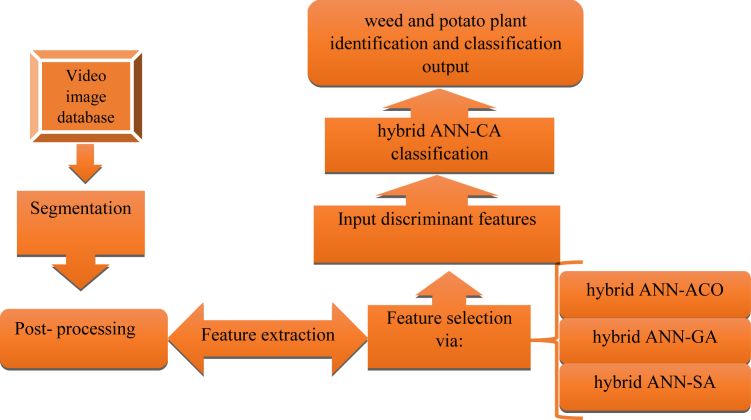
\includegraphics[width=0.5\linewidth]{./figures/workflow-sabzi.png}
	\caption[Color correction target and image set identification]{Example weed/crop classification workflow, adapted from \cite{Sabzi2020-af}. Raw images are segmented to isolate plants, from which various features are extracted. A feature selection step (using hybrid ANN with metaheuristic optimizers) selects important features, which are then fed into a classifier (here an ANN-Cultural Algorithm hybrid) to output weed vs. crop identification.}
	\label{fig:workflow-sabzi}
\end{figure}

% ([An automatic visible-range video weed detection, segmentation and classification prototype in potato field - PubMed](https://pubmed.ncbi.nlm.nih.gov/32490222/)) *Figure 1: Example weed/crop classification workflow, adapted from Sabzi et al. (2020). Raw images are segmented to isolate plants, from which various features are extracted. A feature selection step (using hybrid ANN with metaheuristic optimizers) selects important features, which are then fed into a classifier (here an ANN-Cultural Algorithm hybrid) to output weed vs. crop identification ([An automatic visible-range video weed detection, segmentation and classification prototype in potato field - PubMed](https://pubmed.ncbi.nlm.nih.gov/32490222/#:~:text=six%20hectares%20are%20used,Classification%20results)) ([An automatic visible-range video weed detection, segmentation and classification prototype in potato field - PubMed](https://pubmed.ncbi.nlm.nih.gov/32490222/#:~:text=being%20able%20to%20properly%20identify,15%20m%2Fs)).*  
%
\section{Addressing Class Imbalance}  
Class imbalance is a pervasive challenge to most classification problem and in weed/crop datasets. Often one class (usually the crop or a dominant weed) greatly outnumbers others. This imbalance can bias classifiers to favor the majority class, leading to poor detection of the minority class (e.g. a rare weed). Recent research \parencite{Wang2021-dh} has placed emphasis on \textit{balancing techniques} to ensure models learn both classes effectively:  

\begin{itemize}
	\item{Data Augmentation \& Synthesis: A straightforward approach is to generate more samples of the minority class. Hasan et al. (2021) constructed a large combined weed/crop image dataset from several smaller sets, then applied extensive image augmentations (rotations, flips, etc.) to mitigate class imbalance \parencite{Mahmudul-Hasan2023-ap}. This improved deep CNN recognition of under-represented weed species. Synthetic data generation techniques like GANs have also been explored to create new weed images, though with mixed success due to realism issues. } 

	\item{Oversampling Minority Class: Oversampling duplicates or creates new minority samples until the class distribution is more balanced. TheSynthetic Minority Oversampling Technique (SMOTE) is widely used  in agricultural datasets. SMOTE generates new synthetic examples along the line segments joining nearest-neighbor minority samples, effectively filling in gaps in feature space. For instance, Ahsen et al. (2024) applied SMOTE to balance weed and crop classes before training SVM and ANN classifiers, which led to improved accuracy on minority weed classes \parencite{Ahsen2024-dm}. An illustration of SMOTE’s effect is shown in Figure 2a – new minority points (green) are introduced between existing ones, alleviating the initial imbalance. However, SMOTE can also introduce overlap between classes if not careful (Figure 2b), as synthetic weeds may encroach on crop feature space. To combat this, variants likeSMOTE-ENN (which adds synthetic samples then applies Edited Nearest Neighbors to remove ambiguous points) have been employed. Bazrafkan et al. (2024) used a stratified sampling with SMOTE-ENN to balance a corn vs. weed polygon dataset, yielding a model with balanced precision and recall (\parencite{Bazrafkan2024-bl}). This reduced bias toward the majority (corn) and improved detection of minority weed instances.  }

	\item{Undersampling Majority Class: The opposite strategy is to downsample the majority class, training on a subset to match the minority count. While simple, this can discard useful data. In weed/crop studies, undersampling is less common than oversampling, since weed datasets are often limited \parencite{Mahmudul-Hasan2022-cj}. However, in cases where background or non-plant images vastly outnumber weed examples, controlled undersampling of background patches can help rebalance the training set.}  

	\item{Cost-Sensitive Learning: Instead of altering the data, algorithms can be made cost-sensitive, penalizing misclassification of minority classes more heavily. In weed detection, a higher misclassification cost can be assigned to weeds (the class of interest) so that the classifier prioritizes weed identification. Some recent deep learning models implicitly address imbalance by using focal loss or class-weighted loss functions to focus learning on hard-to-detect weeds \parencite{Wu2021-gt}. } 
\end{itemize}

Effect on Performance: Addressing class imbalance has proven crucial for reliable weed detection. Ramirez et al. (2021) showed that balancing the training data significantly improved weed segmentation accuracy in aerial images \parencite{Wu2021-gt}. In general, balanced datasets or effective oversampling yield models that detect both weed and crop classes more symmetrically (higher recall on weeds, and still high precision) \parencite{Bazrafkan2024-bl}. Table 2 highlights techniques used to handle class imbalance in recent studies. As seen, SMOTE and its variants are popular in machine learning approaches, while data augmentation is prevalent in deep learning approaches. Both strategies ultimately aim to provide the classifier with sufficient examples of weeds, which are often the minority class, thereby improving the generalization to those classes in test scenarios.  

{
% This avoids the document line spacing affecting the contents of the table
\setstretch{1.0}
% Example to span two pages
\begin{longtable}{x{\dimexpr.20\columnwidth-2\tabcolsep}
                  x{\dimexpr.20\columnwidth-2\tabcolsep}
                  x{\dimexpr.20\columnwidth-2\tabcolsep}
                  x{\dimexpr.20\columnwidth-2\tabcolsep}}
%\begin{hyphenrules}{nohyphenation}
    \caption{Techniques for Class Imbalance in Weed/Crop Classification}\label{tab:example}  \\
\toprule
{\textbf{Study}} & {\textbf{Issue}} & {\textbf{Technique}}  & {\textbf{Outcome}} 
\tabularnewline
\midrule
    \endfirsthead
%%%%
    \caption[]{Techniques for Class Imbalance in Weed/Crop Classification}\label{tab:example}  \\
\toprule
{\textbf{Study}} & {\textbf{Issue}} & {\textbf{Technique}}  & {\textbf{Outcome}} 
\tabularnewline
\midrule
    \endhead
%%%%
\midrule[\heavyrulewidth]
\multicolumn{4}{r}{\footnotesize\itshape
                   Continued on the next page}
    \endfoot
%%%%
\bottomrule
    \endlastfoot
Hasan et al. (2021) &
Combined weed datasets (multiple weed species, each with few samples) &
Data augmentation (flips, rotations) on minority classes; merge datasets &
Mitigated imbalance and improved deep CNN recognition of rare weed species. 
\tabularnewline\addlinespace
Ahsen et al. (2024) &
Early Crop-Weed (fewer weed images than crop) &
SMOTE oversampling for minority class before SVM/\gls{ANN} training &
Balanced class distribution led SVM to 99.5\% accuracy on minority-rich set (early crop-weed) and ANN to 89\% on CottonWeedID15, outperforming unbalanced training.
\tabularnewline\addlinespace
Bazrafkan et al. (2024) &
Corn vs weed polygons (weeds fewer than corn instances) &
SMOTE-ENN (SMOTE + cleaning) in Random Forest training  &
Achieved balanced precision/recall (~76\% accuracy). Improved weed recall by removing overlap and bias toward corn.
\tabularnewline\addlinespace
Dadashzadeh et al. (2020)  &
Rice vs weeds (two weed types vs crop, in field images) &
Metaheuristic feature selection + equalized training batches &
Selected features that best separate classes and used balanced batches for ANN training, yielding high accuracy (~95\%+) on both weed types. 
\tabularnewline\addlinespace
*Deep learning (various)* &
Weed classes underrepresented in images &
Class-weighted loss (e.g. focal loss) &
Enhanced detection of small weed clusters in dense crop fields (seen in segmentation CNNs), though not always explicitly reported in literature.  
\tabularnewline\addlinespace 
\label{table:class-imbalance}
\end{longtable}
}
%**Table 2. Techniques for Class Imbalance in Weed/Crop Classification**  
%
%| Study / Dataset         | Imbalance Issue                             | Technique Used                   | Outcome / Impact                               |
%|-------------------------|---------------------------------------------|----------------------------------|------------------------------------------------|
%| Hasan et al. (2021) ([[2112.07819] Weed Recognition using Deep Learning Techniques on Class-imbalanced Imagery](https://arxiv.org/abs/2112.07819#:~:text=MobileNetV2%2C%20and%20evaluated%20their%20performance,investigated%20the%20use%20of%20transfer))  | Combined weed datasets (multiple weed species, each with few samples) | Data augmentation (flips, rotations) on minority classes; merge datasets | Mitigated imbalance and improved deep CNN recognition of rare weed species. |
%| Ahsen et al. (2024) ([Precision Agriculture: Integrating Sensors for Weed Detection using Machine Learning in Agriculture Fields | Request PDF](https://www.researchgate.net/publication/388511045_Precision_Agriculture_Integrating_Sensors_for_Weed_Detection_using_Machine_Learning_in_Agriculture_Fields#:~:text=Learning%20,SMOTE%29%20to%20balance)) ([Precision Agriculture: Integrating Sensors for Weed Detection using Machine Learning in Agriculture Fields | Request PDF](https://www.researchgate.net/publication/388511045_Precision_Agriculture_Integrating_Sensors_for_Weed_Detection_using_Machine_Learning_in_Agriculture_Fields#:~:text=the%20classes,accuracy%20achieved%20underscores%20the%20practical)) | CottonWeedID15, Early Crop-Weed (fewer weed images than crop) | SMOTE oversampling for minority class before SVM/ANN training | Balanced class distribution led SVM to 99.5% accuracy on minority-rich set (early crop-weed) and ANN to 89% on CottonWeedID15, outperforming unbalanced training. |
%| Bazrafkan et al. (2024) ([A machine learning extension built on ArcGIS for the detection of weeds in cornfields](https://elibrary.asabe.org/azdez.asp?JID=5&AID=54934&Abstract=2400564.htm&CID=ana2024&T=3#:~:text=processing%2C%20including%20radiometric%20calibration%20during,approach%20was%20employed%20for%20model)) ([A machine learning extension built on ArcGIS for the detection of weeds in cornfields](https://elibrary.asabe.org/azdez.asp?JID=5&AID=54934&Abstract=2400564.htm&CID=ana2024&T=3#:~:text=data%20were%20then%20fed%20into,The%20model)) | Corn vs weed polygons (weeds fewer than corn instances) | SMOTE-ENN (SMOTE + cleaning) in Random Forest training | Achieved balanced precision/recall (~76% accuracy). Improved weed recall by removing overlap and bias toward corn. |
%| Dadashzadeh et al. (2020) ([Weed Classification for Site-Specific Weed Management Using an ...](https://www.mdpi.com/2223-7747/9/5/559#:~:text=,Plants%202020%2C%209%2C%20559)) ([Four typical plant datasets: (a) Grass-Broadleaf database [19], with... | Download Scientific Diagram](https://www.researchgate.net/figure/Four-typical-plant-datasets-a-Grass-Broadleaf-database-19-with-images-of-soybean_fig1_351846232#:~:text=,)) | Rice vs weeds (two weed types vs crop, in field images) | Metaheuristic feature selection + equalized training batches | Selected features that best separate classes and used balanced batches for ANN training, yielding high accuracy (~95%+) on both weed types. |
%| *Deep learning (various)* | Weed classes underrepresented in images    | Class-weighted loss (e.g. focal loss) | Enhanced detection of small weed clusters in dense crop fields (seen in segmentation CNNs), though not always explicitly reported in literature. |
%
% ([image]()) *Figure 2: Illustration of oversampling to address class imbalance (conceptual). (a) Initial imbalanced feature distribution: crop samples (orange) far outnumber weed samples (blue). (b) After applying SMOTE, synthetic weed samples (green points) are added, reducing imbalance. However, if placed unwisely, some synthetic points overlap with crop regions (overlap circled), which can degrade classifier performance ([Illustration of data synthesis by SMOTE: The initial imbalance... | Download Scientific Diagram](https://www.researchgate.net/figure/llustration-of-data-synthesis-by-SMOTE-The-initial-imbalance-condition-a-and-the_fig1_375505887#:~:text=,Therefore%2C%20SMOTE%20can%20potentially)). Techniques like SMOTE-ENN remove overlapping samples to mitigate this issue.*  
%
By applying these techniques, recent weed/crop classification models have become more resilient to skewed data, ensuring that even less common weeds can be reliably identified. Properly handling class imbalance is thus a key step toward practical field deployment of weed detection systems, where the prevalence of weeds can vary widely from plot to plot. In this work we will explore and test
techniques to dealing with class imbalance in order to improve the accuracy of the classifier algorithms.

\section{Image Segmentation Techniques}  
Segmentation isolates plant pixels from soil background (and sometimes separates crop vs. weed regions) so that features can be extracted reliably. Researchers have explored various segmentation methods, particularly focusing on the choice of color space to improve plant segmentation under real-world conditions.
%
\subsection{Segmentation with RGB based Color Indices}  
Many early methods operate directly in the RGB color space by exploiting the green color of vegetation. A common technique is \textit{color thresholding or color index segmentation}. For example, the excess green index ($ExG = 2G - R - B$) highlights green vegetation and can be thresholded to create a binary mask of plants vs. background \parencite{Wu2021-gt}. \citeauthor{Tang2000-an} proposed a modified color component approach using $ExG$ to segment weeds from soil, which proved effective in homogeneous lighting \parencite{Tang2000-an}. Similarly, simple thresholding on the green channel or ratios like $G/R$ can segment green plants in RGB images. These methods are fast and worked well in controlled conditions; Figure \ref{fig:segmentation-example} shows an example segmented mask where broadleaf and grass weeds were isolated from soil using such color difference techniques. However, RGB-based segmentation has limitations. The R, G, B channels are highly correlated and all vary with lighting intensity \parencite{Wu2021-gt}. Additionally, young crops and weeds can share similar RGB values, causing mis-segmentation when relying purely on greenness.

\begin{figure}[h!]
	\centering
	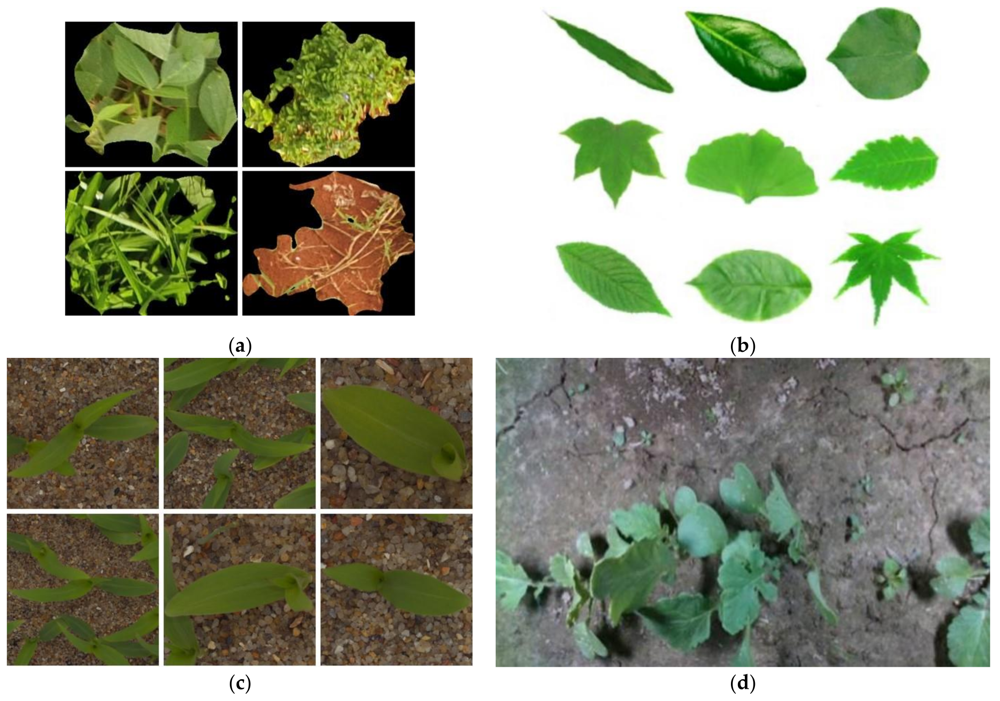
\includegraphics[width=0.5\linewidth]{./figures/segmentation-review.png}
	\caption[Examples of plant segmentation outcomes under different conditions]{Examples of plant segmentation outcomes under different conditions \parencite{Wu2021-gt}. Subfigure (a) Soybean crop (top-left) and weeds (broadleaf, grass) segmented from a complex background using color-index methods – black backgrounds here indicate extracted plant regions. Subfigure (b) Isolated leaf samples on uniform background (Flavia dataset) where simple thresholding suffices. Subfigure (c) Young maize seedlings in soil – segmentation challenges include varying soil color and lighting. Subfigure (d) Weeds amid crops in natural soil background – requiring advanced segmentation (e.g., machine learning or spectral methods) to separate weed plants from crop seedlings.}
	\label{fig:segmentation-example}
\end{figure}
%
% ([Review of Weed Detection Methods Based on Computer Vision](https://www.mdpi.com/1424-8220/21/11/3647)) *Figure 3: Examples of plant segmentation outcomes under different conditions (from Wu *et al.* ([Four typical plant datasets: (a) Grass-Broadleaf database [19], with... | Download Scientific Diagram](https://www.researchgate.net/figure/Four-typical-plant-datasets-a-Grass-Broadleaf-database-19-with-images-of-soybean_fig1_351846232#:~:text=,))).(a)** Soybean crop (top-left) and weeds (broadleaf, grass) segmented from a complex background using color-index methods – black backgrounds here indicate extracted plant regions.(b)** Isolated leaf samples on uniform background (Flavia dataset) where simple thresholding suffices.(c)** Young maize seedlings in soil – segmentation challenges include varying soil color and lighting.(d)** Weeds amid crops in natural soil background – requiring advanced segmentation (e.g., machine learning or spectral methods) to separate weed plants from crop seedlings.* ([Four typical plant datasets: (a) Grass-Broadleaf database [19], with... | Download Scientific Diagram](https://www.researchgate.net/figure/Four-typical-plant-datasets-a-Grass-Broadleaf-database-19-with-images-of-soybean_fig1_351846232#:~:text=,)) ([Four typical plant datasets: (a) Grass-Broadleaf database [19], with... | Download Scientific Diagram](https://www.researchgate.net/figure/Four-typical-plant-datasets-a-Grass-Broadleaf-database-19-with-images-of-soybean_fig1_351846232#:~:text=,))
%
To address RGB shortcomings, studies have introduced pre-processing steps to normalize lighting (e.g. illumination correction or applying contrast enhancement to make green plants more distinct) (\cite{Lu2022-rq}). Some recent work also uses machine learning to perform segmentation, such as training a classifier on pixel color features (RGB or indices) to label each pixel as plant or background (\cite{Gee2020-cz}). While effective, these still fundamentally rely on color cues. Thus, the choice of color representation is crucial, leading to exploration of alternative color spaces.
%
\subsection{Alternative Color Spaces  for Improved Segmentation}  
Converting images from RGB to a different color space can greatly improve segmentation robustness. Hue-Saturation-Value (HSV) and Hue-Saturation-Intensity (HSI) spaces separate color information (hue) from intensity, which helps under variable lighting. Hamuda et al. (2016) noted HSV aligns better with human color perception and is more robust to illumination changes \parencite{Hamuda2017-nf}. In practice, segmenting on the Hue channel (which represents “pure” color independent of brightness) can distinguish green plants from brown soil more reliably than raw RGB. \citeauthor{Priya2019-zw} found that extracting weed features in HSV yielded higher accuracy compared to using RGB \parencite{Priya2019-zw}. They converted field images to HSV and applied thresholds on Hue and Saturation to isolate weeds, achieving up to 95\% segmentation accuracy in their experiments . Figure 4 (top row) conceptually illustrates how an HSV-based segmentation might separate a weed (bright green hue) from soil (neutral hue) even when brightness varies – something harder to do in RGB. 
%
Other color spaces have also been tested: YCrCb/YIQ and related luminance-chrominance models isolate intensity (Y) from color components. Tang et al. (2017) used the YCbCr space to better capture green features of crops/weeds under different illumination, since the chrominance components Cb and Cr carry color detail unaffected by brightness \parencite{Wu2021-gt}. \citeauthor{Sabzi2020-af} identified the standard deviation of the \textit{in-phase} component (I) in the YIQ color space as one of six key features for weed discrimination \parencite{Sabzi2020-af} – implying that analyzing weeds in YIQ space highlighted differences not obvious in RGB. Likewise, CIELab (L*a*b*) space (with separate lightness channel L*) and Normalized Excess Green (nExG) are reported to improve segmentation by reducing sensitivity to shadows (\parencite{Wu2021-gt}). \citeauthor{Guo2013-eq} comprehensively evaluated 18 color features across six color spaces (RGB, YCbCr, HSL, HSV, CIELab, CIELuv), finding that combinations of channels (like a*, b* in Lab or Hue in HSV) can boost segmentation reliability (\cite{Guo2013-eq}).  
%
In summary, transforming to alternative color spaces allows threshold-based segmentation to leverage more stable color properties: hue for true color, chroma for color content, etc. These methods tend to outperform pure RGB segmentation especially under field conditions especially in the presence of shadows, dry/wet soil patches, or sun glare. Table \ref{tab:color-space} compares segmentation approaches using different color representations. As shown, HSV/HSI is frequently favored for its robustness, while YIQ/YCrCb and Lab are useful in specific scenarios. It’s worth noting that while color space conversion aids greatly, extremely complex scenes (e.g. overlapping crop and weed canopies) may still require advanced methods like deep learning segmentation (e.g. U-Net or Mask R-CNN) \parencite{Wu2021-gt}. Indeed, recent papers integrate both approaches – using color-index segmentation as a preprocessing step, then refining with machine learning or CNNs for pixel-level classification. Still, for many precision agriculture applications with relatively distinct crop and weed color, the combination of proper color space and simple thresholding provides an efficient solution on resource-limited farm equipment.
%
{
% This avoids the document line spacing affecting the contents of the table
\setstretch{1.0}
% Example to span two pages
\begin{longtable}{x{\dimexpr.20\columnwidth-2\tabcolsep}
                  x{\dimexpr.20\columnwidth-2\tabcolsep}
                  x{\dimexpr.20\columnwidth-2\tabcolsep}
                  x{\dimexpr.20\columnwidth-2\tabcolsep}
                  x{\dimexpr.20\columnwidth-2\tabcolsep}}
%\begin{hyphenrules}{nohyphenation}
    \caption{Color Space Segmentation Techniques in Weed/Crop Imaging}\label{tab:example}  \\
\toprule
{\textbf{Segmentation}} & {\textbf{Space}} & {\textbf{Context}}  & {\textbf{Notes}} & {\textbf{Reference} } 
\tabularnewline
\midrule
    \endfirsthead
%%%%
    \caption[]{Color Space Segmentation Techniques in Weed/Crop Imaging}\label{tab:example}  \\
\toprule
{\textbf{Segmentation}} & {\textbf{Space}} & {\textbf{Context}}  & {\textbf{Notes}} & {\textbf{Reference} } 
\tabularnewline
\midrule
    \endhead
%%%%
\midrule[\heavyrulewidth]
\multicolumn{5}{r}{\footnotesize\itshape
                   Continued on the next page}
    \endfoot
%%%%
\bottomrule
    \endlastfoot
Basic thresholding on Green or ExG &
RGB (indices) &
Green crops/weeds vs soil (uniform lighting) &
Fast and works in simple scenes; fails under lighting changes or similar-colored weeds/crops. &
Tang et al. (2017) Hamuda et al. (2016)
\tabularnewline\addlinespace 
 HSV-based segmentation &
 HSV/HSI &
 Outdoor fields with variable illumination &
 Robust to lighting; separates color from intensity. Successfully used for weed detection in cauliflower and other crops &
 Hamuda et al. (2016) Jeba Priya et al. (2019)
 \tabularnewline\addlinespace 
 YCbCr or YIQ chrominance threshold &
 YCbCr, YIQ &
 Scenarios with shadows or faded colors &
 Using chrominance (Cb, Cr or I, Q) isolates color information unaffected by brightness. Tang et al. leveraged YCrCb for consistent green detection under varying light. Sabzi et al. used YIQ-I for feature extraction, implying segmentation utility &
 Tang et al. (2017) Sabzi et al. (2020)
  \tabularnewline\addlinespace 
Lab color space segmentation &
CIELab &
Variable soil backgrounds, multi-color plants &
Lab’s a* (green–red) and b* (blue–yellow) channels can be thresholded to pick out green vegetation. More robust to illumination than RGB, but not as intuitive as HSV. Used in some weed studies with success  &
Guo et al. (2018)
\tabularnewline\addlinespace 
Deep learning segmentation (CNNs)  &
*Any (learned)* &
Complex scenes (dense foliage, overlap) &
Learns color and texture cues automatically. Requires lots of data; can surpass static color threshold methods in difficult cases. E.g., Mask R-CNN on weeds improved segmentation of overlapping leaves &
Patidar et al. (2021) Yu et al. (2021)
\tabularnewline\addlinespace 

\label{tab:color-space}
\end{longtable}
}

%**Table 3. Comparison of Color Space Segmentation Techniques in Weed/Crop Imaging**  
%
%| Segmentation Method                 | Color Space    | Application Context                | Effectiveness and Notes                                    | Reference |
%|-------------------------------------|---------------|------------------------------------|------------------------------------------------------------|-----------|
%| Basic thresholding on Green or ExG  | RGB (indices)  | Green crops/weeds vs soil (uniform lighting) | Fast and works in simple scenes; fails under lighting changes or similar-colored weeds/crops. | Tang et al. (2017) ([Review of Weed Detection Methods Based on Computer Vision](https://www.mdpi.com/1424-8220/21/11/3647#:~:text=using%20the%20difference%20in%20color,harvest%20cereals%2C%20which)); Hamuda et al. (2016) ([Review of Weed Detection Methods Based on Computer Vision](https://www.mdpi.com/1424-8220/21/11/3647#:~:text=size%2C%20and%20position,89%5D%20used%20the%20color)) |
%| HSV-based segmentation              | HSV/HSI        | Outdoor fields with variable illumination | Robust to lighting; separates color from intensity. Successfully used for weed detection in cauliflower and other crops ([Review of Weed Detection Methods Based on Computer Vision](https://www.mdpi.com/1424-8220/21/11/3647#:~:text=spaces%2C%20such%20as%20HIS%2C%20HSV%2C,Knoll%20et%20al)). Jeba Priya et al. reported ~95% accuracy using HSV thresholds ([](https://www.ijrte.org/wp-content/uploads/papers/v8i1/A1191058119.pdf#:~:text=farm,accuracy%20comparing%20to%20other%20methods)). | Hamuda et al. (2016) ([Review of Weed Detection Methods Based on Computer Vision](https://www.mdpi.com/1424-8220/21/11/3647#:~:text=spaces%2C%20such%20as%20HIS%2C%20HSV%2C,Knoll%20et%20al)); Jeba Priya et al. (2019) ([](https://www.ijrte.org/wp-content/uploads/papers/v8i1/A1191058119.pdf#:~:text=farm,accuracy%20comparing%20to%20other%20methods)) |
%| YCbCr or YIQ chrominance threshold  | YCbCr, YIQ     | Scenarios with shadows or faded colors | Using chrominance (Cb, Cr or I, Q) isolates color information unaffected by brightness. Tang et al. leveraged YCrCb for consistent green detection under varying light ([Review of Weed Detection Methods Based on Computer Vision](https://www.mdpi.com/1424-8220/21/11/3647#:~:text=Therefore%2C%20many%20methods%20transform%20images,Knoll%20et%20al)). Sabzi et al. used YIQ-I for feature extraction, implying segmentation utility ([An automatic visible-range video weed detection, segmentation and classification prototype in potato field - PubMed](https://pubmed.ncbi.nlm.nih.gov/32490222/#:~:text=six%20hectares%20are%20used,Classification%20results)). | Tang et al. (2017) ([Review of Weed Detection Methods Based on Computer Vision](https://www.mdpi.com/1424-8220/21/11/3647#:~:text=Therefore%2C%20many%20methods%20transform%20images,Knoll%20et%20al)); Sabzi et al. (2020) ([An automatic visible-range video weed detection, segmentation and classification prototype in potato field - PubMed](https://pubmed.ncbi.nlm.nih.gov/32490222/#:~:text=six%20hectares%20are%20used,Classification%20results)) |
%| Lab color space segmentation        | CIELab         | Variable soil backgrounds, multi-color plants | Lab’s a* (green–red) and b* (blue–yellow) channels can be thresholded to pick out green vegetation. More robust to illumination than RGB, but not as intuitive as HSV. Used in some weed studies with success ([Review of Weed Detection Methods Based on Computer Vision](https://www.mdpi.com/1424-8220/21/11/3647#:~:text=spaces%2C%20such%20as%20HIS%2C%20HSV%2C,Knoll%20et%20al)) ([Review of Weed Detection Methods Based on Computer Vision](https://www.mdpi.com/1424-8220/21/11/3647#:~:text=illumination%20conditions,also%20utilized%20different%20color%20spaces)). | Guo et al. (2018) ([Review of Weed Detection Methods Based on Computer Vision](https://www.mdpi.com/1424-8220/21/11/3647#:~:text=illumination%20conditions,also%20utilized%20different%20color%20spaces)) |
%| Deep learning segmentation (CNNs)   | *Any (learned)*| Complex scenes (dense foliage, overlap) | Learns color and texture cues automatically. Requires lots of data; can surpass static color threshold methods in difficult cases. E.g., Mask R-CNN on weeds improved segmentation of overlapping leaves ([Review of Weed Detection Methods Based on Computer Vision](https://www.mdpi.com/1424-8220/21/11/3647#:~:text=semantic%20information%20made%20the%20experimental,methods%20do%20not%20rely%20on)). Often preceded by converting images to an effective color space for input. | Patidar et al. (2021) ([Review of Weed Detection Methods Based on Computer Vision](https://www.mdpi.com/1424-8220/21/11/3647#:~:text=semantic%20information%20made%20the%20experimental,methods%20do%20not%20rely%20on)); Yu et al. (2021) ([Review of Weed Detection Methods Based on Computer Vision](https://www.mdpi.com/1424-8220/21/11/3647#:~:text=CNNs%20are%20increasingly%20used%20in,The%20experimental%20results%20showed)) |
%
In practice, a combination of methods may be more robust. For example, apply an HSV threshold to quickly segment vegetation, then use morphological filters or a classifier to refine the mask. The overall trend  is to move away from pure RGB segmentation towards approaches that exploit more perceptually uniform color spaces (HSV, Lab) and even incorporate learning for segmentation. This has substantially improved the quality of weed segmentation masks, which in turn boosts the accuracy of subsequent classification of those segments as weed or crop  \parencite{Wu2021-gt}.
%
\section{Final Thoughts} 
Over the last few years, weed/crop classification research has evolved from purely hand-crafted feature approaches to more integrated methods addressing data and environmental challenges. Texture, shape, and color features remain highly relevant – studies consistently show that combining these features yields superior results than any single feature alone, as each captures different aspects of plant variance  The advent of deep learning has not obviated the need for such features; rather, it has shifted some focus to automatically learning them, but many practical systems still rely on engineered features due to limited data or the need for interpretable models in agriculture.  
%
A critical realization in recent work is the importance of class balance in model training. Techniques like SMOTE and targeted data augmentation have become common when preparing weed datasets, ensuring that rare weed classes (often the ones of greatest interest for herbicide targeting) are learned adequately \parencite{Ahsen2024-tr, Bazrafkan2024-bl}. Without these, even the best feature sets can lead to biased classifiers that miss the minority class. The literature illustrates various success stories in balancing strategies – from simple oversampling to sophisticated GAN-based oversamplers – all reinforcing the idea that a classifier is only as good as the data it sees. Figure  \ref{fig:segmentation-example}’s depiction of SMOTE pitfalls showed that oversampling must be done carefully; domain-specific oversampling (e.g. only within weed clusters in feature space, or using weed images from slightly different fields) can avoid generating implausible samples.  
%
In the scope of image segmentation, the use of alternate color spaces (HSV, HSI, YCrCb, YIQ, Lab) has clearly improved the extraction of plant regions from images  \parencite{Wu2021-gt}. Segmenting weeds from crops is the first step of many pipelines, and mistakes at this stage (e.g. losing part of a weed leaf to the background) directly reduce classification accuracy. By choosing color representations that are invariant to common field lighting issues, researchers have achieved more stable segmentation. This is evident in comparative studies where HSV-based methods outperformed RGB by a significant margin \parencite{Priya2019-zw}. At the same time, the field is gradually embracing machine learning for segmentation (e.g. semantic segmentation CNNs that label each pixel as crop/weed/soil), which can handle extremely challenging scenes. A few recent works combined traditional color thresholding with deep segmentation to get the best of both approaches – quick initial segmentation and detailed refinement.  
%
Weed/crop classification research since 2018 demonstrates a robust toolbox of techniques: from GLCM textures to Hu moments to excess-green thresholds and HSV conversions. Table \ref{table:previous-studies} and Table \ref{tab:color-space} provided in this review encapsulate key findings and methods. Development of more hybrid approaches are anticipated: for example, using deep networks that explicitly incorporate texture or shape priors, or adaptive sampling techniques that address class imbalance on the fly. The challenge of real-world deployment (on robots or tractors) also means computational efficiency is crucial – something hand-crafted features and clever color space tricks are well-suited for, compared to heavyweight deep models. By building on the advances in feature extraction, data balancing, and segmentation, future systems are poised to achieve reliable, real-time weed detection to enable site-specific weed management and reduce herbicide usage. Prior work points to  a strong foundation for these machine vision assisted intelligent, sustainable, and cost effective farming solutions to the weeds challenge.
%
%

Problems commonly encountered in weed/crop classification systems include items that are addressed by this study, including:

\begin{itemize}

\item{Young weeds and crop seedlings often look very similar in terms of color, shape, and texture, especially during early growth stages, complicating accurate identification. This work will show that the two classes can be distinguished more accurately when considering features that have not been more thoroughly explored (such as texture in non-RGB color spaces}

\item{Both weeds and crops undergo significant changes in appearance as they grow, meaning classification models need to adapt dynamically across different growth stages. This work will explore the impact of these changes over the early stages, and test these factors for seasonal changes.}

\item{Datasets often have many more crop samples than weed samples, leading to biased training and poor generalization on rare weed species. This work will investigate the impacts of correction on classification.}

\item{Complex algorithms, particularly deep learning models, require substantial computational resources, limiting real-time deployment on farm equipment. While this work will not discuss the topic of optimizing software for resource constrained deployment environments, it does consider the computational cost to achieve a result.}

\item{High-quality, annotated field data is often scarce or expensive to obtain, hindering the training and validation of robust models. While not a development or deployment issue, this is the primary motivation for the image collection associated with this work.}

\end{itemize}


% Original Introduction begin
%\section{Introduction and Prior Work}
%While precision treatment of unwanted vegetation, positive treatment of desired vegetation, or simply assessment of a crop may be the end goal, classifying vegetation in the acquired images is the first major step in that workflow. 
%This paper concentrates on the binary classification of vegetation into two discrete classes: desired vegetation (cantaloupe) and undesired vegetation (weeds and crop occupying an undesired position). Once classified, vegetation can be treated using a variety of mechanical, chemical~(\cite{Saile2022-vu}), or no-touch~(\cite{Saile2022-vu,Mwitta2022-yt}) methods. The specifics of and integration with the treatment system are beyond the scope of this document, but treatment considerations will be discussed within the context of establishing a buffer zone around desired vegetation to minimize crop damage.
%
%Irrespective of the treatment details, accuracy is key. According to the USDA, Arizona alone produced over \$411M in head lettuce in 2023 \parencite{USDA2023-wb}. Even seemingly minor  increases in the accurate identification of vegetation have profound economic impacts. Misclassification of crop followed by a negative treatment results in a lower yield; Misclassification of a weed followed by the absence of a negative treatment may result in competition between crop that can be sold and weeds that cannot. Even a 1\% change represents millions of dollars in affected crop.
%
%This study seeks to answer several questions:
%\begin{enumerate}
%	\item{Can shape, color, and texture attributes be used to predict vegetation class?}
%	\item{Is classification affected by developmental changes in vegetation across the development cycle?}
%	\item{Can imbalanced datasets be used in classification?}
%\end{enumerate}
%
%While it is tempting to use the terms \textit{weed} and \textit{crop} (and this document will often use those terms), this proposal will more often reference vegetation as \textit{desired} (crop in the position wanted) and \textit{undesired} (weeds and crop not in the position wanted).  That is, classification more often answers the question ``do we want this plant?'' than ``is this plant a weed?''. These two questions are often conflated, but are subtly distinct. As will be discussed in a later section, a plant may be desirable in one growing season, and undesired in another, complicating attempts at classification.
%
%Images from UAVs offer several advantages over those obtained with manned aircraft and satellite, such as the economics or flexibility of acquisition, but this study will leverage the relative ease with which UAVs are able to gather imagery from various distances close to the ground. These distances are much closer to the ground than are more typically encountered partially out of pragmatism. While the images are also gathered using ground-based cameras, image acquisition through low-level AUV flights is a convenient work-around for the author's physical limitations, as well as providing images directly after irrigation, when even access by walking through the planting beds is limited. Additionally, images gather via UAV typically have a more complete view of the vegetation, allowing shape features to be explored.
% 
%\citeauthor{Ong2023-lm}, in a study of classification of Chinese Cabbage, classifies vegetation acquired at an average of 2m AGL using a single set of attributes, Local Binary Pattern (LBP, a texture descriptor), and a single approach (Random Forest) leveraging those attributes, validating the use of texture in classification \parencite{Ong2023-lm}. \citeauthor{Etienne2021-ik}, in a study of Corn and Soybean plots, used imagery gathered from both 10m and 30m AGL. but found that the best training set for selected algorithm (YOLOv3) was taken from the set of images acquired from 10m \parencite{Etienne2021-ik}. The parameters selected as significant to classification fall into three basic categories: shape, color, and texture. Variants of each of these categories will be used in this study. 
%In a study of weed mapping in sunflower crop, \citeauthor{Perez-Ortiz2015-yk} present findings from images taken from three distances AGL, 30m, 60m, and 100m, classifying each pixel as crop, weed, or soil using SVM, KNN, and k-means (and variants of those) approaches \parencite{Perez-Ortiz2015-yk}. While this approach does indeed yield weed maps that lend themselves to later study, the approach is a bit different in terms of what is being classified. In that study, individual pixels are being classified, in contrast to this study that seeks to classify individual plants.
%In a study of weeds in corn, \citeauthor{Lin2017-xq} used shape metrics as part of the classification workflow, stressing the importance of expressing shape metrics that are not rotationally variant. More importantly, the study details a shape metric possessing the desired qualities for use in classification. Using shape and texture (GLCM), the study demonstrated an overall accuracy exceeding 95\%.\footnote{\citeauthor{Lin2017-xq}'s study did not report some items that are of interest: the distances of the imagery to the camera, and the false positive rate of weed identification. While the high overall rate sounds is certainly impressive, that metric will not be used in this study. Additionally, the images of vegetation were acquired under controlled conditions, something that is not reproducible in the field an at higher distances AGL.} \citeauthor{Sabzi2020-af}, in a study of a potato field, used various channels of color spaces (YIQ, YCbCr, HSI) as well as texture (Grey-Level Co-occurrence Matrix, GLCM) to achieve a high correct classification rate, but the use of GLCM is not applied  to channels of the color conversion, only to RGB images that have been converted to greyscale \parencite{Sabzi2020-af}. While this is a conventional use of the texture identification technique, it does not leverage the information content available in other color spaces.
%
%Shape and texture analysis is not limited to plants, of course, \citeauthor{Bankman2009-wq}, detailing shape and texture quantification in medical images, steps through many of the techniques employed here, particularly the concept of \textit{radial distance} \parencite{Bankman2009-wq}. While there is clear overlap between the techniques of medical image analysis and the analysis of agricultural images in areas such as textural analysis, the concepts and techniques around shape analysis are of particular interest.

% Original introduction end

%\section{Goals and Expectations}
%The goal of this study is to classify vegetation with high accuracy (exceeding 90\%) for classification using color, texture, or shape, with higher accuracy achieved using a combination of those attributes. 

\newpage
\chapter{Methodology}
\label{section:methodology}
This methodology section outlines the comprehensive approach adopted for weed and crop classification. The workflow comprises four key stages: image acquisition, segmentation, feature extraction, and classification. Initially, high-quality images are collected using various sensors under diverse environmental conditions to ensure a robust dataset. Following image acquisition, segmentation techniques are employed to delineate and isolate regions of interest, effectively separating crops from weeds and background noise. Next, a suite of discriminative features—ranging from color and texture to shape descriptors—is extracted to characterize the segmented regions. Finally, advanced classification algorithms are applied to these features to accurately differentiate between crop and weed classes. Each stage is discussed in detail in the subsequent sections, highlighting the challenges encountered and the strategies implemented to overcome them, ultimately contributing to the development of a reliable and efficient weed/crop classification system.

This study will seek to answer several questions:
\begin{itemize}
	\item{Can texture expressions in color spaces other than greyscale be used to categorize vegetation? That is, a traditional expression of texture is an expression of a portion of a greyscale image. Is the expression of texture in a channel of another color space (such as YIQ) usable?}
	\item{What can be achieved with various traditional classification techniques (SVM, KNN, Random Forest, etc.) using a specific type of attribute (shape, color, texture)?}
	\item{What is the optimal set of attributes for various traditional classification techniques. That is, if all types of attributes are considered, what is the best set for a technique?}
	\item{Do attributes change over the crop development cycle?}
	\item{What is the computational cost of achieving a given result?}
\end{itemize}

To answer these questions, a set of crop images will be collected, processed, and analyzed. The collection will be appropriate for the needs of a ground-based system: towed or self-propelled. These systems will acquire images at the distances considered (within 1m above ground level, AGL).


%\section{Data Preparation}
%Images discussed in this study comes in two forms: static images obtained with visible light cameras and prepared images of manually manipulated scenarios.  Manipulated images are used throughout this document to illustrate concepts and for testing purposes, but are not used in classification. Manipulations include tasks such as inserting weeds, manipulating color-balance, changing exposure, etc. Feature analysis and machine learning use unmanipulated images exclusively, while tests will be conducted on a mixture of the two. 

% Omit descriptions of prepared images 

%\subsection{Discrete Static Images}
%Discrete image sets are those acquired in the field with an RGB camera. The image sets used in this analysis was acquired using three sources: a Samsung SM-G930V phone, an iPhone 14 Pro, and a DJI Air 2s. These images often have vegetation at the edges of the image, and frequently of only a single plant, attempts to classify vegetation considering shape  can lead to poor results. As Figure~\ref{fig:problem-cropline} shows, a crop-line cannot be determined or surmised using only a single crop image. In this instance, the crop-line is assumed to be along the center-line of the image. Figure~\ref{fig:problem-cutoff} demonstrates the problem encountered where the shape of an object cannot be used as a factor in classification, as the shape is distorted by having a regular, straight edge.
%
%% Side by side subfigures 
%\begin{figure}[H]
%	\begin{subfigure}[h]{0.48\linewidth}
%		\includegraphics[width=1\linewidth]{./figures/problem-cropline.jpg}
%		\caption{The crop-line cannot be determined.}
%		\label{fig:problem-cropline}
%		
%	\end{subfigure}
%	\hfill
%	\begin{subfigure}[h]{0.48\linewidth}
%		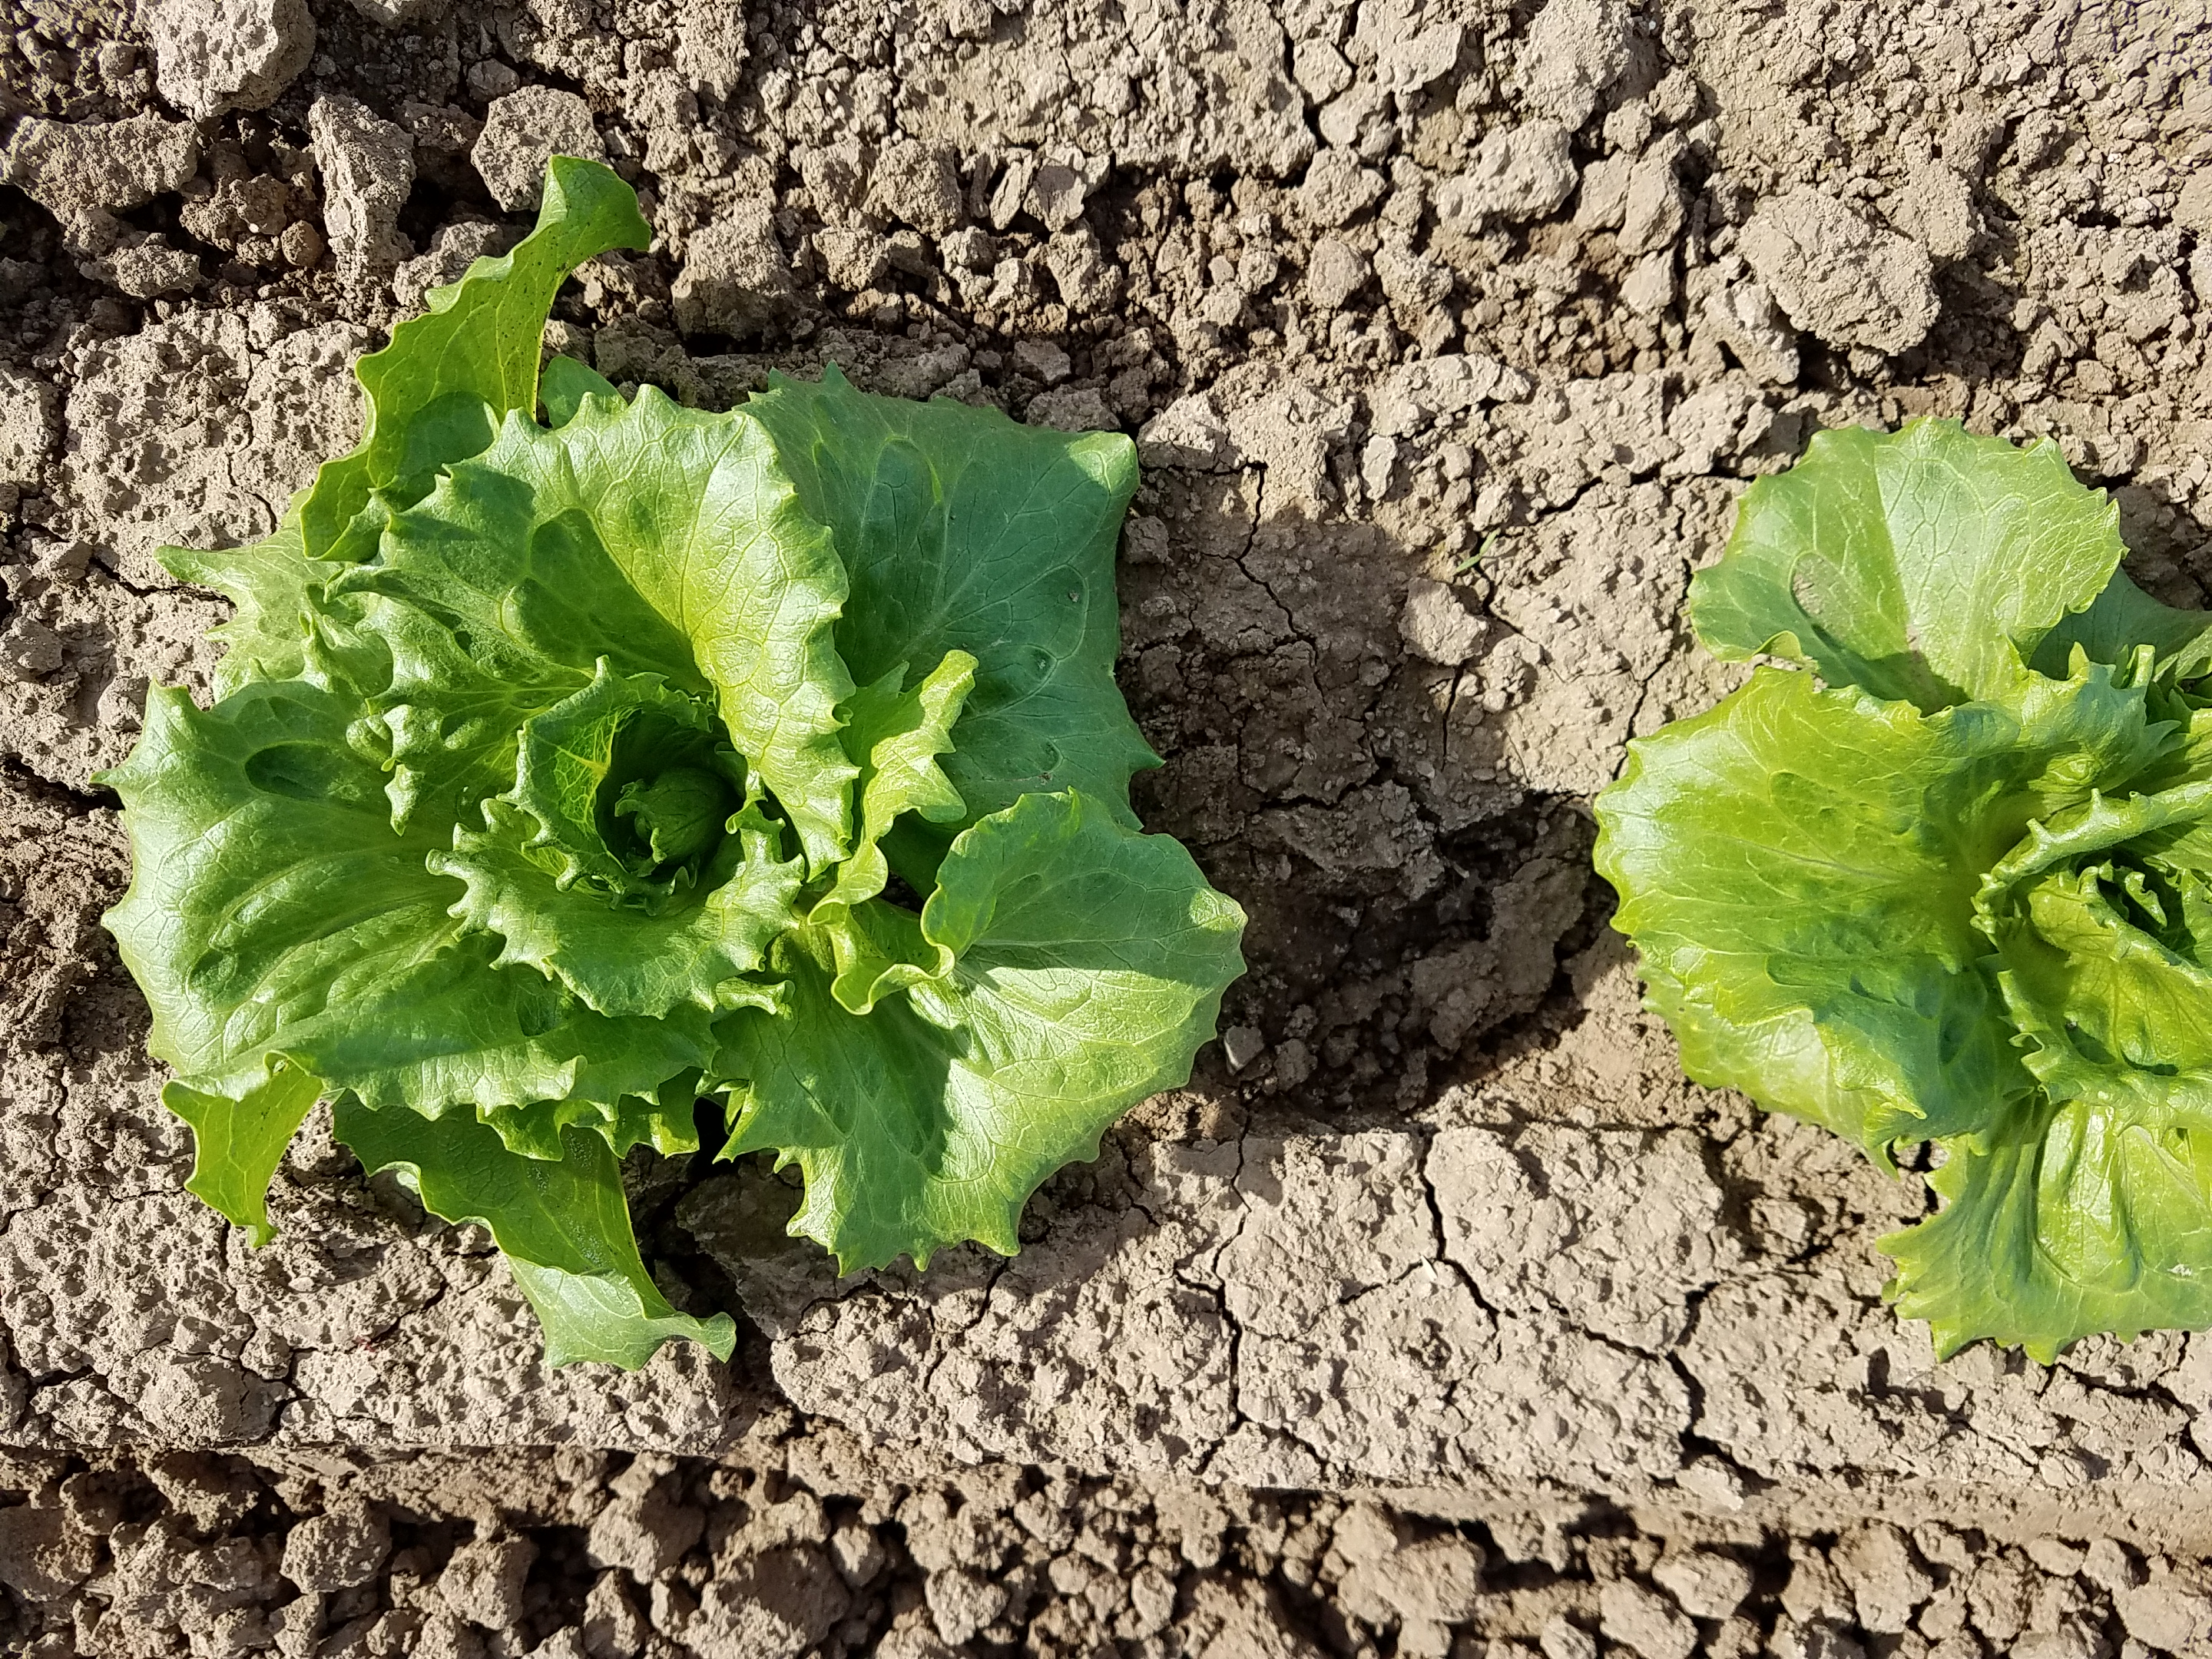
\includegraphics[width=1\linewidth]{./figures/problem-cutoff.jpg}
%		\caption{The vegetation is cut off.}
%		\label{fig:problem-cutoff}		
%	\end{subfigure}%
%	\caption[Common problems in field images]{These cases illustrate common problems encountered in image sets where the crop-line cannot be conclusively determined (\ref{fig:problem-cropline}) and the cutoff of vegetation (\ref{fig:problem-cutoff}). In the case where images contain a single image of crop the intended crop-line cannot be automatically determined. In the case where vegetation is cut off along the edges of the image shape analysis cannot be used, as otherwise the shape of the vegetation is distorted by the clean, straight edge. \textit{Source: Dr.~Mark Siemens, University of Arizona}}
%\end{figure}
%
%
%
%\subsection{Prepared Images}
%Test images acquired in the field are prepared using Adobe Photoshop\textsuperscript{\textregistered} to create test data for various scenarios:
%\begin{itemize}
%	\item{The presence of a specific weed in the image.}.
%	\item{Debris in the image -- this is the case where non-vegetated matter appears in the image. While the image segmentation discussed in section \ref{section:segmentation} should result in non-vegetated matter being removed, inserting both expected (irrigation equipment) and unexpected (human litter) into the images is a mechanism to test various scenarios.}
%\end{itemize}
%
%\begin{figure*}[h]
%	\begin{subfigure}[t]{0.48\linewidth}
%		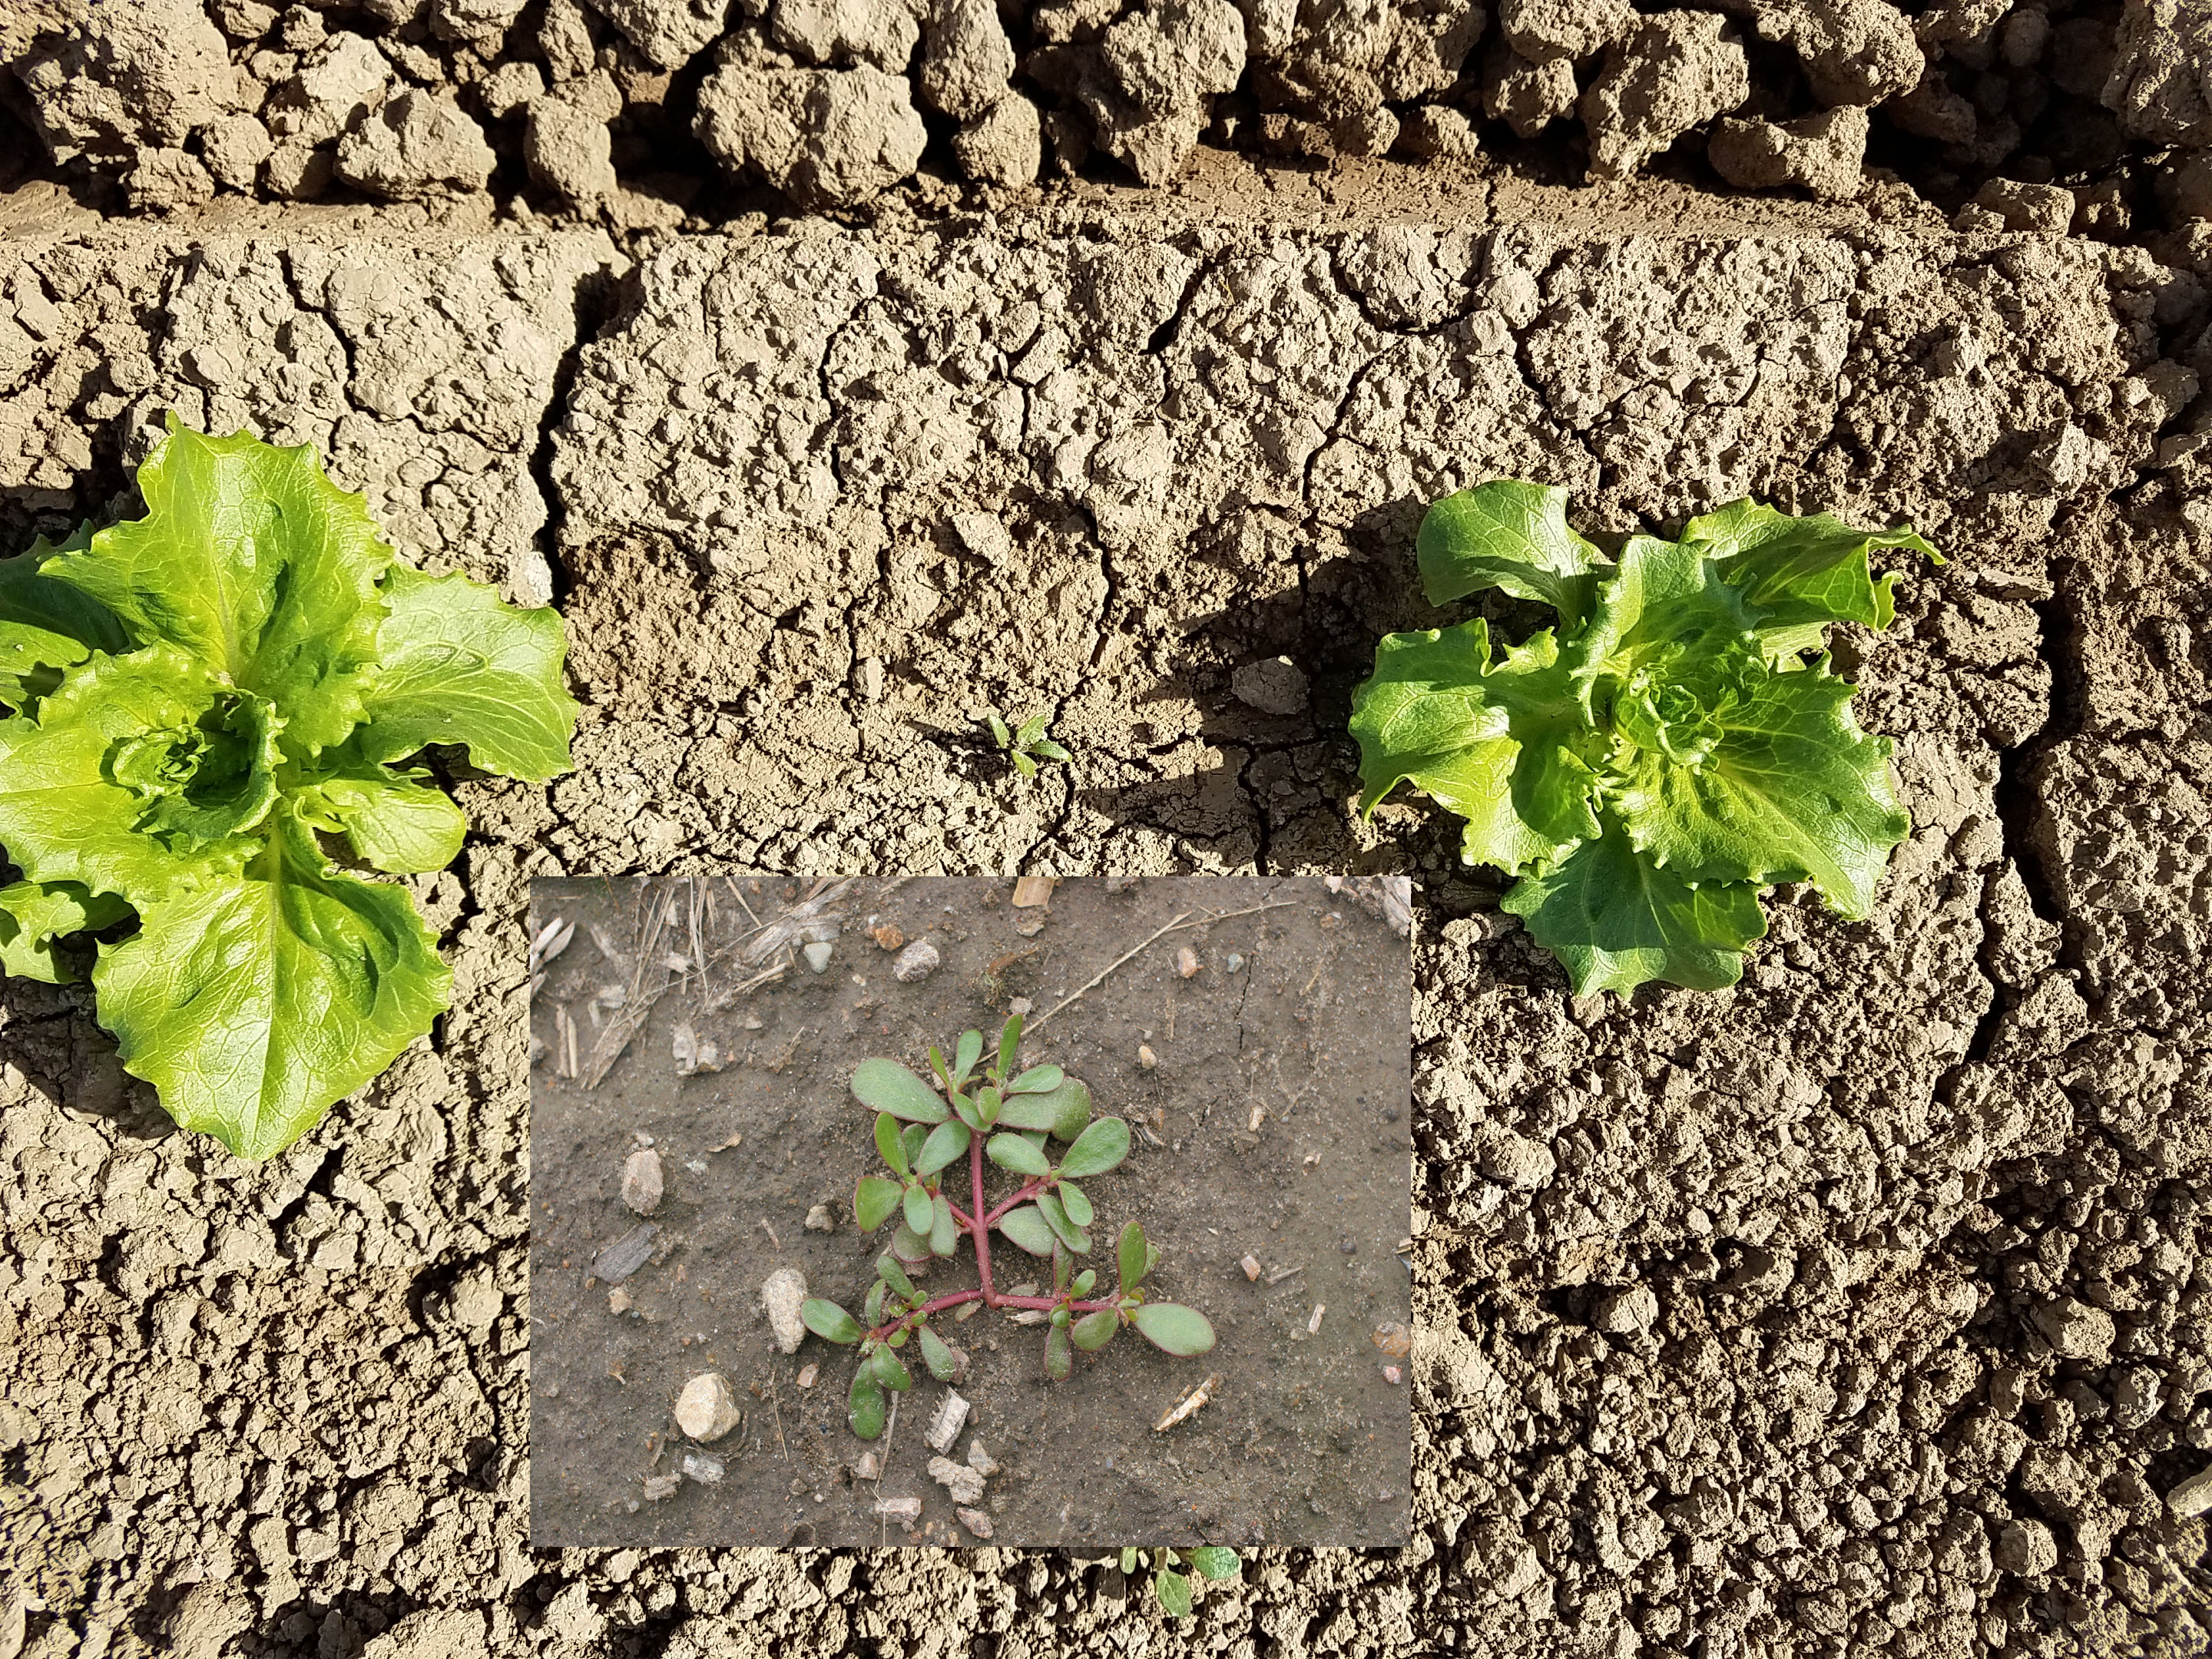
\includegraphics[width=1\linewidth]{./figures/with-purslane.jpg}
%		\caption{Purslane (\textit Portulaca oleracea) inserted.}
%		\label{fig:prepared-weed}
%	\end{subfigure}
%	\hfill
%	%
%	% TODO: Replace this image with one where irrigation equipment is inserted into image
%	%
%	\begin{subfigure}[t]{0.48\linewidth}
%		\includegraphics[width=1\linewidth]{./figures/cantaloupe-with-lid.jpg}
%		\caption{Identifying lid beside plant.}
%		\label{fig:prepared-lid}		
%	\end{subfigure}%
%	\caption[Prepared images]{Images acquired in the field are subsequently manipulated by either inserting images of weeds not already present (\ref{fig:prepared-weed}), or inserting non-vegetated items (\ref{fig:prepared-lid}). Both cases are intended to present situations that should be handled by the classification algorithms. \\ \textit{Manipulated images: (\ref{fig:prepared-weed}) Dr. Mark Siemens, University of Arizona}}
%\end{figure*}
%
%
%Here, vegetation is placed within separate layers to create a composite image that shows the desired result.  Figure~\ref{fig:prepared-weed} illustrates the basic technique that is used to form a single image of both crop and a weed. This figure shows several differences that are immediately obvious: scale differences, as the weed image was obtained at a different distance, and lighting difference, as the weed image was obtained at a different location. Inserting a weed into an image solely for the purposes of classification has little value, of course, as classification of separate images is equivalent. The intent of this is to test the effect of the weed's proximity to the crop. Images are also manipulated to test certain scenarios, as Figure \ref{fig:prepared-lid} shows. A bucket lid with dots used to identify a specific plant is inserted into the image to test two things: the exclusion of the bucket lid itself, and the identification of the lid and plant it is closest to.


\section{Classification Approach}
%The goal of this processing flow is to determine and classify the image contents as desired or undesired. Besides weeds, crop plants can also be classified as \textit{undesired} in they should be  thinned, as such this work will use the term \textit{undesired} and \textit{weed} interchangeably. Vegetation in an image falls into one of these classifications:
%\begin{itemize}
%	\item{Desired, the crop}
%	\item{Undesired, weeds that can be treated without crop damage}
%	\item{Unknown, vegetation that cannot be confidently identified}
%	\item{Ignored, vegetation that is too close to desired vegetation to be treated without crop damage}
%\end{itemize}
%
%Additionally, this work makes a few simplifying assumptions about the images:
%\begin{itemize}
%	\item{The crop typically follows straight and consistent lines, deviating by only a few degrees on average.}
%	\item{Weeds grow in a random pattern and can appear anywhere, so weed centers are typically not in horizontal alignment.}
%	\item{Crop is typically much larger than weeds.}
%\end{itemize}
To thoroughly evaluate the performance of various approaches for crop and weed classification, nine distinct classification methods were examined. The study includes ensemble-based algorithms such as Random Forest, Gradient Boosting, and Extra Trees, which are renowned for their ability to handle high-dimensional and noisy datasets. In addition, traditional classifiers like K-Nearest Neighbors (KNN), Logistic Regression, and Decision Tree offer insights into more interpretable and straightforward modeling techniques. Furthermore, Support Vector Machines (SVM) and Linear Discriminant Analysis (LDA) were employed to assess the efficacy of margin-based and linear projection methods, respectively, while a Multi-Layer Perceptron (\gls{MLP}) was integrated to explore the potential benefits of neural network architectures. This diverse methodological framework enables a comprehensive comparison, highlighting the strengths and limitations of each technique in distinguishing between crops and weeds.

%While the desired crop is usually homogenous in size, follows a precise line, and tend to be larger than weeds, there are exceptions. For instance, a weed may be in perfect alignment within a crop line and two other plants. Each of these observations, however, are used in classification. Take, for instance, the observation that crop tends to be much larger than weeds. If the size of an item is three times that of another, the smaller item is -- more likely than not -- a weed. Another exception comes from orientation. Commonly encountered in images acquired with an automated platform, but less so with manually acquired ground images is that vegetation does not appear in horizontal or vertical orientation, complicating simplistic attempts to classify off-horizontal or off-vertical vegetation as weeds.

%\begin{figure}[H]
%	\centering
%	\includegraphics[width=0.48\linewidth]{./figures/crop-alignment}
%	\caption[Crop may not be in perfect horizontal or vertical alignment in images acquired]{Crop may not be in perfect horizontal or vertical alignment in images acquired autonomously. In this drone image, the crop is not in an alignment that would lend itself to crop identification in either orientation, as the crop-lines are along diagonals through the image.}
%	\label{fig:alignment}	
%\end{figure}

%\section {Study Area}
%This study will be carried out at the University of Arizona Maricopa Agricultural Center (\gls{MAC}) on a cantaloupe crop (Spring 2024) and broccoli crop (Fall 2024) overseen by Drs. Attalah and Elshikha (University of Arizona), as part of another study.\footnote{The field in question is located at N 33.061805$^{\circ}$ W 111.966162$^{\circ}$} That study will involve three separate water treatments: center-pivot, flood irrigation, and drip. As the drip treatment study area is unlikely to produce a heavy weed load, it will not be included in this study, as differentiating between crop and weeds is an initial goal of this study. The study site is relatively free of obstacles that would impact low level flight with one notable exception: the center pivot irrigation system. Allowances will be made to avoid that system, but doing so is not expected to affect flight plans, as images in only subset of the field is planned to be captured.
 

\section{Software Tools Considerations}
Both commercial and open-source software were used in the development of this study. While the majority of the software (the operational portions responsible for image processing and classification) was written in Python, commercial packages were used for pre-processing. Additionally, R was used in visualization and analysis of classification results. The complete source code for this project is available in this GitHub repository: \href{https://github.com/evan-mcginnis/weeds}{\textit {weeds}}. Images, both raw and processed, are far too large to be hosted with GitHub, and are available on request from the author.

All development was done on Windows 10 PC (11th Gen Intel(R) Core(TM) i7-11700F @ 2.50GHz with 32GB RAM) and Ubuntu 18.04.06 with analysis on the University of Arizona's \textit{High Performance Compute Cluster}.

{
% This avoids the document line spacing affecting the contents of the table
\setstretch{1.0}
\begin{longtable}{x{\dimexpr.20\columnwidth-2\tabcolsep}
                  x{\dimexpr.20\columnwidth-2\tabcolsep}
                  x{\dimexpr.5\columnwidth-2\tabcolsep}}
%\begin{hyphenrules}{nohyphenation}
    \caption{Software Used}\label{tab:software}  \\
\toprule
{\textbf{Component}} & {\textbf{Use}} & {\textbf{Comment}}
\tabularnewline
\midrule
    \endfirsthead
%%%%
    \caption[]{Software Used (cont.)}\label{tab:software}  \\
\toprule
{\textbf{Component}} & {\textbf{Use}} & {\textbf{Comment}}
\tabularnewline
\midrule
    \endhead
%%%%
\midrule[\heavyrulewidth]
\multicolumn{3}{r}{\footnotesize\itshape
                   Continued on the next page}
    \endfoot
%%%%
\bottomrule
    \endlastfoot
%%%%
		PyCharm 
		& Python IDE     
		& Commercial software for Python development
\tabularnewline\addlinespace
		Python 3.9     
		& Python runtime                    
		& Most software was written in python
\tabularnewline\addlinespace
		scikit-learn
		& Machine Learning     
		& Implementations for various ML techniques 
\tabularnewline\addlinespace
		imbalance-learn
		& Class Imbalance     
		& Various imbalance correction techniques  
\tabularnewline\addlinespace
		OpenCV2 
		& Image Processing     
		& Machine Vision and Image Processing framework
\tabularnewline\addlinespace
		Numpy
		& Numeric Processing   
		& Python library
\tabularnewline\addlinespace
		Pandas 
		& Numeric Processing     
		& Python library
\tabularnewline\addlinespace
		PyQT5 
		& UI     
		& User Interface Framework for Python
\tabularnewline\addlinespace
		R 
		& Post Processing     
		& Statistical Software
\tabularnewline\addlinespace
		Plotly
		& Visualization     
		& Graphing libraries
\tabularnewline\addlinespace
		Adobe Lightroom
		& Color Correction     
		& Commercial software used for pre-processing
\tabularnewline\addlinespace
		Adobe Photoshop
		& Image preparation     
		& Commercial software used for image manipulation
\tabularnewline\addlinespace
		Dronelink
		& UAV Control     
		& Commercial software used for planning \& control
\tabularnewline\addlinespace
		MongoDB
		& Image organization     
		& No-SQL database 
\tabularnewline\addlinespace
		Docker Container
		& Virtualization     
		& Virtual containers host database and web server
\tabularnewline\addlinespace
		Slurm
		& Workload     
		& Supercomputer workload management
\label{table:software}
\end{longtable}
}

Minor use was made of C++ (a compiled language) and PyCuda, a library allowing access to a GPU when exploring performance improvements, but  that use was not key to the findings presented here.

\section{Processing Pipeline}
Images are processed following the pipeline shown in Figure~\ref{fig:workflow}. Each step in this workflow will be discussed in subsequent sections. The example images and analysis within the next few sections are taken from a set of images supplied by Dr. Mark Siemens, University of Arizona, and as such are not expected to provide an exact match to those acquired under the field conditions of this study. These images, however, are useful in the demonstration of key techniques. This image set of 39 images was taken in 2019 with a Samsung SM-G930V phone. The pipeline illustrated supports the notion of supervised learning, where a human classifies plants that are then used in a model for predicting the plant's class. That is, the two pipelines are identical, with the sole difference being that a model replaces the human in classification. 
\begin{figure}[H]
	\centering
	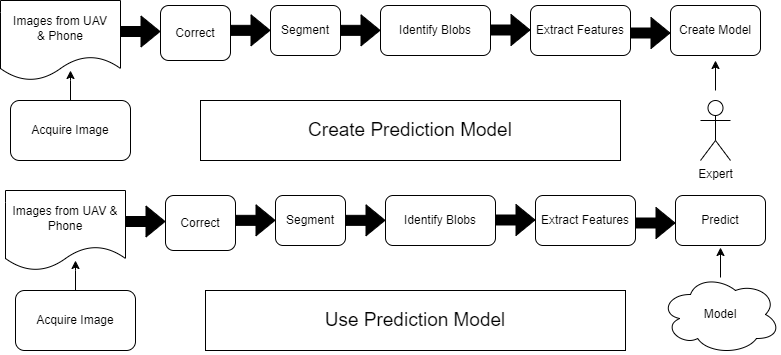
\includegraphics[width=0.85\linewidth]{./figures/workflow.png}
	\caption[Image processing workflow]{Image processing piplines. There are two pipelines followed, the creation of the model (where a human classifies the vegetation in the image) and use of that model to predict the plant.}
	\label{fig:workflow}	
\end{figure}


\section{Acquire Image}
Image acquisitions were carried out at the University of Arizona Maricopa Agricultural Center (\gls{MAC}) on a cantaloupe planting (N $33.061857^\circ$, E $111.967145^\circ$) consisting of 3 water treatments: flood, drip, and center-pivot, each watered at 80\% and 100\%. The field location coordinates were acquired using an Apple iPhone 14 Pro using the \textit{GPSCoordinates} application from the Apple Store. The field was used for an unrelated study of irrigation impacts, but was otherwise typical of what could be expected of a field used for commercial production.
Only the flood and pivot treatments will be imaged and considered for this study. This is mostly motivated by practical considerations: it is not anticipated that the drip treatment plots will have a significant number of weeds.  Image acquisition occurred at regular intervals beginning in April 2024 and continuing through May 2024 (Cantaloupe), and October 2024 continuing through November 2024 (Broccoli).  Ambient lighting conditions during acquisitions were quite similar, as they were carried out around the same time (mid-morning) and under (almost) cloudless skies.

Images were captured at two elevations (\gls{AGL}): 20cm \& 1m, approximating the camera position of a ground-based system (towed or self-propelled). While it is unrealistic to acquire images at such low altitudes for an entire field, the development of a machine learning model requires only a small subset of the field, and these images allow ground truth to be established just by image inspection. 

With the exception of images taken from 20cm, all images were acquired using a DJI Mavic Air 2S with a stock RGB 20 MP camera with the following specifications:

\begin{itemize}
	\item{13.25mm sensor width}
	\item{8.38mm focal length}
	\item{5464 pixel width}
	\item{3640 pixel height}
\end{itemize}

Images gathered at 20cm were taken with an iPhone 14 Pro, using the 48MP main camera.

\begin{itemize}
	\item{7.3mm sensor width}
	\item{8.38mm focal length}
	\item{8063 pixel width}
	\item{6048 pixel height}
\end{itemize}

The drone flight altitude is unrealistically low, but this is mostly because the UAV was treated more as a flying camera that allowed images to be acquired shortly after irrigation, and avoided requiring entering the field even when conditions allowed. The class of a plant could be manually confirmed at 2 meters, but those from higher altitudes could not be. Other pragmatic concerns must also be considered. UAVs can acquire images in situations where ground acquisition (towed, self-propelled, or even a phone camera on a stick) are infeasible due to field conditions (a field might realistically inaccessible for several days after irrigation or precipitation event).


Each image acquisition activity was accompanied by an image of a \href{https://www.datacolor.com/spyder/products/spyder-checkr-photo/} {SpyderChecker 24} color calibration chart (under the same ambient lighting conditions) and color correction was subsequently applied using Adobe Photoshop Lightroom Classic and custom calibration profiles created using the Spyder Checkr software. Raw sensor data from both camera systems was stored in Adobe Digital Negative (DNG) format before color correction and conversion to a JPG format for the resulting images. The digital negative of each image (DNG, a standard format for raw sensor data) was corrected and converted to JPG format for subsequent processing. The merits of raw, uncompressed, and unprocessed sensor data versus compressed, processed formats like JPG are beyond the scope of this document, but it is fair to say taking raw sensor data, processing, and then producing a compressed JPG is precisely what consumer products like phone cameras do. So that the color correction step can be inserted, the process of producing an image that can be viewed with most software is altered a bit, but essentially unchanged from what would be expected from a consumer device. The images in all digital cameras start out as the values from a sensor; many cameras simply provide this in a convenient to use format, and JPG is the most widely usable. It is also fair to say that a format like JPG does not actually represent what the sensor ``sees'', but is the result of the in-camera processing of sensor data. This workflow also results in a JPG image set, but separates image acquisition from processing. Color correction, for instance, is more than a bit easier with raw sensor data than a JPG due to  the much wider color spectrum present in the raw sensor data (16.7 million vs 68.7 billion is a big difference). The camera sensor data for each image was quite large, requiring 38.5 MB of storage, with equivalent JPG images much smaller.
Where feasible, missions were conducted in the same ambient light conditions, but an exact match of ambient conditions using uncontrolled lighting is not always possible. As all missions took place in mid-morning under cloudless skies, the resulting image sets are fairly closely matched in terms of illumination and color temperature.

\begin{figure}[h!]
	\centering
	\includegraphics[width=0.8\linewidth]{./figures/color-correction.jpg}
	\caption[Color correction target and image set identification]{All images are color corrected for each set. Prior to each collection, this photo was taken with the camera used for the acquisition. The color target captured was subsequently used to create a correction profile for that image set using software supplied by the vendor.}
	\label{fig:color-correction}
\end{figure}

\subsection{UAV Mission Planning}
Missions for UAV flights were planned and executed with Dronelink software, a commercially available package.  Where feasible, missions were conducted in the same ambient light conditions, but an exact match of ambient conditions using uncontrolled lighting is not always possible.
As illustrated by Figure \ref{fig:field-layout} the largest flood irrigated area is \SI{4536}{\metre\squared}, a location where image acquisition took place.  

%Consider the size of the ground captured with a UAV flight at various heights:
%
%\begin{table*}[h!] \centering
%\begin{tabular}{SSSSSSSS} \toprule
%    {AGL (m)} & {Captured Width (m)} & {Images} \\ \midrule
%    1  & 2 & xxx \\
%    2  & 3  & xxx  \\
%    5  & 8  & xxx  \\
%    10  &16  & xxx     \\ \bottomrule
%\end{tabular}
%\caption{Ground captured at various distances AGL}
%\label{table:captured}
%\end{table*}
% Metadata altitude analysis is with this command
% python altitude.py -i d:\maricopa\corrected\2024-05-08\flood-1m d:\maricopa\corrected\2024-05-08\pivot-2m d:\maricopa\corrected\2024-05-08\pivot-5m d:\maricopa\corrected\2024-05-08\flood-10m
The capture area spans the width of three plots at 10 meters AGL. While the missions are planned for these heights, environmental factors (wind) and positional accuracy may result in variance of the actual distance AGL achieved and consequently the effective image resolution. While both factors will vary from one mission to another, the image metadata examined from a mission executed on 8 May 2024 shows fairly low standard deviation values for the elevation  at various heights: 0.06m (1m AGL), 0.08m (2m AGL), 0.08m (5m AGL), and 0.05m (10m AGL). Positional accuracy, as it relates to ground location was not assessed in this study. While an RTK solution could certainly improve positional accuracy along all axes in reporting the exact location of an image, such precision is not particularly relevant to this study, as absolute location will not be used as a factor in classification.

\begin{figure}[h!]
	\centering
	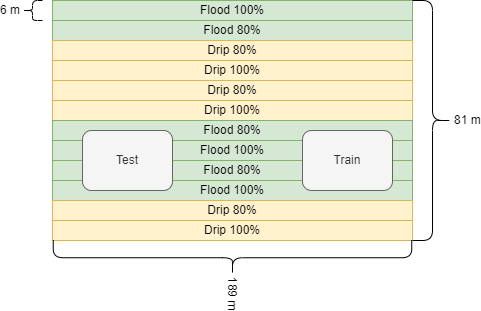
\includegraphics[width=0.8\linewidth]{./figures/test-area.png}
	\caption[Field layout for image acquisition]{The train and test subsets of the 80\% and 100\% water treatment of  flood irrigation is considered for this study. As the drip irrigation is not likely to show many weeds, it was not considered for this study.}
	\label{fig:field-layout}
\end{figure}

%Images were color, white-balance, and exposure corrected against images taken before each flight of a Spyder CHECKR24 calibration target using Adobe Lightroom$^{\circledR}$. The digital negative of each image (DNG, a standard format for raw sensor data) was corrected and converted to JPG format for subsequent processing.\footnote{The merits of raw, uncompressed, and unprocessed sensor data versus compressed, processed formats like JPG are beyond the scope of this document, but it is fair to say taking raw sensor data, processing, and then producing a compressed JPG is precisely what consumer products like phone cameras do. So that the color correction step can be inserted, the process of producing an image that can be viewed with most software is altered a bit, but essentially unchanged from what would be expected from a consumer device. The images in all digital cameras start out as the values from a sensor; many cameras simply provide this in a convenient to use format, and JPG is the most widely usable. It is also fair to say that a format like JPG does not actually represent what the sensor ``sees'', but is the result of the in-camera processing of sensor data. This workflow also results in a JPG image set, but separates image acquisition from processing. Color correction, for instance, is more than a bit easier with raw sensor data than a JPG due to  the much wider color spectrum present in the raw sensor data (16.7 million vs 68.7 billion is a big difference)}



As illustrated in Figure \ref{fig:field-layout}, the train and test image sets acquired were physically separate. The goal being that objects in the training subset should never appear in the testing subset. The side-lap and front-lap of UAV acquired images makes this task much more difficult, although any set of images of adjacent objects will exhibit this complication. Consider a UAV image acquisition of three plants, as shown in Figure \ref{fig:uav-overlap}. In this example, plants (even if it is only a portion) appear in multiple images. While this is expected -- and even desired for stitching the images together -- this complicates splitting the image set into train and test segments such that the same plant does not appear in both segments. The most practical approach here is to simply avoid the problem by not performing a split at all. An alternative approach was considered and rejected: stitching together all images to form one large one, and then dividing the image up. This approach would not solve the problem of a plant appearing in both segments. Collecting, instead, a completely separate train and test set of images. This approach has an additional benefit in that a test set can now be acquired from a different part of the field. Consider the case where the test set is taken from the \textit{drip} treatment area. While it will not have a particularly high weed load, it should be possible to classify the crop in that image set with the same accuracy as seen in the image set taken in the \textit{flood} treatment. While this study did not examine classification accuracy across water treatment methods, the clean separation of the train and test segments also means that test segments can be captured for different crops or different portions of the same field.

\begin{figure}[h!]
	\centering
	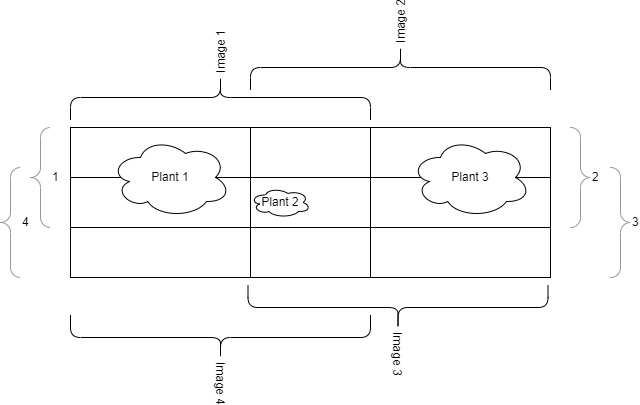
\includegraphics[width=0.5\linewidth]{./figures/overlap.png}
	\caption[Image overlap in UAV images]{The same plant appears in multiple images. As seen here, plants \#1 and \#3 appear in two (fully in images \#1 and \#2, partially in images \#3 and \#4), and plant \#3 appears in full in four images. A train/test split is possible, of course, but requires knowledge of what an image contains.}
	\label{fig:uav-overlap}
\end{figure}

%
% B U C K E T  L I D S
%
% This does not add value
%
%To identify specific plants from various altitudes, distinct objects were placed on the ground near the plants to be sampled. For this purpose, round bucket lids with a unique set of dots applied to identify each lid were used. The plant nearest the center of the lid could then be identified from various altitudes as well as in various image sets. While the results of verifying the features of the same plant from various altitudes is not presented in further detail here, confirming that details used were invariant with altitude was part of this study.
%
%
%\begin{figure}[h!]
%	\centering
%	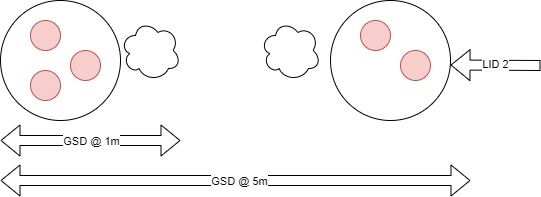
\includegraphics[width=8cm]{./figures/lids.jpg}
%	\label{fig:bucket-lids}
%	\caption[Identification of specific plants using bucket lids]{Bucket lids with a unique number of round stickers applied to them are used to identify specific plants from various altitudes. At lower distances AGL only a single plant may be in view. At higher distances AGL, however, multiple plants and multiple lids might be in view or the plant may be shifted within the frame. This necessitates having a mechanism to uniquely identify a specific lid. The number of stickers uniquely identifies the lid and stickers are identified in the image by their shape. The intent of this is not so much to identify the lid as it is to identify the closest vegetation to that lid.}
%\end{figure}	
%
%Bucket lids are identified by the number of colored stickers they contain -- fortunately the stickers are an easily identifiable, uniform shape: a circle. Identifying a lid consists of two steps: isolating the lids from everything else in the image, and identifying the stickers. For lid isolation, the image is segmented just as would be done with isolating vegetation. In this case, the image is converted to the HSV space and only those pixels with the blue hue of the bucket lid appear in the final image. Round shapes are identified in the segmented image using a variant of the Hough Transform \parencite{Ballard1981-oc}. The most salient limitation to this technique, of course is that a round object that has the same hue of blue as the lid will be identified as a lid. This limitation may be a hindrance to using this technique more widely on a diverse set of images, but will suffice for the purpose of this study.
%
%% Use of subfloat aligns the bottom of images -- important when figures are of different heights
%\begin{figure}[H]
%	\centering
%	\subfloat[Segmented bucket lid]{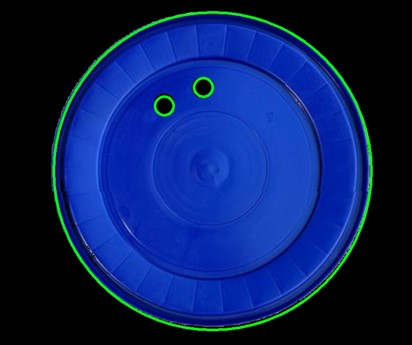
\includegraphics[width=6cm]{./figures/lid-segmented.jpg}\label{fig:bucket-segmented}}
%	\hfil
%	\subfloat[Lid beside crop]{\includegraphics[width=8cm]{./figures/DJI_0321.jpg}\label{fig:bucket-lid-with-plants}}
%	\caption[Identification of specific bucket lids]{The lids themselves are isolated the same way vegetation is, by applying an index. In this case, the index isolates the blue hue found in the lid, but is not found in the study area. The stickers on the lid and the lid itself are both an easily detected shape, a circle. This figure shows both treatments: the lid itself is separated from the background and circles within the image are highlighted in green. This image shows bucket lid \# 2, as three circles are found: one for the lid itself, and two stickers. Identification of the circle that is the lid is more important than it first appears, as only those stickers completely contained within the lid contribute to its identity. Figure \ref{bucket-lid-with-plants} illustrates the challenge of identifying the same plant across images -- here we see multiple plants, and it is not immediately clear which plant is closest to the center of the lid.}
%\end{figure}	
%
% I M A G E  S E G M E N T A T I O N
%
\section{Segment Image}
\label{section:segmentation}
To pre-process the image before further analysis is done, image segmentation must be done.  Image segmentation is a fundamental step in image processing, particularly in applications where separating objects from their background is essential for analysis. In agricultural and environmental studies, segmenting vegetation from soil or distinguishing between plant species is a critical task. The least compute-intensive portion of this workflow is to discard the portion of an image that does not contribute meaningfully to classification. For this problem notably, non vegetated pixels representing the ground. There are three segmentation approaches considered for this task: index-based, threshold based, and deep-learning based. The result of each of these approaches is the same: the portions of the images that did not contain pixels with vegetation present were discarded by creating a mask using one of the techniques and applying that mask to the original image to both isolate the vegetation and reduce the information content. This discards both the ground and debris while retaining any active desired and undesired vegetation. 

\subsection{RGB Index Based}
Index-based segmentation relies on mathematical transformations of pixel values to enhance the distinction between different classes in an image. These transformations, commonly referred to as vegetation indices, are designed to highlight features of interest, such as chlorophyll content in plants, by leveraging differences in spectral reflectance across color channels. By applying a threshold to these indices, an effective binary segmentation mask can be created, distinguishing target objects (e.g., plants) from their background (e.g., soil or non-vegetation areas). Index-based segmentation methods are widely used due to their simplicity, speed, and ability to process large datasets efficiently. Unlike machine learning-based segmentation, which requires labeled training data and computationally expensive model training, index-based approaches operate on predefined mathematical formulas. These methods are particularly beneficial in real-time applications, such as automated weed detection in precision agriculture, where rapid processing is essential.
For this study, images were segmented using various visible light indices (\cite{Hunt2013-ih}, \cite{Hamuda2016-dw}).  Various approaches to image segmentation are  summarized in Table \ref{table:segmentation}.  

{\renewcommand{\arraystretch}{2}%

{
% This avoids the document line spacing affecting the contents of the table
\setstretch{1.0}
% Example to span two pages
\begin{longtable}{x{\dimexpr.25\columnwidth-2\tabcolsep}
                  x{\dimexpr.35\columnwidth-2\tabcolsep}
                  x{\dimexpr.4\columnwidth-2\tabcolsep}}
%\begin{hyphenrules}{nohyphenation}
    \caption{Visible light indices}\label{tab:example}  \\
\toprule
{\textbf{Index}} & {\textbf{Formula}} & {\textbf{Comment}}
\tabularnewline
\midrule
    \endfirsthead
%%%%
    \caption[]{Visible light indices}\label{tab:example}  \\
\toprule
{\textbf{Index}} & {\textbf{Formula}} & {\textbf{Comment}}
\tabularnewline
\midrule
    \endhead
%%%%
\midrule[\heavyrulewidth]
\multicolumn{3}{r}{\footnotesize\itshape
                   Continued on the next page}
    \endfoot
%%%%
\bottomrule
    \endlastfoot
%%%%
		Triangular Greenness
		& \begin{minipage}[t]{0.3\textwidth}
			$R_{green} - \alpha R_{red} - \beta R_{blue}\\ \alpha = \frac {2(\lambda_{blue} - \lambda_{green})} {(\lambda_{blue} - \lambda_{red})}\\ 
		    	\beta = \frac {2(\lambda_{green} - \lambda_{red})} {(\lambda_{blue} - \lambda_{red})} $
		   \end{minipage}     
		& Corrects for camera calibration using the peak sensitivity
\tabularnewline\addlinespace

		Normalized Difference     
		& $128 * \left( \left( \frac {(G - R)} {(G + R)} \right) + 1 \right) $                    
		& The NDI index produces a near-binary image. 
\tabularnewline\addlinespace

		Excess Green      
		& \begin{minipage}[t]{0.3\textwidth}
			$R = \frac {R} {R_{max}}\\ G = \frac {G} {G_{max}}\\ B = \frac {B} {B_{max}}$ 
		   \end{minipage}
		& ExG provided a clear contrast between plants and soil 
\tabularnewline\addlinespace

		Excess Red      
		& $1.3 R - G$ 
		& inspired by the fact that there are 4\% blue, and 32\% green, compared with 64\% red cones in the retina of the human eye
\tabularnewline\addlinespace

		Color Index of Vegetation Extraction      
		& $0.441 R - 0.811 G + 0.385 B + 18.78745$
		& This method was proposed to separate green plants from soil background in order to evaluate the crop growing status.
\tabularnewline\addlinespace

		Excess Green - Excess Red   
		& $ExG - ExR$ 
		& ExG used to extract the plant region and ExR used to eliminate the background noise (soil and residue) where green–red material (stems, branches, or petioles) may exist
\tabularnewline\addlinespace

		Normalized Green-Red Difference    
		& $\frac {(G - R)} {(G + R)}$ 
		& The method of NGRDI was used to overcome the differences in exposure settings selected by the digital camera when acquiring aerial photography of the field. 
\tabularnewline\addlinespace

		Vegetative Index      
		& $\frac {G} {R^aB^{(1-a)}}, a = 0.667$ 
		& VEG has a significant advantage because it is robust to lighting change.
\tabularnewline\addlinespace

		Com1   
		& $ExG + CIVE + ExGR + VEG$ 
		& High computational cost --- does not perform well in high or low light levels
\tabularnewline\addlinespace

		Modified Excess Green      
		& $1.262G - 0.884R = 0.311B$ 
		& Does not perform well in high or low light levels. 
\tabularnewline\addlinespace

		Combined Indices 2      
		& $0.36ExG + 0.47CIVE + 0.17VEG$ 
		& Uses weighting factors to emphasize strengths of various approaches
%\tabularnewline\addlinespace
\label{table:indices}
\end{longtable}
}

These indices are used to create a mask that is then applied to the original source image to permit vegetation to show while masking details that are not relevant (ground pixels, stones, and other items that may appear in field conditions such as irrigation equipment) The intent here is to remove all pixels that are not relevant to the task of distinguishing between crop and weed while leaving the vegetated pixels unmanipulated.

\begin{figure}[H]
	\centering
	\begin{subfigure}[h]{.30\textwidth}
	  \centering
	  \includegraphics[width=1\linewidth]{figures/original.jpg}
	  \caption{Field view of lettuce and weed}
	  \label{fig:original}
	\end{subfigure}
	\begin{subfigure}[h]{.30\textwidth}
	  \centering
	  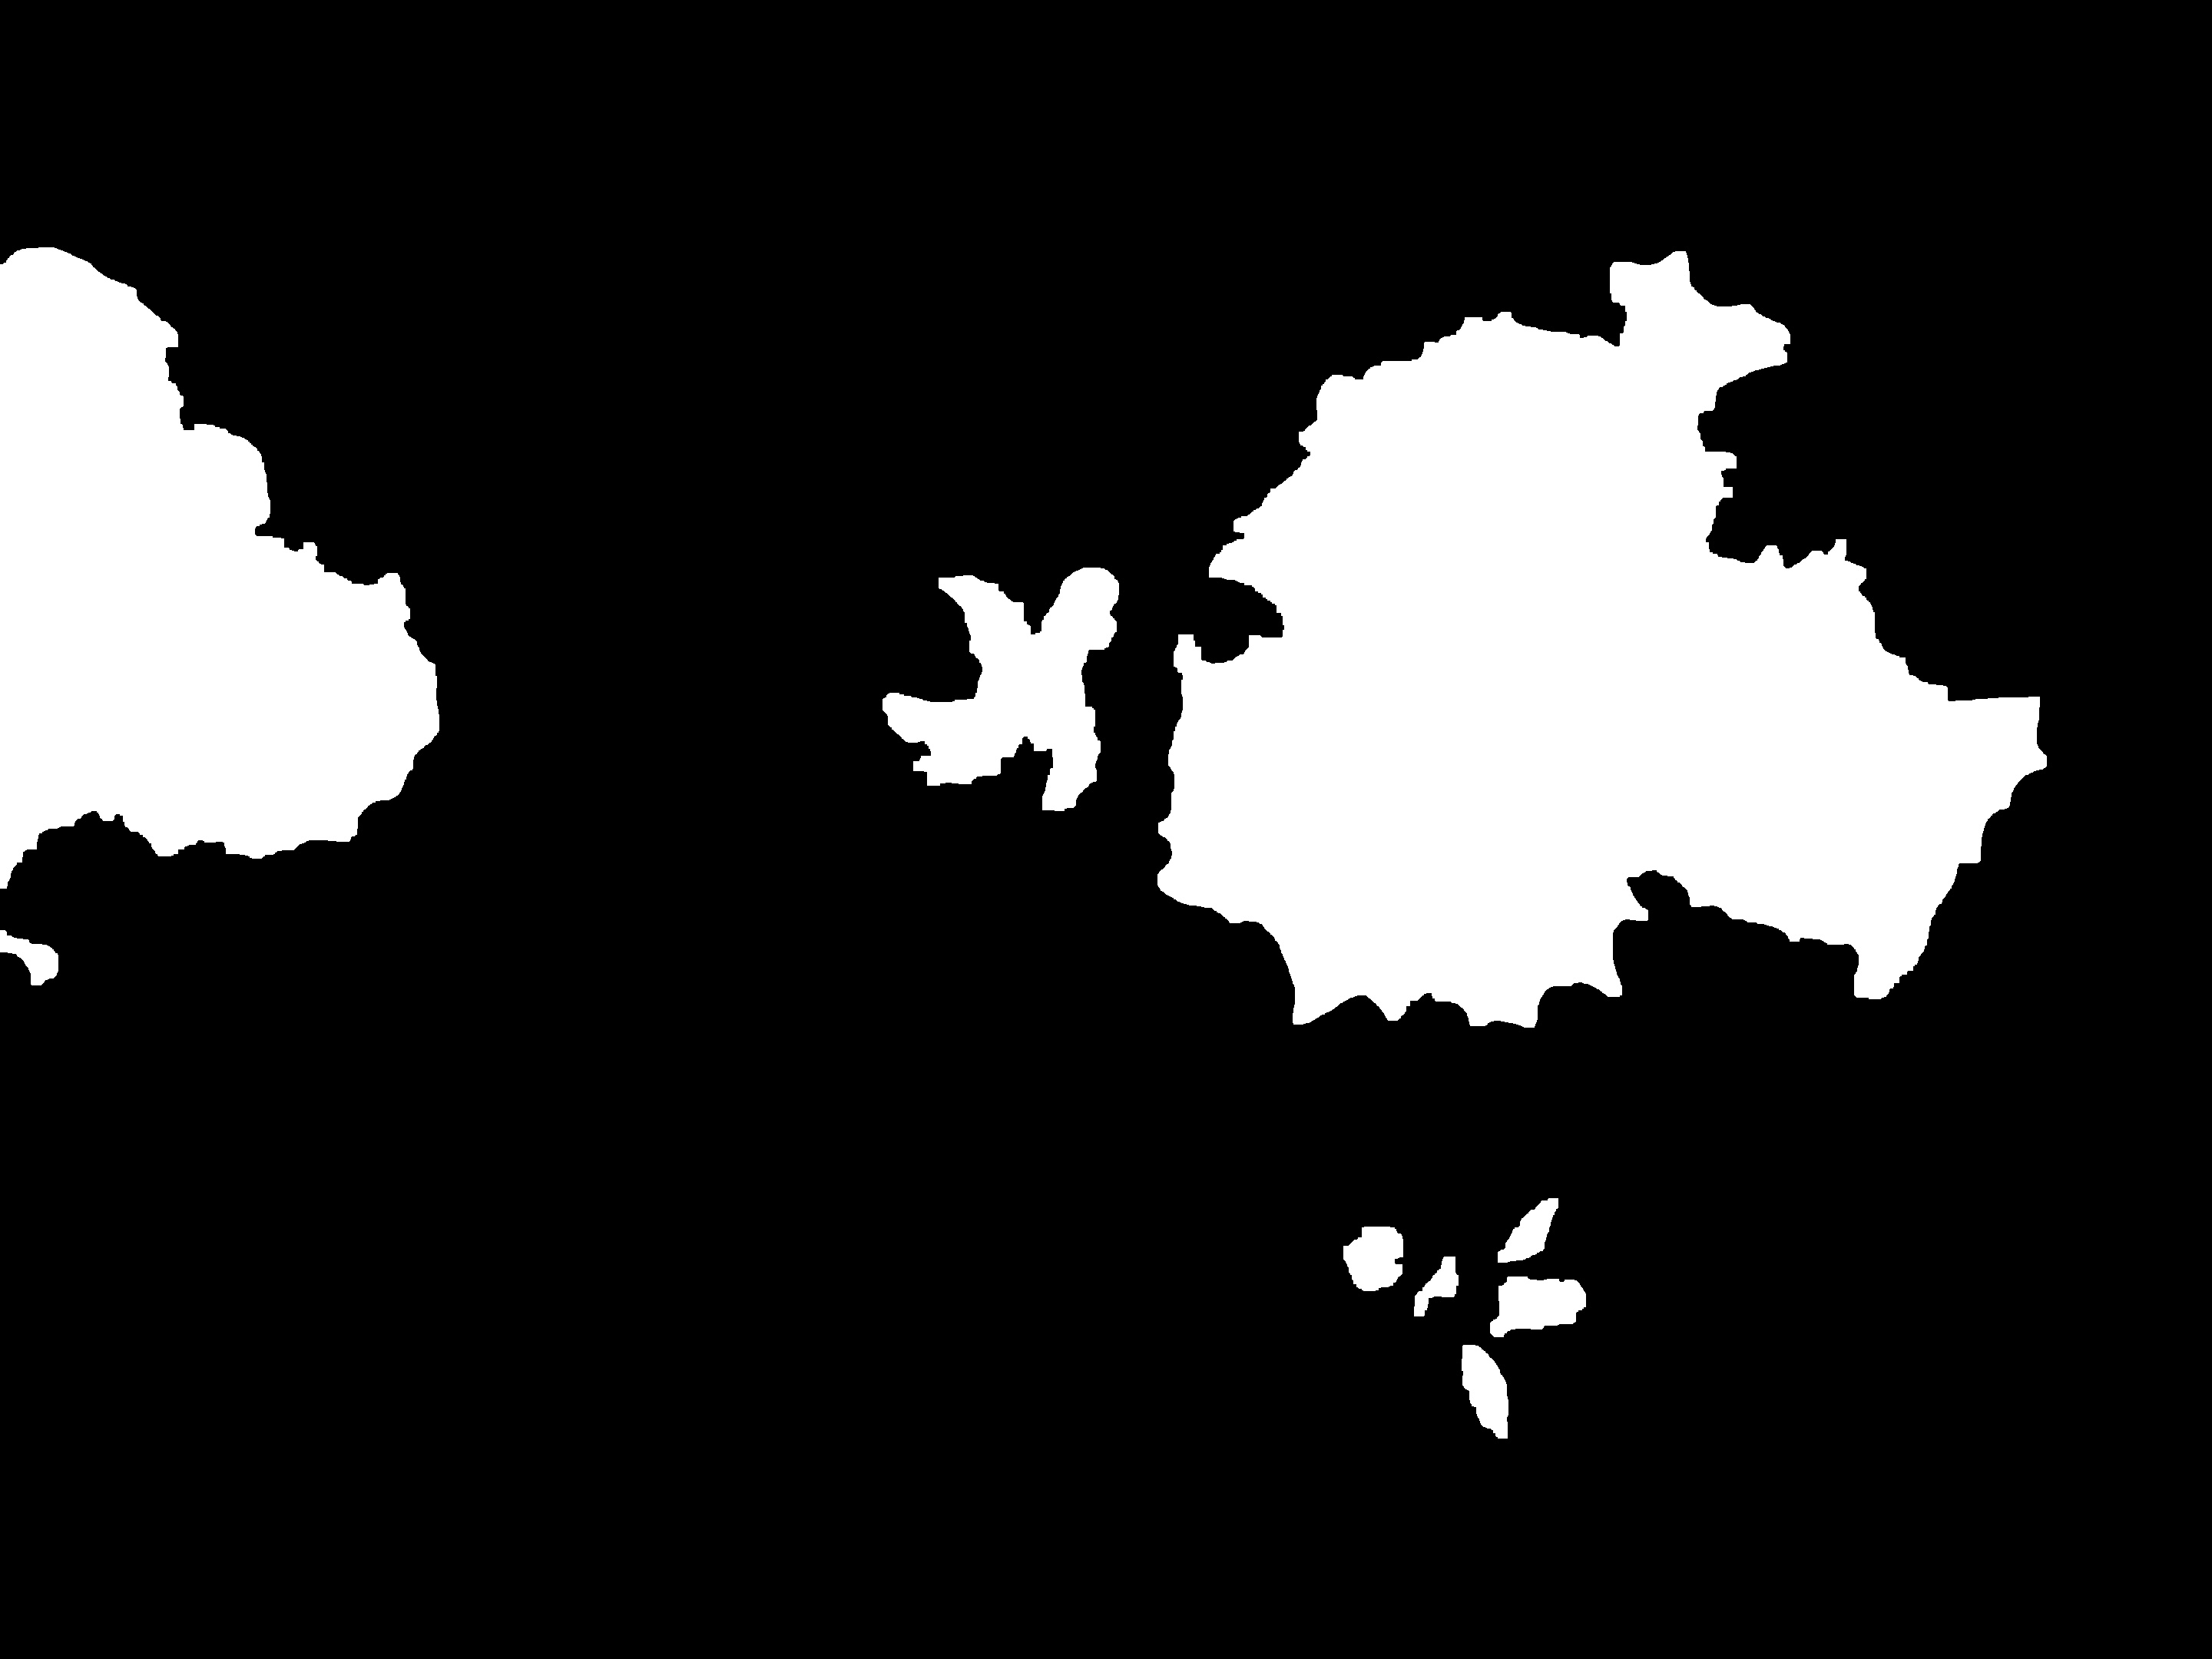
\includegraphics[width=1\linewidth]{figures/original-mask.jpg}
	  \caption{Mask produced with NDI}
	  \label{fig:mask}
	\end{subfigure}
	\begin{subfigure}[h]{.30\textwidth}
	  \centering
	  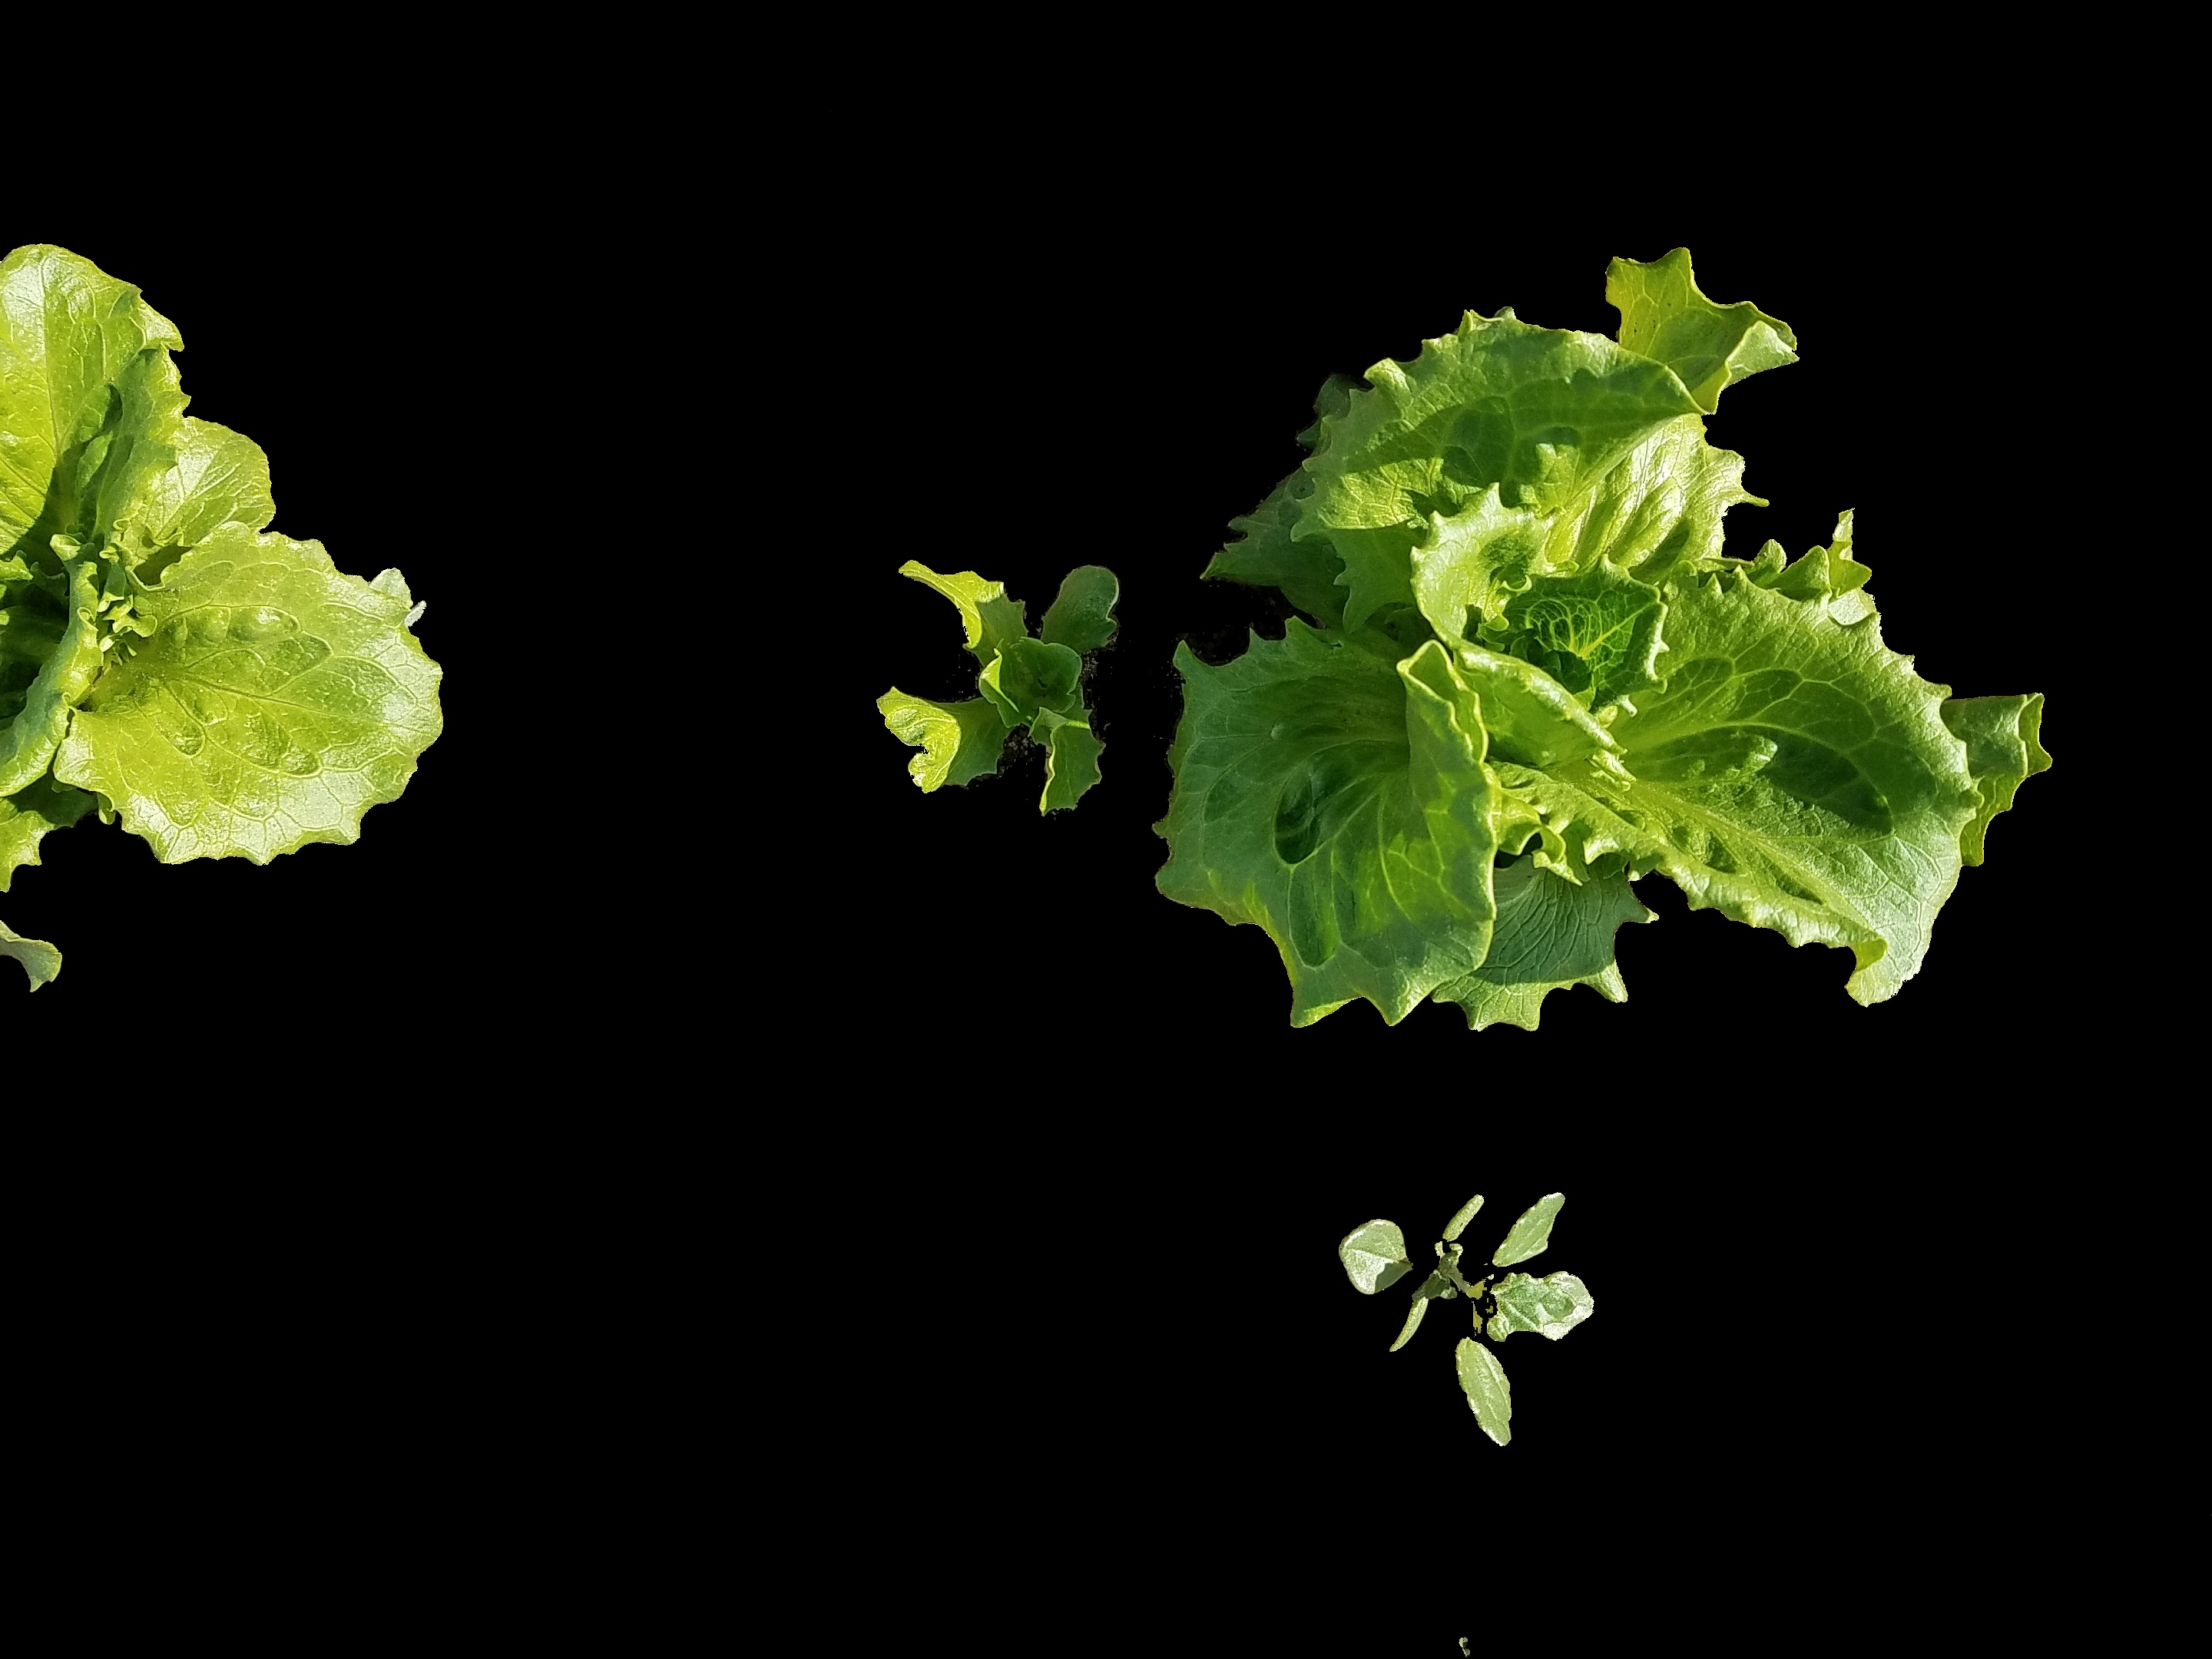
\includegraphics[width=1\linewidth]{figures/original-masked.jpg}
	  \caption{After applying mask}
	  \label{fig:original-masked}
	\end{subfigure}
	\caption[Before and after segmentation]{Before and after segmentation. Note the absence of the stems seen in the weed in the lower portion of~\ref{fig:original-masked} -- this is made a bit more obvious with a close examination of the mask shown in~\ref{fig:mask}. The lack of stems will lead to a single plant being identified as multiple plants, an error that will not affect factors that describe the interior of a leaf (such as texture), but will affect factors describing the plant as a whole (the shape). This will be discussed further in the section detailing problems (Section \ref{section:problems-color}).}
	\label{fig:segmentation}
\end{figure}
The segmented image has discarded ground pixels while retaining most of the pixels that will be used, but a close examination reveals that pixels in the stems of the weed are also eliminated, as they are less green than the rest of the plant. This effect is even more pronounced when segmenting images of weed that do not contain green stems as would be seen in the red stems seen in \textit{Portulaca oleracea} (Purslane). While they are not eliminated, pixels in the area of the deep shadows of the vegetation may affect attempts to classify objects based on color attributes. Unfortunately, the band of color featured in the stems (red) is frequently found in the background (soil), so attempts to make the stems appear in the masked image are problematic, as this solution tends to bring allow unwanted ground pixels in the final image that contain hues found within the stems. Likewise, immature vegetation where stems are not sufficiently green will not appear in the final image. 

The creation of an index exaggerates portions of the image with vegetated pixels. Deciding what portions of the data to discard based on these exaggerated values can be automated instead of using a single threshold for all images. The manual selection of a threshold can be shown to work relatively well, and can be fine-tuned by examining the results ensure that the number of vegetated pixels are maximized, while the number of non-vegetated pixels are minimized. Because images can be acquired under different lighting conditions, leading to the case where there is often not a single, effective threshold that works well for all images. An alternative, first proposed by \citeauthor{Otsu1979-io}, is to select this threshold automatically for each image \cite{Otsu1979-io}. Alternatively, the threshold for the image can be selected using the \textit{Triangle} algorithm.
Otsu’s Method is a histogram-based thresholding approach that automatically determines the optimal threshold by minimizing intra-class variance. It assumes that the image consists of two distinct classes—foreground and background—each represented by a bimodal histogram. The method iterates over all possible threshold values and selects the one that maximizes the variance between the two classes while minimizing the variance within each class.

 Otsu's algorithm arrives at a threshold by maximizing the variance between foreground and background pixels. The triangle method arrives at a threshold as the point where a line connecting the histogram’s peak to the maximum intensity is maximized. Both of these techniques operate on greyscale images, considering only pixel intensity. 
It is also worth considering the distribution of pixel values: bi-modal (two distinct peaks) and uni-modal (a single peak).

%
% Histogram produced with this command:'
% python plot-threshold.py -i d:\maricopa-test\flood-2-2m\DJI_0610.jpg

\begin{figure*}[h]
	\centering
	  	\subfloat[Intensity Histogram\centering]{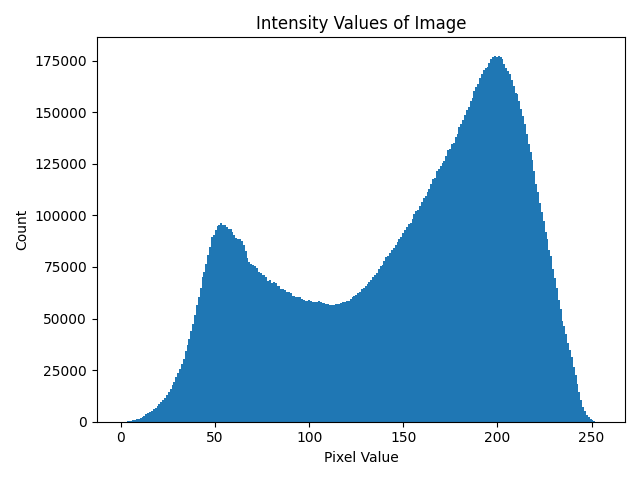
\includegraphics[height=0.19\textheight]{figures/pixel-values.png}\label{fig:intensity-histogram}}
		\hfil
	   	\subfloat[Source Image\centering]{\includegraphics[height=0.19\textheight]{figures/pixel-values-image.jpg}
	  \label{fig:source-image}}
	\caption[Bimodal distribution of pixel intensity]{An example of a bimodal distribution of pixel intensity values. Note that there are two peaks in the histogram above (\ref{fig:intensity-histogram}), corresponding to the two classes in \ref{fig:source-image}: crop and ground.}
	\label{fig:intensity}
\end{figure*}

Otsu's method operates on the assumption that there are two classes of pixels in the object (interesting and uninteresting things). The algorithm minimizes intra-class variance. This method performs well when presented with images that have two distinct peaks.

% Equation from https://infoaryan.com/blog/opencv-python-otsu-and-triangle-thresholding-full-mathematics-code-explained-important/
\begin{equation}
\sigma^2_B (t) \times p(t) \times p(\overline{t}) \\
\end{equation}
where $\sigma^2_B (t)$ is the variance between the two classes, $p(t)$ is the probability of class $t$, and $p(\overline{t})$ is the probability of the complement.

The Triangle Method is another automatic thresholding approach that is particularly effective when dealing with unimodal histograms. Instead of assuming a bimodal distribution, this method determines a threshold by drawing a straight line from the peak of the histogram (the most frequent intensity) to the minimum intensity value on the histogram’s tail. The threshold is set at the point where the perpendicular distance between the line and the histogram is maximized.
\begin{equation}
T_{triangle} = argmax \left[ h(T) \times \left( 1 - \left| \frac{T - P}{R - P} \right| \right) \right]
\end{equation}
Where $h(T)$ is the value at $T$, $R$ is the maximum of the intensity, and $P$ is the peak value. The triangle method often performs better than does Otsu's method when the pixel intensities exhibit a unimodal peak.

The details of the implementation of these two approaches are beyond the scope of this work, and while there are certainly others, these are the most frequently proposed approaches. Both of these approaches, however, are based on some assumptions about the intensity histogram, and may not work well in all situations, particularly if these assumptions are not valid. Otsu's algorithm, for example, tends to yield satisfactory results when operating on images possessing a bimodal distribution, but may not yield good results on images with a single peak or multiple peaks.

\begin{figure}[h!]
	\centering
	\begin{subfigure}[h]{.48\textwidth}
	  \centering
	  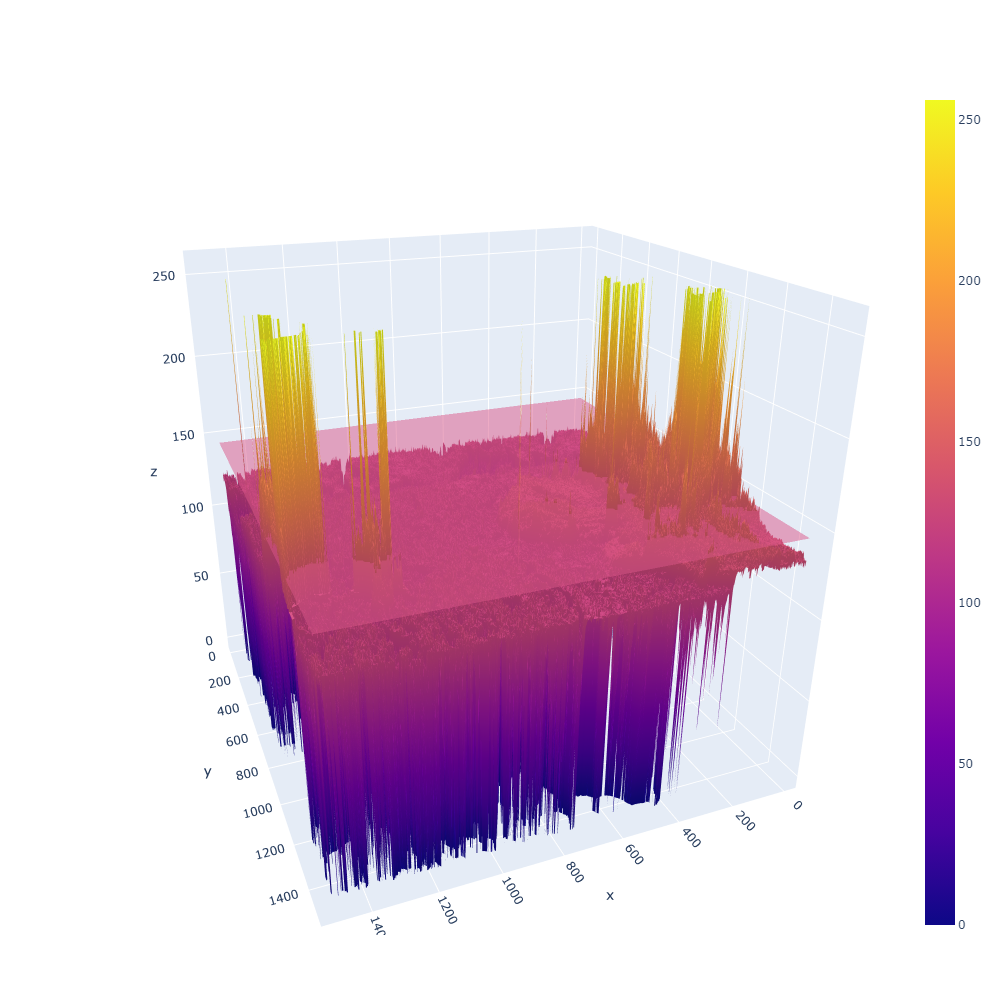
\includegraphics[height=5cm]{./figures/ndi-1-of-2.png}
	  \caption{Image segmented using NDI}
	  \label{fig:ndi-1}
	\end{subfigure}
	\hfil
	\begin{subfigure}[h]{.48\textwidth}
	  \centering
	  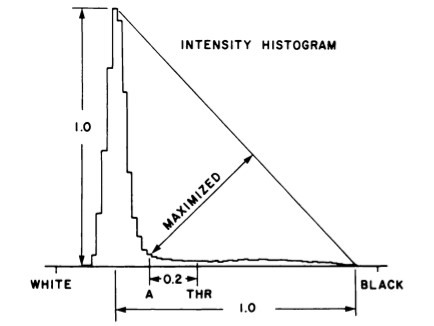
\includegraphics[height=5cm]{./figures/triangle-algorithm}
	  \caption{Triangle method for threshold selection.}
	  \label{fig:ndi-2}
	\end{subfigure}
	\caption[NDI segmentation and threshold selection]{An example of NDI segmentation and threshold selection. A threshold for the production of a mask can be done manually,  by selecting all values below 140 to form the mask that will be applied to the image, illustrated by the semi-opaque plane. While manual selection may be sufficient to perform the segmentation of an image set acquired under the same ambient conditions, it may lead to the exclusion of portions of the plant in images taken under different conditions. Using the \textit{Triangle} algorithm \parencite{Brink1996-xy,Zack1977-yl} allows this selection to be made automatically. The point at which the line between the lowest and highest points in the histogram is selected as the threshold, selecting a threshold applicable to each image in a set rather than a global value used for all images in a set.}
	\label{fig:ndi-segmentation}
\end{figure}

RGB based indices have a distinct advantage over other segmentation techniques for one very important reason: they are computationally cheap. While they involve as many calculations as there are pixels in the image, the number is relatively small. Given that compute resources may be limited in real-time systems operating under field conditions, this aspect may be an important factor worthy of consideration, particularly when a CPU is not dedicated to the imaging system. While the index calculation may benefit from the use of  a GPU, a detailed analysis of the benefit of doing so is discussed in the section on performance (Section \ref{section:performance}).

Figure \ref{figure:results} shows the results of applying the masks to a image containing both ground and vegetation.

\begin{figure}[H]
\centering
\captionsetup[subfloat]{labelfont=scriptsize,textfont=scriptsize}
\begin{tabular}{cccccc}
\subfloat[NDI]{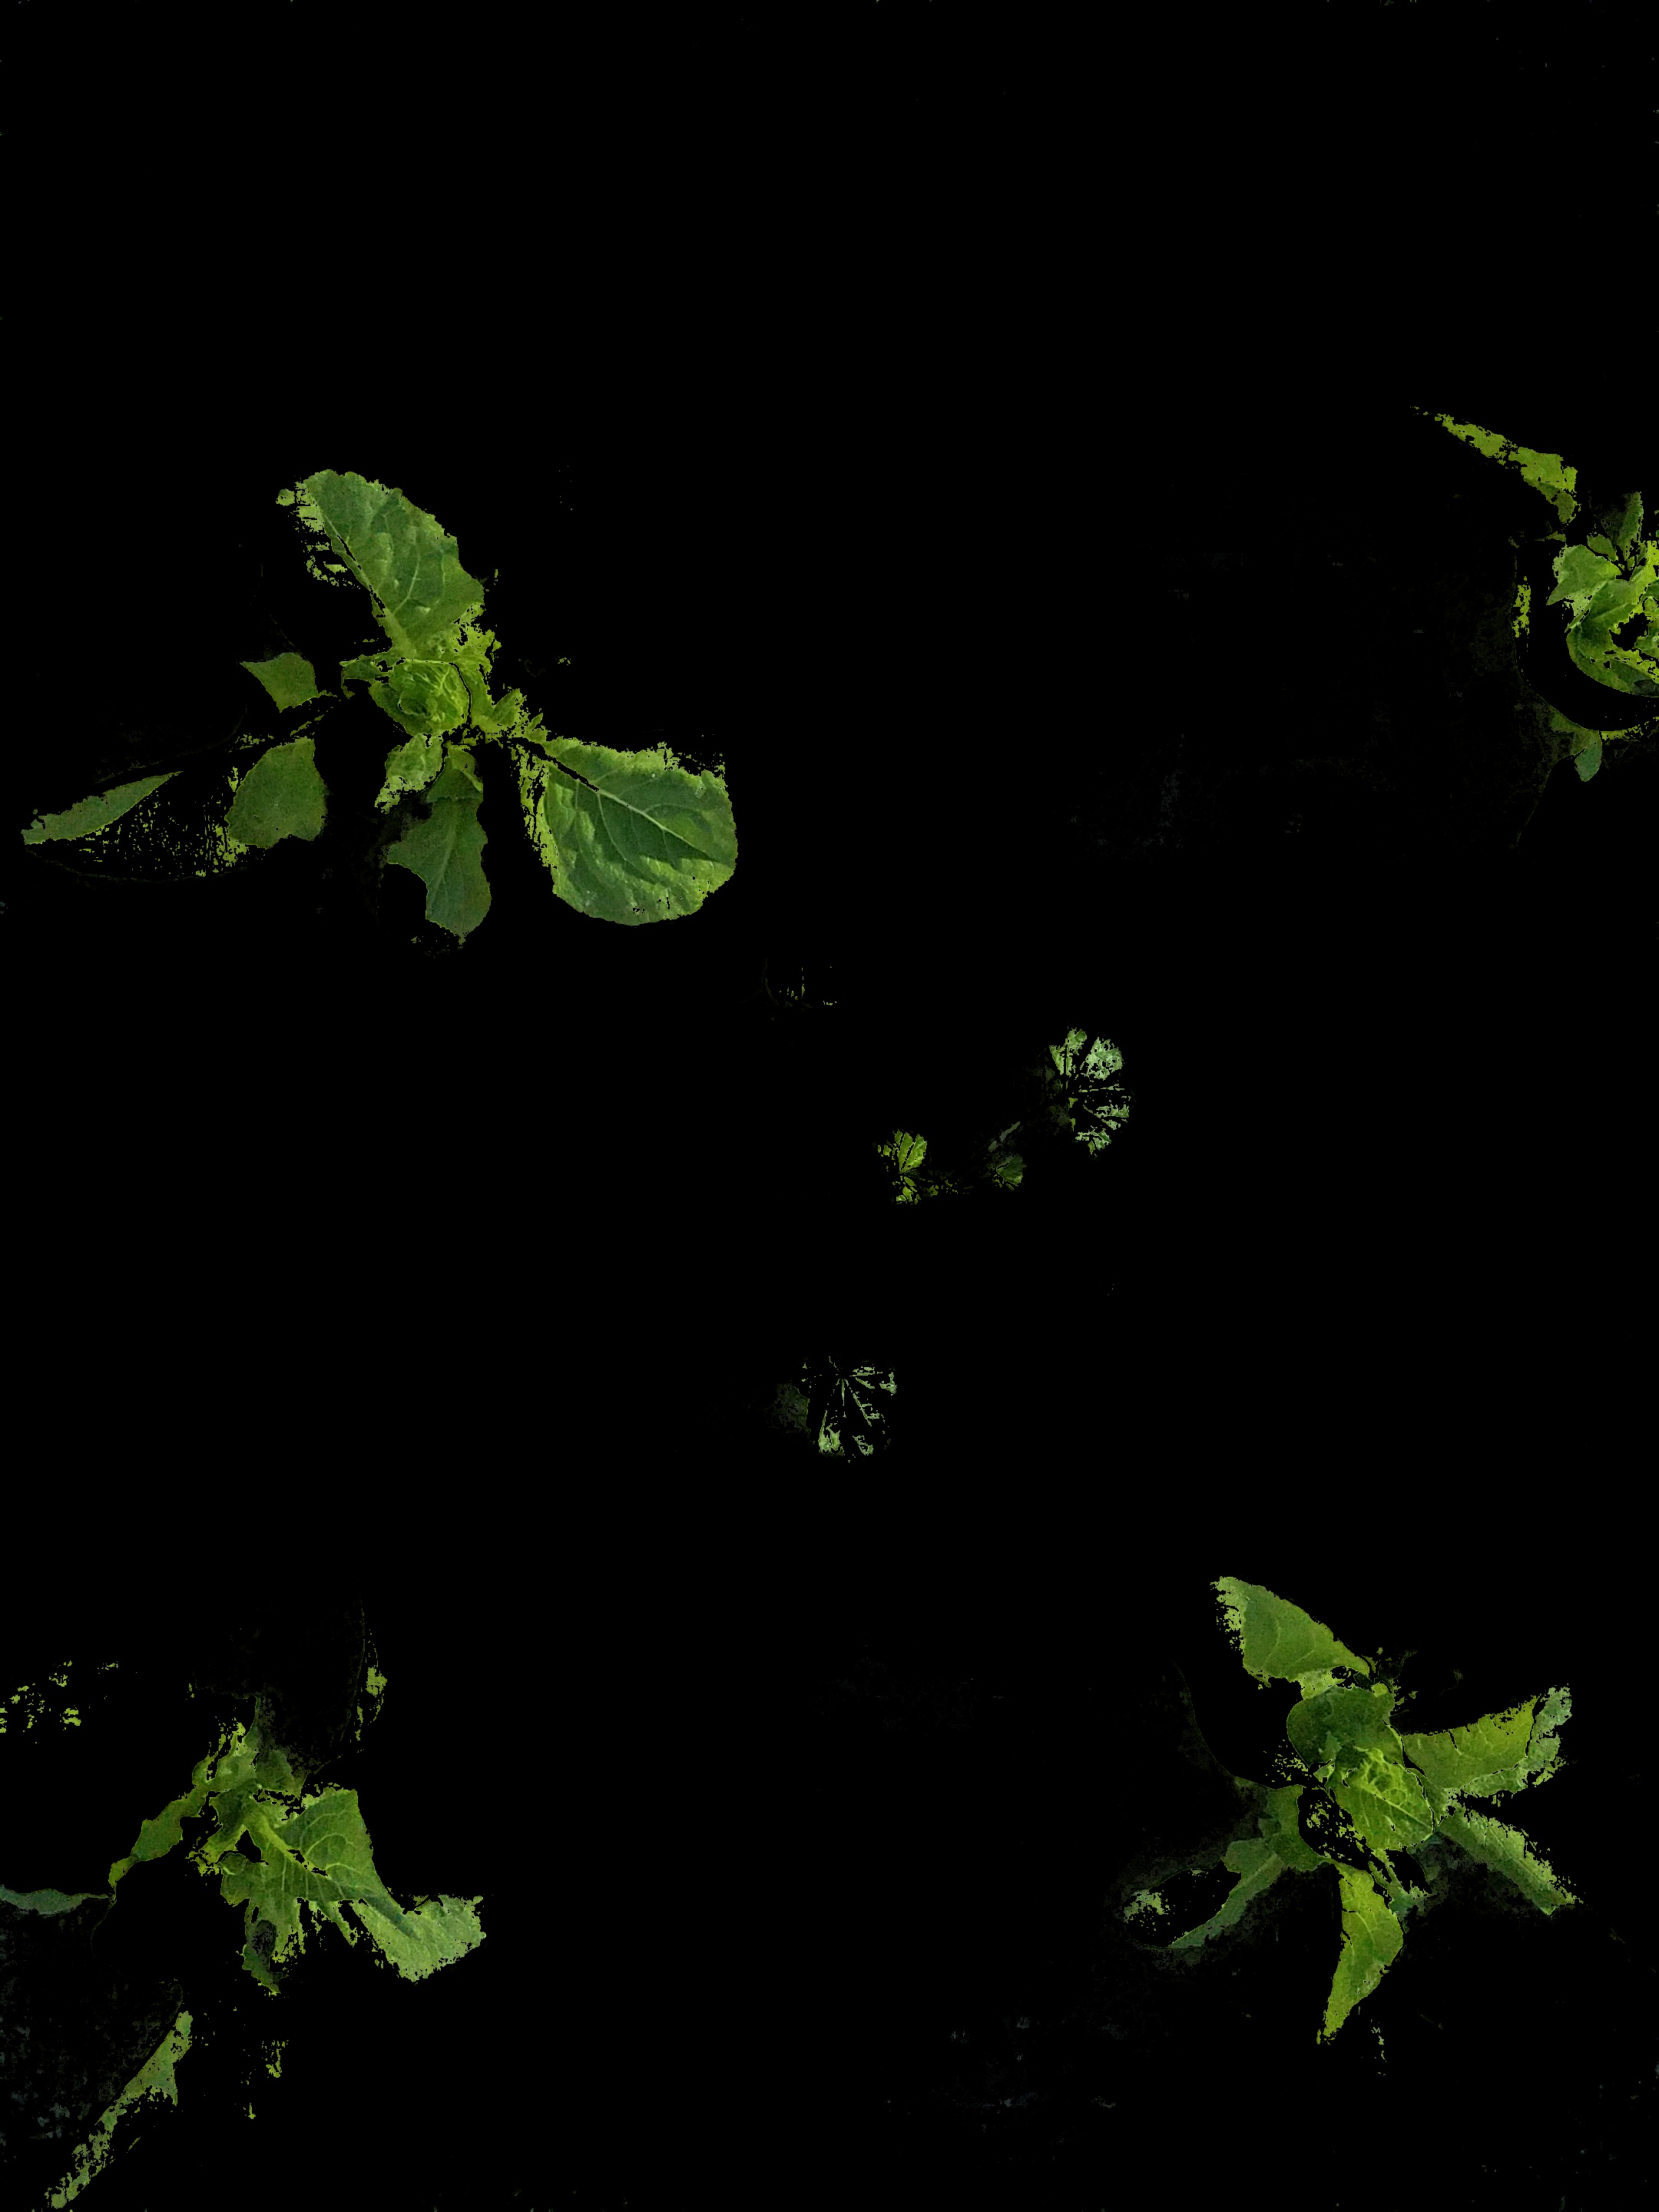
\includegraphics[height=0.10\textheight]{figures/20201117_112624-NDI.jpg} \label{fig:ndi}} &
\subfloat[EXG]{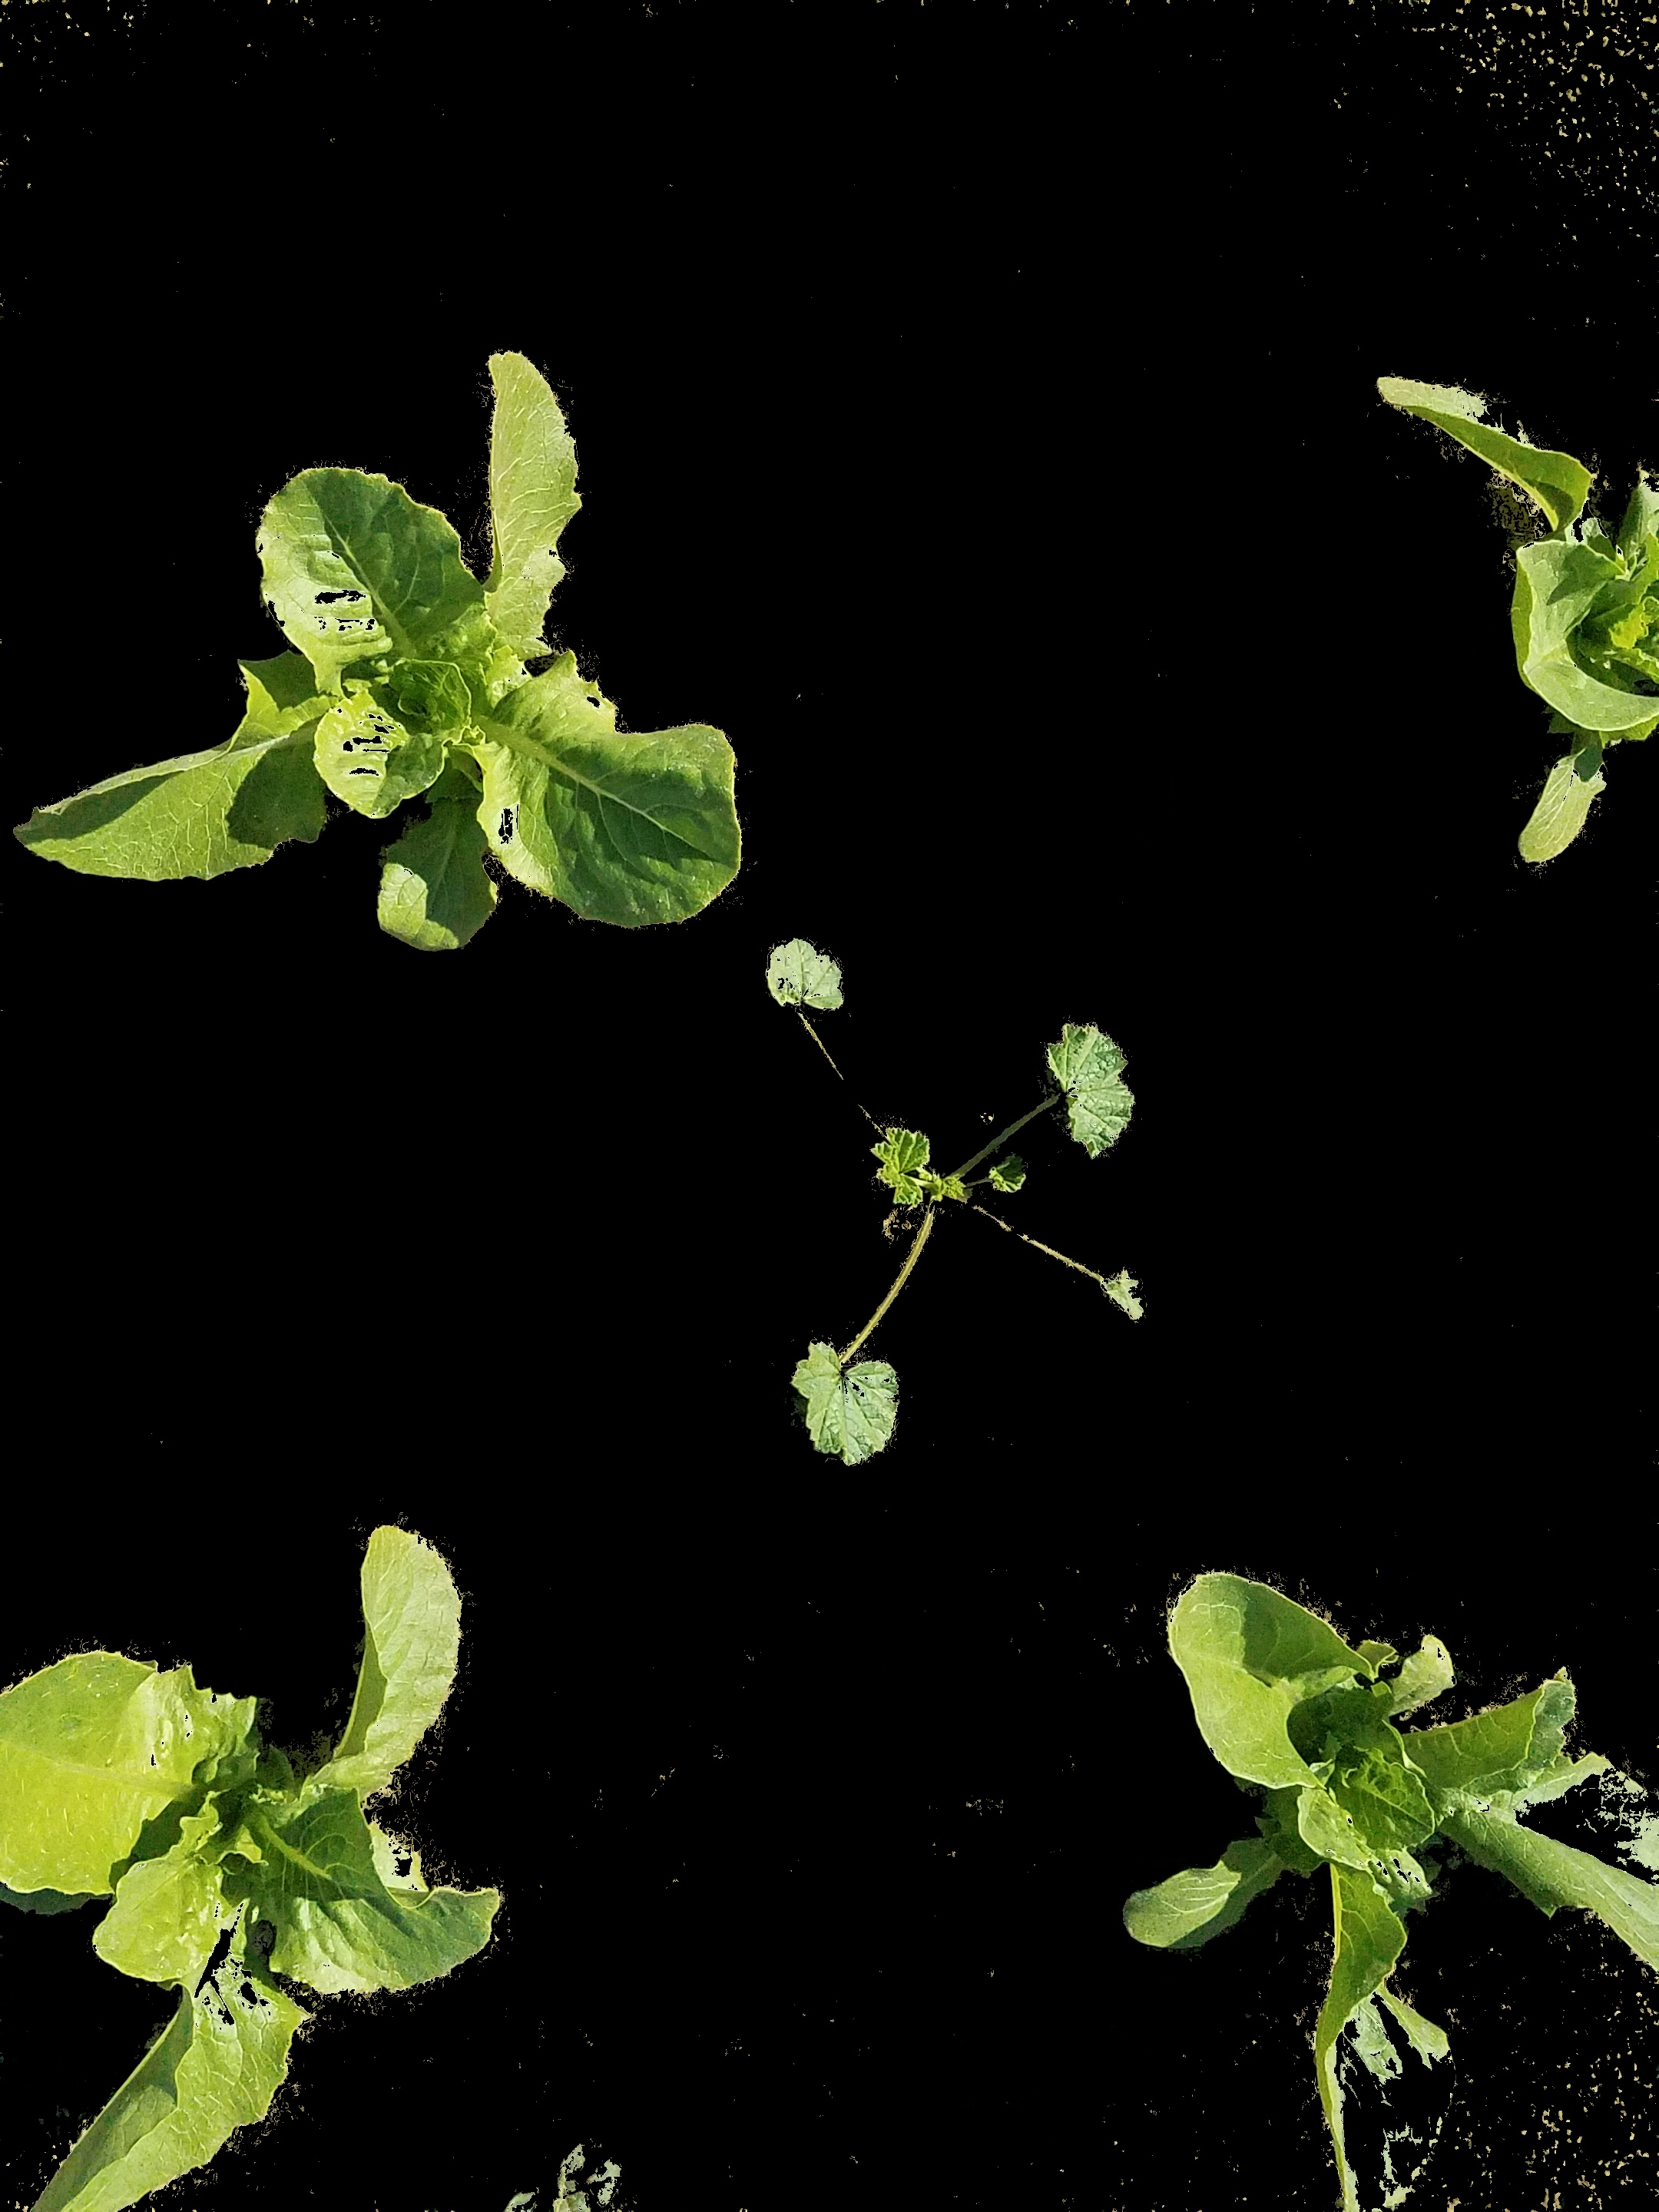
\includegraphics[height=0.10\textheight]{figures/20201117_112624-ExG.jpg} \label{fig:exg}} &
\subfloat[EXR]{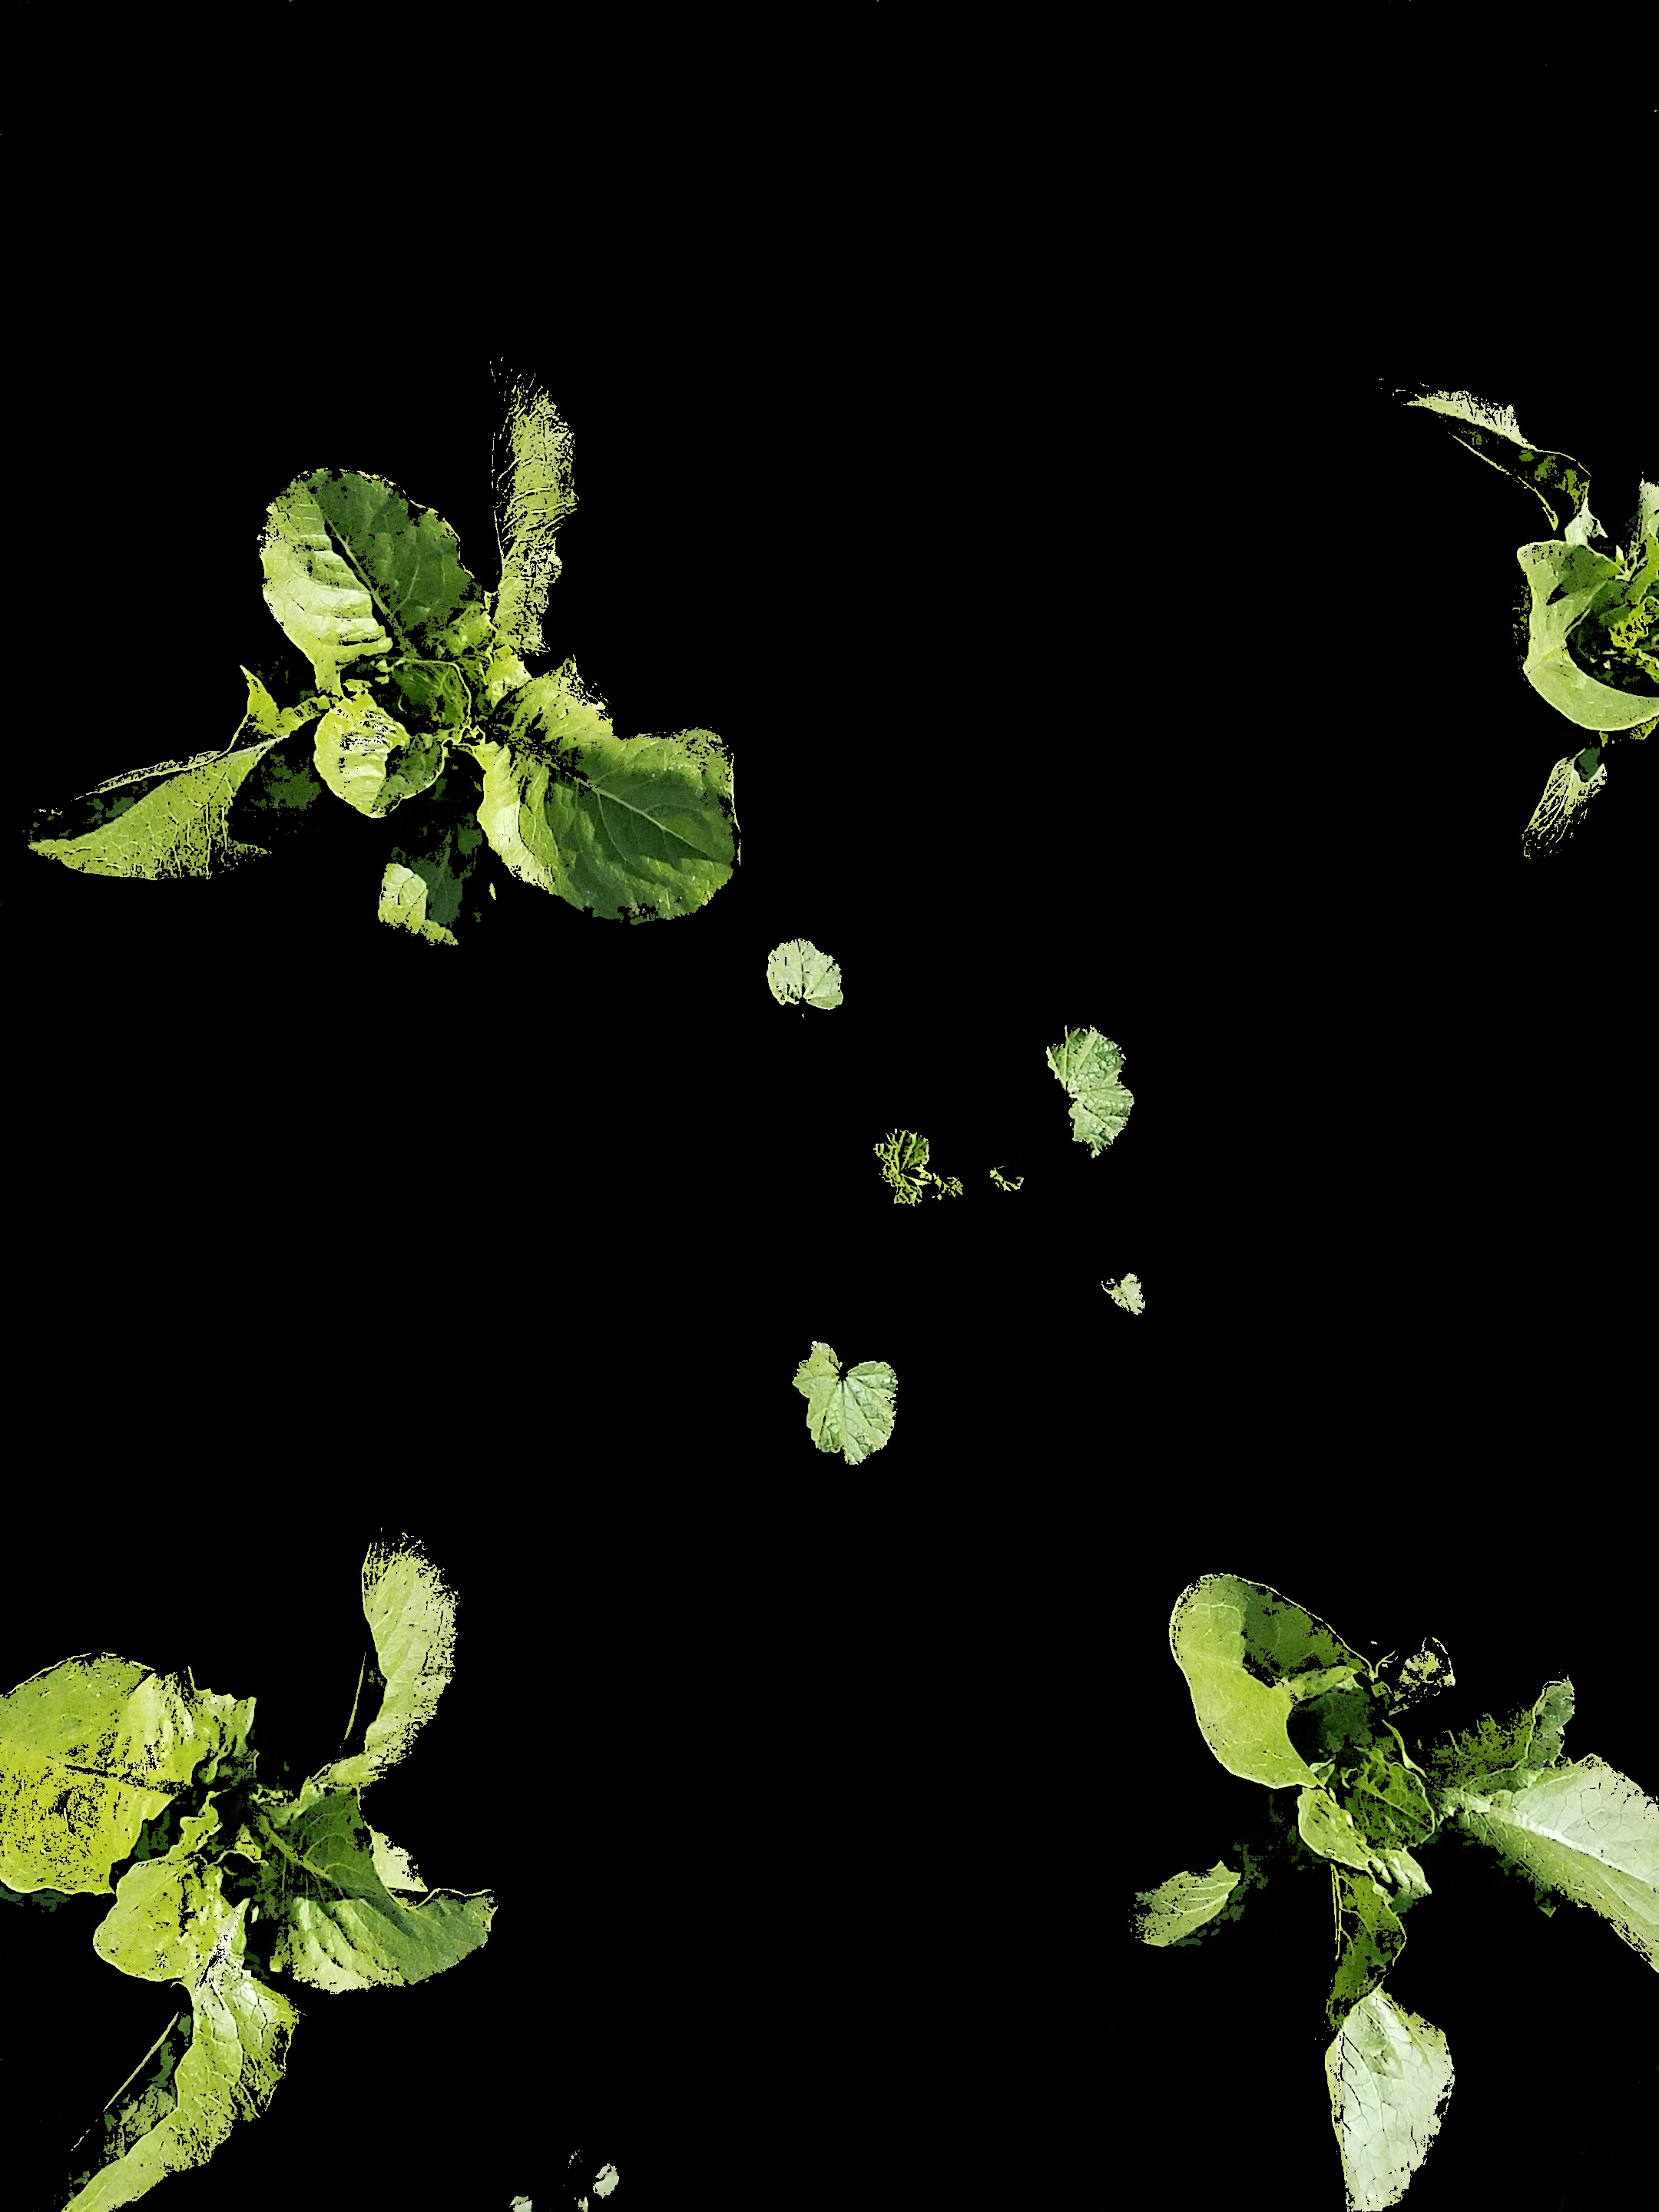
\includegraphics[height=0.10\textheight]{figures/20201117_112624-ExR.jpg} \label{fig:exr}} &
\subfloat[CIVE]{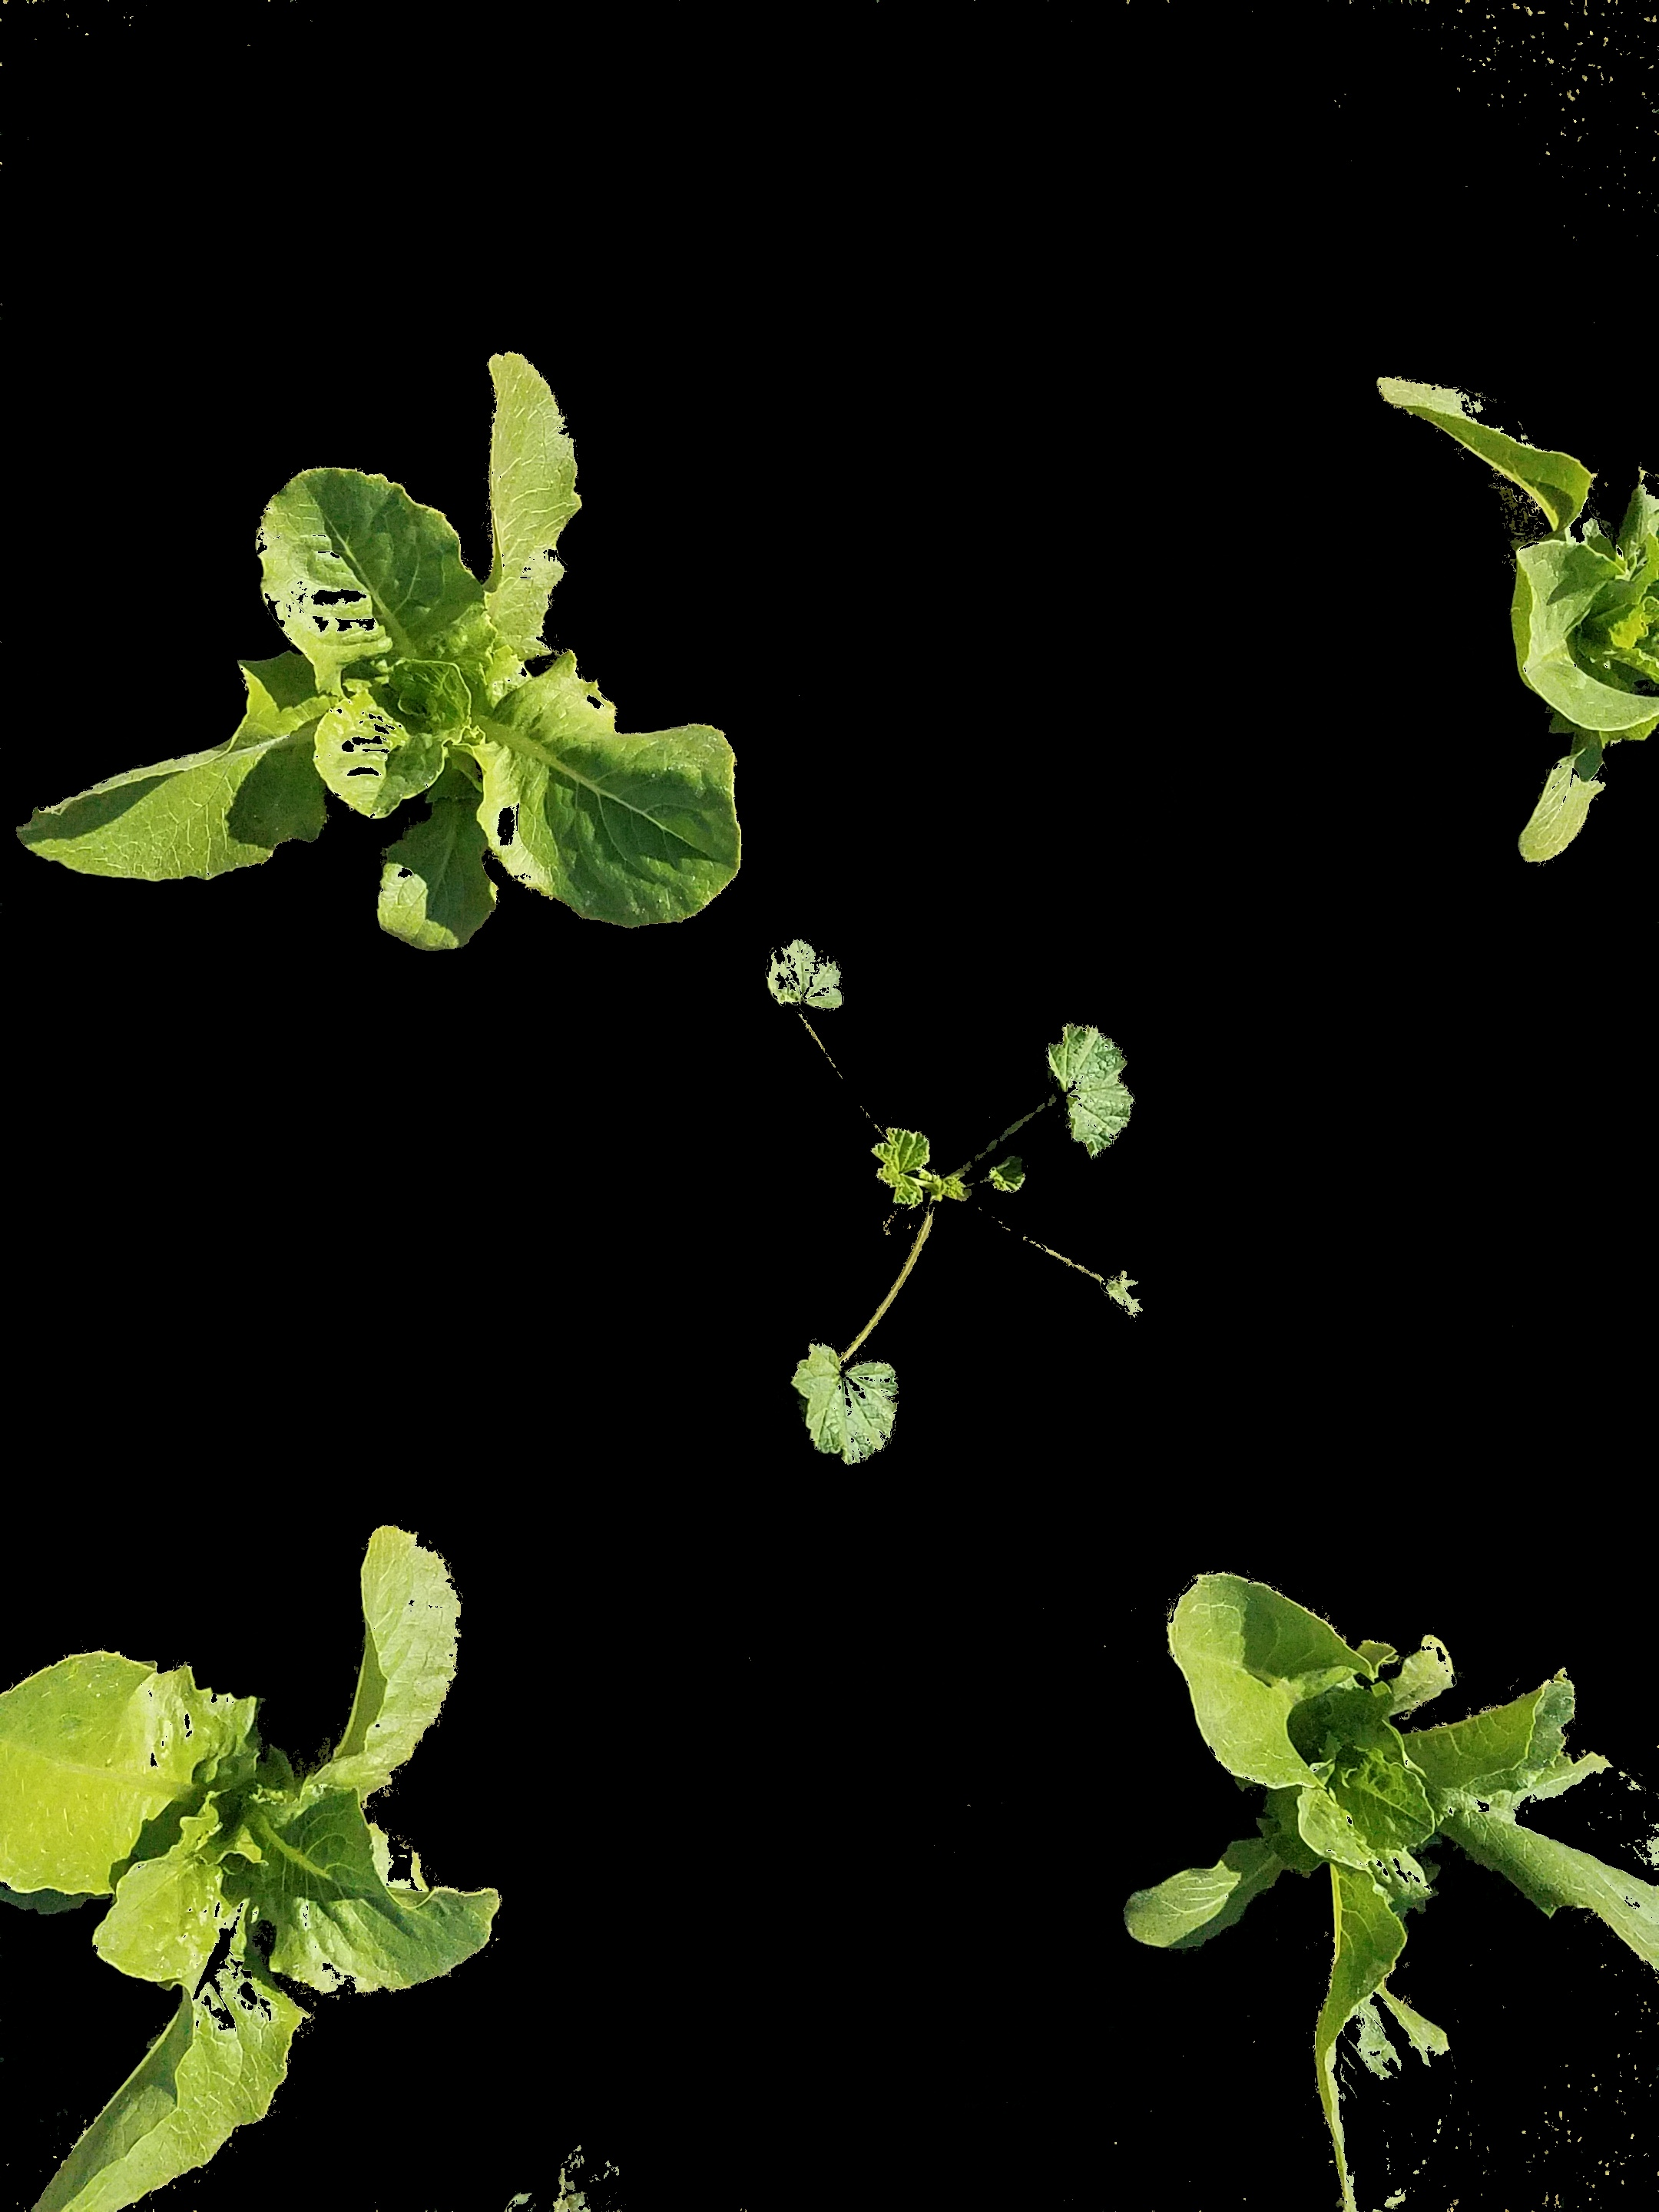
\includegraphics[height=0.10\textheight]{figures/20201117_112624-CIVE.jpg} \label{fig:cive}} &
\subfloat[EXG-EXR]{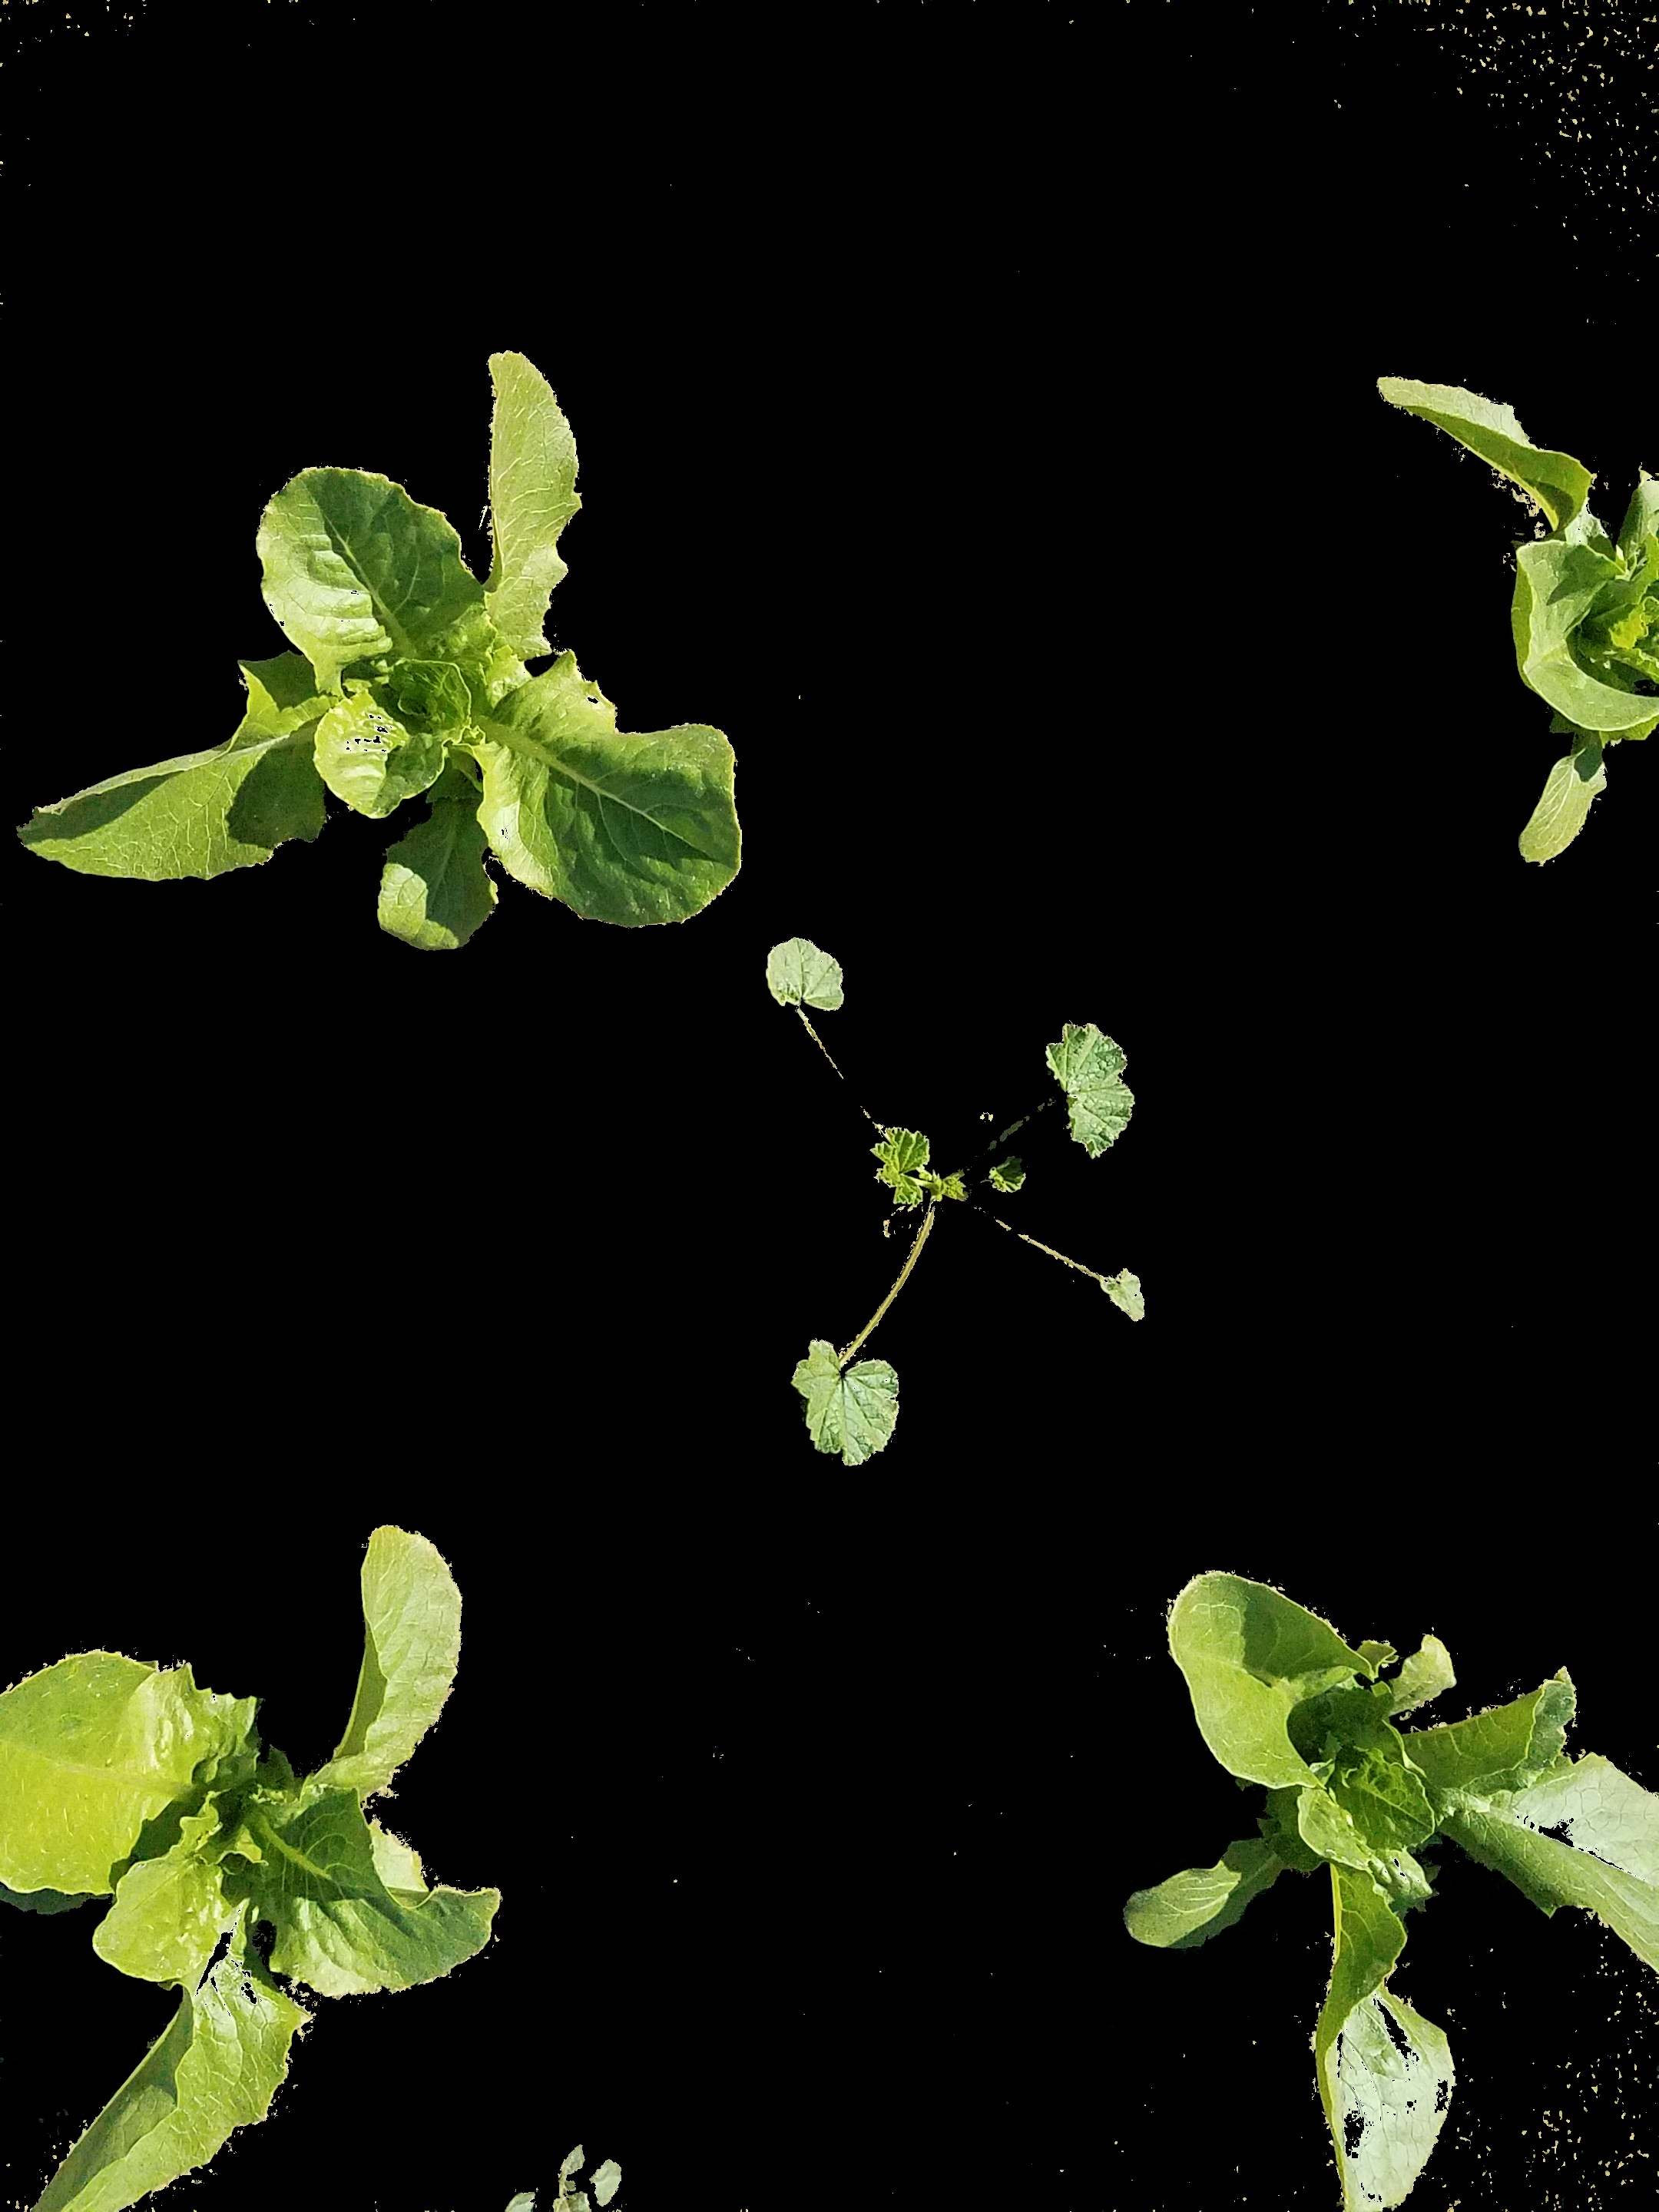
\includegraphics[height=0.10\textheight]{figures/20201117_112624-ExGR.jpg} \label{fig:exgexr}} &
\subfloat[NGRDI]{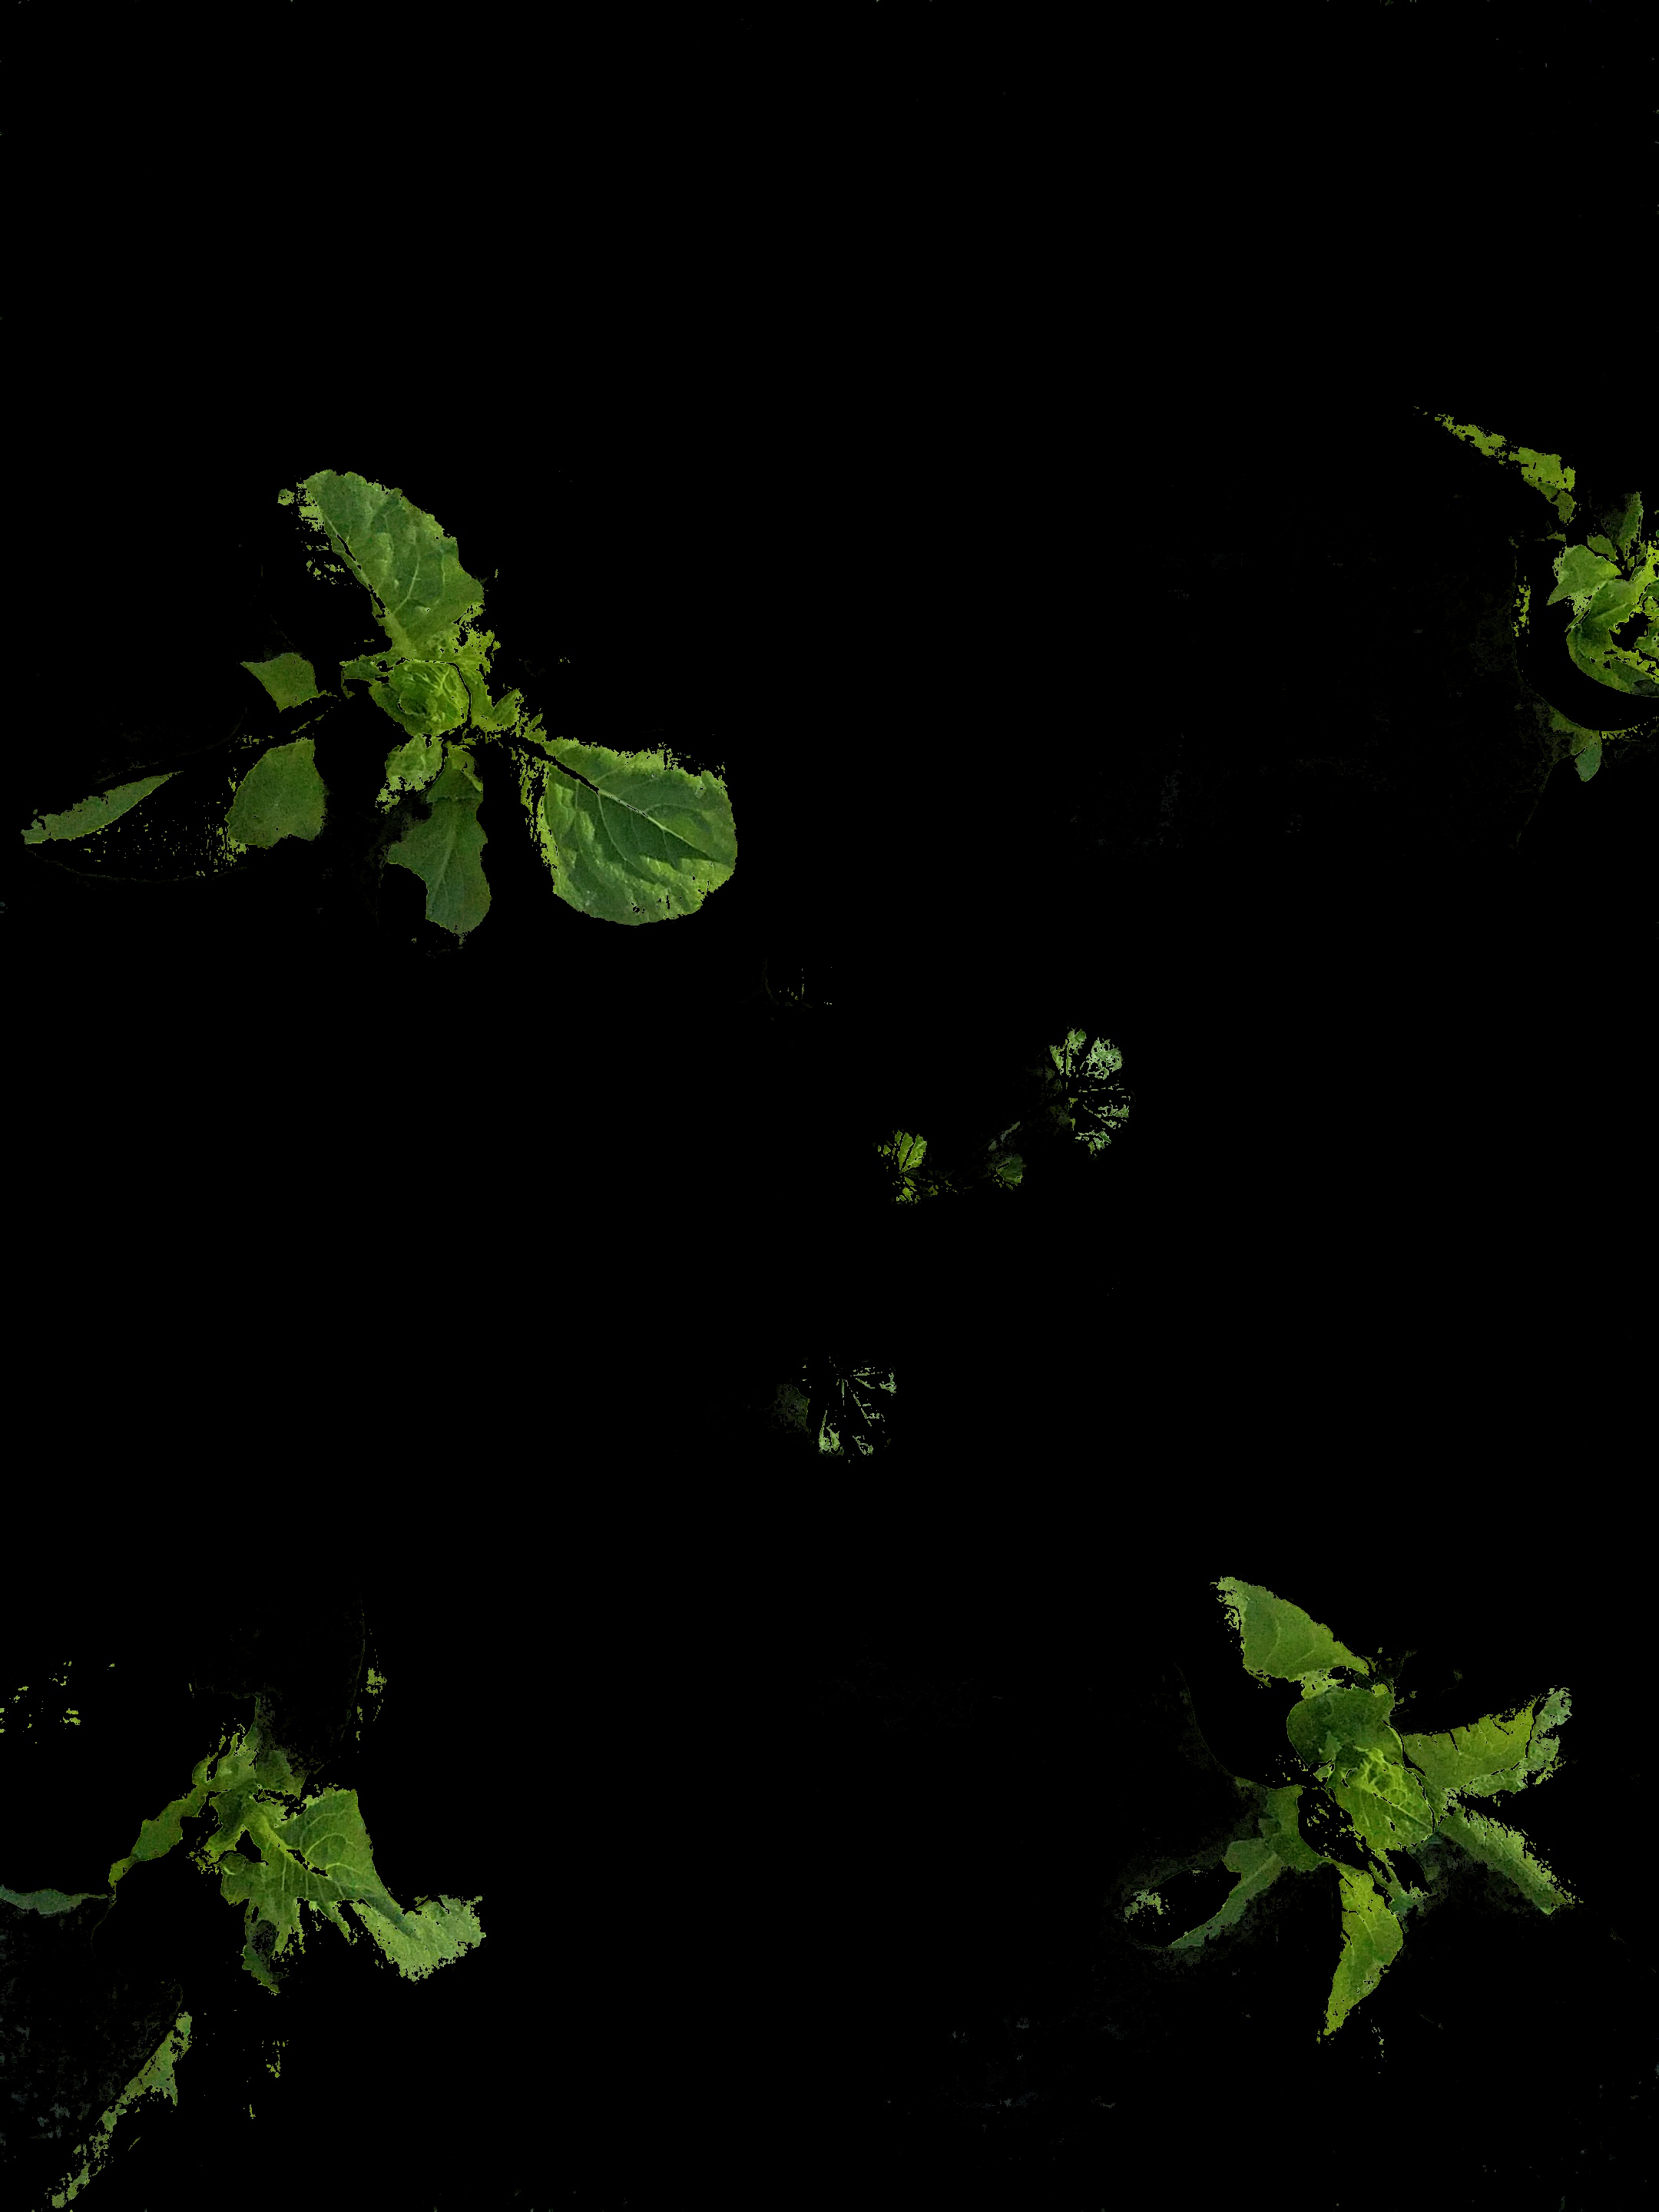
\includegraphics[height=0.10\textheight]{figures/20201117_112624-NGRDI.jpg} \label{fig:nrgdi}} \\
\subfloat[Com1]{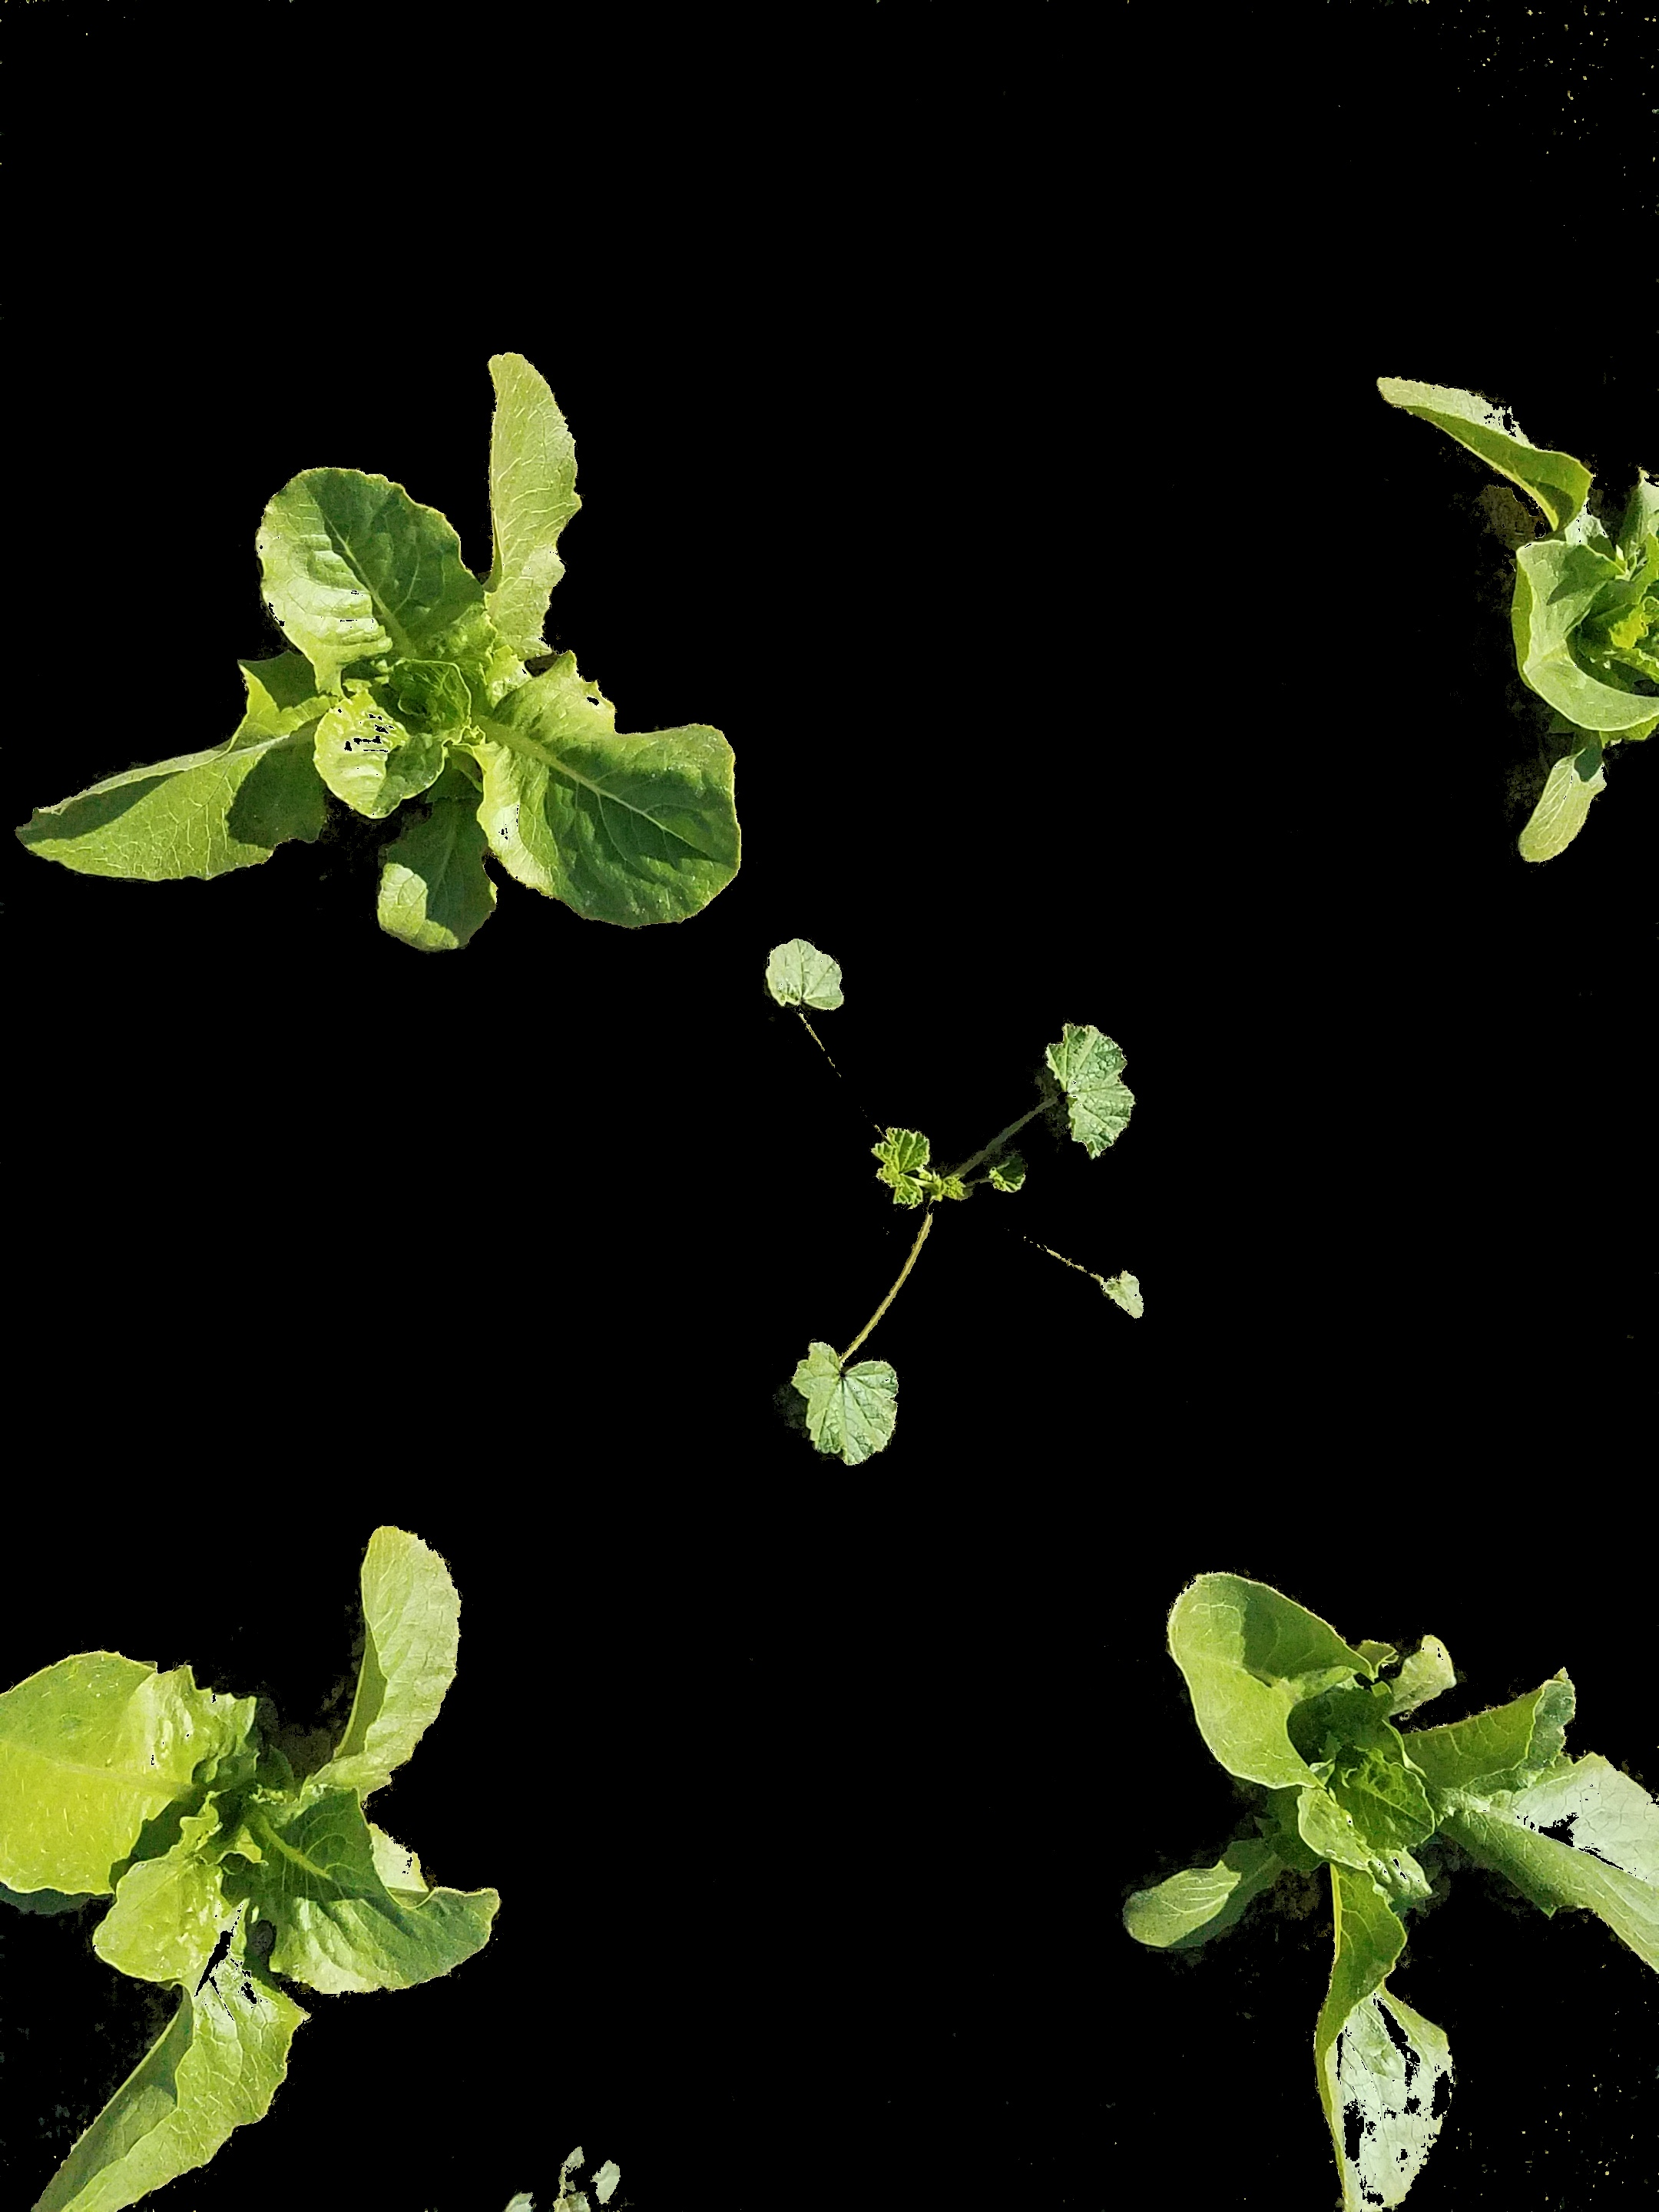
\includegraphics[height=0.10\textheight]{figures/20201117_112624-COM1.jpg} \label{fig:com1}} &
\subfloat[Com2]{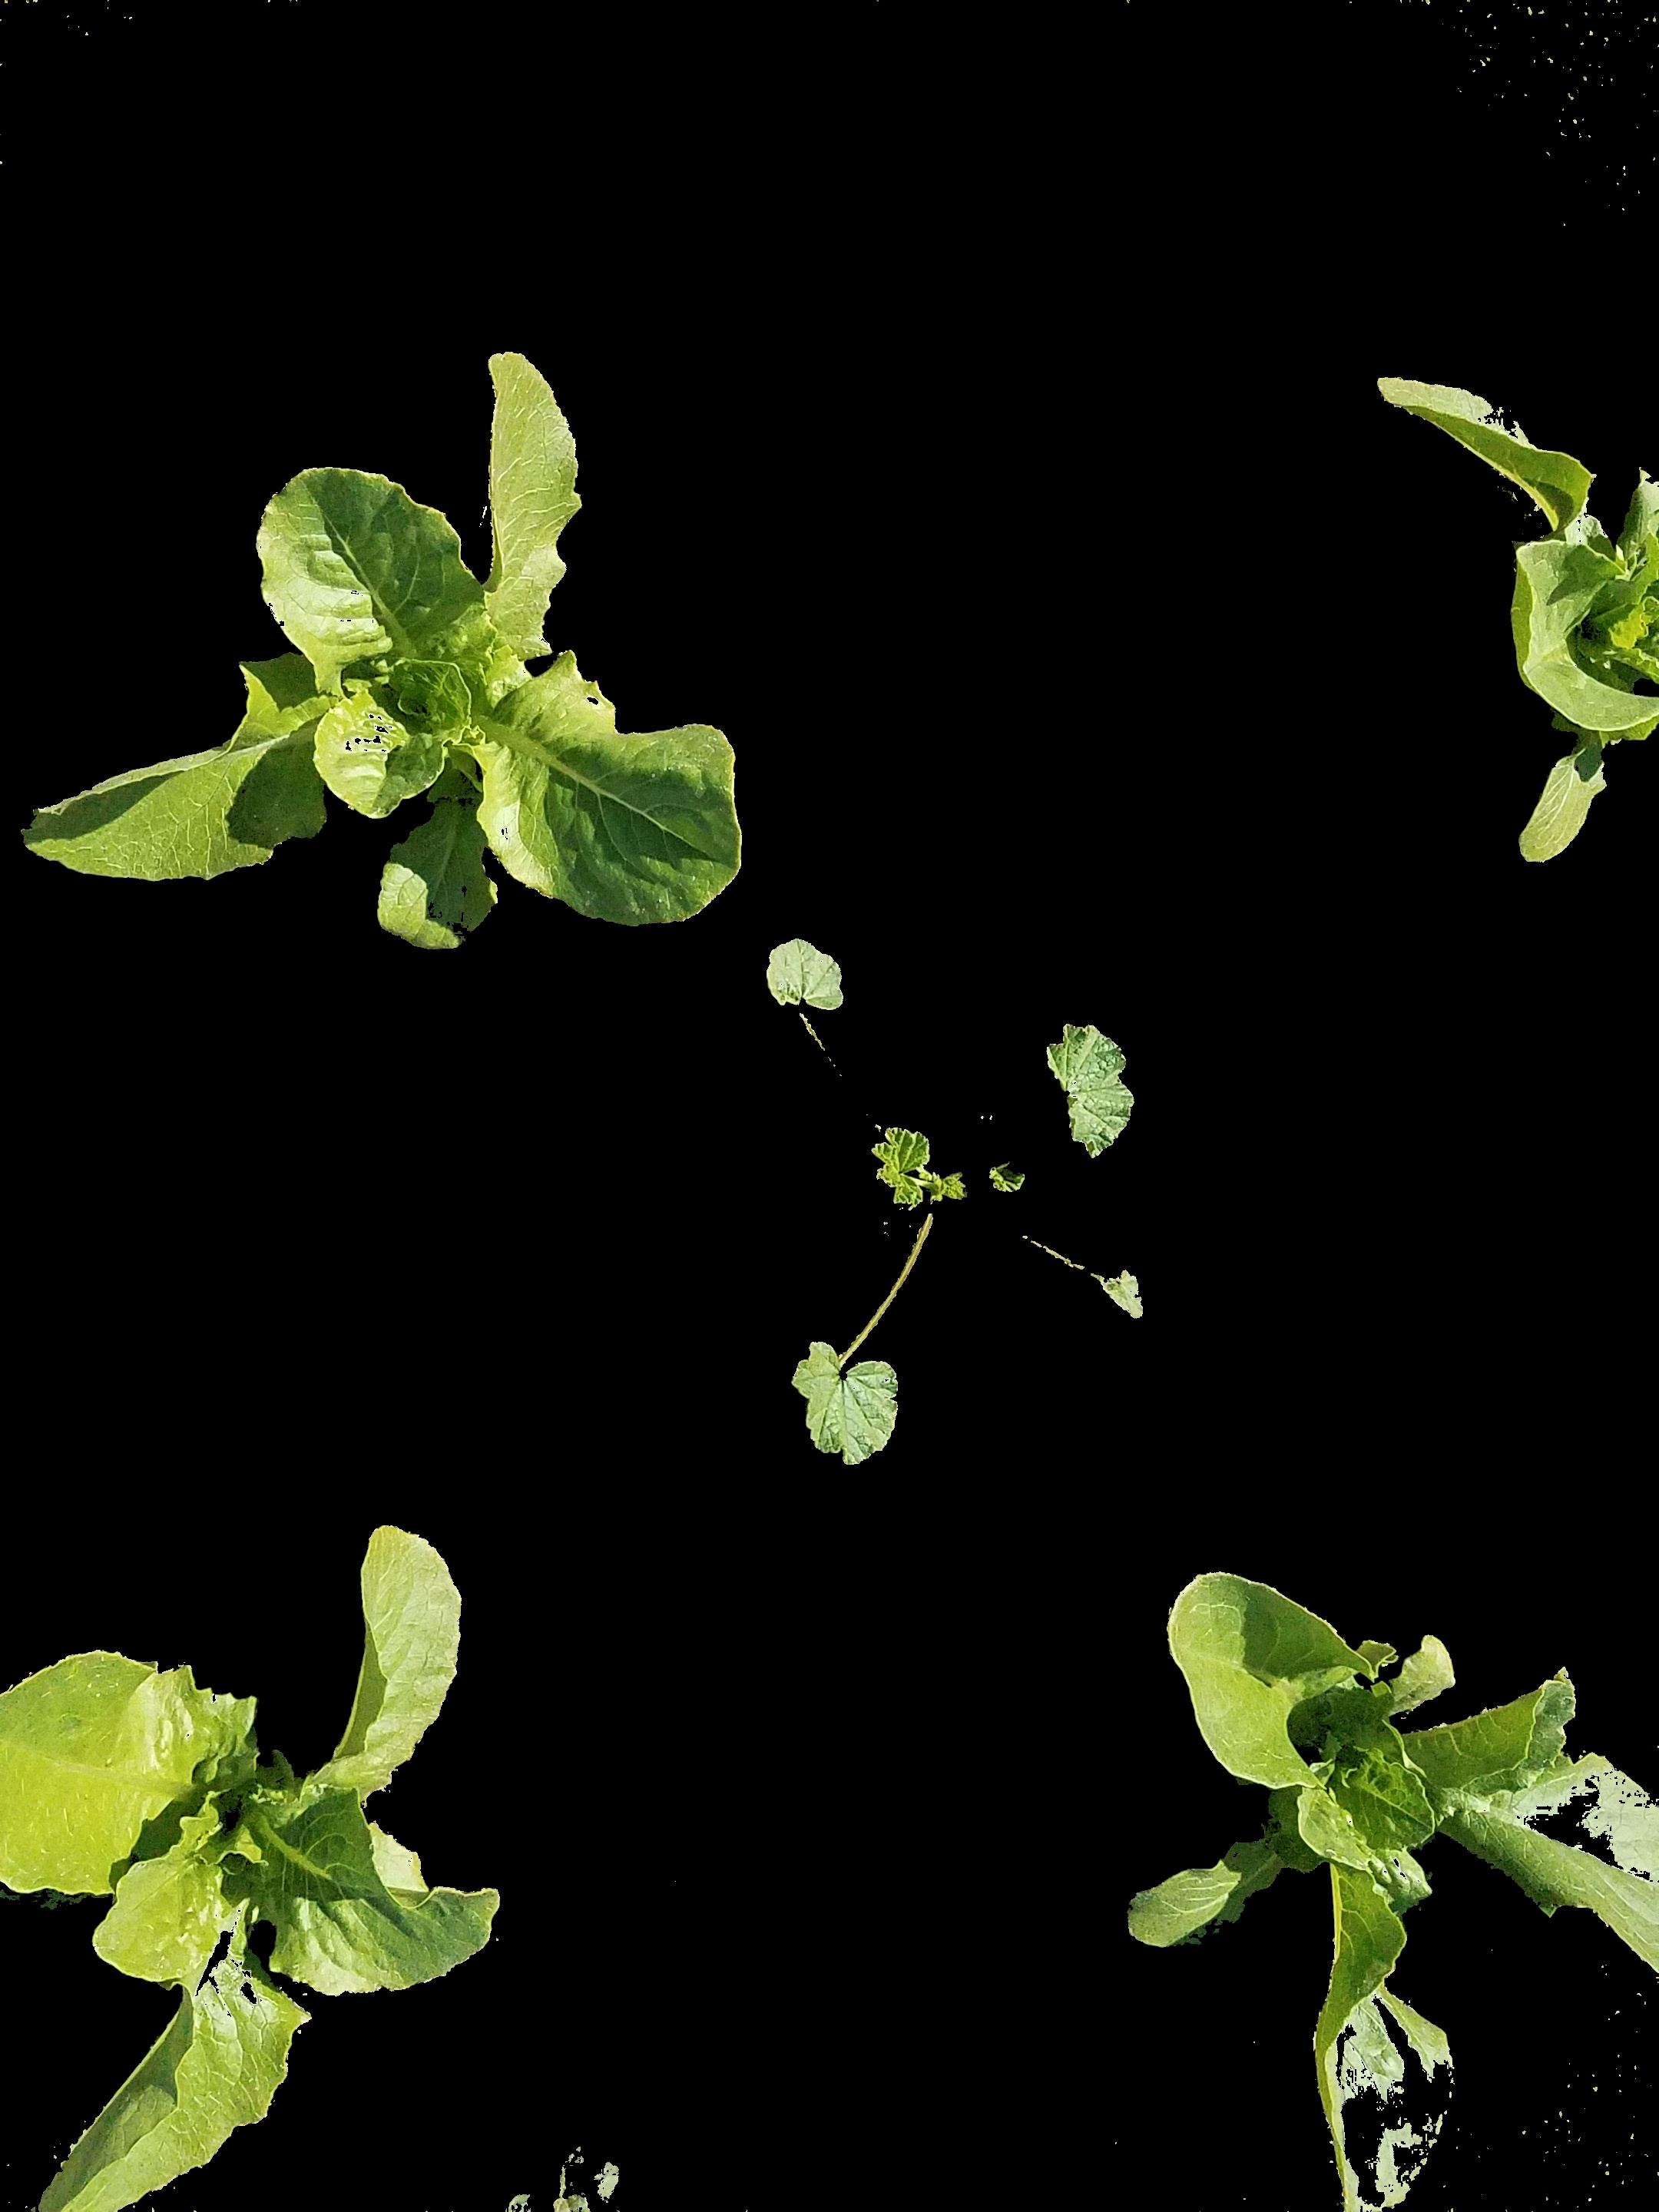
\includegraphics[height=0.10\textheight]{figures/20201117_112624-COM2.jpg} \label{fig:com2}}&
\subfloat[MEXG]{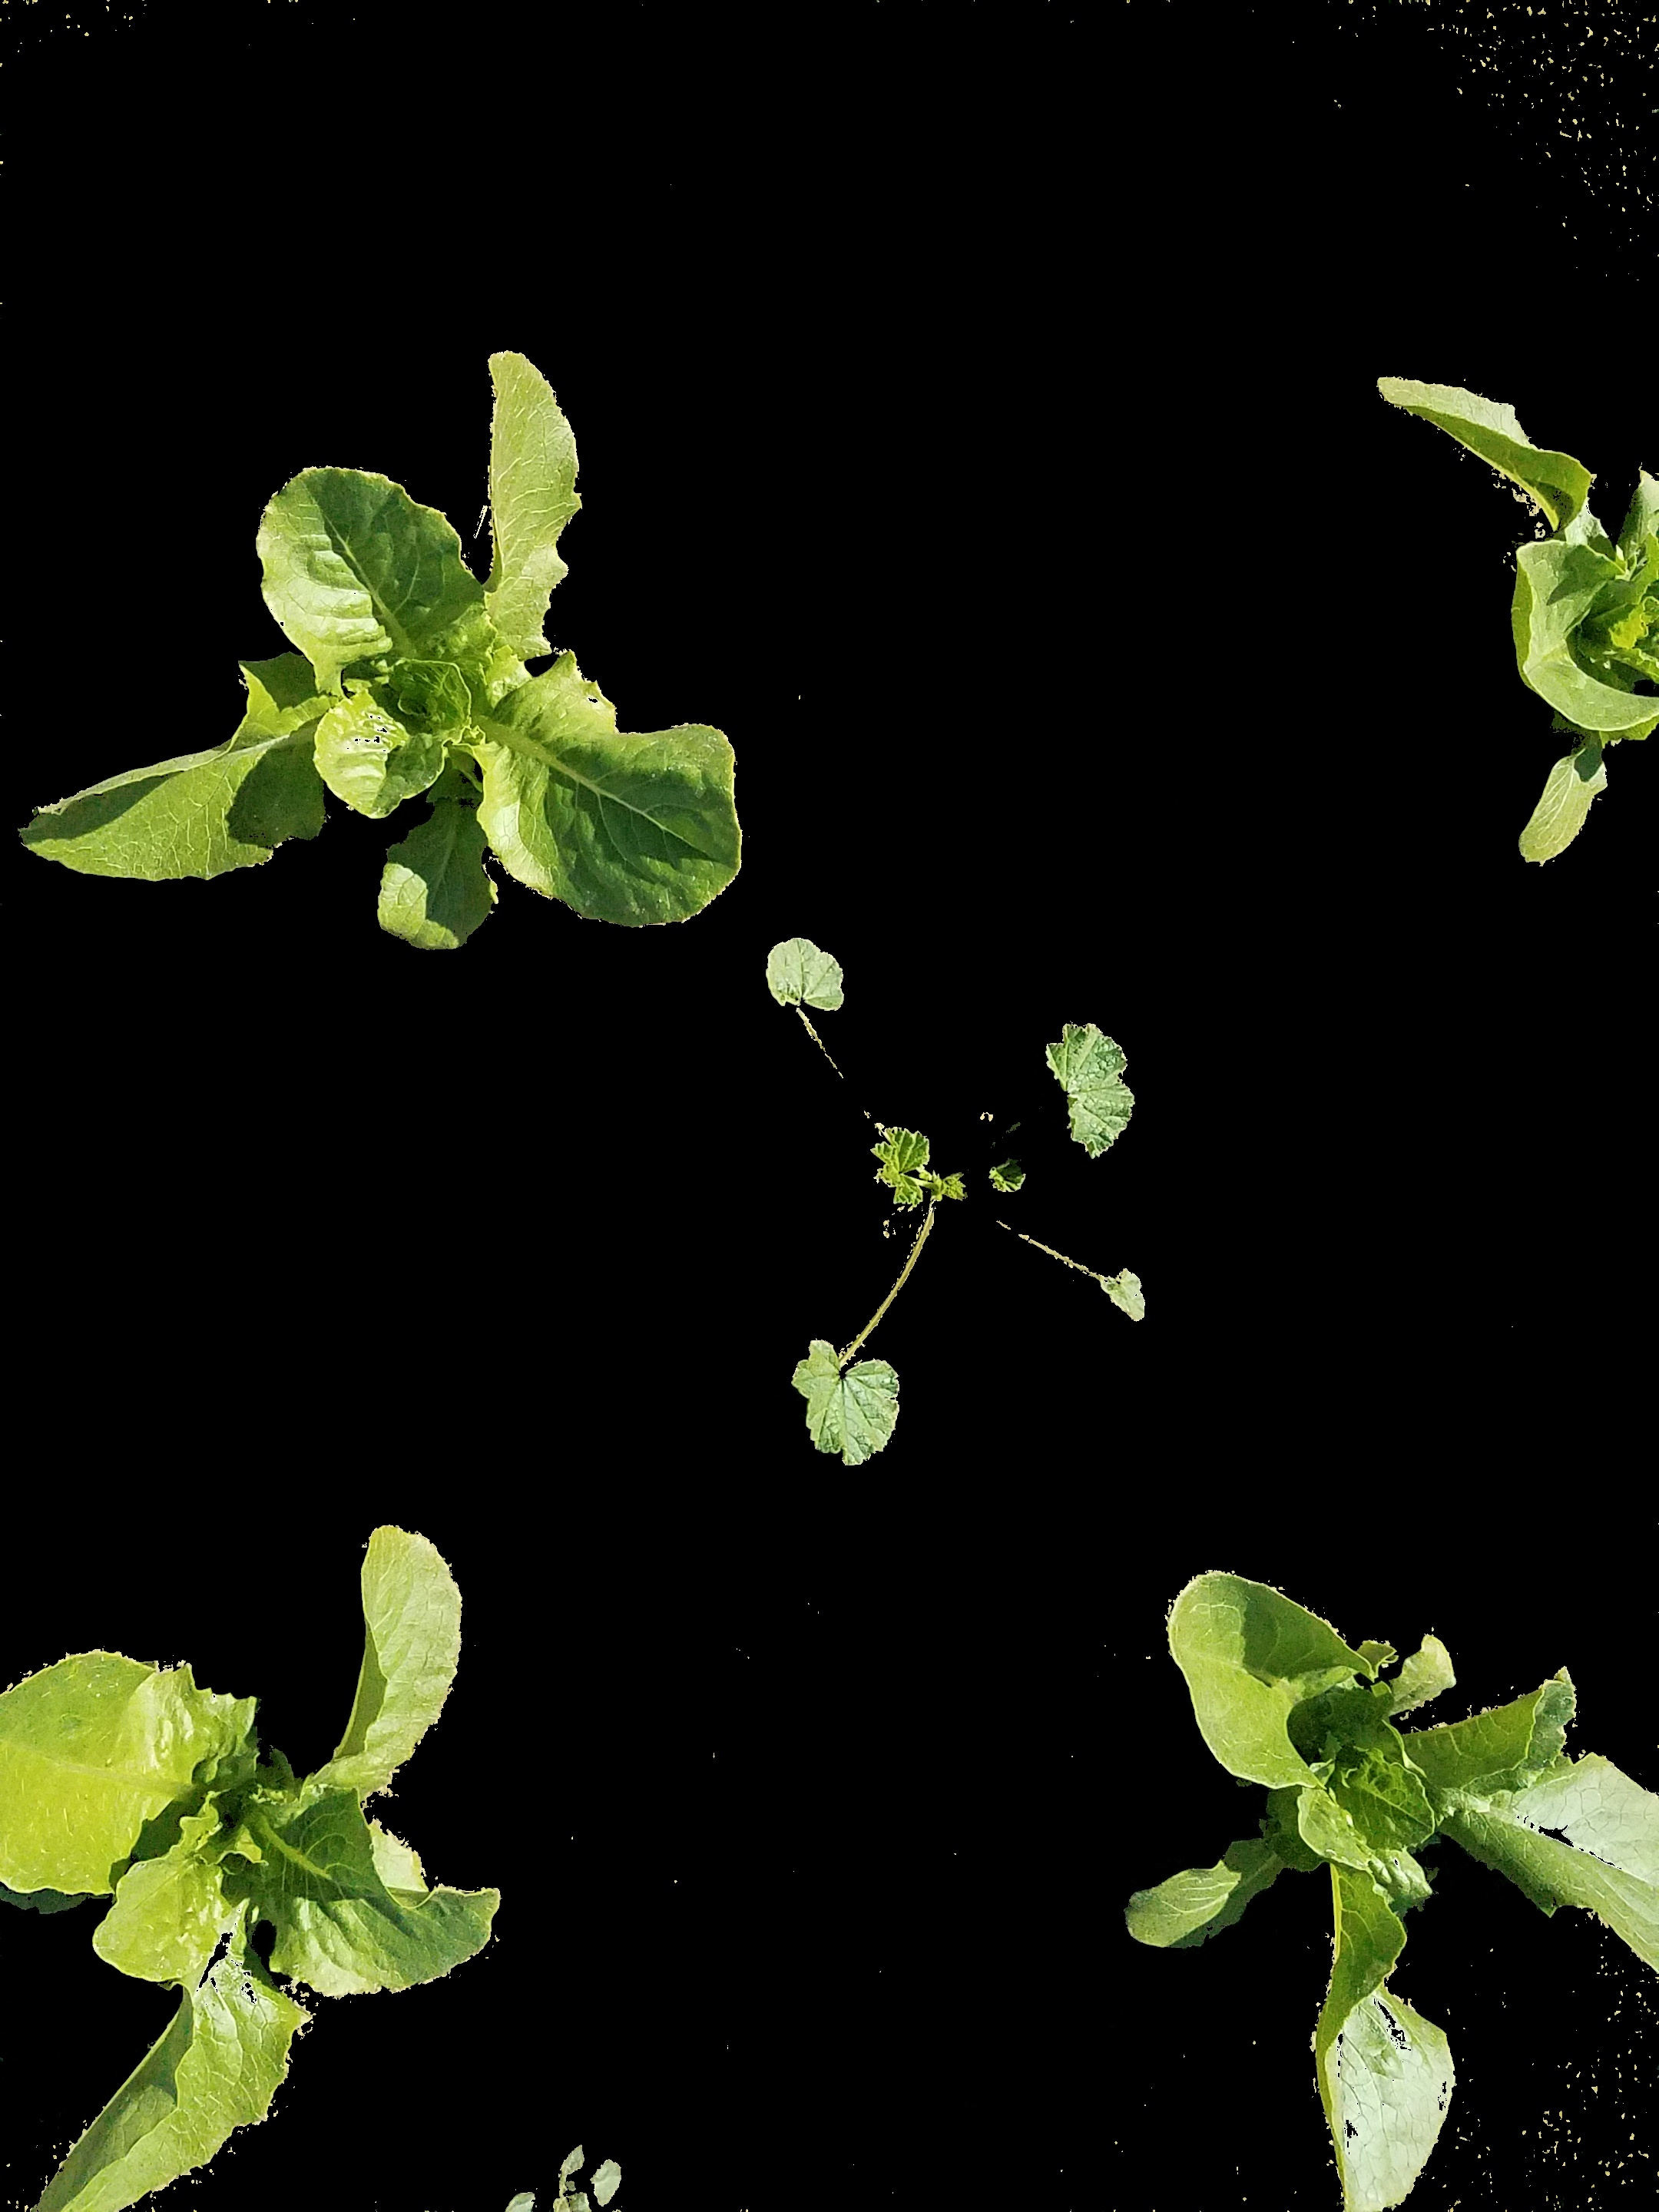
\includegraphics[height=0.10\textheight]{figures/20201117_112624-MexG.jpg} \label{fig:mexg}} &
\subfloat[TGI]{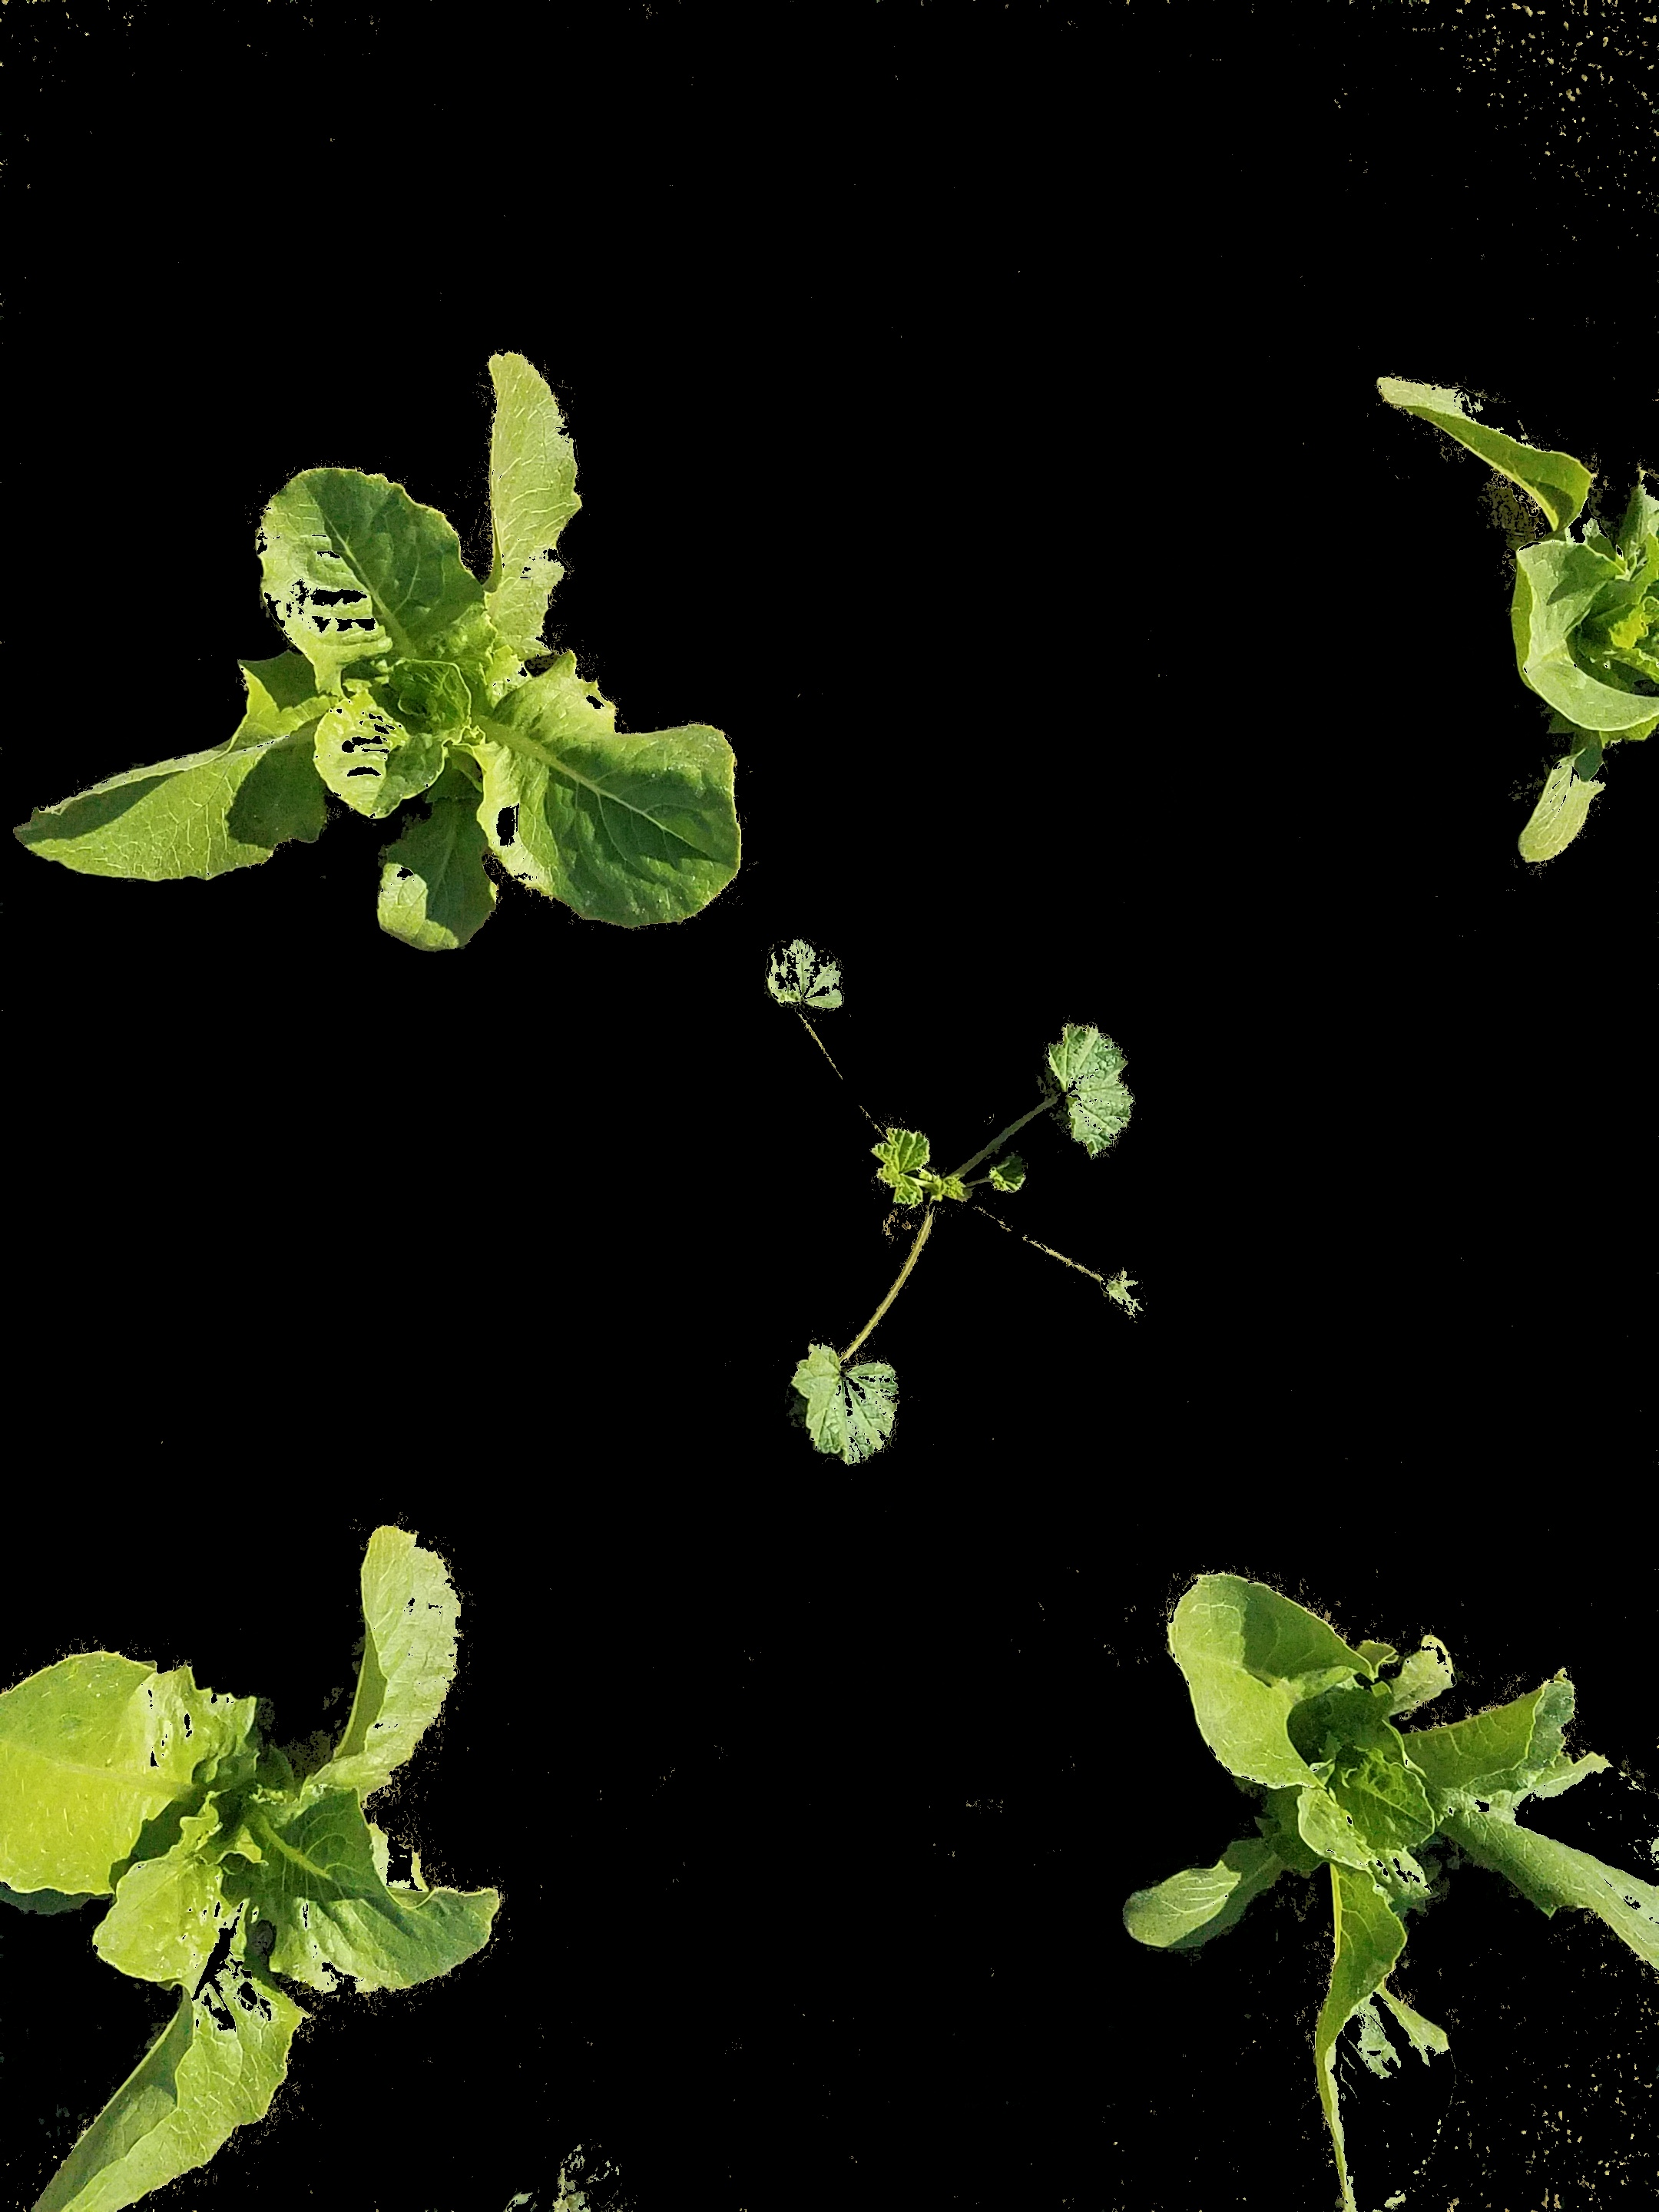
\includegraphics[height=0.10\textheight]{figures/20201117_112624-TGI.jpg} \label{fig:tgi}} &
\subfloat[VEG]{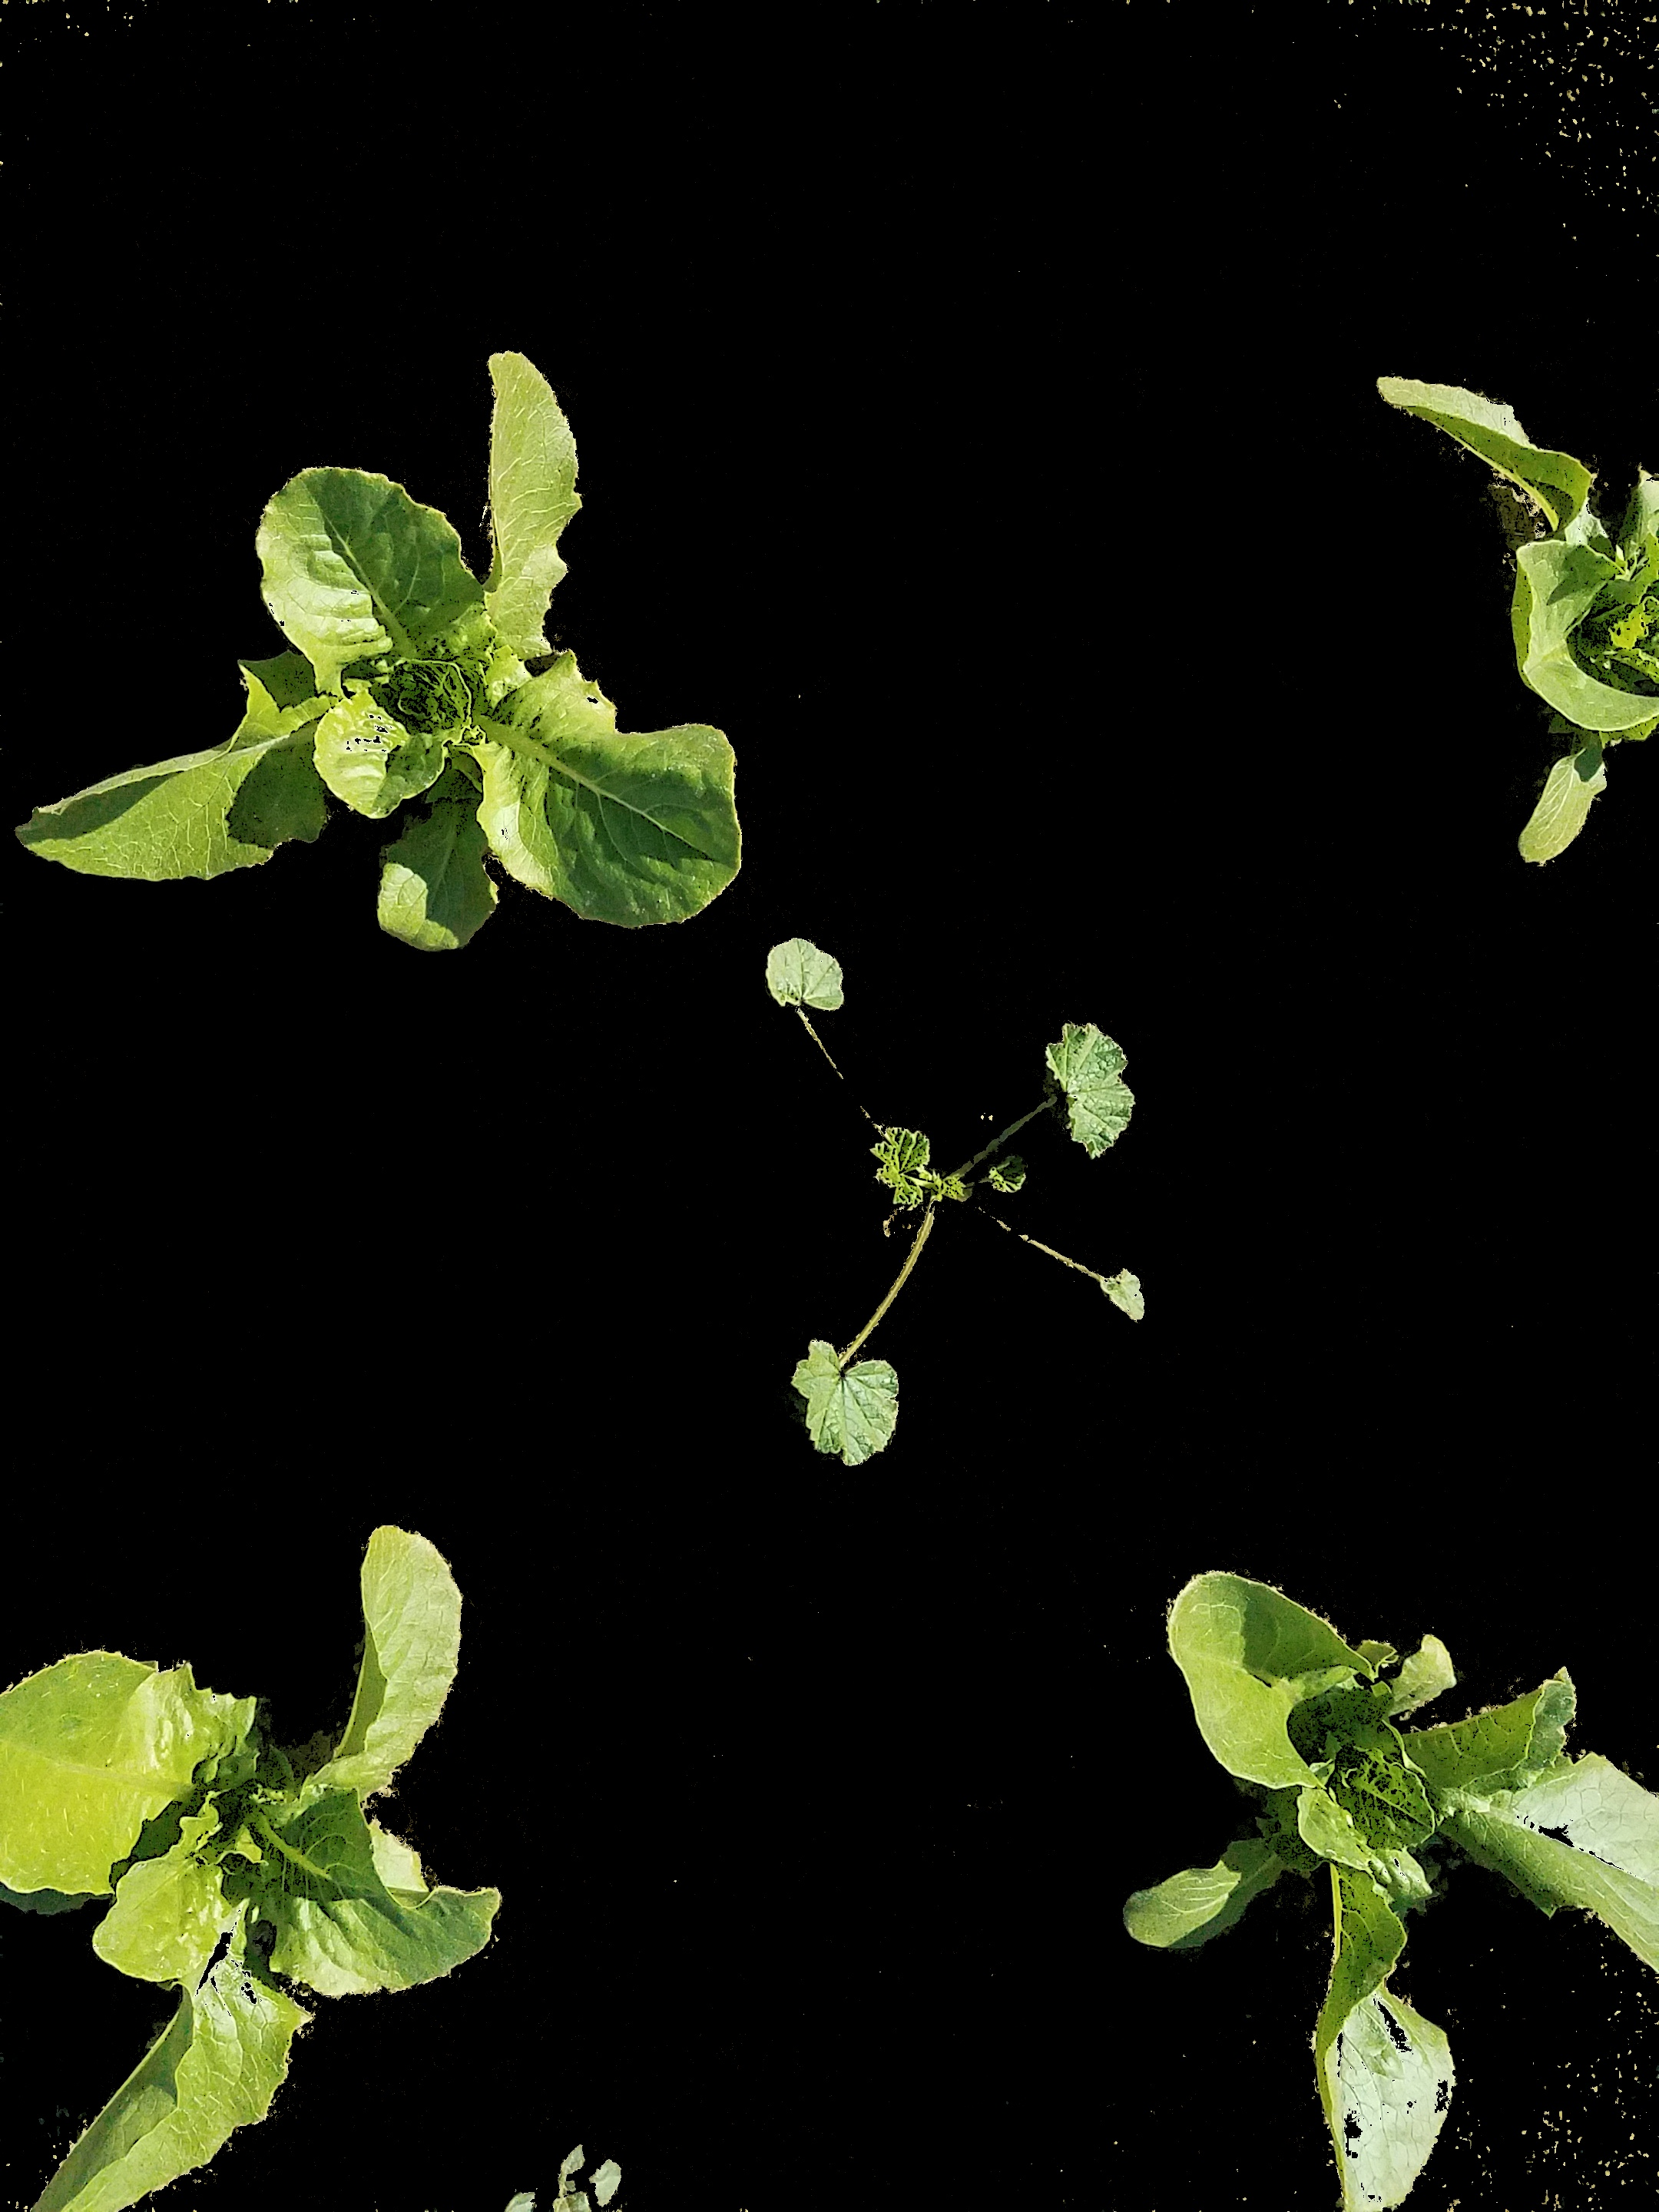
\includegraphics[height=0.10\textheight]{figures/20201117_112624-VEG.jpg} \label{fig:veg}} &
\subfloat[Original]{\includegraphics[scale=0.0215,angle=90]{figures/20201117_112624.jpg} \label{fig:original}} \\

\end{tabular}
\caption[Results of various visible-light image segmentation techniques]{Various visible-light image segmentation techniques (See Table \ref{table:indices} for details) with the index threshold chosen using the Triangle algorithm. At first glance, many of the segmentation algorithms produce similar results, but some of the methods are not sensitive to less green portions of the plants -- slender stems. Contrast the results seen in \ref{fig:exr} and \ref{fig:mexg}, with the slender stems of the plant in the middle of the image not present in the result of the former.}
\label{figure:results}
\end{figure}

There are two potential mistakes encountered during segmentation, as there are only two classes in the image: pixels that are vegetation (crop and weeds) and pixels that aren't (typically, the ground, but also items that are expected to appear, such as irrigation equipment). Omission of a crop leaf is apparent in Figure \ref{fig:ndi}, showing the result of using NDI.  The center plant is only partially visible in this case, and what is not retained cannot be classified. Contrast that with the result shown in Figures \ref{fig:hi} and  \ref{fig:hv}, where the ground is featured. This case may be due to the shadow of the plant containing too much green as sunlight passes through the leaf. Figure \ref{fig:overlay} illustrates the effects of the index and errors -- of special note here is the error that is shown in the upper right-hand portion of Figure \ref{fig:overlay-cive}. These errors may result in the ground mistakenly identified as vegetation. Applying the NDI mask produces the errors discussed previously -- the leaf shadow is identified as vegetation. The evaluation of errors in index-based approaches is illustrated by Figure \ref{fig:segmentation-errors}.

\begin{figure}[H]
	\centering
	\subfloat[CIVE mask overlay\centering]{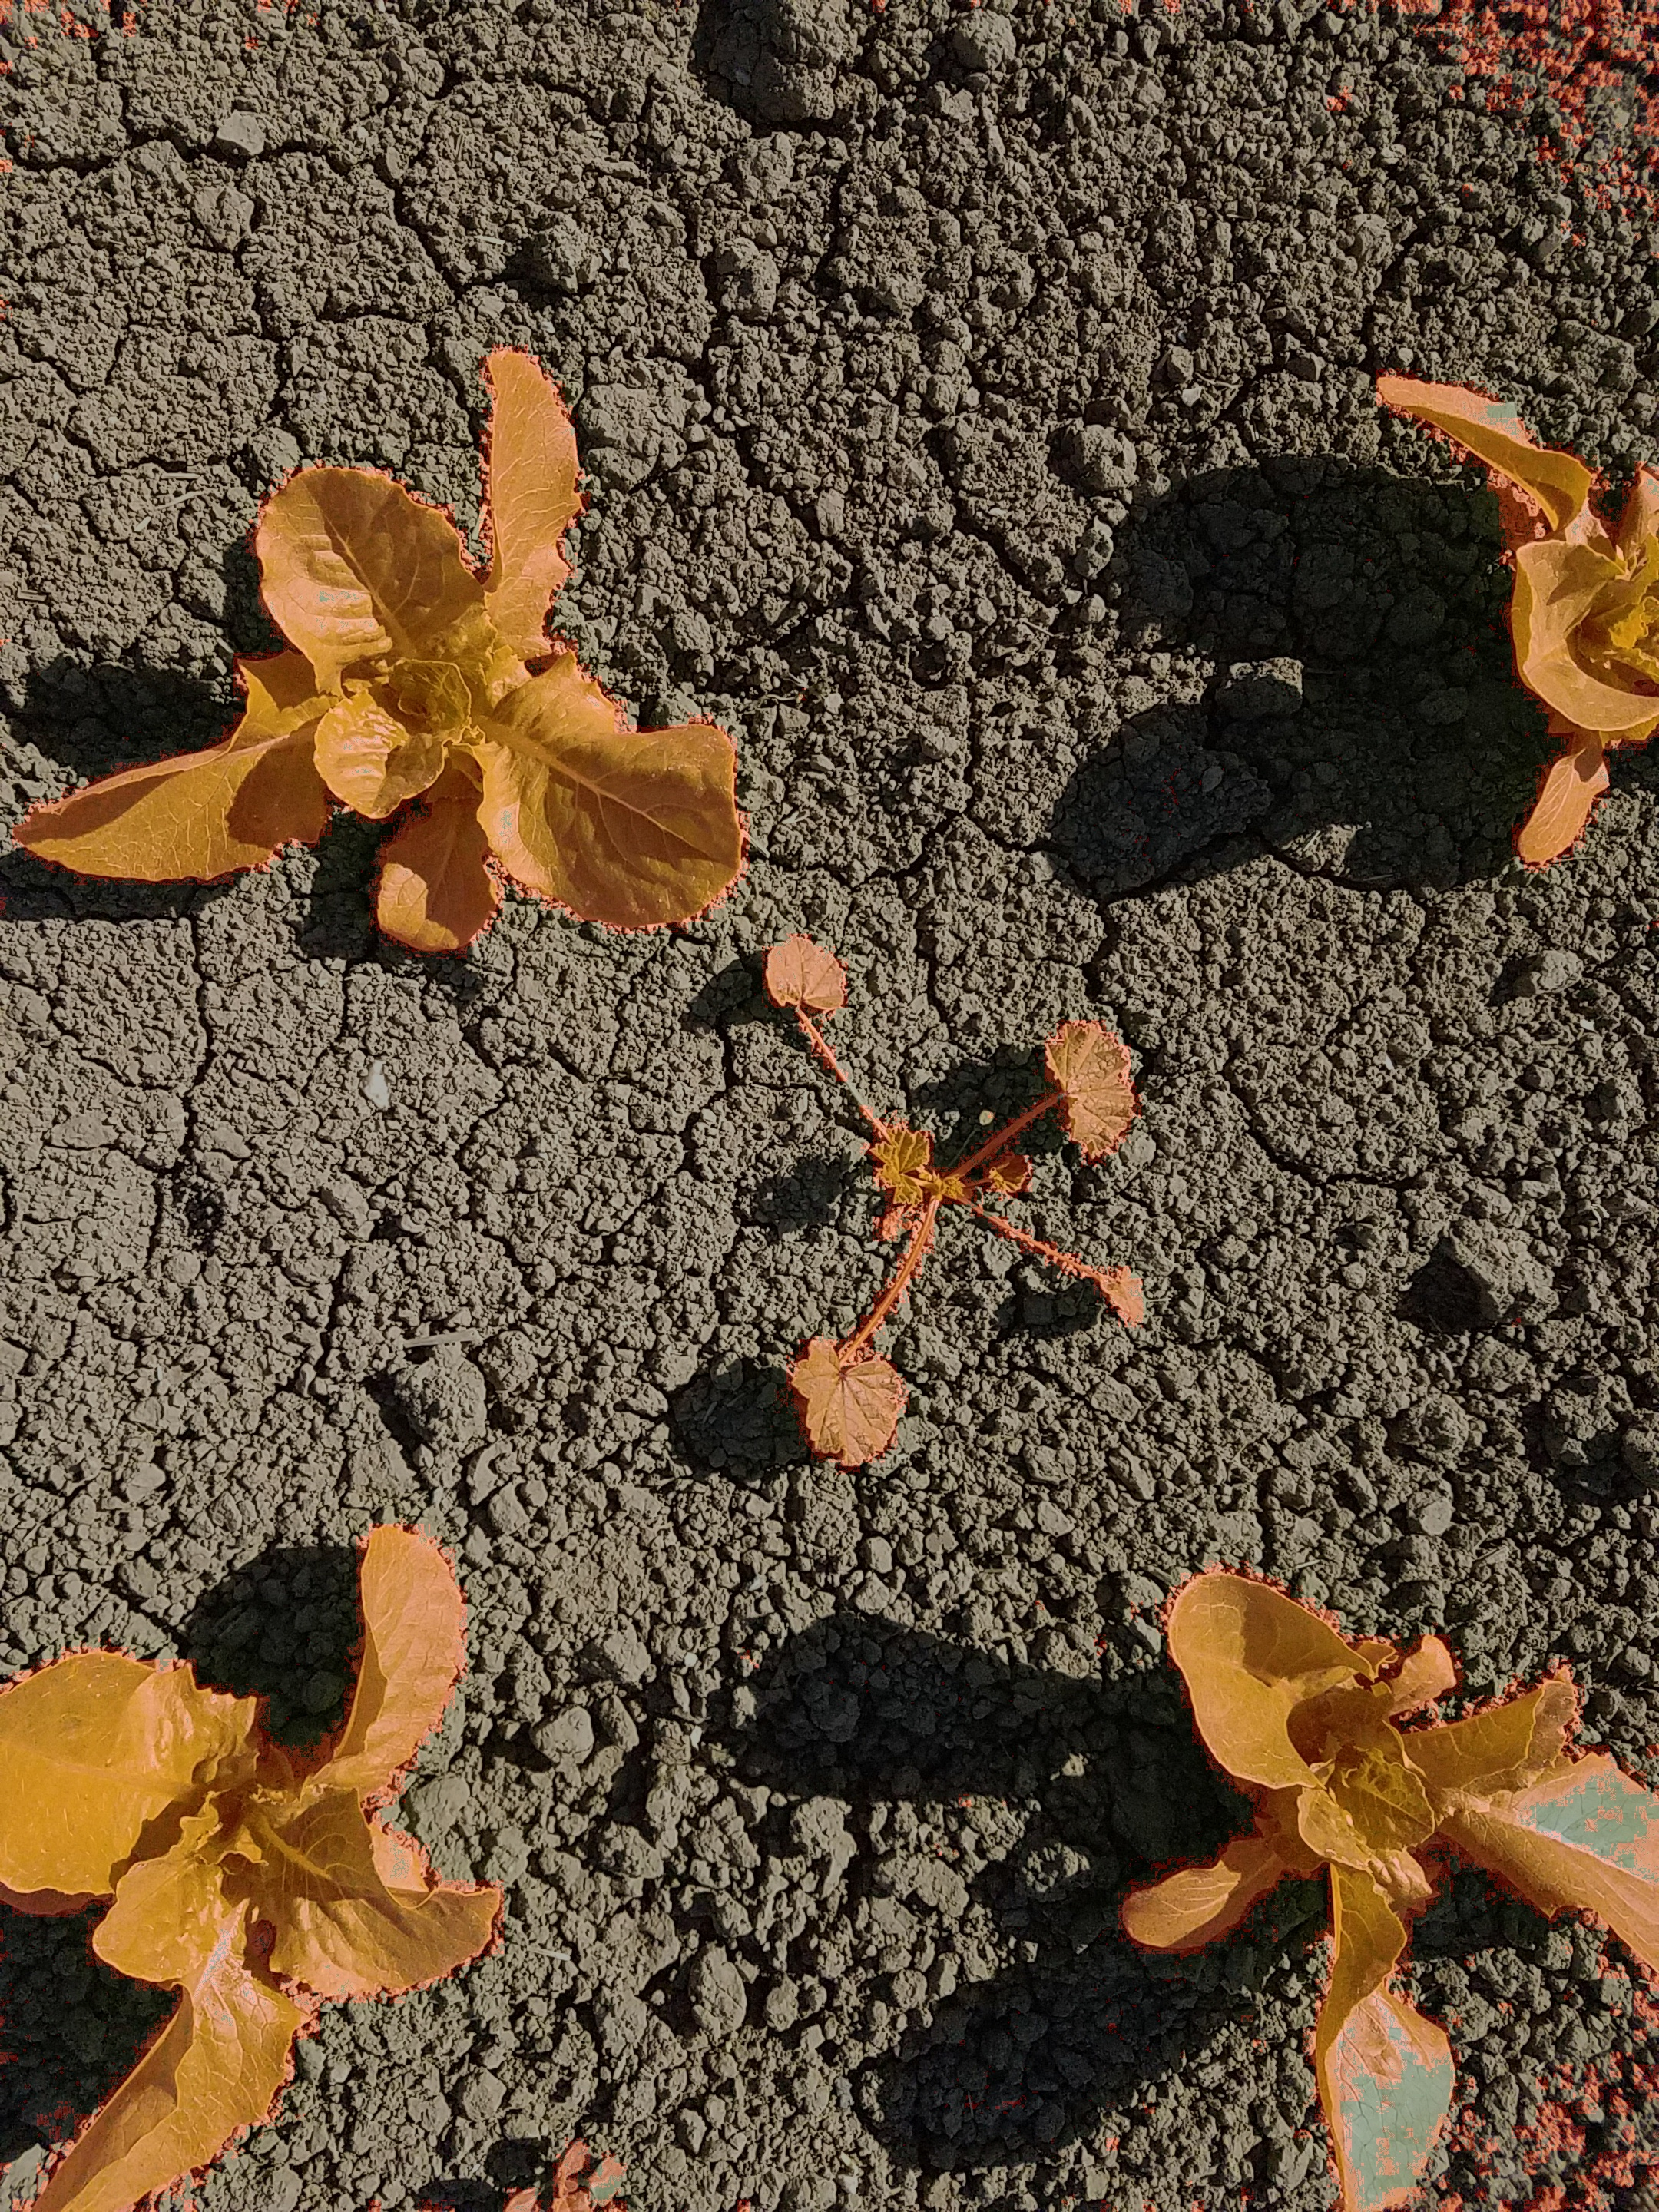
\includegraphics[width=0.45\textwidth]{figures/overlay-cive.jpg}\label{fig:overlay-cive}}
	\hfill
	\subfloat[NDI mask overlay\centering]{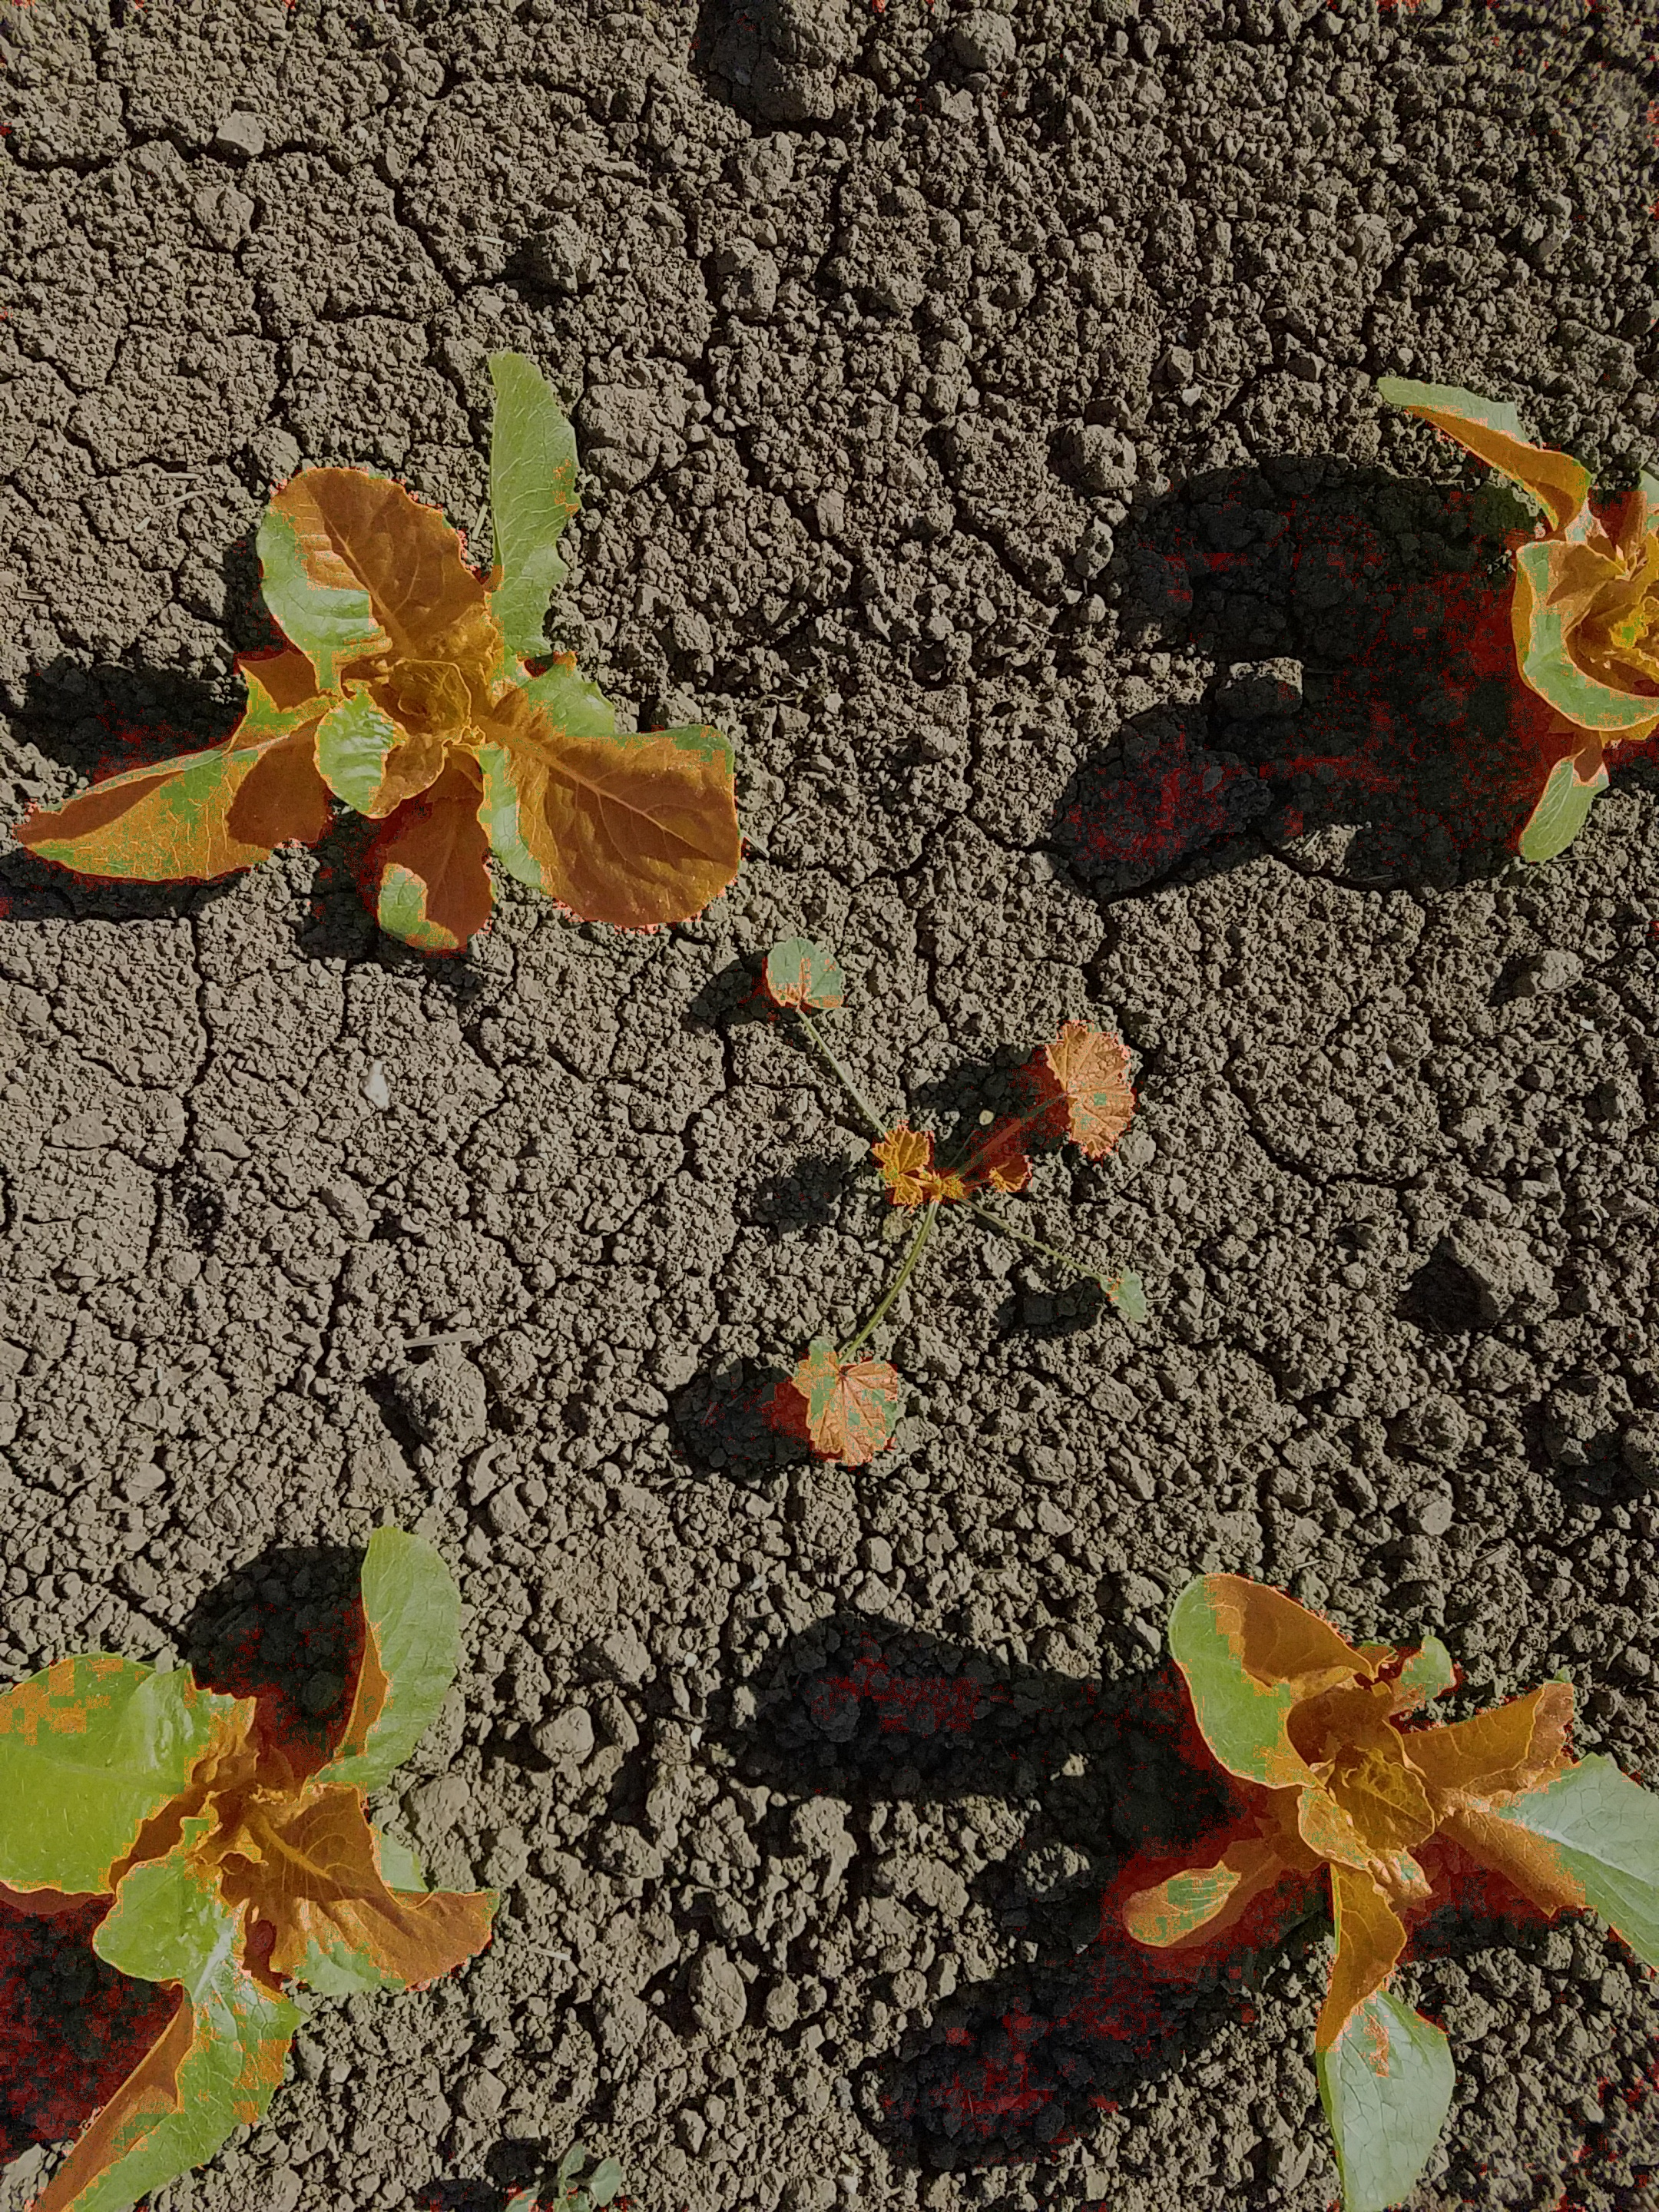
\includegraphics[width=0.45\textwidth]{figures/overlay-ndi.jpg}\label{fig:overlay-ndi}}
	\caption[Masks overlayed on original images]{Masks produced with CIVE and NDI overlayed on the original image. In these images, the masks used are colored red and blended with the original image. Areas that are tinted red will be shown, so a `correct' mask will completely cover vegetation. Note the mask shown in \ref{fig:overlay-ndi} does not cover the plant completely, and segments out shadow portions of the image. This may have resulted from sunlight shining through the leaf, making the ground green enough to be interpreted as vegetation. In c contrasting with 9a, where portions of the ground are incorrectly segmented as vegetation not due to color contamination. (The upper right-hand portion of \ref{fig:overlay-cive} is a good example of this error.) Photo: Dr. Mark Siemens, University of Arizona.}
	\label{fig:overlay}
\end{figure}

\subsection{Alternative Color Spaces}
While the RGB color space is ubiquitous and intuitive, relying solely on it for image segmentation in complex real-world environments—such as agricultural fields—can present limitations. These limitations arise primarily due to the inherent variability in lighting conditions, soil background interference, and subtle color distinctions between objects of interest, such as crops and weeds. To address these issues, index-based segmentation techniques have expanded into alternative color spaces beyond RGB, notably Hue-Saturation-Intensity (HSI), Hue-Saturation-Value (HSV), YCbCr, YIQ, and CIELab, which may offer improved segmentation accuracy under varying environmental conditions.

RGB indices, such as Excess Green (ExG) or Normalized Difference Vegetation Index (NDVI), are effective at distinguishing green vegetation from soil backgrounds. However, these indices typically assume that vegetation is uniformly green, which is often not true in field conditions. Plants exhibiting non-green features—such as red stems in Purslane (Portulaca oleracea) or purple leaves in red-leaf lettuce—often result in segmentation errors because RGB-centric indices tend to exclude these areas, considering them as background.

Additionally, RGB indices may not reliably discriminate between vegetation and soil, particularly under varying illumination conditions, leading to either false positives (soil pixels identified as vegetation) or false negatives (vegetation identified as soil). Thus, to improve segmentation accuracy, alternative color spaces that decouple brightness and chromaticity have become increasingly valuable.

Nevertheless, segmentation using alternative color spaces presents certain challenges. Determining optimal thresholds in non-RGB spaces can be more complex than in RGB, as each channel represents different information. Additionally, computational complexity slightly increases as RGB images must first be transformed into alternative spaces before segmentation can occur. However, these added complexities are typically outweighed by the increased segmentation accuracy and reliability.

\subsubsection{HSI and HSV}
The Hue, Saturation and Intensity (HSI) and Hue Saturation and Value (HSV) color spaces present an opportunity to consider how saturated the colors are instead of just emphasizing the green found it an image. While that is  an over-simplification of basing a technique on the values found within the RGB bands, it is essentially what is happening. Hue based approaches take much the same approach in one respect -- the hue frequently present in vegetation (green) is represented as peaking around $120^o$ in both models. This is convenient, certainly, as simply considering points as vegetation of they contain hue values around the peak. How wide this range is, of course, will determine what is captured. And while the topic of color is revisited in Section ~\ref{section:problems-color}, consider that leaves contain much that is not green, just as the ground contains much that is not brown. A leaf may contain hue values in the range of 40-70, an indication that the hue is toward the red end of the representation. Likewise, a patch of dirt may contain hue values in the range of 15-20, an indication that the hue is much more red than anything else. HSV is  more complicated, in that the V band should be normalized between $(0..1)$ and multiplied by the H value. These indices will be referred to as HI and HV. 

\begin{equation}
	\label{equation:hsi}
	HSI
    \begin{split}
		discard~pixels~with~H~channel &\geq 190~or \leq 55\\
		discard~pixels~with~S~channel &\leq 0.45 \\
		discard~pixels~with~I~band &\geq 50
    \end{split}
\end{equation}

\begin{equation}
	\label{equation:hsv}
	HSV
	\begin{split}
		H * norm(V) \\
	\end{split}
\end{equation}

\subsubsection{CIELAB}
The CIELAB color space, often referred to with L*A*B* in the name, expresses color along three lines: Lightness (L), Green-Red (A), and Blue-Yellow (B). These values seen in these bands have different ranges, L ranging from 0 (black) to 100 (white), A ranging from negative (green) to positive (red), and B ranging from negative (blue) to positive (yellow). The A and B bands are not technically limited to a specific range, as this space was designed to exceed human perception. Human perception of these colors can be covered with a $\pm 150$ range, and implementations tend to limit the values reported in these bands for practical reasons.  For the purposes of indexing vegetation the bands of  most interest are the A and B bands. Taking the difference between B and A and discarding pixels with a difference is below 30 yields acceptable results. This index will be referred to as CI throughout this document.

\begin{equation}
		\label{equation:cielab}
		B - A, discard~results~\leq~30
\end{equation}

\subsubsection{YCbCr}
This color space (sometimes termed YCC) is frequently encountered in video transmission, as it is designed to address the redundancies seen in the RGB color space. It uses the $Y$ channel to carry Luma information (black and white) and two color channels expressing the blue difference (Cb) and red difference (Cr). Separating the brightness from the color components allows the color representations to match human perception -- as our eyes are more sensitive to changes in brightness than they are to color. As with other indices, the objective is to exaggerate the band vegetation occupies and ignoring components that are not. Using equation \ref{equation:ycbcr} achieves that goal.
\begin{equation}
	\label{equation:ycbcr}
	\ln(Cr) * Cb, discard\ results\geq 890
\end{equation}
This index will be referred to as YCbCRI throughout this work.

\subsubsection{YIQ}
The YIQ model of color was used by the  National Television System Committee (NTSC) analog color TV system. Later, digital transmission schemes used different color spaces, notably the YCbCr that will be addressed in more detail in a separate section. These schemes have a common approach: \textit{chrominance} (a color component) is added to a black and white image. In the YIQ model, $Y$ represents the luminance information (black and white), with $I$ (in-phase, representing red-cyan contrast) and $Q$ (quadrature, representing magenta-green contrast) the chrominance information. 
The processing employed here is to convert the image to the YIQ color space and take the mean value for the $I$, or in-phase component for the blob's pixels. (\cite{MathWorks_undated-jg}) For segmentation purposes, the information in the Q band is helpful, primarily in discarding things that are not vegetation.
\begin{equation}
	\label{equation:yiq}
	discard\ any\ pixel\ with\ Q\ band\leq 0.04
\end{equation}
This index will be referred to as YI throughout this document.

\begin{figure}[H]
\centering
\begin{tabular}{ccc}
	\subfloat[CIElab]{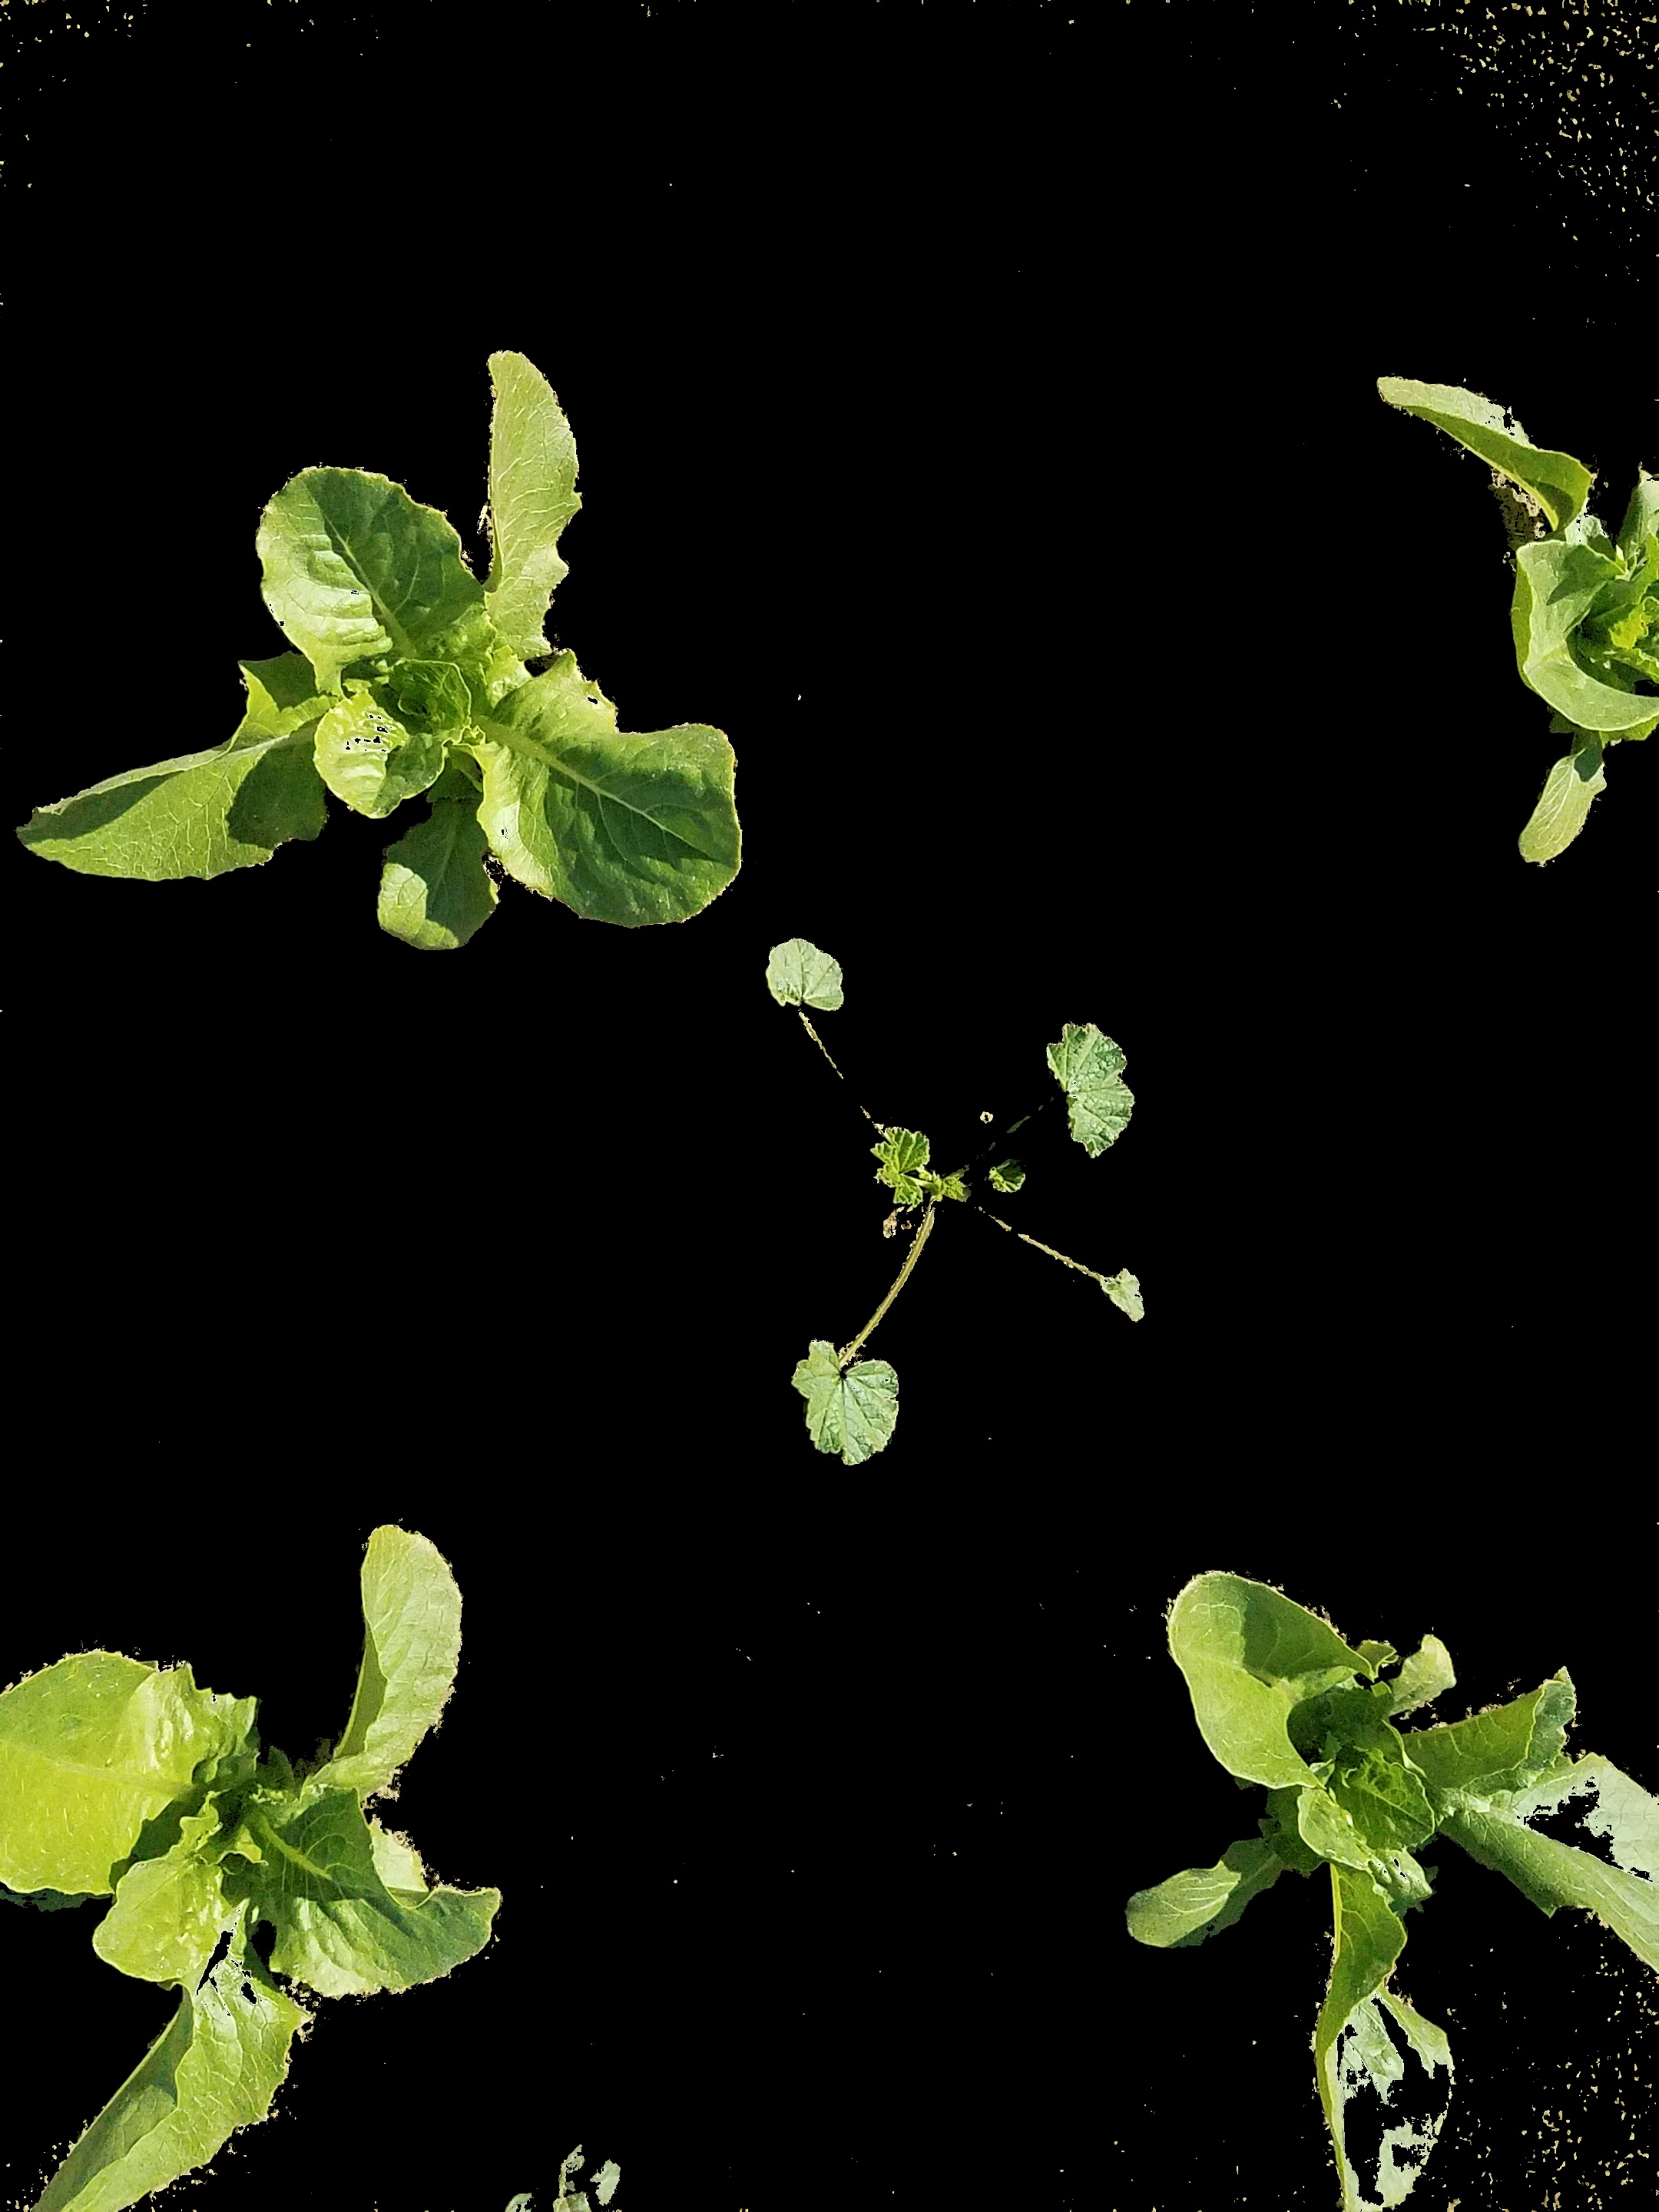
\includegraphics[width = 1.25in]{figures/20201117_112624-CI.jpg} \label{fig:ci}} &
	\subfloat[HSI]{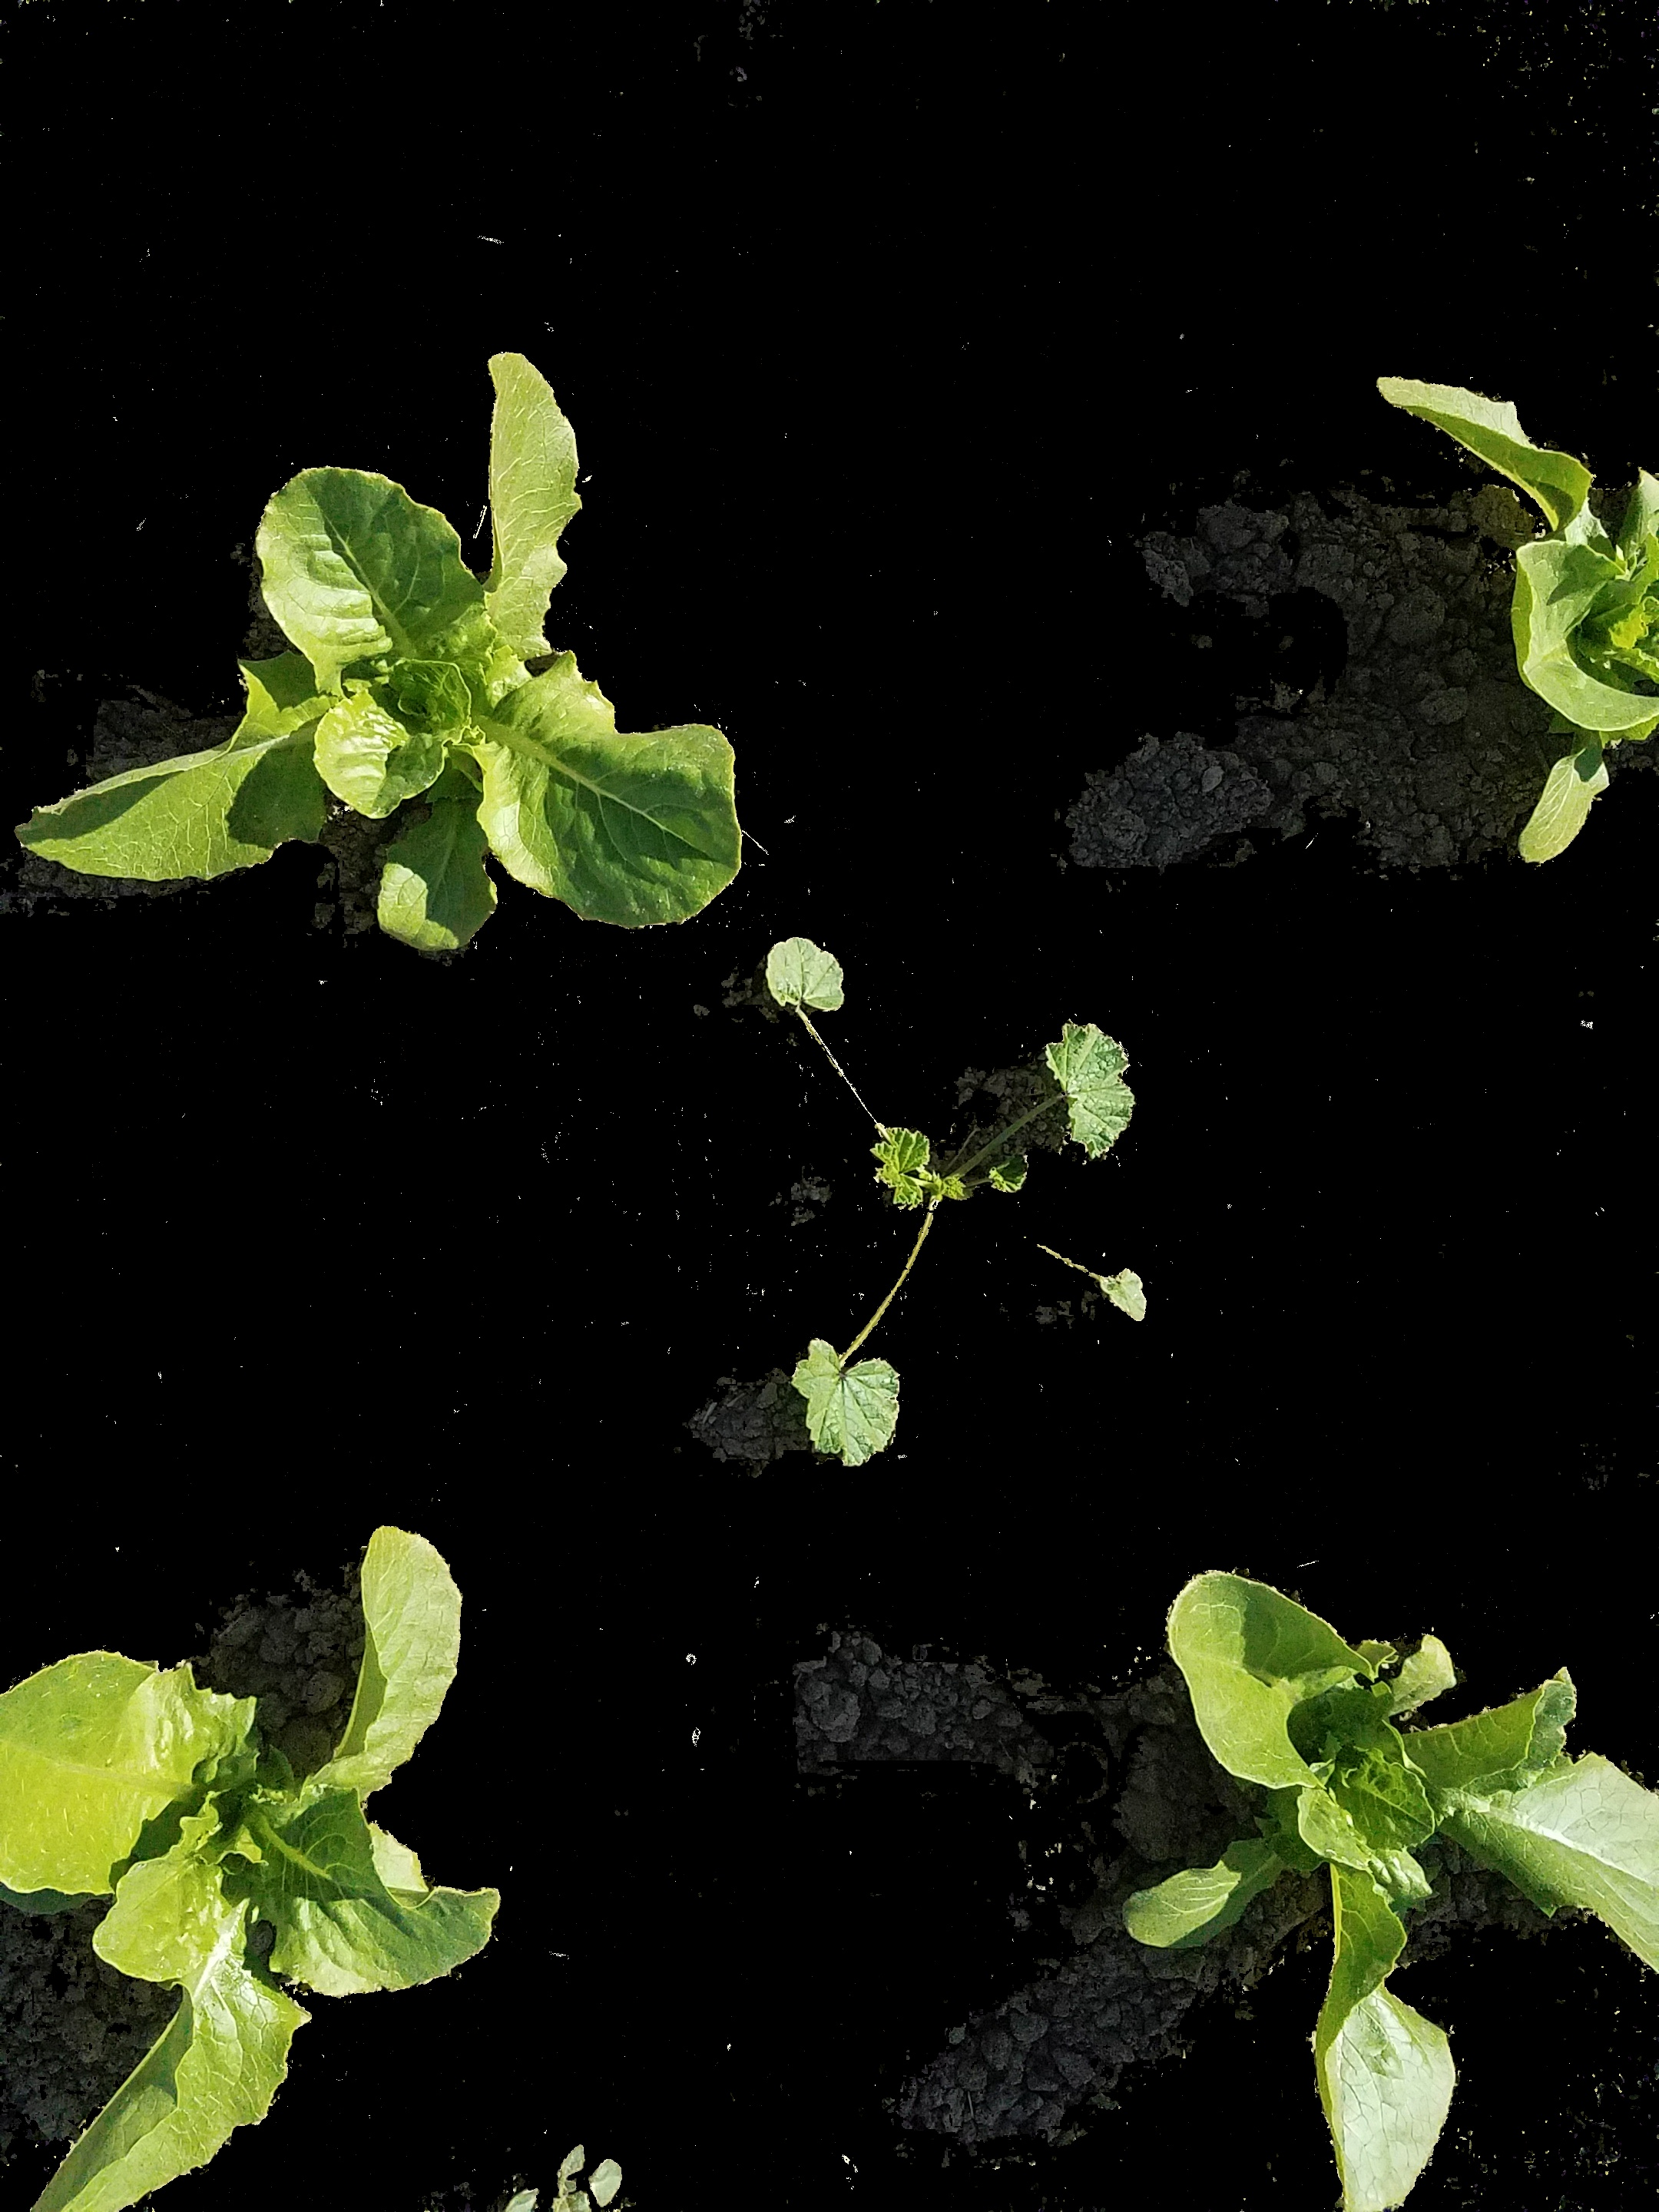
\includegraphics[width = 1.25in]{figures/20201117_112624-HI.jpg} \label{fig:hi}} &
	\subfloat[HSV]{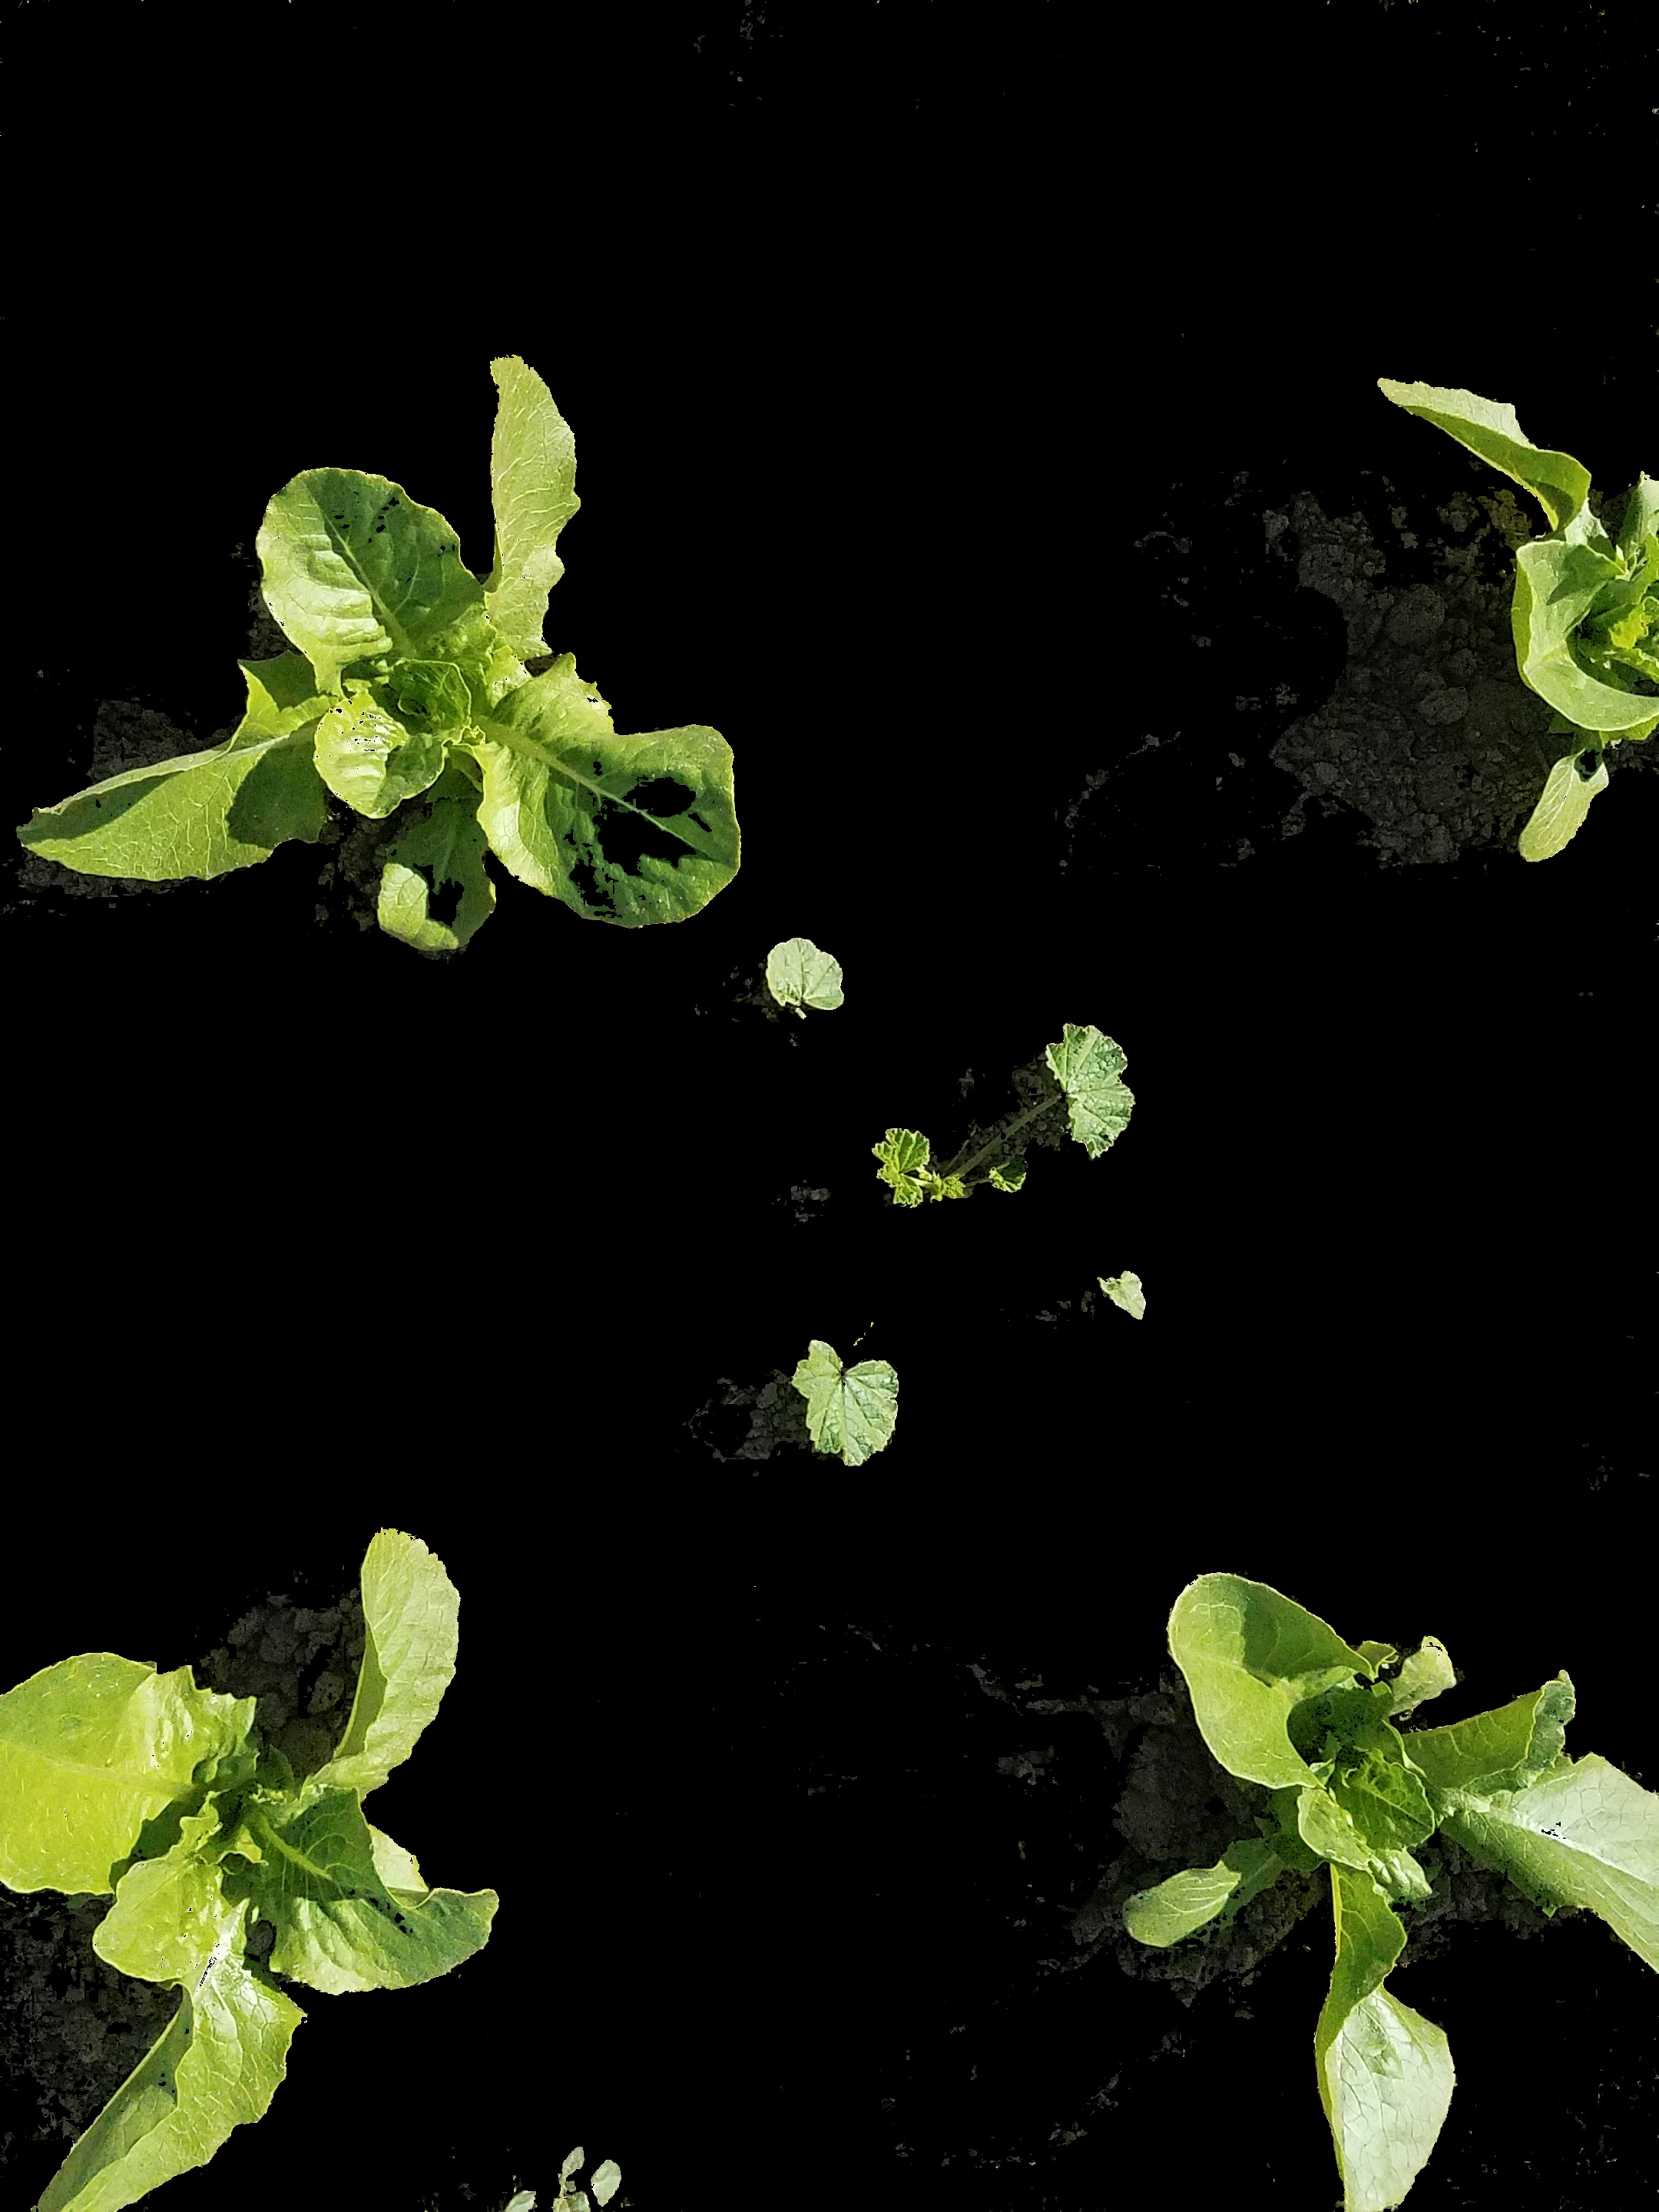
\includegraphics[width = 1.25in]{figures/20201117_112624-HV.jpg} \label{fig:hv}} \\
	\subfloat[YCbCr]{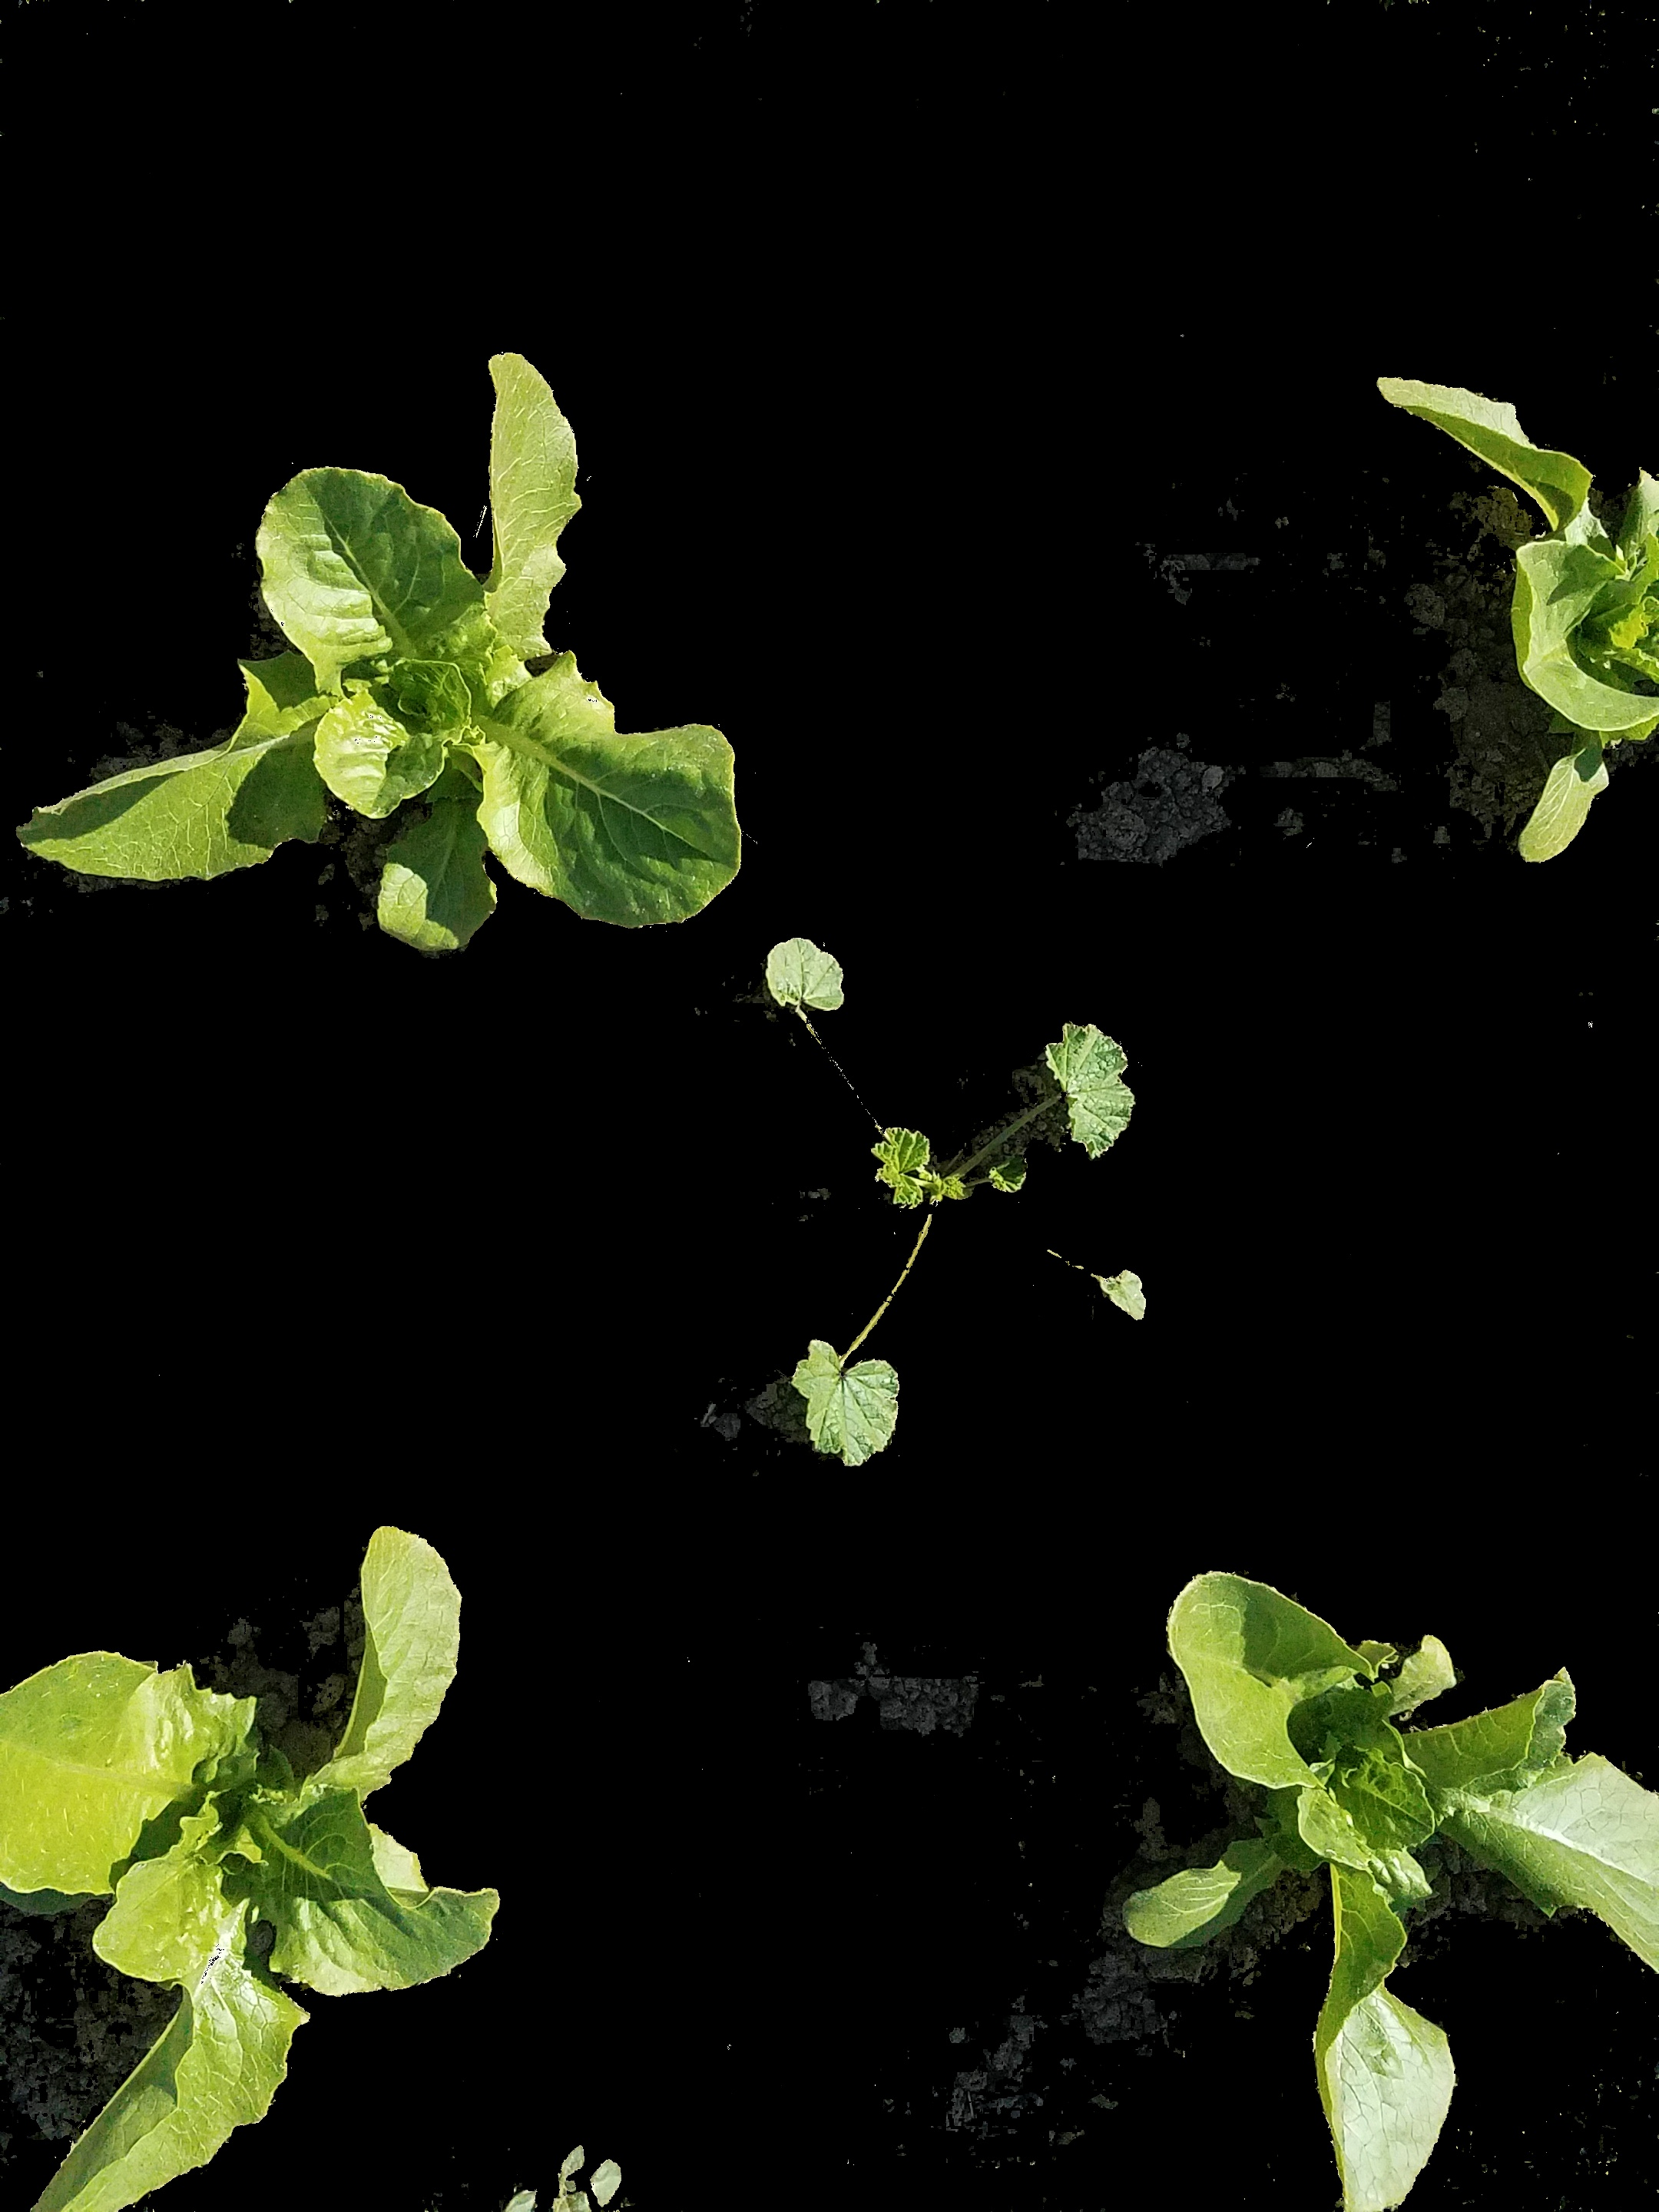
\includegraphics[width = 1.25in]{figures/20201117_112624-YCbCrI.jpg} \label{fig:ycbcr}} &
	\subfloat[YIQ]{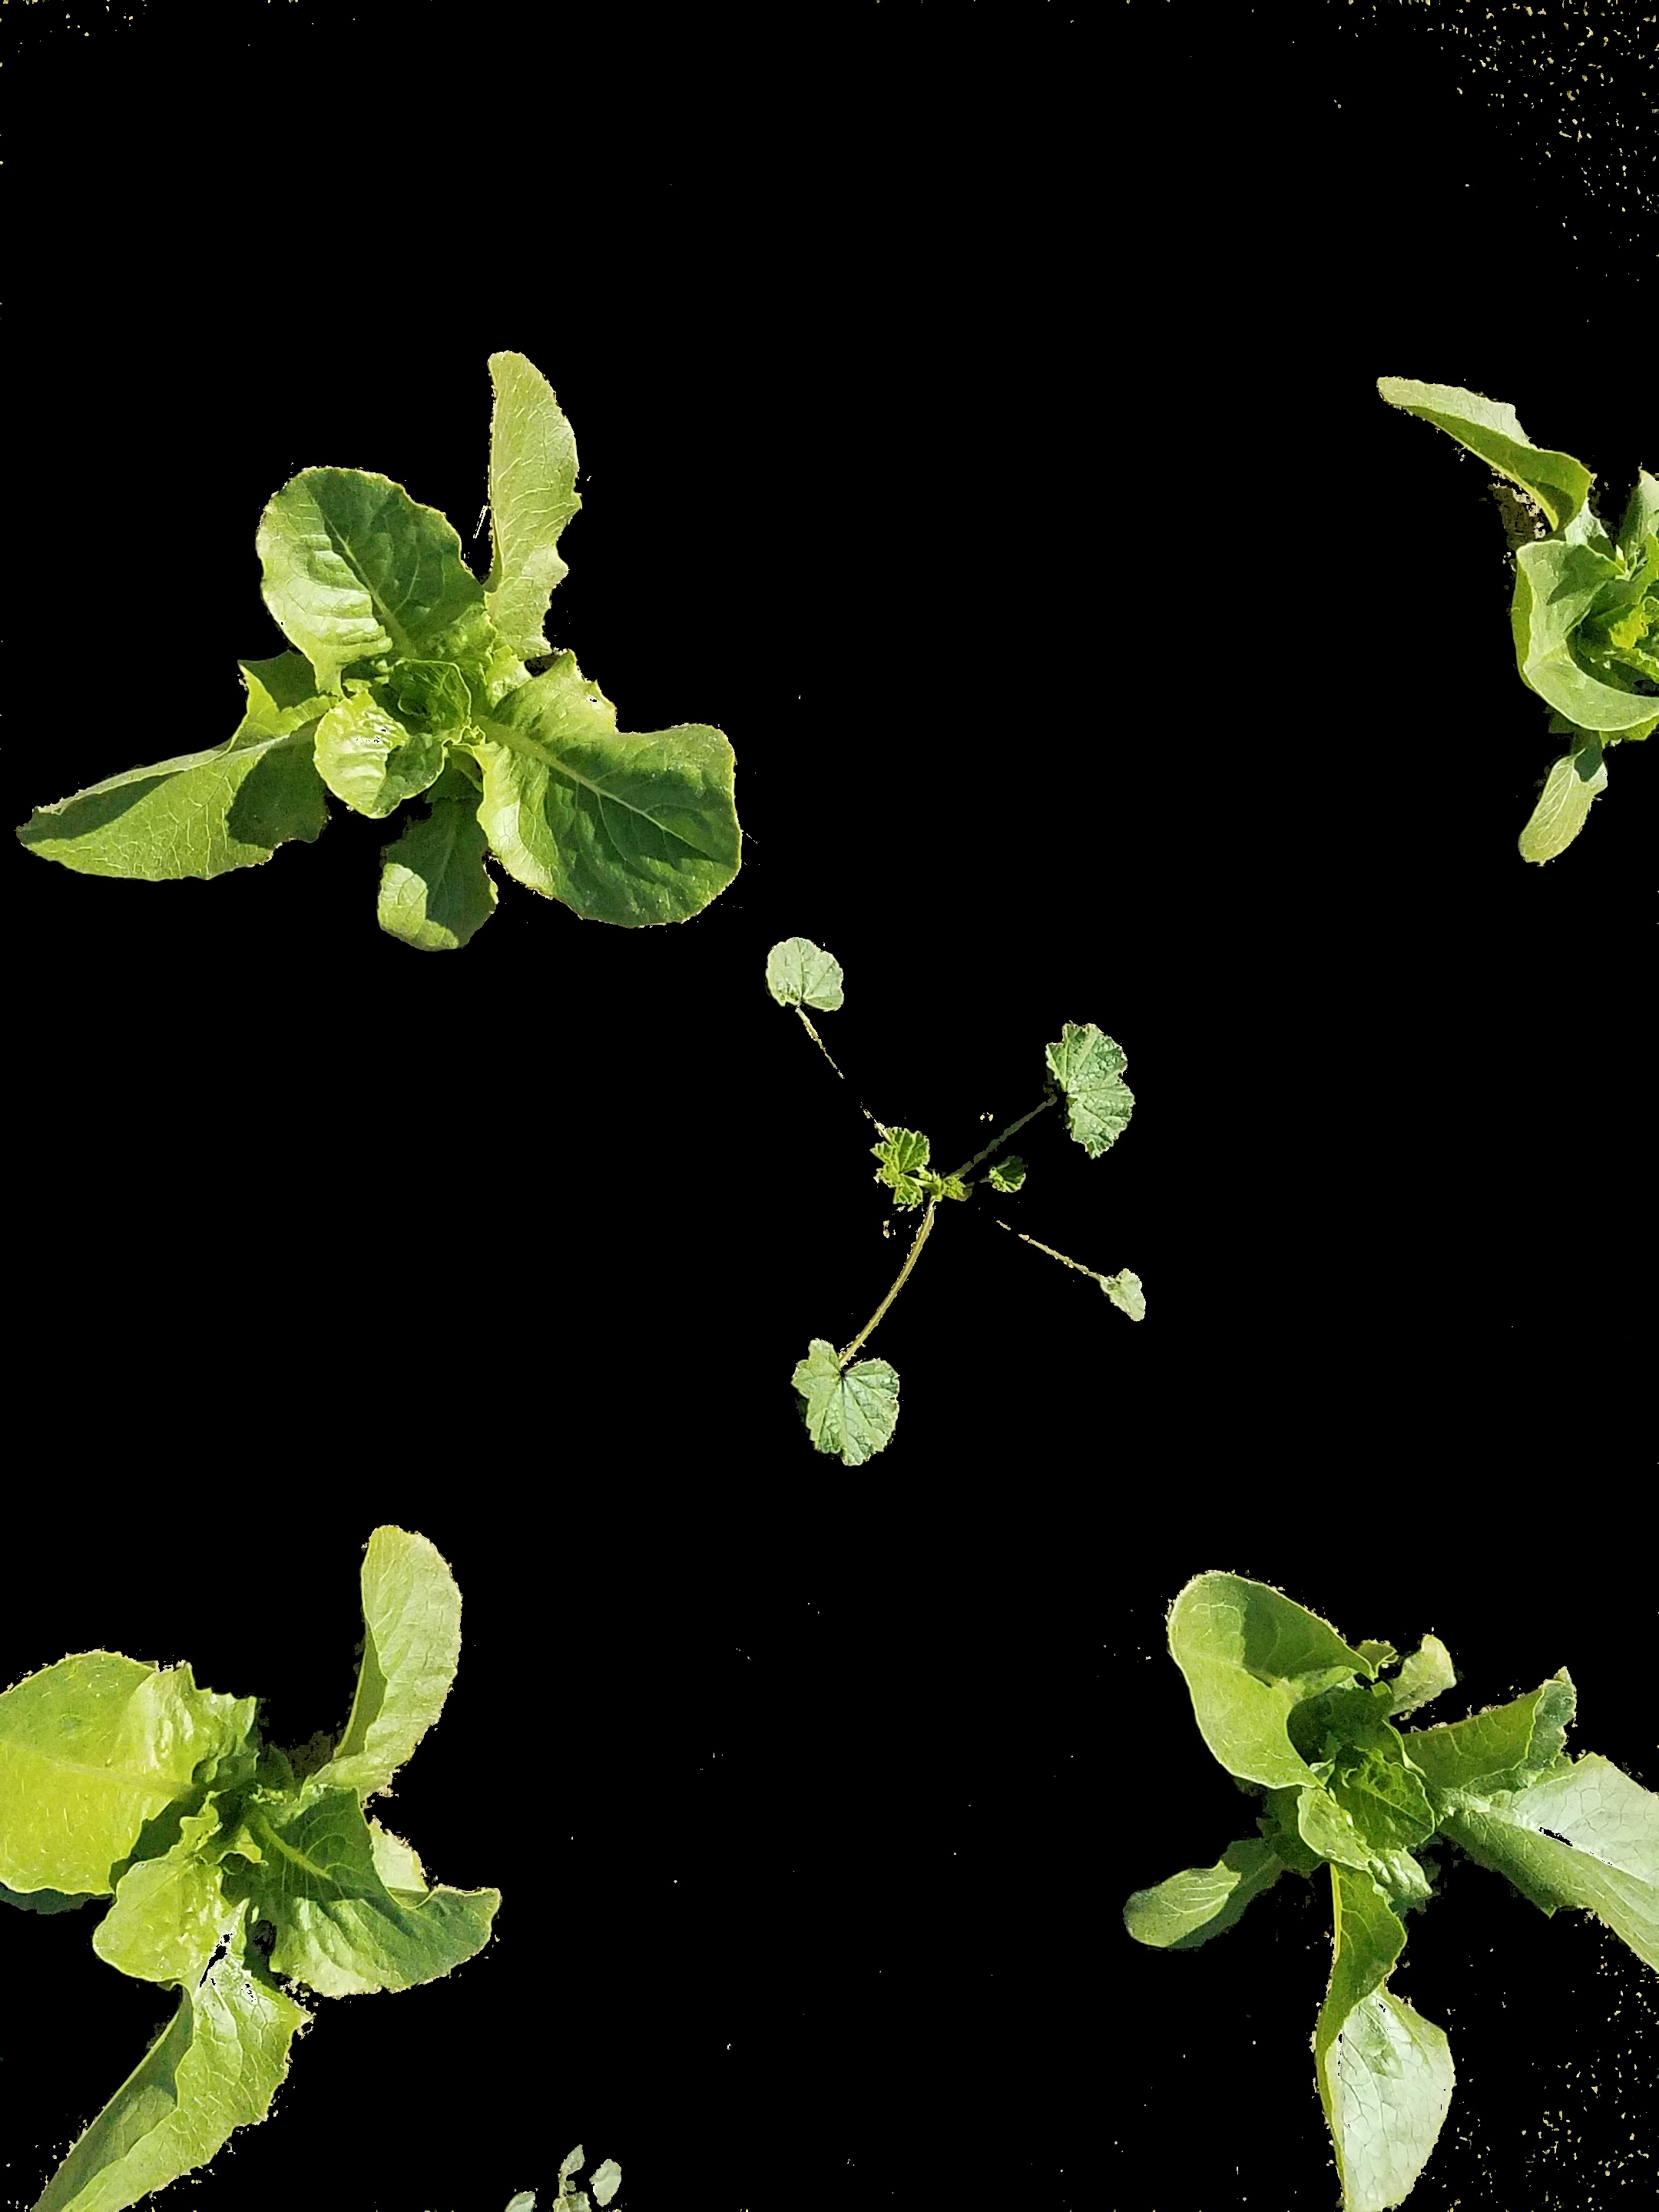
\includegraphics[width = 1.25in]{figures/20201117_112624-YI.jpg} \label{fig:yiq}} &
	\subfloat[Original]{\includegraphics[scale=0.0415,angle=90]{figures/20201117_112624.jpg} \label{fig:original}} \\
	\end{tabular}
	\caption[Segmentation results from various color spaces other than RGB]{Segmentation results from various color spaces outside RGB. The \ref{fig:ci} and \ref{fig:yiq} segmentation approaches are relatively clean, providing vegetation images that are free of ground clutter. The other three approaches, while providing good vegetation images, show too much of the ground, particularly in areas near to a plant, likely due to color contamination in the shadow area.}
	\label{figure:results-color spaces}
\end{figure}

\subsection{Index Evaluation}
Figure \ref{fig:segmentation-errors} shows the error rates encountered with various segmentation techniques, both RGB-centric and those based on other color spaces. Indexing based on the \textit{hue} of the HSI color space produced the best results, the \textit{Excessive Red} (based on RGB) index the worst. Curiously, the index based on the other hue-centric color space, HSV, performed significantly worse. There is no one `correct' index approach, of course. It is more a matter of which sort of error can be tolerated within a system. While the HI approached exhibited the best overall error rate, NGRDI might be a better choice if the false positive error rate is a concern. This work will use the NDI and YCbCr index approaches, as those two indices showed the lowest overall rate.
 
% Bar chart produced with this command
%  python evaluate-masks.py -i ../lib/mask.jpg -t ../lib/testing/20201117_112624
\begin{figure}[h]
	\centering
	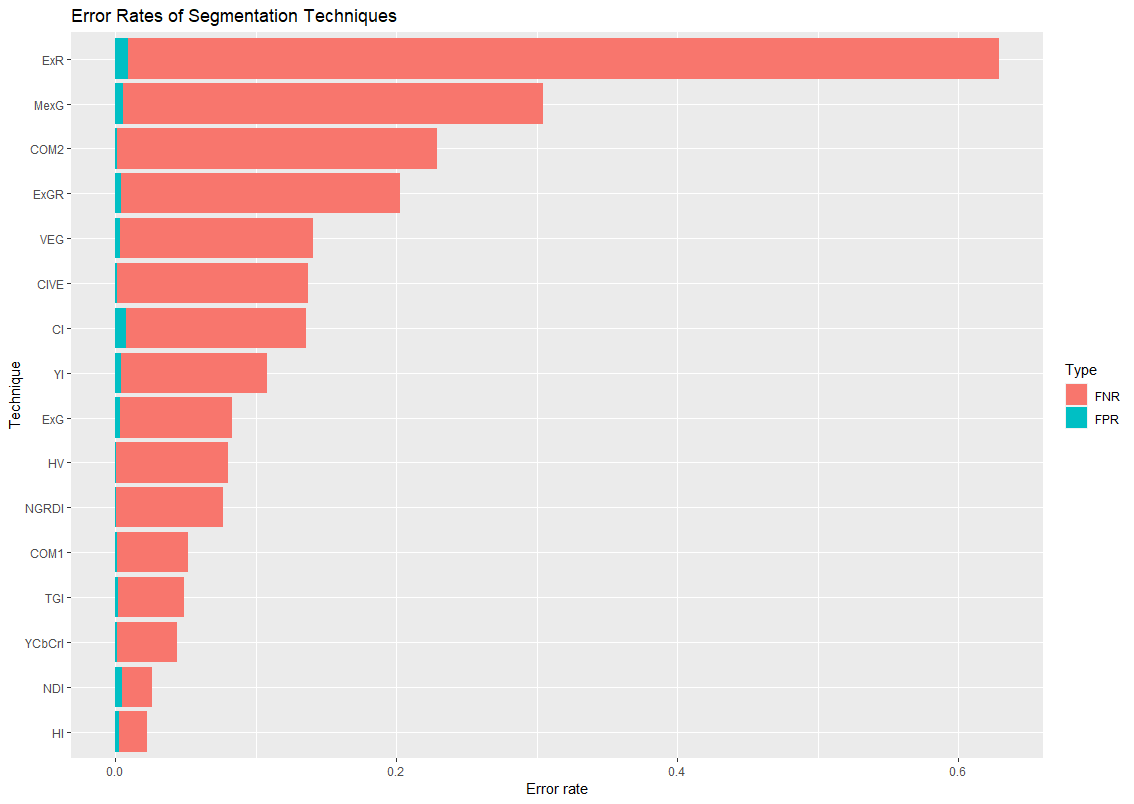
\includegraphics[width=.75\linewidth]{figures/segmentation-error-rates.png}
	\caption[Error rates of segmentation algorithms]{Average error rates for the images. False positive (Vegetation identified as ground) and false negative (Ground identified as vegetation) error are summarized by this figure. Of special note here are the errors encountered with NRGDI and HI approaches, as they represent clear differences in errors. The majority of the errors shown by the HI index mistakenly shows the ground as vegetation, with NDGRI  doing the opposite, hiding vegetation.}
	\label{fig:segmentation-errors}
\end{figure}

\subsubsection{Problem: Reflections and Shadows}
Reflections within vegetation provide a challenge not easily surmounted.  In some cases, the area in reflection is not merely brighter than the surrounding pixels, but is completely devoid of usable pixels, as it is completely white (sometimes referenced as \textit{clipped}). This leads to the situation where portions of the vegetation are not present in the final segmented image, as the pixels do not contain the values associated with vegetation.  Deep shadows within the plant (or shadows produced by one leaf shading another) salso present a similar challenge in that they may be seen as nearly pure black. While mild shadows or reflections do not present much of a challenge, as vegetation in these areas typically have pixel values that are closely associated with their class. Reflections and shadows can be partially mitigated by a technique that improves the overall contrast of the image: \textit{histogram equalization}. Histogram equalization, for lack of a more precise description, stretches out the contrast over a broad range. While histogram equalization cannot reconstruct pixels than have been registered as pure white or pure black, this approach yields images with a more uniform intensity distribution.

Histogram equalization operates by redistributing pixel intensity values across the entire available intensity range, thereby producing a more uniform histogram distribution. Specifically, the technique spreads out the most frequent intensity values, reducing peaks in areas of high concentration and filling in gaps in areas of low concentration. The result is improved visual contrast and increased visibility of features that were previously obscured by shadows, reflections, or varying lighting conditions.


% This produces figures that have aligned captions -- the [t] bit does the trick
\begin{figure}[H]
	\centering
	\subfloat[Leaf with reflection]{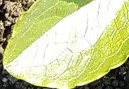
\includegraphics[width=.22\linewidth]{figures/reflection.jpg}\label{fig:leaf-with-reflection}}
	\hfill
	\subfloat[Before]{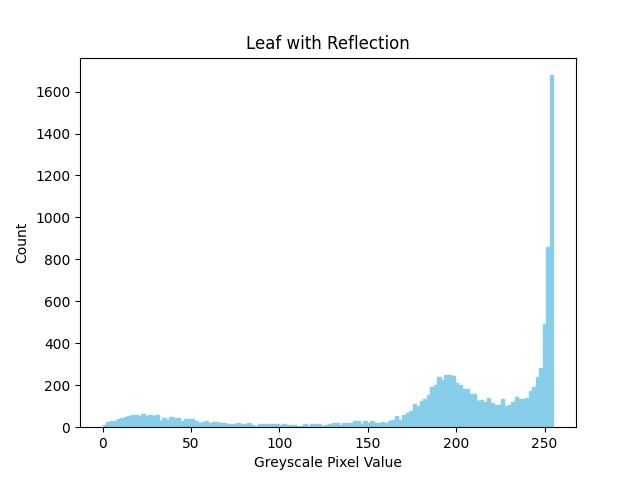
\includegraphics[width=.22\textwidth]{figures/reflection-histogram.jpg}\label{fig:reflection-histogram}}
	\hfill
	\subfloat[After equalization]{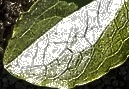
\includegraphics[width=.22\textwidth]{figures/reflection.equalized.jpg}\label{fig:leaf-equalized}}
	\hfill
	\subfloat[After equalization]{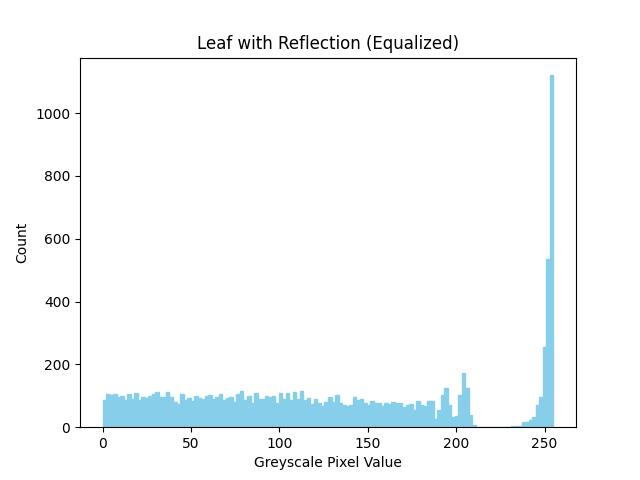
\includegraphics[width=.22\textwidth]{figures/reflection-histogram-equalized.jpg}\label{fig:leaf-equalized-histogram}}
	\caption[Reflection problems in segmented vegetation]{Reflections may be clipped (completely white) containing no usable information. While histogram equalization improves the image somewhat, applying that technique cannot reconstruct pixels that have been recorded as pure white. Figure \ref{fig:leaf-with-reflection} shows a portion of an image with a reflection strong enough to render a significant portion of the image unusable. Note the pixel count for pure or nearly pure white pixels in both \ref{fig:reflection-histogram} and \ref{fig:leaf-equalized-histogram} remain constant.  Those pixels should contain values indicative of vegetation. Aside from being a bit more pleasant to look at, these may have an impact on threshold selection. Note that the histogram of \ref{fig:reflection-histogram} no longer has the same shape, as intensities have be redistributed, eliminating the small bump.}
	\label{fig:reflection}
\end{figure}

\subsubsection{Color problems}
\label{section:problems-color}
Many of the indexes suffer from the same problem: they are focused on vegetation being green. Green stems and leaves are easily detected, but stems and leaves of other colors are not. Consider commonly encountered red-leaf lettuce. Depending on the stage of development and the angle of view, the leaves can be partially or entirely red (or a deep purple color). This is not limited to crops, of course, as weeds such as redroot pigweed (\textit{Amaranthus retroflexus}) have red at the base of the leaves. Likewise, some weeds exhibit red stems. Purslane (\textit{Portulaca oleracea}) has red stems, and as an added complication, red edges on the leaves. Attempts to reveal the stems are complicated by the ground often containing a strong red coloration. Unfortunately, the band of color featured in the stems (red) is frequently found in the background (soil), so attempts to make the stems appear in the masked image are problematic, as this solution tends to bring unwanted ground pixels in the final image that contain hues found within the stems. The result of this is that the non-green portions of the vegetation does not appear in the resulting segmentation.  Even predominately green vegetation has non-green portions. Flowers are often missed by a green-centric index. While the omission of flowers may be desirable in further processing, if the flower obscures green vegetation that would otherwise be identified as such, that complicates further processing, especially when the green portion is significantly obscured. Uncorrected colors also complicate segmentation, as the same plant's leaves may be captured differently with two different cameras or under different lighting conditions. Under controlled lighting conditions (such as would be encountered in an enclosed system) color calibration is not essential every time, but systems that use ambient lighting require calibration each time to achieve optimal results. While the loss of red portions of the plant may not be a significant factor in subsequent processing, this should be taken into account. It may be the case that a single plant appears to be many more, as seen in \ref{fig:ndi}.
There are two other color problems mentioned previously that are worth repeating there. Even green portions of the vegetation may not be green ``enough''. The segmented images in Figure \ref{figure:results} have discarded ground pixels while retaining most of the vegetated pixels that will be used is subsequent processing, but a close examination reveals that pixels in the stems of the weed in the center are also eliminated, as they are less green than the rest of the plant. Likewise, immature vegetation where stems are not sufficiently green will not appear in the final image. The color of a pixel may also be ``contaminated'' with color, as shadows or the edges of shadows may contain the color of the vegetation casting the shadow.
Color problems have profoundly negative effects on index accuracy. Figure \ref{fig:segmentation-color-problem} illustrates this on a single image of Purslane. While this may not ultimately result in errors in forming negative treatment plans, as the identification of a single weed as multiple plants, it may have some effects that are not desirable. More herbicide, for instance, may be applied than is required, given that multiple plants are identified where a single plant exists. Even the calculation of weed population is distorted, reporting the incorrect weed count.


\begin{figure}[H]
	\centering
	\subfloat[Field view of Purslane]{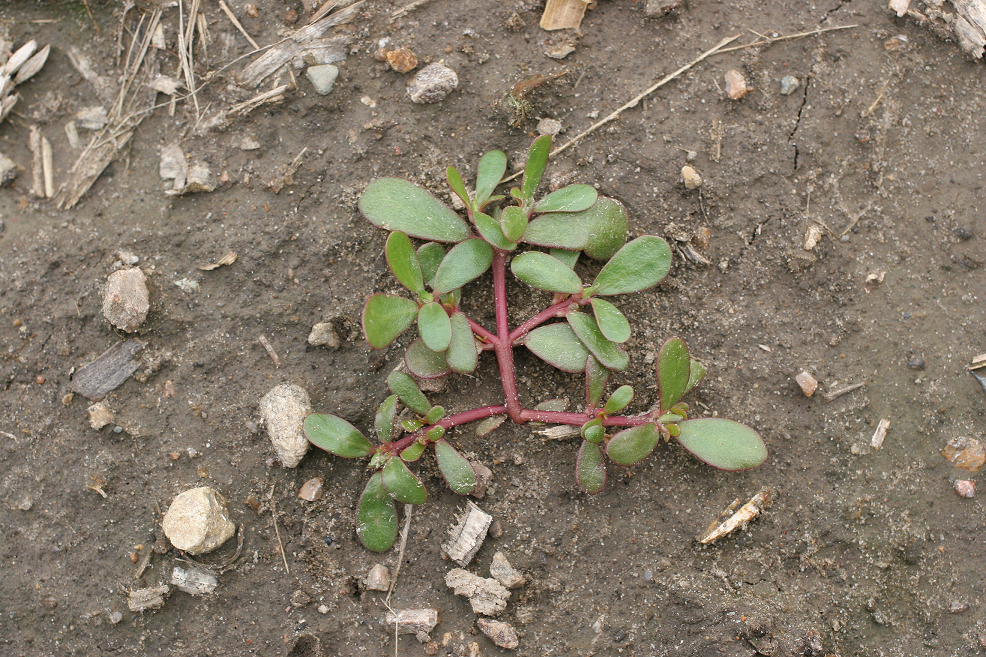
\includegraphics[width=.3\linewidth]{figures/purslane.png}\label{fig:purslane-original}}
	\hfill
	\subfloat[Image processed with NDI]{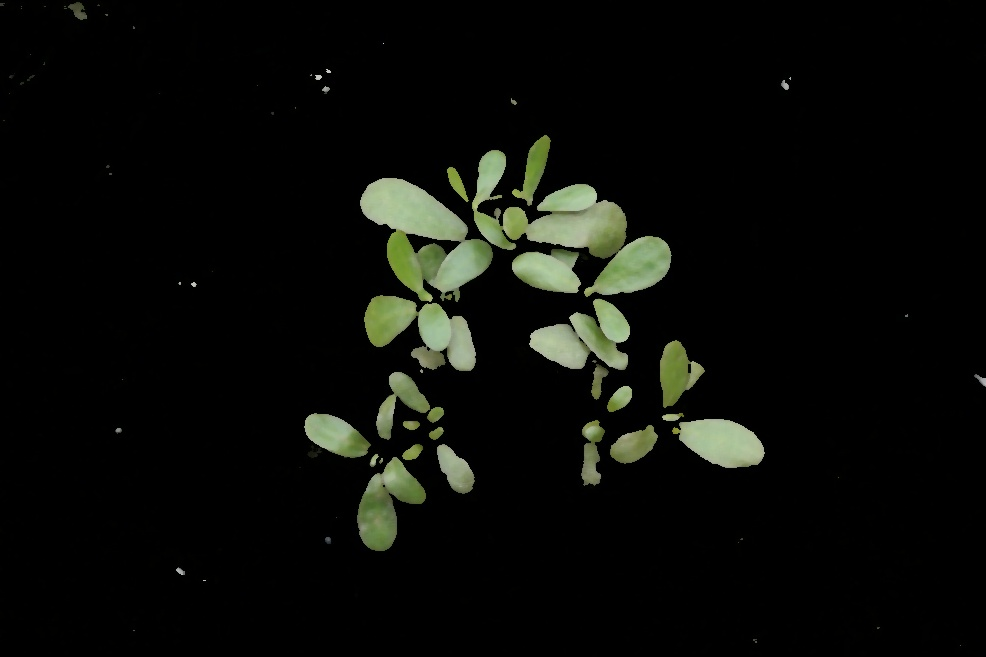
\includegraphics[width=.3\linewidth]{figures/ndi-purslane.jpg}\label{fig:purslane-ndi}}
	\hfill
	% Bar chart produced with this command
	% python evaluate-masks.py -i c:\uofa\weeds\lib\testing\IMG_1133 -s c:\uofa\maricopa\corrected\2024-04-24\iphone-drip\IMG_1133.jpg -t d:\maricopa\masks\2024-04-24\IMG_1133-mask.jpg -l ..\jetson\logging.ini
	\subfloat[Error rates]{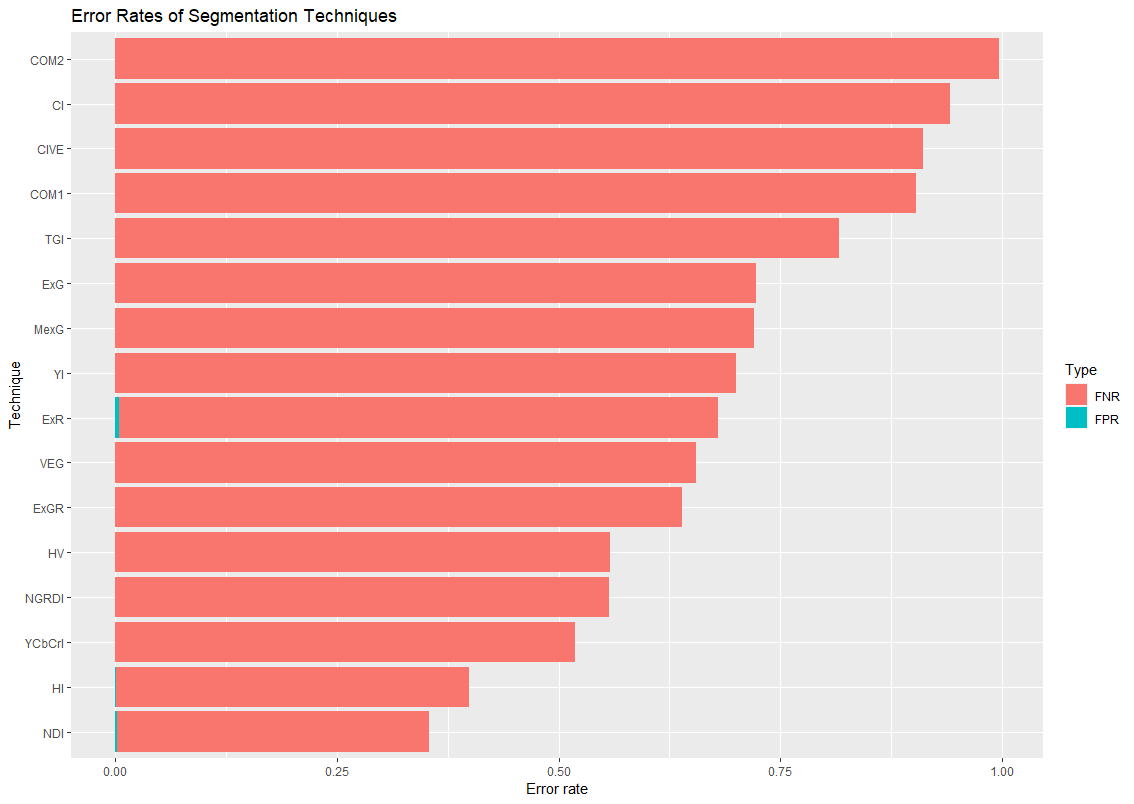
\includegraphics[width=.3\linewidth]{figures/segmentation-error-rates-color.png}\label{fig:error-rates}}
	\caption[Missing red portions of vegetation]{The red portions of the vegetation are missing after the index has been applied, as \ref{fig:purslane-ndi} shows. While the absence of stems may not affect further image processing using factors like leaf texture in classification, the absence of the red portions of features such as leaves may complicate attempts to use factors that are affected such as shape. As \ref{fig:error-rates} shows, the presence of red in a significant portion of the vegetation has a negative impact on the error rates of the algorithms examined.}
	\label{fig:segmentation-color-problem}
\end{figure}

\subsection{Classification Based}
\label{section:classification}
Unlike index-based methods, which rely on straightforward mathematical transformations and thresholding, classification-based approaches utilize machine learning algorithms trained on labeled datasets to determine pixel membership, enabling precise and adaptive segmentation of complex agricultural scenes (this is often referred to as \textit{semantic segmentation}). Table \ref{table:ml-segmentation} shows the results of building models using the following approaches:  Support Vector Machine, Linear Discriminant Analysis, and Multi-layer Perceptron (MLP) (provided in this \textit{scikit-learn} Python package). Each technique was applied to these color spaces: RGB, YIQ, YUV, HSI, HSV, YCbCr, and CIELab. A set of images taken from 2M AGL was selected and 40 samples taken from each of the 58 images, 20 ground points and 20 vegetation points. Figure \ref{fig:color-application} shows a screenshot of the application that was built to collect these samples. The term \textit{samples} in this context means that for each of the points sampled, the values for each of the color spaces identified in Section \ref{section:classification} were recorded. Based on these sample points, models were created and trained on 60\% of the data using the Scikit-learn Python library. While the RGB color space is widely used, using it did not produce the best results for all of the techniques examined. The YIQ space performed better when classifying using MLP. There are some important exceptions to keep in mind, particularly the performance of LDA, where identical scores for both RGB and YIQ spaces are seen. Using these classification approaches is not particularly pragmatic from a realtime perspective, as classifying every pixel in a modest 12MP image can take several hours on a modestly powerful CPU. Given the poor performance in terms of compute time of this technique, it will not be considered for this project.

\begin{figure}[H]
	\centering
	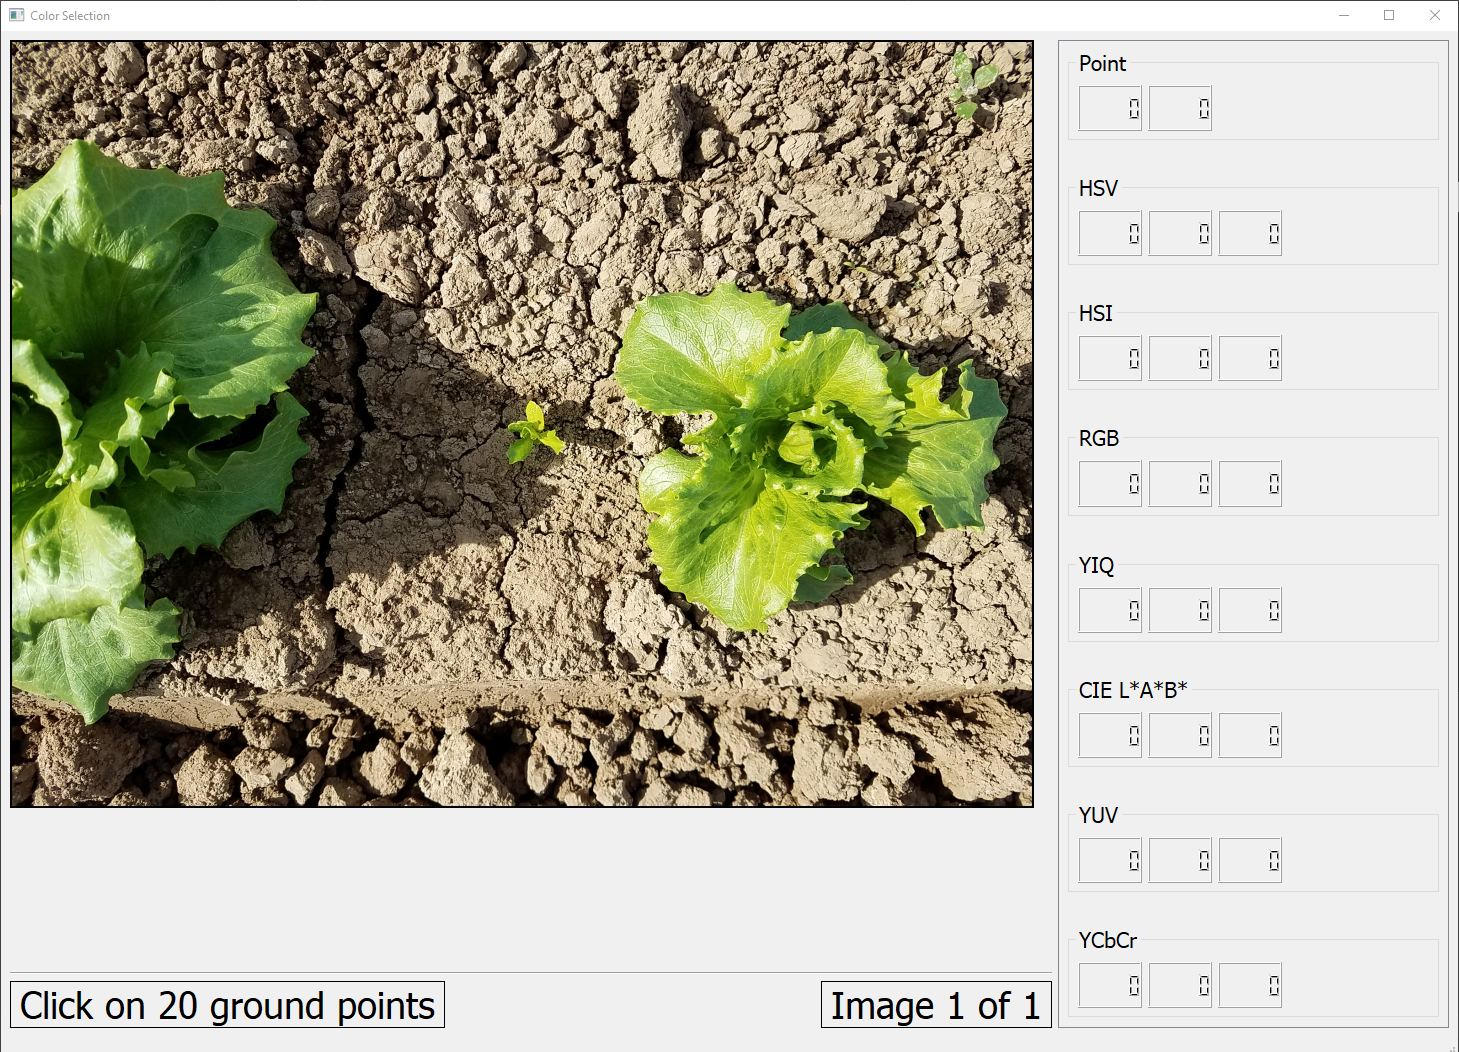
\includegraphics[scale=0.30]{./figures/color-screenshot.png}
	\caption[Color sampling UI]{This application allows a specified number of ground and vegetation points to be sample for each image in a set. The color values along the left-hand side of the interface are simply for debug purposes, not for user interaction. Users simply click on the specified number of ground and vegetation points, and the image automatically advances through the set.}
	\label{fig:color-application}
\end{figure}

%
% Begin Copied Table from this command
% python segment.py -i images -o segmented -t ../util/segmentation-training.csv  -b -s -l logging.ini -a all
% Minor manual edit: Remove leading space from header lines

Table \ref{table:ml-segmentation} shows a summary of the three classification approaches in various color spaces, giving the Area Under the Curve (AUC), Precision, Recall, and F1 scores. And while the the scores reported are encouraging, the time taken to produce the resulting segmented images is not. Some of the techniques required hours to process a high-resolution image. Even with optimization and reduced-resolution images, it is unlikely that any of these classification techniques would be appropriate for use in a real-time system.

% Spacing between the rows
{
\renewcommand*{\arraystretch}{0.89}

%
% Begin Copied Table from this command
% python segment.py -i images -o segmented -t ../util/segmentation-training.csv  -b -s -l logging.ini -a all
% Minor manual edit: Remove leading space from header lines & data


\begin{longtable}{llrrrr}
\caption[Machine Learning Segmentation]{Machine Learning Segmentation}
\label{table:ml-segmentation}\\
\toprule
Technique &  Color &  AUC & Precision & Recall &   F1\\
\midrule
\endfirsthead
\caption[]{Machine Learning Segmentation} \\
\toprule
Technique &  Color &  AUC & Precision & Recall &   F1\\
\midrule
\endhead
\midrule
\multicolumn{6}{r}{{Continued on next page}} \\
\midrule
\endfoot

\bottomrule
\endlastfoot
MLP &RGB & 0.93 &      0.88 &   0.95 & 0.91 \\
MLP &YIQ & 0.94 &      0.88 &   0.96 & 0.92 \\
MLP &YUV & 0.94 &      0.88 &   0.96 & 0.92 \\
MLP &HSI & 0.91 &      0.86 &   0.94 & 0.90 \\
MLP &HSV & 0.90 &      0.87 &   0.94 & 0.91 \\
MLP &YCBCR & 0.94 &      0.88 &   0.96 & 0.92 \\
MLP &CIELAB & 0.94 &      0.88 &   0.96 & 0.92 \\
LDA &RGB & 0.94 &      0.88 &   0.96 & 0.92 \\
LDA &YIQ & 0.94 &      0.88 &   0.96 & 0.92 \\
LDA &YUV & 0.94 &      0.88 &   0.96 & 0.92 \\
LDA &HSI & 0.91 &      0.86 &   0.95 & 0.90 \\
LDA &HSV & 0.90 &      0.86 &   0.95 & 0.90 \\
LDA &YCBCR & 0.94 &      0.88 &   0.96 & 0.92 \\
LDA &CIELAB & 0.94 &      0.88 &   0.96 & 0.92 \\
SVM &RGB & 0.94 &      0.89 &   0.96 & 0.92 \\
SVM &YIQ & 0.92 &      0.88 &   0.82 & 0.85 \\
SVM &YUV & 0.93 &      0.86 &   0.93 & 0.89 \\
SVM &HSI & 0.91 &      0.87 &   0.94 & 0.90 \\
SVM &HSV & 0.90 &      0.87 &   0.94 & 0.90 \\
SVM &YCBCR & 0.92 &      0.85 &   0.91 & 0.88 \\
SVM &CIELAB & 0.91 &      0.86 &   0.96 & 0.90 \\
\end{longtable}

% 
% End copied table
%
}

\subsection{Semantic Segmentation}
Semantic segmentation is a convolutional neural network (\gls{CNN}) using a trained model to classify each pixel in an image with a class label.  For the most part, crop images contain only two classes: plants and the ground. While there are exceptions to this,  as images may include debris on the ground, irrigation equipment, etc.  The focus here remains to produce a mask that can be applied to the image to isolate vegetated pixels and speed up and make more accurate the actual weeds identification. This approach differs from the prior two approaches in that while index-based approaches consider no information about other images, and learning base approaches consider samples of a set of images to predict class membership, the deep-learning techniques considered in this section are trained on both images and the corresponding masks.

\subsubsection{U-Net}
The name of the U-Net architecture derives from the U-shaped arrangement of the downward decoder section and the upward encoder section. Developed initially for the segmentation of bio-medical images \parencite{Ronneberger2015-ye}, this technique has been more widely adopted into various use cases. The U-Net architecture is characterized by its U-shaped structure, which gives it its name. It consists of an encoding path and a decoding path.
\begin{itemize}
	\item{Encoding Path: This part of the network captures the context of the input image by using a series of convolutional and max-pooling layers to downsample the spatial dimensions. It “contracts” the original images.}
	\item{Decoding Path: The decoding path uses upsampling and convolutional layers to produce a segmentation map that has the same spatial dimensions as the input image. It “expands” the contracted images.}
\end{itemize}

\begin{figure}[H]
	\centering
	\includegraphics[height=5cm]{figures/u-net-architecture.png}
	\label{fig:u-net}
	\caption[U-Net architecture]{The name of U-Net architecture refers to the arrangement of decoders (often referred to as a contracting path) and encoders (the expanding path)}
\end{figure}
This architecture has a bit of a limitation that must be taken into account in image sets: the length of each image's axis must be a multiple of 16. That is, a 32x32 image will work, but a 32x90 image will not. The images and masked used for training and testing should be resized to fit this limitation. Additionally, the images must be down-sampled to achieve realistically short mask production times. (That is, the images were 1008x752 instead of the original 4032x3024) Using a model trained on images and associated masks from the MAC to a set of test images yields fairly low error rate masks when  those masks are evaluated against the ground truth: FPR of 0.0005 and FNR of 0.06, comparable to the lower rates achieved with some index-based approaches.

\begin{figure}[H]
	\centering
	\subfloat[Ground truth mask]{\includegraphics[width=.3\linewidth]{figures/IMG_1115-mask.jpg}}
	\label{fig:unet-original}
	\hfill
	\subfloat[U-Net mask]{\includegraphics[width=.3\linewidth]{figures/IMG_1115-mask-unet.png}}
	\label{fig:unet-mask}
	\hfill
	\subfloat[Apply U-Net mask]{\includegraphics[width=.3\linewidth]{figures/IMG_1115-original-masked.png}}
	\label{fig:unet-original-masked}
	\caption[U-Net segmentation vs ground truth]{The mask produced with U-Net shows some errors within the leaf, but is quite close to a match for the ground truth.}
	\label{fig:u-net-segmentation}
\end{figure}


\section{Blob Identification}
Segmented tend to yield images with  vegetated pixels that are at times not separated. Single items within those images are often called \textit{blobs}, and as that is the term generally used by the OpenCV image processing software libraries, that is the term adopted for this document. Blobs are the largest area of contiguous pixels with non-zero values.  The mask produced in the previous section requires some further refinement with morphological operations \textit{dilation} and \textit{closing} before it can be used, as the mask produced using only the index tends to hide portions of the vegetation. Dilation is an operation that “grows” or “expands” objects in a binary or grayscale image. It works by sliding a structuring element (a predefined shape, such as a square or circle) over the image and replacing the pixel under the center of the structuring element with the maximum value covered by the structuring element (in grayscale images) or by setting the pixel to 1 (in binary images) if any pixel under the element is 1. Closing is a compound operation that consists of a dilation followed by an erosion, using the same structuring element for both operations. The dilation step first expands the object boundaries, and the erosion step then shrinks them back. This combination smooths the contours of objects, closing small holes and gaps without significantly altering the overall shape.

\begin{figure}[h!]
	\centering
	\begin{subfigure}[h]{.48\textwidth}
	  \centering
	  \includegraphics[height=5cm]{./figures/mask-raw.jpg}
	  \caption{Unrefined mask}
	  \label{fig:mask-raw}
	\end{subfigure}
	\hfill
	\begin{subfigure}[h]{.48\textwidth}
	  \centering
	  \includegraphics[height=5cm]{./figures/mask-processed.jpg}
	  \caption{Mask refined with pixel dilation and closing}
	  \label{fig:mask-processed}
	\end{subfigure}
	\caption[Mask before and after morphological refinements]{The unprocessed and refined mask. The unrefined mask in Figure~\ref{fig:mask-raw} would not allow for many of the details of the plant to be present in the final image. Note that large portions of some of the leaves are rendered  black, even as the vegetation edges are not. After the pixels are dilated with a 5x5 kernel of all 1s, the mask shown in Figure~\ref{fig:mask-processed} is produced, allowing all pixels within the leaf area to be present in the final image.}
	\label{fig:mask-before-and-after}
\end{figure}


Figure~\ref{fig:original-masked} shows an image with  eight blobs that can be classified: three lettuce plants and a single weed plant that appears as five plants in the final image.

\section{Feature Extraction}
Once the vegetation is isolated and blobs identified, various features can be extracted for subsequent use in classification. These features include position-independent characteristics such as shape, hue, and textural characteristics as well as position-dependent features such as where a plant resides relative to the crop-line and size ratios between objects.  

\subsection{Shape Characteristics}
The shape of an object can be globally or locally described by various factors \parencite{Zhang2004-cm}. The problem quickly encountered in using shape in this instance is that a 3D object is projected on to a 2D plane, losing information in the process. The object in the resulting image is, of course, only a partial representation of the object as it exists in the real world. As section \ref{problem-overlap} shows in greater detail, even simple, but common occurrences such as object overlap complicate attempts to exploit shape. The classification examined in this work will consider only the former, global descriptors that apply to an entire object. Shape parameters used in classification must exhibit three characteristics: scale invariance, rotation invariance, and translation invariance. Rotation invariance is, perhaps, the most relatable of these. While a camera mounted on a UAV or tractor will collect imagery in the same orientation, plants are not so obliging in orientation of their growth. Two plants might have leaves that may look extremely similar (and could be said to be of the same shape), but are rotated by 90\si{\degree}. Scale invariance is almost as easy to describe: two leaves have the same shape, but are simply of different size due to differences in the time of emergence. Translation invariance means that the same descriptor is derived without considering the position of the object within the image.  A fourth invariance is a bit more complex: viewpoint. While a camera capturing images as it passes overhead can always -- within a very small variation -- be considered to have the same viewpoint, the same does not hold true for the plants in the image. Two leaves can have the same physical shape, but differences in orientation with respect to the Z-axis (consider the case where the tip of one leaf is closer to the ground) produce significantly different descriptions of their shape. While a perfect shape descriptor would be invariant under all of these, it is typically not realistic to arrive at a shape descriptor that is invariant in all cases.
The shape parameters considered in this analysis are expressions describing the perimeter of the plant. The formulae used to extract the various shape features are given in Table~\ref{tab:shape-formulae}.

\subsubsection{Shape Basics}
Here it may be necessary to discuss two topics that will appear is some of the details that follow: \textit{perimeter}, and \textit{major$/$minor axis}. The perimeter of an object, in this context, consists of the set of pixels that form the boundary of an object. An example perimeter is shown in \ref{fig:bounding-box}. The blue pixels following the edge of the plant define the perimeter. While the perimeter is a simple concept, the major and minor axes are more complex. The major axis is the longest line that can be drawn through an object. If two objects of equal area are considered, one circular and one oval, the oval will have a longer major axis. The minor axis is considered to be the longest line that can be drawn perpendicular to the major axis.

\begin{figure}[h!]
	\centering
	\includegraphics[scale=0.5]{./figures/shape-major-minor.png}
	\caption[Major/Minor Axis]{The major/minor axis of an object are illustrated by this simple example using an oval. The major axis is the longest line that can be drawn though the oval, and the minor axis is the longest line that can be drawn perpendicularly though that axis.}
	\label{fig:major-minor}
\end{figure}


\subsubsection{Bounding Box and Convex Hull}
An object can be said to have rectangular box of minimum size that completely encloses the object, commonly termed the \textit{bounding box}. The box placed around the object without regard for orientation -- that is, the placement makes no attempt to align the edges of the box with the edges of the image, so it may appear tilted at normal viewing angles. The \textit{convex hull}, likewise, is a convex shape with straight lines and of minimum size that completely encloses the object.   
\begin{figure}[h!]
	\centering
	\begin{subfigure}[h]{.48\textwidth}
	  \centering
	  \includegraphics[height=5cm]{./figures/shape-bounding-box.jpg}
	  \caption{A bounding box}
	  \label{fig:bounding-box}
	\end{subfigure}
	\hfill
	\begin{subfigure}[h]{.48\textwidth}
	  \centering
	  \includegraphics[height=5cm]{./figures/shape-convex-hull.jpg}
	  \caption{A convex hull}
	  \label{fig:convex-hull}
	\end{subfigure}
	\caption[Bounding box and convex hull]{A bounding box and a convex hull (both noted in green) surround an object, but a convex hull is a shape with the minimum size that can contain the object. A bounding box is the minimum sized rectangle that can contain the object.}
	\label{fig:bounding-and-hull}
\end{figure}
The convex hull is a simple polygon whose vertices are a subset of the points found in the edge of the original shape. A widely used algorithm for determining the convex hull, \textit{Graham's Scan} is fairly efficient, $\mathcal{O}(n\log n)$, as \citeauthor{Klette2004-qz} show in this excerpt (altered for clarity with assistance from lecture notes from \citeauthor{Prosser1998-mi}). \parencite{Klette2004-qz}
\begin{quote}
\begin{enumerate}
	\item{Find the bottom-most point by comparing \textit{y} coordinate of all points. If there are two points with the same \textit{y} value, then the point with smaller \textit{x} coordinate value is considered. Let the bottom-most point be $P0$. Put $P0$ at first position in output hull.}
	\item{Sort the remaining points $p_i$ of $S$ in order of increasing angles $\eta_i$; if the angle is the same for more than one point, keep only the point furthest from $p$. Let the resulting sorted sequence of points be $q_i,..., q_m$.}
	\item{Initialize $C(S)$ by the edge between $p$ and $q_1$.}
	\item{Scan through the sorted sequence. At each left turn, add a new edge to $C(S)$; skip the point if there is no turn (a collinear situation); backtrack at each right turn.}
\end{enumerate}
\end{quote}
The most salient problem with the convex hull, however, is one that will have an adverse affect on all shape descriptors: distortions introduced by the resolution of the same object at different altitudes. That is, the edges are described by fewer pixels as the distance between the camera and plant increases, resulting in increased pixelation. While this can be minimized to some extent by blurring the image prior to performing the hull calculations, the hull is still distorted by this lower resolution.

\subsubsection{Area \& Size Ratio}
The area of the plant in the segmented image is simply the number of pixels with non-zero values. The term \textit{area} in this context is considered only in terms of pixels, not how much the pixel captures of the ground (e.g., the $cm^2$ each pixel represents). The relative area of two plants can then be compared to predict membership in a class. For instance, if a plant is $\frac{1}{3}$ the size of the largest plant in the image it is more likely than not a weed. This ratio is highly dependent on the development phase of the crop, as the reverse could be true for crop just emerging compared to much larger weeds. For the classification purposes presented here, the larger item is presumed to be crop.

% Figure produced with this command
% make weeds-no-db INPUT=/cygdrive/d/dissertation/ OUTPUT=/cygdrive/d/dissertation/output/ TRAINING=/cygdrive/d/maricopa-test/imbalance/processed/final/corrected.csv THRESHOLD=TRIANGLE INDEX=com2 DECORATIONS=area SESSION=shape
\begin{figure}[h!]
	\centering
	\includegraphics[height=4cm]{./figures/shape-area.jpg}
	\caption[Shape attribute: Area \& Size Ratio]{The area of the object in terms of numbers of pixels. By itself, this is not a particularly useful metric, but it may be useful to consider the relative sizes of plants to each other. As can be seen in this example, the crop plant is several times the size of the weed. This is, of course, highly dependent on the phase of development and how long the weed has been allowed to grow.}
	\label{fig:shape-area}
\end{figure}

\subsubsection{Length/Width Ratio}
\label{sec:length-width-ratio}
The ratio of width to length is not -- as the name might imply -- a simple ratio of two measurements, but is expressed as:
\begin{equation}
S = 
	\begin{bmatrix}
	Var(X) & Cov(XY) \\[0.3em]
	Cov(XY) & Var(Y) \\[0.3em]
	\end{bmatrix},
\lambda = \frac {eig_{1}(S)} {eig_{2}(S)}
\end{equation}
Where $eig_{1}(S)$ and $eig_{2}(S)$ are the maximum eigenvalues of the matrix $S$, with $\lambda$ representing the ratio. (\cite{Lin2017-xq}) The X and Y positions refer to an object's perimeter -- the boundary between an object's edge and the background.

% Figure produced with this command
%  make weeds-no-db INPUT=/cygdrive/d/dissertation/ OUTPUT=/cygdrive/d/dissertation/output/ TRAINING=/cygdrive/d/maricopa-test/imbalance/processed/final/corrected.csv THRESHOLD=TRIANGLE INDEX=com2 DECORATIONS=lw_ratio SESSION=shape

\begin{figure}[h!]
	\centering
	\includegraphics[height=4cm]{./figures/shape-lw-ratio.jpg}
	\caption[Shape attribute: Length-Width ratio]{The length-width ratio of plants. Note that the length-width ratio of the plant on the left of the image cannot be determined, as it is cut off, a common occurrence in images.}
	\label{fig:shape-area}
\end{figure}

\subsubsection{Boundary Descriptors}
There are two global descriptors of an object's edge that are used here: the bending energy and the radial distance. Describing the bending energy of an object involves a few preliminary steps. Changes in the $(x,y)$ position of edge pixels can be described by a \textit{chain code}. A chain code representation of a boundary describes unit length changes in the $(x,y)$ positions of the boundary,  where changes in the position are noted by their position in a matrix:

 \begin{figure}[h!]
	\centering
	\begin{subfigure}[h]{.4\textwidth}
	  \centering
	  \includegraphics[height=3cm]{./figures/chain-code-matrix.jpg}
	  \caption{Chain code matrix}
	  \label{fig:chain-code-matrix}
	\end{subfigure}
	%\hfill
	\begin{subfigure}[h]{.4\textwidth}
	  \centering
	  \includegraphics[height=3cm]{./figures/chain-code-cells.jpg}
	  \caption{Example edge}
	  \label{fig:chain-example}
	\end{subfigure}
%	\hfill
%		\begin{subfigure}[h]{.25\textwidth}
%	  \centering
%	  \includegraphics[height=2cm]{./figures/chain-code-result.jpg}
%	  \caption{Result}
%	  \label{fig:chain-result}
%	\end{subfigure}
	\caption[Boundary chain codes]{Chain codes of the transitions of an object's edge -- as seen in successive pairs of coordinates -- are described by positions within an 8 position matrix, with each position noting the change in the $(X, Y)$ coordinate (steps of length 1 along the $x,y$ axis lines and of length $\sqrt{2}$ for diagonal movements). In this example the edge has a chain code of 2,1,0,7,7,0,1,1. While this example shows an open curve with a distinct beginning and ending, the boundary of a plant is a closed curve with no distinct end or beginning. A 4 direction matrix is also used, as is a general $N$-directional chain $(N > 8\ and\ N =2^k)$, although those variants are not addressed in this work. The 8 position matrix is, perhaps, the most relatable, as changes in adjacent boundary pixels always take one of the 8 possibilities present in the matrix. The matrix shown in \ref{fig:chain-code-matrix} is a $3x3$ matrix, but the middle position (implying no change) is not possible -- this is simply an illustration.}
	\label{fig:chain-codes}
\end{figure}

The \textit{$\kappa$-slope} of a given boundary point $(X_i, Y_i)$ is estimated from the slope of the line joining positions $(X_{i-k/2}, Y_{i-k/2})$ and $(X_{i+k/2}, Y_{i+k/2})$ with this equation:
\begin{equation}
\tan^{-1}\left(\frac{Y_{i+k/2} - Y_{i-k/2}}{X_{i+k/2} - X_{i-k/2}}\right)
\end{equation}
 
 The \textit{$\kappa$-curvature} of the boundary at location $(X_i,Y_i)$ can be estimated by this equation:
 \begin{equation}
 \tan^{-1}\left(\frac{Y_{i+k} - Y_{i}}{X_{i+k} - X_{i}}\right) - \tan^{-1}\left(\frac{Y_{i} - Y_{i-k}}{X_{i} - X_{i-k} }\right)
 \end{equation}
 The goal of this metric is to assess the concavity or convexity of points along the perimeter. Consider the weed in Figure \ref{fig:curvature-weed} with the computed $\kappa$-curvature.
 
  \begin{figure}[h!]
	\centering
	\begin{subfigure}[h]{.4\textwidth}
	  \centering
	  \includegraphics[height=4cm]{./figures/for-curvature-blob-1.jpg}
	  \caption{Weed}
	  \label{fig:curvature-weed}
	\end{subfigure}
	%\hfill
	\begin{subfigure}[h]{.4\textwidth}
	  \centering
	  \includegraphics[height=4cm]{./figures/curvature-blob-1.jpg}
	  \caption{$\kappa$-curvature}
	  \label{fig:curvature-plot}
	\end{subfigure}
	\caption[Example of $\kappa$-curvature]{The $\kappa$-curvature of various points around the perimeter of the weed are illustrated here. Positive values are indicative of convex shapes. Likewise, negative values indicate concave shapes.  While it is tempting to relate the values shown in the graph to the image displayed (as the figure invites the user to do), exact correlation is not advised, as the points sampled may not match the finer details that can be seen in the leaf. This example uses a relatively coarse sampling. However, the image does show a pronounced curve at the lower edge that can be seen in the curvature plot.}
	\label{fig:curvature}
\end{figure}
This leads to a global descriptor used in classification: \textit{bending energy}. Bending energy is typically described as the energy required to bend a rod to the shape under consideration, and is expressed as the sum of squares of the $\kappa$-curvature over the boundary length $L$.
\begin{equation}
\frac{1}{L} \sum_{p=1}^{L}\kappa(p)^2
\end{equation}
While there will be no bending of rods required for classification, this global metric can be used to express the overall shape of the perimeter, exploiting the fact that weeds in a crop and the crop itself exhibit different shapes.

% Figure produced with this command
%  make weeds-no-db INPUT=/cygdrive/d/dissertation/ OUTPUT=/cygdrive/d/dissertation/output/ TRAINING=/cygdrive/d/maricopa-test/imbalance/processed/final/corrected.csv THRESHOLD=TRIANGLE INDEX=com2 DECORATIONS=bending SESSION=shape

\begin{figure}[h!]
	\centering
	\includegraphics[height=4cm]{./figures/shape-bending.jpg}
	\caption[Shape attribute: Bending Energy]{The bending energy}
	\label{fig:shape-bending}
\end{figure}

The \textit{radial distance} can also be used to describe the shape. \citeauthor{Kilday1993-aq}, in a study of classification of lesions in mammogram images, describe techniques to exploit the radial distance of a shape \parencite{Kilday1993-aq}. To understand the principles of radial distance, let’s look at the object in Figure \ref{fig:radial-distance}
\begin{figure}[H]
	\centering
	\includegraphics[width=.25\linewidth]{./figures/radial-distance.jpg}
	\caption[Radial distance from object centroid]{The radial distance from object centroid is noted by \textit{d} in this figure. Scale invariance is achieved by expressing functions of the normalized distance (using the maximum radial distance of the object).}
	\label{fig:radial-distance}	
\end{figure}
As Figure \ref{fig:radial-distance} shows, the radial distance referred to is the distance from an object's centroid (geometric center) to its perimeter $(x,y)$ locations. To make this distance scale invariant, the normalized distance to the maximal distance is used. Using the normalized radial distance, the mean and standard deviation is given by these equations for the $i^{th}$ blob:
\begin{equation}%\labeleqn{Radial distance mean and standard deviation}
\bar{x}_i = \frac{1}{N}\sum_{k=1}^{N}r_k \qquad
\sigma_i = \sqrt{\frac{1}{N}\sum_{k=1}^{N}({r_k} - \bar{x}_i)^2}
\end{equation}
By themselves these metrics may not be particularly useful in predicting class membership, however these provide useful information for metrics that may be. The number of times the normalized radial distance crosses the mean, for instance, provides an estimate of the roughness of a perimeter. So while the radial distance is not used directly, it is used indirectly as a roughness metric in subsequent processing.


% Begin table of shape equations
\begin{longtable}{x{\dimexpr.15\columnwidth-2\tabcolsep}
                  x{\dimexpr.425\columnwidth-2\tabcolsep}
                  x{\dimexpr.425\columnwidth-2\tabcolsep}}
%\begin{hyphenrules}{nohyphenation}
    \caption{Shape Features}\label{tab:shape-formulae}  \\
\toprule
{\textbf{Feature}} & {\textbf{Formula}} & {\textbf{Comment}}
\tabularnewline
\midrule
    \endfirsthead
%%%%
    \caption{Shape Features (cont.)}\label{tab:shape-formulae}  \\
\toprule
{\textbf{Feature}} & {\textbf{Formula}} & {\textbf{Comment}}
\tabularnewline
\midrule
    \endhead
%%%%
\midrule[\heavyrulewidth]
\multicolumn{3}{r}{\footnotesize\itshape
                   Continued on the next page}
    \endfoot
%%%%
\bottomrule
    \endlastfoot
%%%%
		Perimeter
		& \begin{minipage}[t]{0.3\textwidth}
			$\sum_{i=1} ^{N-1}\left|X_1 - X_{i+1}\right| $
		   \end{minipage}     
		& Count of pixels forming the boundary of an object
\tabularnewline\addlinespace

		Major/Minor Axis     
		& $\sqrt{(x_2 - x_1)^2 + (y_2 - y_1)^2} $                    
		& Major axis is the longest line that can be drawn through the object. Minor axis is the longest line that can be drawn through the object such that the line remains perpendicular to the major axis.
\tabularnewline\addlinespace

		Compactness      
		& \begin{minipage}[t]{0.3\textwidth}
			$\frac{4\pi * area}{(perimeter)^2}$ 
		   \end{minipage}
		& Ratio of an object's area to the area of a circle having the same perimeter 
\tabularnewline\addlinespace

		Elongation      
		& $\frac{width_{bounding}}{length_{bounding}}$ 
		& Ratio of the width of the object's bounding box to its width
\tabularnewline\addlinespace

		Eccentricity      
		& $\frac{length_{minor}}{length_{major}}$
		& Ratio of the minor to major axis
\tabularnewline\addlinespace

		Convexity   
		& $\frac{convex~perimeter}{perimeter}$ 
		& Ratio of the convex perimeter to the perimeter.
\tabularnewline\addlinespace

		Solidity    
		& $\frac{area}{convex~area}$ 
		&  Ratio of an object's area to its convex area. 
\tabularnewline\addlinespace

		Circularity    
		& $\frac{4\pi * area}{convex~perimeter}$ 
		& Ratio of an object's area to its convex perimeter. 
\tabularnewline\addlinespace


		Shape Index    
		& $\alpha = \frac {e} {4 \sqrt{A}}$ 
		&  Relationship between an object's perimeter and its area
\tabularnewline\addlinespace

		Width/Length Ratio
		& \begin{minipage}[h]{0.10\textwidth}
			\begin{eqnarray*}
				S = 
				\begin{bmatrix}
					Var(X) & Cov(XY) \\[0.10em]
					Cov(XY) & Var(Y) \\[0.10em]
				\end{bmatrix}
			\lambda = \frac {eig_{1}(S)} {eig_{2}(S)}
			\end{eqnarray*}
		  \end{minipage}
		& See section~\ref{sec:length-width-ratio}
\tabularnewline\addlinespace

		Bending Energy    
		& $\frac{1}{L} \sum_{p=1}^{L}\kappa(p)^2$ 
		&  The energy required to bend a rod to the perimeter shape
\tabularnewline\addlinespace

\label{table:shape-formulae}
\end{longtable}
}

% End table of shape equations

%
% C O L O R
%
\subsection{Color}
Color presentations of an image are ubiquitous, and while the Red-Blue-Green (RGB) color space is widely familiar, an image can be represented in other color spaces. RGB representation is nothing more than three channels, each of which note (respectively) the levels of Red, Green, and Blue brightness in the image.  Examining each of these channels in isolation usually results in an odd -- but fairly realistic -- view of an object. Other color spaces do not alter the image itself, just the representation of the colors found in the image.  Choosing to represent the amounts of red, green, and blue in an image is just as arbitrary as other mechanisms, however closely aligned it is with human color perception. Other schemes provide somewhat equivalent -- but typically superior -- encodings of the colors found in the image. The representations are, most often, superior in some way, perhaps either in the range of colors represented or the efficiency of that representation. Each of the representations may have an advantage over the RGB model, but those advantages are are irrelevant  here. Classification will use both components of those representations (i.e., the mean of an object's \textit{hue} in the HSI space) as well as the data contained within those components being used in other techniques (GLCM, for instance). All of the color representation schemes that follow all follow the RGB model in one key respect: each represents an image using three channels. RGB represents the amount of green in the image in the G channel, while the HSV space represents the saturation of the hue in the S channel. This characteristic is not something that will be exploited in classification, however. The representation itself may be superior in some aspect to other representations, but aspects of that representation that can be used for classification is the concern in this problem space. While viewing the vegetation in one of the components can be fairly seen as not accurately representing the same experience one would have in viewing the object in daylight or other presentations, these components often have information relevant to the task at hand. This section presents an overview of the color spaces used in classification.

\subsubsection{RGB}
The RGB color space is both the most frequently encountered and easily explained color space. The levels or red, green, and blue are expressed as the amount of these colors for each pixel. The normal human eye contains three types of color-sensitive cone cells. Each cell is responsive to light of either longer or shorter wavelengths, which we often refer to as red, green, and blue. A triple (r,g,b) is used to describe the color values of a pixel ranging from completely black, (0, 0, 0), to completely white (255, 255, 255).

%
% Figure from here:
% https://en.wikipedia.org/wiki/RGB_color_spaces
%
\begin{figure}[H]
	\centering
	\includegraphics[width=5cm]{./figures/RGB_Cube_Show_lowgamma_cutout_b.png}
	\caption[RGB Cube]{RGB Cube. (Creative Commons)}
	\label{fig:rgb-cube}
\end{figure}

Consider the color values encountered for both a weed and a crop. Figure \ref{fig:transects-rgb} illustrates the values encountered for both the ground and vegetation, but the ground beside the weed exhibits significant overlap with the value encountered with values shown for the crop.  The RGB values might be of interest to examine, but are probably not something that can be exploited directly for classification. This is, however, a fine illustration of a concept that will be exploited: weeds and crop have different color content, even if that difference is not apparent.  The crop, for instance, has a noticeably lower red content that the weed exhibits.
% Figure generated with
% make plot-for-document X=1236 Y=1160 X2=1567 Y2=1141 SUBJECT=Weed BAND=rgb INPUT=/cygdrive/d/dissertation/20190118_124250.jpg  COLOR=rgb
% Change the SUBJECT to reflect the X,Y coordinates, as each figure requires two plots -- the two coordinates are just for the image
% python plot.py -x 1236 -y 1160 -x2 1567 -y2 1141 -i `cygpath -w /cygdrive/d/dissertation/20190118_124250.jpg` -s Weed -l logging.ini -c rgb -b 0 -b 1 -b 2 -t band --length 100
% This generates two files: transect-image.jpg and transect-plot.png -- rename the latter 

\begin{figure*}[h]
	\centering
	\subfloat[Original\centering]{\includegraphics[width=4cm]{./figures/transect-image.jpg}\label{fig:transect-original-rgb}}
	\hfill
	\subfloat[Weed\centering]{\includegraphics[width=6cm]{./figures/transect-plot-rgb-weed.png}\label{fig:transect-weed-rgb}}
	\hfill
	\subfloat[Crop\centering]{\includegraphics[width=6cm]{./figures/transect-plot-rgb-crop.png}\label{fig:transect-crop-rgb}}
	\caption[RGB Transects]{Transects of vegetation in the RGB color space. Figure \ref{fig:transect-original-rgb} shows the transect locations for the weed (\ref{fig:transect-weed-rgb}) and crop (\ref{fig:transect-crop-rgb}) Note the distinct change of the transect as it passes through the weed, where ground pixels are captured. Both of the transects capture a portion of the ground to the left of each plant.}
	\label{fig:transects-rgb}
\end{figure*}
	
\subsubsection{Hue-Centric color spaces: HSI \& HSV}
The terms {\it color} and {\it hue} are often used interchangeably, and while this is mostly true, hue refers to the dominant color family. Black and white are colors, for instance, but they are almost never referred to as a hue. In this case, the image is converted to the Hue, Saturation, and Value ({\it HSV}) color space and the mean value for the hue of a blob's pixels is taken. The saturation of a color expressed by a component of the Hue, Saturation, and Intensity ({\it HSI}) color space and the mean value for the saturation of a blob's pixels is taken. (\cite{Forsyth2012-hy})

The Hue, Saturation, and Intensity (HSI) and the Hue, Saturation, and Value (HSV) color spaces are cylindrical-coordinate representations of the RGB color model.  These models, first developed in the 1970s, rearrange the RGB cube representation to be more perceptually relevant. Both models are closely related in that they share an common expression of hue and saturation. While it is a bit simplistic to state, and as the similarities in the name imply, the values for \textit{hue} and \textit{saturation} are identical for these two color spaces, leaving focus on the \textit{intensity} and \textit{value} components as the unique values that will be analyzed. \parencite[p.~84]{Forsyth2012-hy} Somewhat confusingly, HSV is sometimes referred to as HSB (or Hue, Saturation, and Brightness); likewise, HSI is  is sometimes referred to as HSL (Hue, Saturation, and Lightness), but the two are identical for the most part. In this cylindrical representation, hue is expressed as the angular dimension, red (at 0\si{\degree}), passing through green (at 120\si{\degree}) and blue (at 240\si{\degree}) In each representation, the vertical axis comprises the neutral, achromatic, or gray colors ranging, from top to bottom, white at lightness 1 (value 1) to black at lightness 0 (value 0).

\begin{figure}[H]
	\centering
	\begin{subfigure}[h]{.45\textwidth}
		\centering
		\includegraphics[width=6cm]{./figures/HSV_color_solid_cylinder_saturation_gray.png}
		\caption{HSV/HSB Cylinder}
		\label{fig:hsv}
	\end{subfigure}
	\hfill
	\begin{subfigure}[h]{.45\textwidth}
		\centering
		\includegraphics[width=6cm]{./figures/HSL_color_solid_cylinder_saturation_gray.png}
		\caption{HSL/HSI Cylinder}
		\label{fig:hsl}
	\end{subfigure}
	\caption[HSL and HSV color representations]{HSL and HSV color representations. (Creative Commons)}
	\label{fig:overlap}
\end{figure}

\begin{figure*}[h]
	\centering
	\subfloat[Original\centering]{\includegraphics[width=4cm]{./figures/transect-image.jpg}\label{fig:transect-original-rgb}}
	\hfill
	\subfloat[Weed\centering]{\includegraphics[width=6cm]{./figures/transect-plot-hsv-weed.png}\label{fig:transect-weed-hsv}}
	\hfill
	\subfloat[Crop\centering]{\includegraphics[width=6cm]{./figures/transect-plot-hsv-crop.png}\label{fig:transect-crop-hsv}}
	\caption[HSV Transects]{Transects of vegetation in the HSV color space. Figure \ref{fig:transect-original-rgb} shows the transect locations for the weed (\ref{fig:transect-weed-hsv}) and crop (\ref{fig:transect-crop-hsv}) Note the distinct change of the transect as it passes through the weed, where ground pixels are captured. Both of the transects capture a portion of the ground to the left of each plant.}
	\label{fig:transects-hsv}
\end{figure*}

\begin{figure*}[h]
	\centering
	\subfloat[Original\centering]{\includegraphics[width=4cm]{./figures/transect-image.jpg}\label{fig:transect-original-rgb}}
	\hfill
	\subfloat[Weed\centering]{\includegraphics[width=6cm]{./figures/transect-plot-hsi-weed.png}\label{fig:transect-weed-hsi}}
	\hfill
	\subfloat[Crop\centering]{\includegraphics[width=6cm]{./figures/transect-plot-hsi-crop.png}\label{fig:transect-crop-hsi}}
	\caption[HSI Transects]{Transects of vegetation in the HSI color space. Figure \ref{fig:transect-original-rgb} shows the transect locations for the weed (\ref{fig:transect-weed-hsi}) and crop (\ref{fig:transect-crop-hsi}) Note the distinct change of the transect as it passes through the weed, where ground pixels are captured. Both of the transects capture a portion of the ground to the left of each plant.}
	\label{fig:transects-hsv}
\end{figure*}


\subsubsection{YIQ}
The YIQ model (initials of its constituent channels) of color was used by the (analog) NTSC color TV system. Later, digital transmission schemes used different color spaces, notably the YCbCr that will be addressed in more detail in a separate section. These schemes have a common approach: \textit{chrominance} (a color component) is added to a black and white image. In the YIQ model, $Y$ represents the luminance information (black and white), with $I$ (in-phase) representing red-cyan contrast, and $Q$ (quadature) representing magenta-green contrast) the chrominance information.  The YIQ and YUV color spaces are variants of each other, as they follow the same basic representation, a luma representation with chrominance in two additional channels.  The U \& V values can be considered the X \& Y axes within the color space, while $I$ \& $Q$ are a second set of axes rotated by $33^o$. Different (and now obsolete) technologies used these encodings: YUV was used by PAL, and YIQ was used by NTSC.


The processing employed here is to convert the image to the YIQ color space and take the mean value for the $I$, or in-phase component for the blob's pixels. (\cite{MathWorks_undated-jg})
\begin{figure}[h!]
	\centering
	\includegraphics[scale=0.4]{./figures/yiq.png}
	\caption[YIQ color space at $Y = 0.5$]{A view of the YIQ color space for $Y=0.5$. Of special note here is that the $I$ and $Q$ axes are normalized from -1 to +1. In the YIQ space, the $Y$ component is used by black and white receivers, as it represents the luminance information. (Creative Commons)}
	\label{fig:yiq-space}
\end{figure}

The $I$ component is the feature of interest here, and conversion of RGB to YIQ is achieved with this transformation:
\begin{equation}
	\begin{bmatrix}
	Y \\[0.3em]
	I \\[0.3em]
	Q \\[0.3em]
	\end{bmatrix}
	\approx
	\begin{bmatrix}
	0.299 & 0.587 & 0.114 \\[0.3em]
	0.5959 & -0.2746 & -0.3213\\[0.3em]
	0.2115 & -0.5227 & 0.3112 \\[0.3em]
	\end{bmatrix}
	\begin{bmatrix}
	R \\[0.3em]
	G \\[0.3em]
	B \\[0.3em]
	\end{bmatrix}	
\end{equation}
Here we also see convenience and ubiquity of the RGB color space. More often than not, color spaces are expressed as transformation from the RGB values, a technique that will be used in this section.

As Figure \ref{fig:hue_vs_inphase} shows, the tight grouping of the mean hue of an object class ($0$ or $1$), while interesting, is not something that can be used to predict if a plant is a weed or crop.  The somewhat greater variation of the other class is, likewise, interesting, but not an aspect of the data that can be exploited in classification. The in-phase component of the YIQ space, however, demonstrates a fairly clean separation that can, as there is little overlap between the two classes.


\begin{figure}[H]
	\begin{subfigure}[h]{0.48\linewidth}
		\includegraphics[width=1\linewidth]{./figures/hsi-hue.jpg}
		\caption{Hue in HSI}
		\label{subfig:hue}	
	\end{subfigure}
	\hfill
	\begin{subfigure}[h]{0.48\linewidth}
		\includegraphics[width=1\linewidth]{./figures/yiq-in-phase.jpg}
		\caption{In-phase in YIQ}
		\label{subfig:in_phase}		
	\end{subfigure}%
	\caption[Prediction using hue in HSI and In-phase in YIQ]{While the grouping of hue values is certainly tighter in one group (Figure~\ref{subfig:hue}), the complete overlap between means that group assignments cannot be made with confidence. In contrast, the values of the in-phase component in the YIQ space (Figure~\ref{subfig:in_phase}) shows relatively clean separation between the two groups.}
	\label{fig:hue_vs_inphase}
\end{figure}

\begin{figure*}[h]
	\centering
	\subfloat[Original\centering]{\includegraphics[width=4cm]{./figures/transect-image.jpg}\label{fig:transect-original-rgb}}
	\hfill
	\subfloat[Weed\centering]{\includegraphics[width=6cm]{./figures/transect-plot-yiq-weed.png}\label{fig:transect-weed-yiq}}
	\hfill
	\subfloat[Crop\centering]{\includegraphics[width=6cm]{./figures/transect-plot-yiq-crop.png}\label{fig:transect-crop-yiq}}
	\caption[YIQ Transects]{Transects of vegetation in the YIQ color space. Figure \ref{fig:transect-original-rgb} shows the transect locations for the weed (\ref{fig:transect-weed-rgb}) and crop (\ref{fig:transect-crop-rgb}) Note the distinct change of the Luma line of the transect as it passes through the weed into the area where ground pixels are captured, but the Blue-difference and Red-Difference values remain relatively stable.  In contrast the crop shows an abrupt change in the Luma, but the difference between the Blue-difference and Red-difference is more noticeable. Both transects capture a portion of the ground to the left of each plant.}
	\label{fig:transects-yiq}
\end{figure*}


\subsubsection{CIElab}
The L*a*b* color space approximates human vision, as the $L$ component expresses  the lightness of an object, an attribute seen a more applicable to perception of an object's color than the RGB model of mixtures of the three underlying colors.  The $A$ and $B$ components contain data about green to red, and blue to yellow, respectively, the four unique colors humans can perceive. While the space is not completely uniform, it is often employed in describing small changes in color. That is, numeric changes correspond to perceptual changes. The CIElab color space was standardized in the mid-1970s but remains in widespread use today \cite{Leilich2023-lf}.  The $A$ and $B$ axes are theoretically unbound, but are typically limited to some practical range, for example +127 to -127. 

\begin{figure}[H]
	\centering
	\includegraphics[width=.65\linewidth]{./figures/cielab-colorspace.png}
	\caption[CIElab color space]{In the CIElab color space, positive values for $B$ indicate more yellow; likewise negative values for $B$ indicate more blue. The values for $A$ similarly indicate more red (positive) or more green (negative). This is often referred to as an \textit{opponent representation} (yellow-blue and red-green) (Illustration reproduced from Datacolor)}
	\label{fig:cielab}	
\end{figure}

Perceptual uniformity and pragmatic implementation details aside, the use of this color space is motivated by some of its salient features, most notably the ability to capture small color changes. These small color changes are expected to be significant in distinguishing crop from weed.

\begin{figure*}[h]
	\centering
	\subfloat[Original\centering]{\includegraphics[width=4cm]{./figures/transect-image.jpg}\label{fig:transect-original-rgb}}
	\hfill
	\subfloat[Weed\centering]{\includegraphics[width=6cm]{./figures/transect-plot-cielab-weed.png}\label{fig:transect-weed-cielab}}
	\hfill
	\subfloat[Crop\centering]{\includegraphics[width=6cm]{./figures/transect-plot-cielab-crop.png}\label{fig:transect-crop-cielab}}
	\caption[CIELab Transects]{Transects of vegetation in the CIELab color space. Figure \ref{fig:transect-original-rgb} shows the transect locations for the weed (\ref{fig:transect-weed-rgb}) and crop (\ref{fig:transect-crop-rgb}) Note the distinct change of the Luma line of the transect as it passes through the weed into the area where ground pixels are captured, but the Blue-difference and Red-Difference values remain relatively stable. Contrast this with what is shown in the transect of the crop, where the same sort of abrupt change is seen in the Luma, but the difference between the Blue-difference and Red-difference is more noticeable. Both transects capture a portion of the ground to the left of each plant.}
	\label{fig:transects-cielab}
\end{figure*}

\subsubsection{YCbCr}
The YCbCr color space encodes both luminance information ($Y$, black and white) and chrominance information ($Cb$, $Cr$). In that respect, it is similar to other spaces separating luma from color encoding (YIQ, for instance). By separating the component the human eye is most sensitive to, brightness ($Y$) from color ($Cb$ and $Cr$), the color components can be altered to achieve efficiencies in storage or transmissions that would not be possible where each and every pixel must be represented by the levels of Red, Green, and Blue.  The $Cb$ and $Cr$ components represent the difference between a reference value and the blue or red component, respectively. The JPEG image format exploits these efficiencies in creating compressed images. While the efficiencies of the representation are not of interest in classification, the color representation is. This color space is similar to another encoding commonly encountered in digital video, YUV. The two spaces are nearly identical; YCbCr is a scaled version of YUV (used in analog broadcasts). This color space is also referred to by the somewhat shortened abbreviation YCC, although this document will continue to use YCbCr.

The ECMA report on the JPG file format gives this transformation for RGB to YCbCr:
\nocite{Ecma2019-yo}
\begin{equation}
	\begin{bmatrix}
	Y \\[0.3em]
	C_b \\[0.3em]
	C_r \\[0.3em]
	\end{bmatrix}
	\approx
	\begin{bmatrix}
	0.2126 & 0.7152 & 0.0722 \\[0.3em]
	-0.1146 & -0.3854 & 0.5 \\[0.3em]
	0.5 & -04542. & -0.458 \\[0.3em]
	\end{bmatrix}
	\begin{bmatrix}
	R \\[0.3em]
	G \\[0.3em]
	B \\[0.3em]
	\end{bmatrix}	
\end{equation}

\begin{figure*}[h]
	\centering
	\subfloat[Original\centering]{\includegraphics[width=4cm]{./figures/transect-image.jpg}\label{fig:transect-original-rgb}}
	\hfill
	\subfloat[Weed\centering]{\includegraphics[width=6cm]{./figures/transect-plot-ycbcr-weed.png}\label{fig:transect-weed-ycbcr}}
	\hfill
	\subfloat[Crop\centering]{\includegraphics[width=6cm]{./figures/transect-plot-ycbcr-crop.png}\label{fig:transect-crop-ycbcr}}
	\caption[YCbCr Transects]{Transects of vegetation in the YCbCr color space. Figure \ref{fig:transect-original-rgb} shows the transect locations for the weed (\ref{fig:transect-weed-rgb}) and crop (\ref{fig:transect-crop-rgb}) Note the distinct change of the Luma line of the transect as it passes through the weed into the area where ground pixels are captured, but the Blue-difference and Red-Difference values remain relatively stable. Contrast this with what is shown in the transect of the crop, where the same sort of abrupt change is seen in the Luma, but the difference between the Blue-difference and Red-difference is more noticeable. Both transects capture a portion of the ground to the left of each plant.}
	\label{fig:transects-ycbcr}
\end{figure*}


\subsection{Textural}
Textural descriptors of an object are formal expressions of the relationship pixel values have with one another, reducing a tactile experience to a numerical one. Common texture descriptions, bumpy, rough, smooth, etc., refer to a quality that is useful for a human description, but tends not to be particularly exact. Each of these descriptors, however, has a few attributes in common that can then be used to quantify them relative to a fingertip: the difference between high and low points, and the spacing of these high and low points. A smooth surface could be said to have low difference between high and low points, with small spacing. A rough surface would exhibit fairly large differences between high and low points with relatively wide spacing (at least compared to a human fingertip). While this list of descriptors is not comprehensive, and the additional quantification incomplete, this gives a sense of what is meant by a more formal texture description. Textural descriptors quantify (at least) two items: the neighborhood where a change is seen, and the direction of that change. Consider, for instance, the coat of a smooth-haired dog. Most of the hairs encountered would be aligned in the same direction, and in that direction the same texture would be encountered.
Classifying the texture is -- like color -- an analysis of the interior of the plant, and for this analysis three techniques will be used:  \textit{Grey-level Co-occurrence Matrix} (GLCM), \textit{Local Binary Pattern} (LBP) and \textit{Histogram of Oriented Gradients} (HOG). These approaches consider a pixel's relationship with surrounding pixels. 

\subsubsection{GLCM}
In \textit{Grey-level Co-occurrence Matrix} (GLCM) (\cite{Haralick1973-gr}, \cite{Hall-Beyer2017-nx}), Haralick describes the analysis of an image that has been converted to greyscale values to note the relationships between pixels. It provides a way to quantify the spatial relationships between pixel intensities by tabulating how often pairs of pixel values occur at a specific distance and orientation. In the co-occurrence matrix each element (i, j) represents the frequency (or probability) of a pixel with intensity i occurring adjacent to a pixel with intensity j, according to a specified spatial relationship (distance and angle).

\begin{figure}[H]
	\begin{subfigure}[h]{0.28\linewidth}
		\includegraphics[height=3cm]{./figures/glcm-example.jpg}
		\caption{Sample image}
		\label{subfig:glcm_sample}	
	\end{subfigure}
	\hfill
	\begin{subfigure}[h]{0.28\linewidth}
		\includegraphics[height=3cm]{./figures/glcm-numeric.jpg}
		\caption{Numeric equivalent}
		\label{subfig:glcm_numeric}		
	\end{subfigure}
	\hfill
	\begin{subfigure}[h]{0.28\linewidth}
		\includegraphics[height=3cm]{./figures/glcm-matrix.jpg}
		\caption{Co-occurence matrix}
		\label{subfig:glcm_matrix}		
	\end{subfigure}%
	\hfill
	\caption[GLCM matrix explained]{The GLCM matrix concept is based on the contents of adjacent pixels. \ref{subfig:glcm_sample} shows a simple image containing only three values: 0, 1, and 2 -- as seen in a matrix of the numeric values shown in \ref{subfig:glcm_numeric}. A co-occurrence matrix is the count of the number of times adjacent pixels are found.  For instance, cell (0,0) contains a count of the times $0$ is adjacent to another $0$, $4$.}
	\label{fig:glcm-explained}
\end{figure}
As Figure \ref{fig:glcm-explained} shows, a co-occurrence matrix is simply a count of a specific value appearing adjacent to another value. However, this brings up two additional factors of what is meant by \textit{adjacent}: how far away a neighbor is, and what angle is considered when forming the count. In the simplistic example, an adjacent neighbor is considered to be directly adjacent (1 away) at an angle of $90^o$ degrees. Alternatively, a neighbor might be considered directly adjacent, but $135^o$ away.  With this in mind the (0,0) count would be $3$, instead of the $4$ shown in \ref{subfig:glcm_matrix}. This study considers pixels immediately adjacent to be neighbors (neighbor distance of 1), but  in very high resolution images captured from a short distance away the immediately adjacent neighbor is, quite often, nearly identical the pixel in question. The angle of the relationship is a bit more complicated. While images of crops are often gathered in an orderly manner along a row such that orientation is maintained (as can be expected from a camera aboard a UAV or mounted on a ground-based system towed by a tractor), the vegetation is not so orderly. Otherwise quite similar plants encountered in the field have markedly different texture descriptors depending on orientation. That is, different GLCM values for the same plant or obtained simply by rotating it by $45^{\circ}$. That is, the texture description of two lettuce plants might differ markedly based on their growing orientation. Expressing an orientation-independent feature (texture) as differing with rotation may work well for an analysis of a single, static image set, but may yield sub-optimal results when applied to a general case where rotational differences are expected. \citeauthor*{Haralick1973-gr} discuss this, suggesting that the mean of calculations be used instead of the individual angles (calculations performed at $0^o, 45^o, 90^o, 135^o$, and $180^o$ -- angles greater than $180^o$ are not considered. Computations are made for each of the angles (0$^{\circ}$, 45$^{\circ}$, 90$^{\circ}$, 135$^{\circ}$, 180$^{\circ}$). The angular computations are then averaged to address the orientation of the plant. That is, the computations made at one orientation differ when the plant is rotated by $45^o$. In instances where leaves can be laid out and assessed all in the same orientation, this it not a concern, but in field scenarios where plants can grow in unpredictable orientations, it is. The co-occurrence matrix is not used as is for an assessment of texture, and Table~\ref{tab:glcm-formulae} details the subset that will be used in this analysis.

 The term \textit{grey-level} implies that the use of the co-occurrence matrix will be limited to greyscale images. Indeed, that is what \citeauthor{Haralick1973-gr} discuss in their article. Instead, the co-occurrence matrix will also be computed for each of the channels in the YIQ, RGB, CIELab, HSI, HSV, YCbCr color spaces using the equations detailed in Table~\ref{tab:glcm-formulae}. For instance, the ASM calculation will be performed on the Cb channel of the image in YCbCr space, resulting in $133$ values for each blob. While co-occurrence matrices are used for channels in various color spaces, this work will continue to reference the entire class as GLCM. 
\begin{longtable}{x{\dimexpr.15\columnwidth-2\tabcolsep}
                  x{\dimexpr.225\columnwidth-2\tabcolsep}
                  x{\dimexpr.625\columnwidth-2\tabcolsep}}
%\begin{hyphenrules}{nohyphenation}
    \caption{GLCM Formulae}\label{tab:glcm-formulae}  \\
\toprule
{\textbf{Feature}} & {\textbf{Formula}} & {\textbf{Comment}}
\tabularnewline
\midrule
    \endfirsthead
%%%%
    \caption{GLCM Features (cont.)}\label{tab:glcm-formulae}  \\
\toprule
{\textbf{Feature}} & {\textbf{Formula}} & {\textbf{Comment}}
\tabularnewline
\midrule
    \endhead
%%%%
\midrule[\heavyrulewidth]
\multicolumn{3}{r}{\footnotesize\itshape
                   Continued on the next page}
    \endfoot
%%%%
\bottomrule
    \endlastfoot
%%%%
		Homogeneity
		& \begin{minipage}[t]{0.3\textwidth}
			$\sum_{i} \sum_{j}\frac{c}{1 + \left|i-j\right|} $
		   \end{minipage}     
		& An expression of how much a pixel is similar to its neighbor
\tabularnewline\addlinespace

		Entropy     
		& $-\sum_{ij}c_{ij}\log_{2}(c_{ij}) $                    
		& An expression of how orderly the image is
\tabularnewline\addlinespace

		Correlation      
		& \begin{minipage}[t]{0.3\textwidth}
			$-\sum_{ij}\frac{(i-\mu_{i})(j - \mu_{j}) c_{ij}}{\theta_{i}\theta_{j}}$ 
		   \end{minipage}
		& An expression of the linear relationship between neighboring pixels 
\tabularnewline\addlinespace

		Dissimilarity      
		& \begin{minipage}[t]{0.3\textwidth}
			$-\sum_{ij}\frac{(i-\mu_{i})(j - \mu_{j}) c_{ij}}{\theta_{i}\theta_{j}}$ 
		   \end{minipage}
		& An expression of how much neighboring pixels differ 
\tabularnewline\addlinespace

		Contrast      
		& $\sum_{i}\sum_{j}{(i - j)}^2 c_{ij}$ 
		& Expresses the contrast between a pixel and its neighbor
\tabularnewline\addlinespace

		ASM      
		& $\sum_{ij}P{ij}^2$
		& Angular Second Moment -- high values are seen when the cell is very orderly
\tabularnewline\addlinespace

		Energy   
		& $\sqrt{ASM}$ 
		& The opposite of entropy
\label{table:glcm-formulae}
\end{longtable}

Figure~\ref{fig:glcm} illustrates an example of GLCM calculations in weed and crop images. While the clusters seen are not neatly divided, two clusters can be seen with the points sampled. This example plots the ASM and Homogeneity of greyscale images to illustrate the textural differences between plants.

\begin{figure}[H]
	\begin{subfigure}[h]{0.28\linewidth}
		\includegraphics[height=5cm]{./figures/glcm-crop.png}
		\caption{Lettuce}
		\label{subfig:glcm_crop}	
	\end{subfigure}
	\hfill
	\begin{subfigure}[h]{0.28\linewidth}
		\includegraphics[height=5cm]{./figures/glcm-weed.png}
		\caption{Pigweed}
		\label{subfig:glcm_weed}		
	\end{subfigure}%
	\hfill
	\begin{subfigure}[h]{0.28\linewidth}
		\includegraphics[height=5cm]{./figures/glcm-plot.png}
		\caption{ASM \& Homogenity}
		\label{subfig:glcm_plot}		
	\end{subfigure}%
	\hfill
	\caption[An example of GLCM calculations for weed and crop]{GLCM calculations derived from crop (\ref{subfig:glcm_crop}) and weed (\ref{subfig:glcm_crop}) show that the sampled points in weeds (green dots) and crop (blue dots) fall into two clusters. While this does not account for differences in lighting conditions or resolution between the two images, this illustrates the expected textural differences between the two plant types that are more easily seen (``weeds just look like they would feel different than crops''), than quantified. Crop image source: Dr. Mark Siemens, University of Arizona. Weed image source: University of California Agriculture and Natural Resources}
	\label{fig:glcm}
\end{figure}

While the term \textit{Grey Level} is often applied to this technique (and will be used throughout this document with the GLCM abbreviation), the technique will be applied not just to images converted from the RGB color space to greyscale, but to the various color spaces previously discussed. The calculations will be made on each component of those spaces.  That is, each of the seven calculations are made for each component of the various color spaces (RGB, YIQ, HSI, HSV, YCbCr, and CIELab) in addition to grayscale, resulting in  $133$ features.

These computations, referenced in subsequent sections, take the form \textit{$<$color space$>$\_$<$component$>$\_$<$angle$>$}, i.e., \textit{yiq\_i\_energy\_135} to indicate the energy computation at 135$^{\circ}$ of the in-phase component of the blob in the YIQ color space.

%
% Produced with this script:
% post/for-figure-glcm.R
% This script produces two graphs, glcm-pairs.pdf and hog-pairs.pdf in the jetson directory.
%

\begin{figure}[H]
	\centering
	\includegraphics[width=0.9\linewidth]{./figures/glcm-pairs.pdf}
	\caption[GLCM parameter correlation assessment]{A breakdown of the GLCM parameter calculations detailed in Table~\ref{table:glcm-formulae} for the sample images (greyscale). In contrast to the samples within an image demonstrated by Figure~\ref{fig:glcm}, these calculations are carried out across the entire plant. To negate the distortions seen with specific orientations of vegetation, these are averages across the entire plant, not specific angles. Some of the relationships are interrelated, so the data may look much more interesting than it actually is. \textit{Energy}, for instance, is the square root of \textit{ASM}, so no special significance should be attributed to that curve presented above.}
\end{figure} 

\subsubsection{Local Binary Pattern}
Often shortened to LBP, \citeauthor{Ojala1996-ps} first described Local Binary Patterns, concentrating on a pixel's immediate neighbors, and treating the result as a value that can be thought of as describing that central pixel \parencite{Ojala1996-ps}. While first proposed as a texture descriptor, its use in more general computer vision problems has expanded since it was first introduced. One of the more salient advantages of LBP is that it tends not to differ with illumination changes, as the descriptors are based on relative changes from a central pixel, not absolute. Color, in this approach, is ignored, as images are first converted to greyscale before being analyzed. However useful this approach is, it does have a hard limitation: only a 3x3 matrix can be used to produce the final value. This is more of a limitation than it first appears, as this technique is not suitable for capturing details at varying scales.

The basic algorithm for LBP follows these steps:
\begin{enumerate}
	\item{Choose a pixel in the image and select its neighboring pixels in a circular or rectangular region around it.}
	\item{Take the threshold (intensity of the selected pixel).}
	\item{Go through every neighboring pixel and check whether its intensity is greater than or less than the threshold.}
	\item{Assign 1 to the neighboring pixel, if the intensity of the neighboring pixel is greater than the threshold.}
	\item{Assign 0 to the neighboring pixel, if the intensity of the neighboring pixel is less than the threshold.}
	\item{Combine the binary values for all neighboring pixels to obtain a binary code for the central pixel. This can be performed clockwise or counterclockwise, but must be consistent. The starting position does not matter, but also must be consistent}
	\item{Repeat steps 1-6 for each pixel in the image to obtain a binary code for each pixel.}
\end{enumerate}

\begin{figure}[H]
	\begin{subfigure}[h]{0.48\linewidth}
		\centering
		\includegraphics[height=2cm]{./figures/lbp_thresholding.jpg}
		\caption{LBP Thresholding}
		\label{subfig:lbp-thresholding}	
	\end{subfigure}
	\hfill
	\begin{subfigure}[h]{0.48\linewidth}
		\centering
		\includegraphics[height=2cm]{./figures/lbp_calculation.jpg}
		\caption{LBP Calculation}
		\label{subfig:lbp-calculation}		
	\end{subfigure}%
	\caption[Local Binary Pattern thresholding and calculation]{To determine the LBP value of the central pixel (marked in red in \ref{subfig:lbp-thresholding}), the value is thresholded to produce the second matrix: where the original matrix has a value $<$ 4 the original value is replaced with a 0. Values greater than 4 are replaced by a 1. This result matrix is then used as the binary values of a single integer, 23 in this example. Considering a 3x3 matrix, there are $2^8$ possibilities. (Images reproduced from PyImageSearch)}
	\label{fig:lbp}
\end{figure}



LBP suffers from a few other disadvantages that must be taken into account. LBP is sensitive to noise in the image under consideration, yielding incorrect descriptors than have been ``contaminated'' with noise. Effective de-noising the images is essential in combating this. A more substantial shortcoming is that the relatively small sample size of a pixels immediate neighbors means that large scale texture may not be effectively captured. This shortcoming is exacerbated, of course, by extremely high-resolution images, where immediate neighbors are often not very different than a pixel under consideration. In contrast to the rotational problems seen with GLCM, LBP is rotationally invariant. It is probably correct to view techniques such as GLCM as effective at capturing \textit{global} texture, and LBP more effective at describing \textit{local} texture.

To make this technique more useful, a variant of this is used, where a circular neighborhood is considered instead of a square. The radius of the circle allows consideration of features at different scales.  Subsets of an image can then be described by moving the square or circular neighborhood across the image.  Sampling in a circular pattern will mean that some samples will not be between two pixels. In the case of a square around a central pixel, it is clear that one pixel is adjacent to the center. In the circular case, however, there are multiple pixels that can be considered adjacent. In this case, the intensity value used for the comparison can be determined by bilinear interpolation. This sampling discrepancy between a pixel's center and the actual sampling point can be seen in the middle neighborhood diagram of Figure ~\ref{fig:lbp-circular}, where pixel centers and sampling points are not aligned in many instances.

\begin{figure}[H]
	\centering
	\includegraphics[height=2cm]{./figures/lbp_circular.jpg}	
	\caption[Local Binary Pattern circular neighborhoods]{The size of a neighborhood can be varied depending on the size of the detail to be characterized. The neighborhood on the left roughly corresponds to the 8 position square neighborhood seen in Figure \ref{fig:lbp} (Image reproduced from PyImageSearch)}
	\label{fig:lbp-circular}
\end{figure}

An introduction to LBP concepts would not be complete without addressing the notion of \textit{LBP Uniformity}. An LBP is considered to be uniform if it has at most two $0 \rightarrow 1$ or $1 \rightarrow 0$ transitions in the binary representation. The LBP pattern $01000000$ shows one $0 \rightarrow 1$ transition and one $1 \rightarrow 0$ transition, making it uniform. A pattern such as $01010000$ would not be considered uniform, as there are more than two transformations. Uniform transitions are featureless areas often termed \textit{flat}.

%
% Figures generated with:
% python lbp-graph.py -l ../documents/figures/example-weed.jpg -r ../documents/figures/example-crop.jpg -o ../documents/figures -radius 5
% Using make
% make lbp-figure LEFT=../documents/figures/example-weed.jpg RIGHT=../documents/figures/example-crop.jpg OUTPUT=../documents/figures

\begin{figure}[H]
	\centering
	\begin{subfigure}{0.48\linewidth}
		\centering
		\includegraphics[scale=.5]{./figures/lbp-left.jpg}
		\caption{LBP Transitions of weed}
		\label{subfig:lbp-weed}	
	\end{subfigure}
	\hfill
	\begin{subfigure}{0.48\linewidth}
		\centering
		\includegraphics[scale=.5]{./figures/lbp-right.jpg}
		\caption{LBP Transitions of crop}
		\label{subfig:lbp-crop}		
	\end{subfigure}%
	\caption[Local Binary Pattern of a weed and crop plant histogram]{Local Binary Pattern of a weed and crop plant histogram. While the counts (note that the Y axis is log scale) show similar shapes, there are important differences between the two. The counts at the left and right edges of the histograms represent \textit{flat} areas -- regions where neighboring pixels are all white or all black (not surprising, given that the images are segmented, with black substituted for the background). The center peak seen in both images can be thought of as representing the \textit{edges} found in the images. The two dips seen in both graphs are typically referred to as \textit{corner} areas. While the shapes of the dips are similar, there are clear differences between the two. Graphs taken of $radius=5$.}
	\label{fig:lbp}
\end{figure}

As is the case with the GLCM variations, the channels of additional color spaces will be used here to compute metrics: RGB, YIQ, HSI, HSV, YCbCr, and CIELab in addition to grayscale result in $19$ metrics for each blob.

\subsubsection{Histogram of Oriented Gradients}
Often shortened to \textit{HOG}, this technique is a way to formalize the gradient orientation and magnitude of local portions of an image\parencite[p.~155]{Forsyth2012-hy}. This is a structural analysis that gives insight to not only the overall shape of the object, but to the interior details as well, as this technique is geared toward the identification of high-contrast edges within the object. Contrast this with the shape analysis detailed earlier in the document where the concern was limited almost exclusively to the perimeter of the vegetation.  As shape analysis considers only the edge of the blob, the vegetation is effectively a cartooned image, providing only areas of black and white. This technique considers small cells within an image, lowering the risk that a gradient with low contrast will be missed, as it will be compared (and normalized) within that small cell. While much of the literature on this topic focuses on describing an entire scene, that is not the case here, as the background has been eliminated and the object in question is known to be vegetation. The concept underlying this technique is that the distribution of gradient intensities across an object is a descriptor of that object. An object is analyzed in terms of a set of small, overlapping regions called \textit{cells}.
The detail shown in Figure~\ref{fig:hog} is still recognizable as vegetation, but illustrates gradient orientation of 16x16 pixel cells of the image, not pixel values. The cell size can be varied. This size was selected somewhat arbitrarily for this example) It is these orientations that will be exploited in classification.  For the classification approach described in this document, the gradients will be reduced to a few numbers to describe each plant. Specifically the mean, standard deviation, and the range of the magnitudes of the gradient descriptors for a plant. In lettuce the orientation of a gradient is visible even to the unaided eye, as the vein structure can be used to classify the image \parencite{Elhariri2014-eo}. While detailed analysis of structures will not be directly used in classification, the overall effect of those structures will be used. That is, to say that leaf is ``very veiny'' or ``quite rough'' can be quantified with a few numbers that are reflective of the overall texture of the plant.
\begin{figure}[H]
	\centering
	\includegraphics[width=0.4\linewidth]{./figures/hog.jpg}
	\caption[HOG Representation of Lettuce]{HOG Representation of greyscale lettuce image. This image represents not the actual pixels of the image, but is a representation of the gradients found within each 16x16 cell. The image on the left in the image above shows a detail portion of the overall image. Relatively uniform areas expose little of interest, but areas where features such as veins, where high-contrast edges are found expose areas that can be of interest.}
	\label{fig:hog}
\end{figure}

\begin{figure}[h!]
	\centering
	\includegraphics[width=0.7\linewidth]{./figures/hog-pairs.pdf}
	\caption[HOG features used in classification]{Instead of considering the values of small cells contained within the perimeter of the blob, the classification will use attributes of that portion of the image. That is, the measurements shown in this figure are for the blob in question, not for the image as a whole.}
	\label{fig:hog-pairs}
\end{figure}


%
% Eliminate distance from cropline for now.  Still need tp go back through the text to remove references to the cropline
%

%\subsection{Distance from Cropline}
%The cropline in a planting is, simply, the line along the bed where crop can be expected. Under field conditions where images are acquired from a constant position (such as would be obtain from a towed system) the cropline will appear in the same spot in each photo. For classification purposes, the idea is obvious to anyone who has had the pleasure of performing weeding along a cropline: things along the cropline are likely to be crop, and things not along the cropline are likely to be weeds. Things are a bit more complicated than that, of course, and it is probably more accurate to use the terms \textit{desired} and \textit{undesired} to classify vegetation. Weeds may appear along the cropline or within close proximity to crop\footnote{The concept of a defining a buffer zone around crop to avoid damage during an negative treatment will not be discussed in this document, but is worthy of consideration, as a weed may be identified correctly, but its proximity to the crop exceeds the accuracy of the treatment system -- useful for a survey, but not for negative treatment.}, and crop may appear in places other than the main cropline, making it \textit{undesirable}, but referring to it as a weed would lead to confusion. A further complication here is that the crop line cannot be accurately determined from images acquired in close proximity to the ground (30cm in the case of this study). While there are some useful metrics (the two largest objects in the image along the same line that follows the bed form the crop line), such metrics are less useful when conditions complicate things: weeds may be bigger than crop in early stages, weeds may be in alignment, etc. However there is also a complication resulting from image acquisition: there may be only a single plant within view. This can be mitigated by stitching together subsequent images to find the crop line. 
%
%Crops will most often have a distance from the cropline very close to zero. Weeds, on the other hand, may have a distance close to zero if they appear within the line of crop, but often appear far from the crop line.
%\begin{figure}[h!]
%	\centering
%	\includegraphics[width=0.4\linewidth]{./figures/normalized-distance.jpg}
%	\caption[Distance from Cropline]{Distance from Cropline. Vegetation far from the cropline are most often weeds. In this somewhat simplified example, the cropline is determined by considering the two largest plants in the image. The distance from each plant to this cropline is easily computed.}
%	\label{fig:normalized-distance}
%\end{figure}
%Figure~\ref{fig:normalized-distance} illustrates the concept of a cropline and the distance of vegetation from it. In this image we see two growths of lettuce that are very close to the cropline (distances here are in pixels, but the units are not significant. This could be expressed in millimeters.) at 0 and 0.375 and a weed lying 0.4347 units from the cropline. The values normalized between 0 and 1 by considering the maximum distance the vegetation could be away from the crop line. The line marked \textit{Center Line} is for reference purposes and can be ignored for now.  There are two additional items that are worth noting about this image: the dots connecting the plant to the cropline are the {\it centroids} mentioned earlier, and the colored bounding boxes signify the class of the object, something we will return to in a later section. It is tempting to use a an approximation in this instance, as the crop tends to be the biggest object close to the center line of the image. The image is a good illustration of why this approach is a bit more complicated than it first appears. The cropline is not along the horizontal center line of the image.
%
%While images obtained in close proximity to the planting beds may contain only a single cropline, images contained from higher distances AGL will often contain multiple croplines. In the former case, it is often the case that fairly simple metrics can be used to determine the cropline -- size ratios between vegetation.  The line connecting the two largest plants, for instance, is, more often than not, the cropline. This is the case, however, only for those images taken from very low distances above ground (30 cm or so) where the image contains only a single row. For imagery taken from higher distances AGL, a different approach is called for. \citeauthor*{Dian_Bah2017-kd} discuss the use of a Hough Transform \parencite{Illingworth1988-nw} to identify planting rows in AUV imagery; a technique that will be used here. \citeauthor{Ji2011-qb} analyze Hough transforms and \textit{random} hough transforms \parencite{Ji2011-qb} for three different plant densities, showing that the random hough transform was more computational efficient than a simple hough transform. Exploiting a hough transform to find the cropline would involve a bit of pre-processing that is fairly easy, replacing the vegetation with a small square occupying the center. This approach, however, is complicated by a feature difficult to overcome, depending on the development phase. It may be difficult to determine the center of or point of ground emergence of vining plants (such as cantaloupe) whereas non-vining plants (such as broccoli) are well suited to this treatment.
%
%\begin{figure}[H]
%	\centering
%	\begin{subfigure}[h]{0.45\linewidth}
%		\centering
%		\includegraphics[width=6cm]{./figures/cantaloupe-early.jpg}
%		\caption{Early stage of development}
%		\label{subfig:cantaloupe-early}	
%	\end{subfigure}
%	\begin{subfigure}[h]{0.45\linewidth}
%		\centering
%		\includegraphics[width=6cm]{./figures/cantaloupe-late.jpg}
%		\caption{Later stage of development}
%		\label{subfig:cantaloupe-late}		
%	\end{subfigure}%
%	\caption[Early and later stages of vining plant development]{Early and later stages of plant development complicate identification of the crop row using a hough transform. While the vegetation in \ref{subfig:cantaloupe-early} can be easily replaced by a square centered on the plant, both the center and the point where the plant emerges from the ground is not easily obtained in the later phase shown in \ref{subfig:cantaloupe-late}.}.
%	\label{fig:cantaloupe}
%\end{figure}
%
%\begin{figure}[h!]
%	\centering
%	\includegraphics[width=0.8\linewidth]{./figures/hough-transform-rectangles.jpg}
%	\caption[Rectangles for hough transform]{Rather than perform a hough transform on the raw image of the vegetation, each plant is first transformed into a series of rectangles, the center of which is the centroid of each plant. }
%	\label{fig:hough-transform}
%\end{figure}
%

\subsection{Classification Problems}
In the realm of weed and crop classification, two persistent challenges are the variations in color and the issue of overlapping vegetation. Color discrepancies arise because crops and weeds often share similar hues or exhibit considerable variability due to lighting conditions, soil composition, or plant stress, which can confuse color-based segmentation techniques. Additionally, the overlapping of leaves and plant structures creates complex scenes where distinct boundaries between different species become blurred, complicating the accurate separation and identification of individual plants. These factors not only hinder the effectiveness of traditional classification algorithms but also necessitate more sophisticated image analysis strategies to reliably distinguish between crops and weeds in diverse agricultural environments.
\subsubsection{Overlapping Vegetation}
\label{problem-overlap}

Before considering the details of classification, it is worth considering a problem of overlapping vegetation. While vegetation can overlap itself (in that leaves may obscure other leaves in the same plant), this becomes problematic when desired and undesired vegetation overlap, creating the appearance of two plants being seen as one. Normal overlap within a plant's leaves renders edge detection ineffective in this instance -- that is, distinguishing between expected, normally occurring overlap within a plant's leaves, and overlap between plants is problematic. Overlapping vegetation is problematic in the current processing flow, as a plant is identified by the pixels within a contiguous  perimeter. In this case it is detected as part of the adjoining vegetation, distorting the calculations detailed in previous sections.  Consider this portion of an image:

\begin{figure*}[h]
	\centering
	\subfloat[Raw Image\centering]{\includegraphics[width=6cm]{./figures/overlapping-weed.jpg}}
	\hfill
	\subfloat[Segmented Image\centering]{\includegraphics[width=6cm]{./figures/overlapping-weed-segmented.jpg}\label{fig:overlap-segmented}}
	\caption[Crop and Weed overlap]{Crop and Weed overlap -- this image contains a problem commonly encountered, the situation where there is overlap between the crop and weeds. In this instance, the crop partially obscures the weed. The blob detection algorithm does not use factors such as color differences to distinguish one blob from another, resulting in two plants being processed as a single one, as can be observed in~\ref{fig:overlap-segmented}. As the weed has been falsely identified as belonging to the crop plant, its characteristics contribute to the overall calculations for the blob. Most notably, the shape is distorted, but this also affects color and texture calculations. While the weed in question in the image is probably too close to the crop to treat, it is nevertheless a problem for classification that will be addressed in a later section.}
	\label{fig:overlap}
\end{figure*}


The object detection algorithms are based on shapes of binary images, leading to the case where a few leaves of the weed are incorrectly identified as part of the crop. In this case,some leaves are identified as separate plants and are marked as requiring treatment, but this may not be the case with a larger plant requiring treatment that happens to overlap with desired vegetation. This affects not only the inclusion of weeds with crops, but the misidentification of several weeds as a single plant, as the image demonstrates.  Two of the plants in the image are identified as a single blob as the overlapping leaves of multiple plants makes it appear as one. While this mistake will result in the distortion of metrics, the weed occupies a space so close to the crop that it would not be treated even if properly identified.

\subsubsection{Weed Shapes and Color}
There are two complications with the identification of weeds by considering shape.  Computation of the shape index of objects within the image is complicated by poor lighting requiring more pixel dilation to make the vegetation appear to be a single plant. This, in turn, distorts the computation of the shape index of the object. The second problem is due to portions of plants are not always green (or not green enough). The indices considered in Table \ref{table:indices} fail to capture elements of the vegetation that are other than the commonly encountered green.

Consider a sample of Purslane detailed in Figure~\ref{fig:segmentation-problem}. As the red stems are not detected by the green-centric index, the resulting segmented image appears to show multiple plants where there is only one.

\begin{figure}[h!]
	\centering
	\begin{subfigure}[h]{.40\textwidth}
		\centering
		\includegraphics[width=6cm]{./figures/purslane.png}
		\caption{Purslane}
		\label{fig:purslane}
	\end{subfigure}
	\begin{subfigure}[h]{.40\textwidth}
		\centering
		\includegraphics[width=6cm]{./figures/purslane-segmented.jpg}
		\caption{Segmented image (NDI)}
		\label{fig:purslane-segmented}
	\end{subfigure}
	\caption[Color problems complicate segmentation]{The red stems found in Purslane complicate use of indices calculated to emphasize green vegetation. As seen in Figure~\ref{fig:purslane-segmented}, the prominent red stems are not present in the final image. The impact of this is that multiple plants are identified where there is only one. This distorts the shape calculations, as the shape considered is the shape of the individual leaves, not the plant as a whole.}
	\label{fig:segmentation-problem}
\end{figure}

Even weeds that are predominantly green have portions that are less green than others. The color of the Purslane stem is a shade of red that is not isolated by considering only a single threshold of the vegetation indices discussed earlier in this document. While using a second threshold value to capture the stems is an option, this approach is further complicated by the red content of the background -- the ground may have a significant red hue, a situation not frequently encountered with green vegetation. This problem is not unique to purslane, but can be seen in other vegetation with significant amounts of red leaves such as found in redroot pigweed (\textit{Amaranthus retroflexus}).  The presence of red in leaves can lead to misidentification of leaves as separate plants (stems) and to the distortions of shape metrics (leaves). While this tends toward a negative impact on calculations that involve the entire plant, calculations involving only the texture of the leaves do not appear to have a detrimental effect on classification.

\begin{figure}[h!]
	\centering
	\begin{subfigure}[h]{.40\textwidth}
		\centering
		\includegraphics[width=6cm]{./figures/redroot-pigweed.jpg}
		\caption{Redroot pigweed seedling}
		\label{subfig:redroot-before}
	\end{subfigure}
	\begin{subfigure}[h]{.40\textwidth}
		\centering
		\includegraphics[width=6cm]{./figures/redroot-pigweed-COM1.jpg}
		\caption{After segmentation using COM1}
		\label{subfig:redroot-after}
	\end{subfigure}
	\caption[Red coloration within the leaves of redroot pigweed]{The red appearing in the leaves of the redroot pigweed plant (\ref{subfig:redroot-before}) are not present in the segmented image (\ref{subfig:redroot-after}), distorting the shape calculations. The leaves have a distinct redish center, a feature that is almost the opposite of the situation seen with Purslane, where the edges of the leaves exhibited a redish color. While the shape of the exterior edge of a leaf remains unaffected, the interior portion is. Textural and color calculations are not as affected to the same extent, as the red coloration is not as pronounced in the interior of the leaves. This does not mean that those calculations are unaffected, only that they now represent only the green portions of the plant.}
	\label{fig:redroot}
\end{figure}

\section{Manual Classification}
Supervised learning is a branch of machine learning where algorithms are trained on labeled datasets, meaning that each input is paired with a corresponding output or target value. This approach allows the model to learn the underlying mapping between inputs and outputs by minimizing the error between its predictions and the actual labels. Once trained, the model can make accurate predictions or classifications on new, unseen data. Supervised learning is widely used in various applications such as image recognition, natural language processing, and predictive analytics, where having a reliable ground truth is essential for achieving high performance and robust outcomes.  

To simplify the process of training by class assignment, a custom label application was developed, a custom label application was developed in Python using the PyQt5 framework for GUI applications. This application presented each segmented image for manual classification. Each of the blobs in the image are assigned a class by the user. That is, a human selects the ``correct'' type for each blob using a drop down menu. The end result is to produce a training set that can be used in subsequent algorithmic classification. Table \ref{tab:extract} shows a small sample. Only the type of each blob is set in this step -- 0 representing crop, and 1 representing weed. That the positive class represents a weed is completely arbitrary.

\begin{figure}[H]
	\centering
	\includegraphics[scale=0.30]{./figures/review-application.jpg}
	\caption[Manual classification application screenshot]{Each blob is manually labeled with the correct class, to support the supervised classification approaches to be presented later. This application presented each image and an initial arbitrary assignment of the individual plants contained within that image, the human expert then corrects the initial assignment.. The correct classification is selected by the user from the dropdown menu on the left-hand side of the display. This process does not alter any of the parameters calculated for the blob (color, shape, or texture), just the class assignment. The output of this program is a CSV file that can subsequently be used to create a model. Table \ref{tab:extract} shows a shortened version of this, omitting most of the attributes -- the highlighted column is the only one that is actually changed by this manual classification.}
	\label{fig:review-application}
\end{figure}

\begin{tiny}
% Highlight the last column
\begin{longtable}{llllllh}
\caption[Vegetation Type after Manual Classification]{Vegetation Type after Manual Classification}\\
\toprule
All other & cie\_b\_contrast\_avg	 & cie\_b\_dissimilarity\_avg	& cie\_b\_ASM\_avg	& name & number & \textbf{type} \\
\midrule
\endfirsthead
\caption[]{Parameter Rankings} \\
\toprule
All other & cie\_b\_contrast\_avg	 & cie\_b\_dissimilarity\_avg	& cie\_b\_ASM\_avg	& name & number & \textbf{type} \\
\midrule
\endhead
\midrule
\multicolumn{5}{r}{{Continued on next page}} \\
\midrule
\endfoot

\bottomrule
\label{tab:extract}
\endlastfoot

- &6301.011981218508	&49.71044205222172	&0.4685115397070943	&image-30-blob-0	&180	&0 \\
- &4175.090715594958	&41.10014962780084	&0.1362153347621408	&image-30-blob-1	&181	&0 \\
- &6156.428566816558	&49.36721780237519	&0.4390896935316736	&image-30-blob-2	&182	&0 \\
- &2488.164269406393	&29.97195585996956	&0.046253458	           &image-30-blob-3	&183	&0 \\
- &4975.8718916524285	&45.74685146509714	&0.2129808994576038 &image-30-blob-6	&186	&0 \\
- &3515.707728494623	&43.87426075268817	&0.028970925	           &image-30-blob-7	&187	&0

\end{longtable}
\end{tiny}

The final product of this manual classification is a collection of blobs found in the image with the shape, color, and texture attributes discussed in prior sections as well as the user selected type for that blob, indicating if these attributes are for weed or a crop.
%
% I M B A L A N C E
%
\section{Class Imbalance}
Weeds and crop do not appear in the same proportion. While having a low weed count is desirable for crop production, it is a challenge for classification. This can present itself as a relatively mild imbalance of nine weed plants for every 10 crop plants or a more extreme ratio of 1000 crop plants for every weed. In these extreme cases of imbalance, only a few samples of the minority class (weed) are available for training and classification. A more challenging case is when some weed species are not be present at all in the set used for training.  High accuracy is actually quite easy in an imbalance set: just predict everything is a crop. This is usually addressed by adjusting the data sampling by under-sampling the majority or over-sampling the minority. In cases where weeds (the minority) are relatively few, providing synthetic data to restore data to a 1:1 class ratio may be effective. There are various approaches that all have the same basic approach: generate data from the minority class that is similar -- but not identical -- to the data already present. That is, the minority class is over-sampled with the new, synthetic data. This approach is not just to repeat the data that is already present. \citeauthor{Fernandez2018-fw}, discussed imbalanced datasets, and detail several correction algorithms, among them SMOTE, ADASYN, Borderline SMOTE, kmeans, and SVM \parencite{Fernandez2018-fw}. These algorithms seek to address the imbalance by the creation of synthetic samples of the minority class. While the imbalance ratio of the training set will most assuredly deviate from the 1:1 ideal, it is not particularly important what the specific ratio is, as the data will be trimmed to reflect the various ratios. That is, while a dataset may have a relatively low imbalance of 10:8, samples of the minority class are discarded to achieve a much higher imbalance. In most cases the solution is to simply collect sufficient training data such that a severe imbalance does not exist, but this may not be a practical solution. 
\subsection{Over-sampling}
\label{section:over}
\subsubsection{SMOTE}
\label{section:smote}
The \textit{Synthetic Minority Oversampling TEchnique} is the basic technique used for re-balancing the data set -- other techniques in this section are extensions to that approach \parencite{Chawla2002-dk}. Synthetic data is generated by selecting examples that are close in terms of the \textit{k} nearest neighbors, and selecting new points along the line connected those peers. This technique is not without drawbacks worthy of consideration: it generates data in the same direction, a complication for classification in that the decision surface is distorted, and tends to generate noisy data. The synthetic data points do not exhibit the same variation of the underlying real data points, leading to an introduction of over-fitting.
\begin{figure}[H]
	\centering
	\includegraphics[scale=0.35]{./figures/smote.png}
	\caption[SMOTE selection of synthetic data points]{Generating synthetic data points using the SMOTE algorithm considers the \textit{k} nearest neighbors ($N_{1..4}$) to a point under consideration ($X_1$).  The SMOTE algorithm identifies points along the lines connecting a point to its neighbors ($S_{1..5}$). These points are the synthetic samples used to correct the imbalance. Relating this back to this problem space, an image set taken from a field might have a large number of crop images, but only a few weeds.}
	\label{fig:smote}
\end{figure}

\subsubsection{ADASYN}
\label{section:adasyn}
The Adaptive Synthetic Sampling approach considers the distribution of the minority points, giving more emphasis to points that a harder to learn. \cite{He2008-xr} Points that are harder to learn are those that are close to a class border, and in that sense, this approach is close to the \text{borderline} proposal. Contrast this with SMOTE. While sharing the same basic approach (considering the $k$ nearest neighbors), SMOTE samples the points uniformly, leading to an oversampling of dense areas, whereas ADASYN has no fixed ratio, but is based on learning difficulty. ADASYN will generate more points for these samples with high learning when processing the same dataset. The term \textit{harder to learn} is a bit imprecise, and warrants some further discussion. ADASYN creates as difficulty ratio for each point, representing the imbalance level in the local neighborhood of the point. This is done by comparing the number of majority class instances (non-minority) to the number of minority class instances within a specified radius around a point. Minority points with a large set of majority class neighbors are said to be harder to learn than those. A disadvantage of using ADASYN is that outlier points tend to have greater representation in the resulting dataset.

\subsubsection{Borderline}
In the standard SMOTE approach all members of the minority class are considered in synthetic data generation. In this variant first proposed by \citeauthor{Han2005-ui}, only those points far from the class border are considered. The rationale behind this approach is that points close to the border contribute little to distinguishing one class from the other, and should not form the basis for new data \cite{Han2005-ui}. In this scheme, points are considered noise if all of their neighbors are of the majority class. To be eligible for resampling, however, a point must have both majority and minority class neighbors. The rationale here is that samples close to a class border tend to be misclassified, and that by limiting the resampling to those points with the smallest risk of misclassification, the overall correct classification rate would be improved.
\begin{figure}[H]
	\centering
	\includegraphics[scale=0.30]{./figures/borderline.png}
	\caption[Borderline selection of synthetic data points]{In the borderline variant of SMOTE, points close to the border having only majority class neighbors are considered noise, and are not considered as candidates for selection. }
	\label{fig:borderline}
\end{figure}
%
% This article seems to be available only for purchase as the library does not subscribe to that journal
% This is the reference both for borderline and SVM
%


\subsubsection{K-Means}
This variant, like many of the others described here, addresses a weakness in basic SMOTE: points are selected randomly for oversampling consideration. A further downside of the base algorithm is the noise it introduces. As \citeauthor{Last2017-rh} state in a document introducing the algorithm:
\begin{quote}
Another major concern is that SMOTE may further amplify noise present in the data. This is likely
to happen when linearly interpolating a noisy minority sample, which is located among majority class
instances, and its nearest minority neighbor. \parencite{Last2017-rh}
\end{quote}
This approach differs from algorithms such as \textit{borderline} in that this approach views the class to be adjusted in terms of cluster membership.  In this approach, the clusters are formed with the \textit{kmeans} approach and SMOTE is applied to those clusters with a high portion of the minority class.

\subsubsection{Support Vector Machine}
SVM SMOTE increases the points for the minority class along the decision boundary by generating new points along the lines connecting the support vectors and nearest neighbors \cite{Nguyen2011-cb}. In contrast with the KMeans approach, but in the same spirit as the borderline approach, this approach considers those points more important for estimating the best decision boundary, and therefor the best candidates for synthetic data generation. This approach first uses SMOTE to create new minority class samples and then uses the new minority class to train SVM. The samples that are identified as the most difficult to learn are then candidates for oversampling.

\subsection{Combined Under-sampling and Over-sampling}
\label{section:under}
Correcting the imbalance by under-sampling the majority class can have an unfortunate side-effect: information loss. Under-sampling, in its most basic form, involves discarding data to achieve the desired balance. Consider the case where the majority class has 1000 samples, but only a few of those samples have a relationship with other samples that can be quantified. A random discard of the members of this class may eliminate enough of those samples to have an appreciable effect when presented with a novel dataset. In weed/crop classification, however, members of the majority class (crop) are not likely to have small sets representative of a subset, especially if the sample set is taken from a single crop.
First proposed in 1976, \citeauthor{Tomek1976-bg} described a mechanism to choose discard samples based on their relationship to members of the minority class \parencite{Tomek1976-bg}. Unlike the random selection of candidates, samples must have these characteristics to be considered a \textit{Tomek link}:
\begin{enumerate}
\item{Sample a’s nearest neighbor is b.}
\item{Sample b’s nearest neighbor is a.}
\item{Sample a and b belong to a different class.}
\end{enumerate}
Links with the lowest euclidean distance to  minority class are eliminated.
\begin{figure}[H]
	\centering
	\includegraphics[scale=0.30]{./figures/tomek-a.png}
	\caption[Tomek links]{Tomek links are identified by the proximity of minority and majority class samples. Items with the lowest euclidean distance are eliminated.}
	\label{fig:tomek}
\end{figure}
A second common processing technique is using \textit{edited nearest neighbors} (ENN). The fundamental principle underlying ENN is to remove instances that differ from their nearest neighbors, with the assumption that such instances are likely to be mislabeled (differ from their neighbors) or noisy. The subsequent clarification of the decision boundary may contribute to better outcomes when the dataset is used for training.
\begin{enumerate}
\item{Compute the $k$ nearest neighbors for each observation in the dataset.}
\item{Compare the class label (crop or weed) of each instance with the class label of its $k$ nearest neighbors.}
\item{Remove instances from the majority class that differ from their neighbors}
\end{enumerate}

Typically, both under-sampling and oversampling techniques are used to address the imbalance, as \citeauthor{Batista2004-qz} describes \parencite{Batista2004-qz}. 

\subsection{Assessing Techniques}
To assess the efficacy of over-sampling the minority and a combined over- and under-sampling approach, random instances in a dataset were first dropped to achieve five imbalance ratios and then restored to a 1:1 ratio between the two classes using the over-sampling techniques discussed. Models using imbalanced data and the artificially balanced data were then compared in terms of the improvement (or degradation) of the Area Under the Curve (AUC) using nine different techniques commonly used in classification: Random Forest, Extra Trees, Gradient Boosting, KNN, Linear Discriminant Analysis, Logistic Regression, Multi-Layer Perceptron, Random Forest, and Support Vector Machine. The Receiver Operating Characteristic (ROC) curve represents the probability that the model, if given a randomly chosen positive and negative example, will rank the positive higher than the negative. The AUC is the area underneath this curve -- the closer this area is to 1.0, the better a model is said to be.


%
% S Y S T E M  D E S I G N
%
% Doe not add value -- move to an appendix, possibly
%\section{System Design}
%\subsection{Database}
%The database held two collections\footnote{The database selected for this project is a document-oriented database, MongoDB. While a detailed discussion of a document-oriented database is beyond the scope of this document, an overly simple comparison to the more frequently encountered relational (SQL) database is to consider collections to be a bit like tables in that model.}, \textit{images} and \textit{blobs}.
%
%The \textit{images} collection held records relating to each of the images gathered:
%\begin{itemize}
%	\item{\textit{Latitude}, the geographic latitude where the image was acquired}
%	\item{\textit{Longitude}, the geographic longitude where the image was acquired}
%	\item{\textit{AGL}, the distance above the ground where the image was acquired}
%	\item{\textit{Crop}, the crop in the image}
%	\item{\textit{Date acquired}, the date the image was acquired}
%	\item{\textit{Segmentation Results}, the resulting image of various segmentation algorithms given in Table~\ref{tab:segmentation-formulae}}	
%	\item{\textit{Processing Results}, the resulting image of various learning approaches}	
%	\item{\textit{Hash}, an identifier of the image}	
%\end{itemize}
% While the collection holds resulting images, the database holds only information about the resulting image, not the image itself. The image itself is too large to efficiently store in the database, and is stored in a file on disk. While most of the remaining attributes are widely familiar (and many are directly abstracted from the image EXIF data), the notion of an image \textit{hash} warrants mention here. The hash of an image is the unique fingerprint of the image's bits. This allows the software to definitively determine if a specific image is already within the database. This assessment, however, is not without an important caveat: any modification -- even to an image's EXIF metadata -- will result in an image that will be considered distinct to an otherwise nearly identical image. As image records are inserted into the database only after pre-processing steps -- such as color correction-- are complete, this caveat will ordinarily not affect operation.
% 
% The \textit{blobs} collection held records relating to each plants:
% \begin{itemize}
% 	\item{\textit{Factors}, the color, shape, and texture factors detailed in prior sections}	
%	\item{\textit{Classification}, the predicted class of the blob}	
%	\item{\textit{Actual}, the actual class of the blob}	
%	\item{\textit{Machine Learning Approach}, the machine learning approach used}	
%	\item{\textit{Factors Used}, the factors used for classification}	
%	\item{\textit{Parent}, the image in which this blob is found}
%	\item{\textit{Hash}, an identifier of the blob}	
% \end{itemize}
%
%There is a 1:N relationship between an image and the blobs found within that image, but the relationship is actually between the segmented image and the blobs found within that segmented image, as the size of the blob will vary based on the segmentation approach. As the use of the database is not particularly relevant to this study, details of the data design and database use are not covered in this document. In fact, it is fair to say that the classification could be accomplished with ordinary CSV files.
%
%
%

\section{Feature Selection \& Classification}
The features described in the previous section were generated for a set of segmented images, resulting in each plant being described by 142 attributes. A breakdown is supplied by Table \ref{table:parameters}. Recall that a single feature such as ASM would have as many variants as color space channels examined in addition to grayscale, so numbers quickly add up. 
\begin{longtable}{lll}
\caption[Parameters Considered for Classification]{Parameters Considered for Classification}
\label{table:parameters}\\
\toprule
   Category &  Specifics & Total\\
\midrule
\endfirsthead
\caption[]{Classify by All Parameters} \\
\toprule
   Category &  Total & Comments\\
\midrule
\endhead
\midrule
\multicolumn{3}{r}{{Continued on next page}} \\
\midrule
\endfoot

\bottomrule
\endlastfoot
Texture & GLCM Greyscale & 6 \\
Texture & GLCM in YIQ channels & 18 \\
Texture & GLCM in YCbCr channels& 18 \\
Texture & GLCM in HSI channels& 18 \\
Texture & GLCM in HSV channels& 18\\
Texture & GLCM in CIELab channels& 18 \\
Texture & GLCM in RGB channels& 18 \\
Texture & LBP Greyscale channels& 3 \\
Texture & LBP in YIQ channels& 3 \\
Texture & LBP in YCbCr channels& 3 \\
Texture & LBP in HSI channels& 3 \\
Texture & LBP in HSV channels& 3 \\
Texture & LBP in CIELab channels& 3 \\
Texture & LBP in RGB channels& 3 \\
Texture & HOG & 3 \\
Shape & Various (convexity, elongation, etc.) & 9 \\
Color & Various & 4 \\
\midrule
Total& & 151\\
\bottomrule
\end{longtable}

Several techniques were then used to explore the relationship between these attributes and the labeled class: Recursive Feature Elimination, Principle Component Analysis (PCA), Feature Importance, and Univariate Feature Selection, something detailed in Table \ref{table:selections}.  Specifically, only the most important variables will be selected in the predictions, and those parameters with a weak association are dropped. Unfortunately, different feature ranking techniques identified sets of the most significant features without a clear overlap. There were exceptions to this as can be seen with the feature \textit{saturation\_mean} identified with the in multiple of the techniques. Among the four techniques there are only 10 unique parameters.

%
% MARICOPA
%
% This is what the parameter selection technique shows
%
% Output of this command
% make selections TRAINING=d:\maricopa\processed\2024-05-01\pivot-2m\final\training.csv FACTORS=4 PREFIX=maricopa TYPE=all SUBTYPE=all OUTPUT=d:\maricopa\processed\2024-05-01\pivot-2m\final\classification FORMAT=LATEX
% python Selection.py -df d:\maricopa\processed\2024-05-01\pivot-2m\final\training.csv -fs ALL -f 4 -l -lg logging.ini -of LATEX -co -ty all -s all -p maricopa
% 
% Manual edits
% 1) Remove leading spaces in header
% 2) Remove leading spaces in first data column

{
\begin{small}
% Reduce the row spacing, so to table looks a bit more packed
\renewcommand{\arraystretch}{0.9}
% Make the table page width
\setlength\LTleft{0pt}
\setlength\LTright{0pt}

% Produced with this command:
% make TRAINING=/cygdrive/d/maricopa/corrected/2024-05-15/iphone-pivot/processed/final/corrected.csv TYPE=all SUBTYPE=all OUTPUT=../documents/tables/selections.tex selections

\begin{longtable}{@{\extracolsep{\fill}}p{.5cm}llll@{}}
\caption[Parameter Rankings]{Parameter Rankings}
\label{table:selections}\\
\toprule
{} &                  Recursive &          PCA &                      Importance &                  Univariate \\
\midrule
\endfirsthead
\caption[]{Parameter Rankings} \\
\toprule
{} &                  Recursive &          PCA &                      Importance &                  Univariate \\
\midrule
\endhead
\midrule
\multicolumn{5}{r}{{Continued on next page}} \\
\midrule
\endfoot

\bottomrule
\endlastfoot
0 &                   hog\_mean &  shape\_index &                cie\_l\_lbp\_stddev &                  hog\_stddev \\
1 &                 hog\_stddev &  compactness &           ycbcr\_cr\_lbp\_variance &                    hog\_mean \\
2 &               hog\_variance &    convexity &                        hog\_mean &                hog\_variance \\
3 &  greyscale\_correlation\_avg &   elongation &  hsi\_saturation\_homogeneity\_avg &  hsi\_intensity\_lbp\_variance \\
\end{longtable}




\end{small}
}


 To clarify, the names of the parameters are:
 \begin{itemize}
 	\item{\textit{hog\_mean} -- the mean of the hog descriptor}
 	\item{\textit{hog\_stddev} -- the standard deviation of the hog descriptor}
 	\item{\textit{hog\_variance} -- the variance of the hog descriptor}
 	\item{\textit{grayscale\_correlation\_avg} -- the mean of the GLCM correlation in grayscale}
 	\item{\textit{shape\_index} -- the shape index}
 	\item{\textit{compactness} -- the shape compactness}
 	\item{\textit{convexity} -- the shape convexity}
 	\item{\textit{elongation} -- the shape elongation}
 	\item{\textit{cie\_i\_lbp\_stddev} -- the standard deviation of the LBP descriptor of $I$ channel in CIElab color space}
 	\item{\textit{ycbcr\_cr\_lbp\_variance} -- the variance of the LBP descriptor of the $Cr$ channel in YCbCr color space}
 	\item{\textit{hsi\_saturation\_homogeneity\_avg} -- the mean of the GLCM homogeneity of the $saturation$ channel in HSI color space}
 	\item{\textit{in\_phase} -- the in-phase component of the YIQ color space}
 	\item{\textit{ycbcr\_y\_contrast\_avg} -- the mean of the contrast GLCM computation of the $Y$ component of the YCbCr color space}
 	\item{\textit{hsi\_intensity\_lbp\_variance} -- the variance of the LBP descriptor of the $intensity$ channel in HSI color space}
 \end{itemize}
 
 Some observations on the parameters selected: HOG featured prominently, as three of the four selected sets contained calculations of this descriptor, but PCA contained nothing but shape descriptors. Keep this in mind when examining Table \ref{table:matches-selection}, as the list selected by PCA consistently provided lower AUC, regardless of classification technique.
 	

As there was no clear agreement between the parameters identified by the selection mechanisms, the results were analyzed to assess the outcome of using a given selection technique and how similar the parameters selected by that technique were to the ones identified by other techniques.  The similarity between two lists is given here by the \textit{cosine similarity}, a technique that considers the elements of an array as vectors in n-dimensional space. In this case, there is a bit of pre-processing of the data, as a list of factors is not something that directly lends itself to computation analysis. Instead, the arrays are converted to lists of the frequency of each term. While this may sound uninteresting at first glance, this information can be used to determine how similar two lists are. The formula $\frac {(A \cdot B)} { \lVert A \rVert * \lVert B \rVert }$ is used to produce that metric.That is, if LDA used exactly the list of parameters found with PCA, what would the result be?

In Table \ref{table:matches-selection}, Decision Tree classification, for instance, shows an AUC or $0.69$ with the parameter set identified by \textit{PCA}, but that parameter set is only 25\% similar to the one identified by \textit{Recursive Feature Elimination}.  This table appears to have duplicate entries, so some clarification is probably worth highlighting. Each of the rows shows the AUC achieved using each of the four selection techniques, so there are four entries for each classification technique, even of the selection technique results in identical AUC. The KNN results illustrate this, as the parameter lists given by Recursive Feature Elimination and Univariate Feature Selection both result in an AUC of 0.81.

\begin{small}
{
% Reduce the row spacing, so to table looks a bit more packed
\renewcommand{\arraystretch}{0.9}

% Begin copied table from the output of this command and slightly modified
%  python results.py -c maricopa_parameters.pickle  -n 1 -o latex -p maricopa -od d:\maricopa\processed\2024-05-01\pivot-2m\final\classification --short "Similarity to selection technique" --long "Similarity to selection technique" -s 1.0
% Manual modification
% 1) Replace header with the column span version
% 2) Delete leading spaces


\begin{longtable}{lrrrrr}
\caption[Similarity to selection technique]{Similarity to selection technique}
\label{table:matches-selection}\\
\toprule
% Begin edits
& & \multicolumn{4}{c}{Similarity to Parameters Found}\\
\cmidrule{3-6} 
\multicolumn{1}{c}{Classification} & \multicolumn{1}{c}{AUC} & \multicolumn{1}{c}{Recursive} &  \multicolumn{1}{c}{PCA} & \multicolumn{1}{c}{Importance} & \multicolumn{1}{c}{Univariate} \\
% End edits
\midrule
\endfirsthead
\caption[]{Similarity to selection} \\
\toprule
% Begin edits
& & \multicolumn{4}{c}{Similarity to Parameters Found}\\
\cmidrule{3-6} 
\multicolumn{1}{c}{Classification} & \multicolumn{1}{c}{AUC} & \multicolumn{1}{c}{Recursive} &  \multicolumn{1}{c}{PCA} & \multicolumn{1}{c}{Importance} & \multicolumn{1}{c}{Univariate} \\
% End edits
\midrule
\endhead
\midrule
\multicolumn{6}{r}{{Continued on next page}} \\
\midrule
\endfoot

\bottomrule
\endlastfoot
DECISIONTREE & 0.69 &      0.00 & 1.00 &       0.00 &       0.00 \\
DECISIONTREE & 0.81 &      1.00 & 0.00 &       0.50 &       0.75 \\
DECISIONTREE & 0.84 &      0.75 & 0.00 &       0.50 &       1.00 \\
DECISIONTREE & 0.81 &      0.50 & 0.00 &       1.00 &       0.50 \\
       EXTRA & 0.68 &      0.00 & 1.00 &       0.00 &       0.00 \\
       EXTRA & 0.84 &      1.00 & 0.00 &       0.50 &       0.75 \\
       EXTRA & 0.88 &      0.75 & 0.00 &       0.50 &       1.00 \\
       EXTRA & 0.84 &      0.50 & 0.00 &       1.00 &       0.50 \\
    GRADIENT & 0.72 &      0.00 & 1.00 &       0.00 &       0.00 \\
    GRADIENT & 0.85 &      1.00 & 0.00 &       0.50 &       0.75 \\
    GRADIENT & 0.87 &      0.75 & 0.00 &       0.50 &       1.00 \\
    GRADIENT & 0.85 &      0.50 & 0.00 &       1.00 &       0.50 \\
         KNN & 0.70 &      0.00 & 1.00 &       0.00 &       0.00 \\
         KNN & 0.81 &      1.00 & 0.00 &       0.50 &       0.75 \\
         KNN & 0.81 &      0.75 & 0.00 &       0.50 &       1.00 \\
         KNN & 0.84 &      0.50 & 0.00 &       1.00 &       0.50 \\
         LDA & 0.72 &      0.00 & 1.00 &       0.00 &       0.00 \\
         LDA & 0.84 &      1.00 & 0.00 &       0.50 &       0.75 \\
         LDA & 0.88 &      0.75 & 0.00 &       0.50 &       1.00 \\
         LDA & 0.86 &      0.50 & 0.00 &       1.00 &       0.50 \\
    LOGISTIC & 0.72 &      0.00 & 1.00 &       0.00 &       0.00 \\
    LOGISTIC & 0.83 &      1.00 & 0.00 &       0.50 &       0.75 \\
    LOGISTIC & 0.88 &      0.75 & 0.00 &       0.50 &       1.00 \\
    LOGISTIC & 0.87 &      0.50 & 0.00 &       1.00 &       0.50 \\
         MLP & 0.64 &      0.00 & 1.00 &       0.00 &       0.00 \\
         MLP & 0.86 &      1.00 & 0.00 &       0.50 &       0.75 \\
         MLP & 0.90 &      0.75 & 0.00 &       0.50 &       1.00 \\
         MLP & 0.86 &      0.50 & 0.00 &       1.00 &       0.50 \\
RANDOMFOREST & 0.72 &      0.00 & 1.00 &       0.00 &       0.00 \\
RANDOMFOREST & 0.85 &      1.00 & 0.00 &       0.50 &       0.75 \\
RANDOMFOREST & 0.88 &      0.75 & 0.00 &       0.50 &       1.00 \\
RANDOMFOREST & 0.85 &      0.50 & 0.00 &       1.00 &       0.50 \\
         SVM & 0.70 &      0.00 & 1.00 &       0.00 &       0.00 \\
         SVM & 0.84 &      1.00 & 0.00 &       0.50 &       0.75 \\
         SVM & 0.88 &      0.75 & 0.00 &       0.50 &       1.00 \\
         SVM & 0.87 &      0.50 & 0.00 &       1.00 &       0.50 \\
\end{longtable}




%End copied table
}
\end{small}

The lack of a clear set of selected parameters for the model yielded a somewhat easy, but brute force choice: use the unique set of parameters as a starting point, and evaluate models for every combination. The set of unique parameters across the top 10 selection techniques was relatively small, yielding a search space of 348,330,136 combinations. This parameter space was exhaustively searched to find the set of parameters best suited for each of the  nine classification techniques.

The optimal set of parameters will be explored in a subsequent section, but it is worth considering each of the classes separately. For example, if only color attributes are considered, what sort of classification results can be achieved?


\chapter{Results}
\label{section:results}
This section presents the findings from the weed and crop classification study, focusing on both feature effectiveness and stability. First, we evaluate the effectiveness of various imbalance correction techniques.  We then evaluate the classification performance when using individual feature sets—shape, color, and texture—and then assess the combined model performance when all these attributes are integrated. By comparing these approaches, we identify the contribution of each feature type to the overall classification accuracy and robustness. Additionally, this section investigates the temporal stability of the extracted features using the Dickey-Fuller test, which assesses the presence of unit roots in the feature data to ensure that the attributes maintain consistency over time. Together, these analyses offer a comprehensive understanding of both the discriminative power and reliability of the features used in the classification system.

\section{Imbalance Correction}
As Figure \ref{fig:imbalance} shows, substituting synthetic data improves the AUC of various classification techniques in most cases, but some of the impact is quite trivial and -- in cases -- detrimental (note the case of using a \textit{Random Forest} approach to classification was almost always made worse by these approaches). 
%
% The imbalanced data and analysis requires 4 steps
%
%# 1) Copy the files to be analyzed
%# 2) Classify the vegetation automatically
%# 3) Correct the classifications manually
%# 4) Analyze for imbalance
%
% In post directory:
% make data-for-imbalance
% make classify-for-imbalance
% make review-for-imbalance
% This step should be run twice, 
% make analyze-imbalance INPUT=/cygdrive/d/maricopa-test/imbalance/processed/final/corrected.csv OUTPUT=imbalance.csv RATIO=30:5-10 STEPS=6 IMBALANCE=ALL-COMBINED
% make analyze-imbalance INPUT=/cygdrive/d/maricopa-test/imbalance/processed/final/corrected.csv OUTPUT=imbalance.csv RATIO=30:5-10 STEPS=6 IMBALANCE=ALL-OVER
%
% The actual analysis is performed by this command
% python ./imbalance.py -df ../jetson/training-from-dataframe.csv -ini ../jetson/standalone.ini -lg ../jetson/standalone-logging.ini -a ALL --classifier ALL
%
% The graph for the figure is created with the imbalanced.R script
% imbalance.R
%
\begin{figure}[H]
	\centering
	\includegraphics[width=0.9\linewidth]{./figures/imbalance.png}
	\caption[Class imbalance correction techniques]{The impact on AUC of class over-sampling imbalance correction techniques for various ratios and classification strategies can be seen in this visualization. Each facet of this display shows the effect of a different over-sampling technique. While many classification techniques are improved, the effect on Decision Tree classification is most pronounced. This dataset was first manipulated to achieve the desired ratio before the algorithms were applied. That is, to achieve a 30:1 imbalance, rows in the minority class were randomly dropped. The change in the AUC scores is shown in this plot for various ML techniques and for each of the correction approaches discussed.}
	\label{fig:imbalance}
\end{figure}

While the difference in the AUC achieved with classification using MLP and SVM (some clarification may be in order: SVM refers to a classification, and SVM-SMOTE refers to the correction technique.) stands out, almost all classification techniques were improved by the correction with a few exceptions. Correcting low-imbalance sets (30:5) yielded worse results in several instances. The positive impacts can be characterized as minimal, however. Consider the ROC curves shown in Figure \ref{fig:auc}, showing the ROC curve achieved before and after correction using ADASYN.

\begin{figure*}[h]
	\centering
	\includegraphics[height=0.35\textheight]{figures/roc-corrected.png}
	\caption[Before and after correction]{Before and after correction by oversampling the minority class with the ADASYN approach. Note that in many instances the effect of the correction on the ROC curve is quite modest. The dashed green line appearing in each of the graphs is representative of a random classifier, and appears only as a reference. A positive impact on classification using a gradient boosted technique is present, and that technique can certainly benefit from correction. }
	\label{fig:auc}
\end{figure*}

Combining over- and under-sampling techniques yielded worse results in many instances, but produced better results in most. As Figure \ref{fig:combined} shows, the impact tended to be more positive than negative, but Decision Tree seems to have been the biggest beneficiary of both techniques. Random Forest, and Logistic Regression, likewise, were both strongly negatively affected.
\begin{figure}[H]
	\centering
	\includegraphics[width=0.9\linewidth]{./figures/combined.png}
	\caption[Combined Over and Under-sampling]{The impact on AUC of using a combined over- and under-sampling approach to class imbalance correction techniques for various ratios and classification strategies can be seen in this visualization. The strategy of using SMOTE+ENN has a particularly negative effect for many of the classification techniques, but the improvement in Decision Tree classification is a clear standout for both techniques.}
	\label{fig:combined}
\end{figure}

As with over-sampling the minority class, the effect was still modest, however. As seen in Figure \ref{fig:auc-tomek}, the ROC curves of uncorrected and corrected are, in general, quite close.  A notable exception was the difference in the curves shown by \textit{Gradient Boosting}. That classification technique visibly benefited from the combined approach of over- and under-sampling.

\begin{figure*}[h]
	\centering
	\includegraphics[height=0.25\textheight]{figures/roc-corrected-tomek.png}
	\caption[Before and after correction]{Before and after correction by a combined approach of over-sampling the minority class and under-sampling the majority class using Tomek links. Note that in many instances the effect of the correction is quite modest. A positive impact on classification using a gradient boosted technique is present, and that technique can certainly benefit from correction. }
	\label{fig:auc-tomek}
\end{figure*}

\section{Classification Using Texture}
Table \ref{table:results-texture} shows the optimal parameters for each classification technique if only texture is considered. Specifically, these parameters produced the highest AUC in the classification:
\begin{itemize}
	\item{\textit{greyscale\_lbp\_stddev} -- The standard deviation of the LBP of the blob after greyscale conversion.}
	\item{\textit{hog\_mean} -- The mean of the HOG of the blob}
	\item{\textit{hog\_stddev} -- The standard deviation of the HOG of the blob}
	\item{\textit{hog\_variance} -- The variance of the HOG of the blob}
	\item{\textit{hsi\_intensity\_lbp\_variance} -- the variance of the LBP of the $I$ channel in HSI color space}
	\item{\textit{ycbcr\_y\_lbp\_stddev} -- the standard deviation of the LBP of the $Y$ channel in YCbCr color space}
	\item{\textit{ycbcr\_cr\_lbp\_variance} -- the variance of the LBP of the $Cr$ channel in YCbCr color space}	
	\item{\textit{cie\_l\_lbp\_stddev} -- the standard deviation of the LBP of the $L$ channel in CIELab color space}
\end{itemize}

% Generate the data with this command
% make optimal FACTORS=4 TYPE=TEXTURE SUBTYPE=all PREFIX=texture TRAINING=/cygdrive/d/maricopa-test/imbalance/processed/final/corrected.csv OUTPUT=/cygdrive/d/maricopa-test/dissertation/

\begin{tiny}
% Reduce the row spacing, so to table looks a bit more packed
\renewcommand{\arraystretch}{1.2}

% make optimal-results TYPE=TEXTURE SUBTYPE=all FORMAT=latex PARAMETERS=parameters.pickle LOGGING=tucson-logging.ini ALL_RESULTS=/cygdrive/d/maricopa-test/dissertation/ CAPTION_LONG="Classification using texture" CAPTION_SHORT="Classification using texture" LABEL=table:texture PREFIX=dissertation_auc

\begin{longtable}{lcll}
\caption[Classification using texture]{Classification using texture}
\label{table:results-texture}\\
\toprule
   Technique &   AUC &                                                                               Parameters \\
\midrule
\endfirsthead
\caption[]{Classification using texture} \\
\toprule
   Technique &   AUC &                                                                               Parameters \\
\midrule
\endhead
\midrule
\multicolumn{3}{r}{{Continued on next page}} \\
\midrule
\endfoot

\bottomrule
\endlastfoot
DECISIONTREE & 0.880 &    \begin{minipage}[t]{0.5\textwidth}hog\_mean hsi\_intensity\_lbp\_variance ycbcr\_cr\_lbp\_variance ycbcr\_y\_lbp\_stddev \end{minipage} \vspace{3pt}\\
\midrule
EXTRA  & 0.920 & \begin{minipage}[t]{0.5\textwidth} greyscale\_lbp\_stddev hog\_stddev ycbcr\_cr\_lbp\_variance ycbcr\_y\_lbp\_stddev \end{minipage} \vspace{3pt}\\
\midrule
GRADIENT & 0.925 & \begin{minipage}[t]{0.5\textwidth}  greyscale\_lbp\_stddev hog\_variance hsi\_intensity\_lbp\_variance ycbcr\_y\_lbp\_stdev \end{minipage} \vspace{3pt}\\
\midrule
KNN & 0.900 & \begin{minipage}[t]{0.5\textwidth}cie\_l\_lbp\_stddev greyscale\_lbp\_stddev hog\_mean hog\_stddev \end{minipage}\\
\midrule
LDA  & 0.901 & \begin{minipage}[t]{0.5\textwidth} greyscale\_lbp\_stddev hsi\_intensity\_lbp\_variance ycbcr\_cr\_lbp\_variance ycbcr\_y\_lbp\_stddev \end{minipage} \vspace{3pt}\\
\midrule
LOGISTIC  & 0.893 &\begin{minipage}[t]{0.5\textwidth}  cie\_l\_lbp\_stddev hog\_mean hog\_stddev ycbcr\_y\_lbp\_stddev \end{minipage} \vspace{3pt}\\
\midrule
MLP  & 0.904 &\begin{minipage}[t]{0.5\textwidth} greyscale\_lbp\_stddev hog\_stddev hog\_variance ycbcr\_cr\_lbp\_variance \end{minipage} \vspace{3pt}\\
\midrule
RANDOMFOREST  & 0.921 &\begin{minipage}[t]{0.5\textwidth}  greyscale\_lbp\_stddev hog\_mean hog\_stddev hsi\_intensity\_lbp\_variance \end{minipage} \vspace{3pt}\\
\midrule
SVM  & 0.900 &\begin{minipage}[t]{0.5\textwidth}   cie\_l\_lbp\_stddev hog\_stddev hsi\_intensity\_lbp\_variance ycbcr\_cr\_lbp\_variance \end{minipage} \vspace{3pt}\\
\end{longtable}


\end{tiny}

It is worthwhile to examine what is not present here in some of the entries: GLCM attributes. While HOG and LBP feature prominently. GLCM attributes are not present at all with some classification techniques. Table \ref{table:results-glcm} presents the AUC values using GLCM exclusively. While the results cannot be described as awful, for the most part, they are all well below the classification achieved with using HOG and LBP. A clear exception is the AUC achieved with \textit{Logistic Regression} of $0.52$, a result that is only slightly better than chance.

\begin{tiny}
% Reduce the row spacing, so to table looks a bit more packed
\renewcommand{\arraystretch}{1.2}
\begin{longtable}{lcl}
\caption[Classify by GLCM]{Classify by GLCM}
\label{table:results-glcm}\\
\toprule
   Technique &  AUC &                                                                                             Parameters \\
\midrule
\endfirsthead
\caption[]{Classify by GLCM} \\
\toprule
   Technique &  AUC &                                                                                             Parameters \\
\midrule
\endhead
\midrule
\multicolumn{3}{r}{{Continued on next page}} \\
\midrule
\endfoot

\bottomrule
\endlastfoot
DECISIONTREE & 0.87 &  greyscale\_correlation\_avg greyscale\_homogeneity\_avg hsi\_intensity\_contrast\_avg hsv\_saturation\_ASM\_avg \\
       EXTRA & 0.94 &            greyscale\_correlation\_avg greyscale\_energy\_avg hsi\_intensity\_ASM\_avg hsv\_saturation\_ASM\_avg \\
    GRADIENT & 0.94 &        greyscale\_correlation\_avg greyscale\_energy\_avg greyscale\_homogeneity\_avg hsv\_saturation\_ASM\_avg \\
         KNN & 0.90 &                greyscale\_correlation\_avg hsi\_intensity\_ASM\_avg hsv\_saturation\_ASM\_avg ycbcr\_cr\_ASM\_avg \\
         LDA & 0.89 & greyscale\_dissimilarity\_avg greyscale\_homogeneity\_avg hsi\_intensity\_ASM\_avg hsi\_intensity\_contrast\_avg \\
    LOGISTIC & 0.52 &                hsi\_intensity\_ASM\_avg hsi\_intensity\_contrast\_avg red\_dissimilarity\_avg ycbcr\_cr\_ASM\_avg \\
         MLP & 0.89 &            greyscale\_contrast\_avg greyscale\_correlation\_avg greyscale\_homogeneity\_avg ycbcr\_cr\_ASM\_avg \\
RANDOMFOREST & 0.92 &            greyscale\_correlation\_avg greyscale\_energy\_avg hsi\_intensity\_ASM\_avg hsv\_saturation\_ASM\_avg \\
         SVM & 0.90 &                   cie\_b\_ASM\_avg greyscale\_dissimilarity\_avg greyscale\_energy\_avg hsi\_intensity\_ASM\_avg \\
\end{longtable}

\end{tiny}

%\begin{tiny}
%% Reduce the row spacing, so to table looks a bit more packed
%\renewcommand{\arraystretch}{1.2}
%% Copied from this command & Edit the header a bit
%% python Selection.py -df `cygpath -w /cygdrive/d/maricopa-test/imbalance/processed/final/corrected.csv` -fs ALL -f 4 -l -lg standalone-logging.ini -p glcm -o -ty TEXTURE -s GLCM -od `cygpath -w /cygdrive/d/maricopa-test/dissertation/` 
%
%\begin{longtable}{lcl}
%\caption[Classification using GLCM]{Classification using GLCM}
%\label{table:only-glcm}\\
%\toprule
%Technique &  AUC &                                                                                           Parameters \\
%\midrule
%\endfirsthead
%\caption[]{Classification using GLCM} \\
%\toprule
%Technique &  AUC &                                                                                           Parameters \\
%\midrule
%\endhead
%\midrule
%\multicolumn{3}{r}{{Continued on next page}} \\
%\midrule
%\endfoot
%
%\bottomrule
%\endlastfoot
%DECISIONTREE & 0.71 &                   greyscale\_energy\_avg greyscale\_homogeneity\_avg value\_ASM\_avg ycbcr\_cr\_contrast\_avg \\
%       EXTRA & 0.83 &    greyscale\_dissimilarity\_avg greyscale\_homogeneity\_avg value\_homogeneity\_avg ycbcr\_cr\_contrast\_avg \\
%    GRADIENT & 0.77 &           hsi\_intensity\_ASM\_avg value\_homogeneity\_avg ycbcr\_cr\_contrast\_avg ycbcr\_cr\_homogeneity\_avg \\
%         KNN & 0.74 &                      greyscale\_homogeneity\_avg red\_energy\_avg value\_ASM\_avg ycbcr\_cr\_homogeneity\_avg \\
%         LDA & 0.82 &                value\_homogeneity\_avg ycbcr\_cr\_ASM\_avg ycbcr\_cr\_contrast\_avg ycbcr\_cr\_homogeneity\_avg \\
%    LOGISTIC & 0.84 &                  greyscale\_dissimilarity\_avg hsi\_intensity\_energy\_avg value\_ASM\_avg ycbcr\_cr\_ASM\_avg \\
%         MLP & 0.83 &     greyscale\_dissimilarity\_avg hsi\_intensity\_ASM\_avg ycbcr\_cr\_contrast\_avg ycbcr\_cr\_homogeneity\_avg \\
%RANDOMFOREST & 0.85 & greyscale\_dissimilarity\_avg greyscale\_homogeneity\_avg ycbcr\_cr\_contrast\_avg ycbcr\_cr\_homogeneity\_avg \\
%         SVM & 0.83 &                                 greyscale\_dissimilarity\_avg red\_ASM\_avg red\_energy\_avg value\_ASM\_avg \\
%\end{longtable}
%
%
%% End copy
%\end{tiny}

% Generate the results with:
% $ make optimal TRAINING=/cygdrive/d/maricopa/corrected/2024-05-15/iphone-pivot/processed/final/corrected.csv FACTORS=4 PREFIX=lbp_auc TYPE=TEXTURE SUBTYPE=LBP OUTPUT=/cygdrive/d/maricopa/corrected/2024-05-15/iphone-pivot/processed/final/optimal  
% Generate the table with:
% make optimal-results PREFIX=texture_auc PARAMETERS=./parameters.pickle ALL_RESULTS=/cygdrive/d/maricopa/corrected/2024-05-15/iphone-pivot/processed/final/optimal/ TYPE=TEXTURE SUBTYPE=LBP CAPTION_LONG="Classify by LBP" CAPTION_SHORT="Classify by LBP" LABEL=table:results-lbp FORMAT=latex OUTPUT=../documents/tables/results-lbp.tex

Classifying using LBP yields much better results for \textit{Logistic Regression,} with an AUC of $0.96$, but some techniques yielded identical results. Most techniques, however yielded higher results.
\begin{tiny}
\renewcommand{\arraystretch}{1.2}
\begin{longtable}{lcll}
\caption[Classification using LBP]{Classification using LBP}
\label{table:texture-lbp}\\
\toprule
   Technique &   AUC &                                                                               Parameters \\
\midrule
\endfirsthead
\caption[]{Classification using LBP} \\
\toprule
   Technique &   AUC &                                                                               Parameters \\
\midrule
\endhead
\midrule
\multicolumn{3}{r}{{Continued on next page}} \\
\midrule
\endfoot

\bottomrule
\endlastfoot
DECISIONTREE & 0.804 & \begin{minipage}[t]{0.5\textwidth}          cie\_l\_lbp\_stddev greyscale\_lbp\_stddev ycbcr\_cr\_lbp\_variance ycbcr\_y\_lbp\_stddev  \end{minipage}\\
\midrule
       EXTRA & 0.858 & \begin{minipage}[t]{0.5\textwidth}    cie\_l\_lbp\_stddev hsi\_intensity\_lbp\_variance ycbcr\_cr\_lbp\_variance ycbcr\_y\_lbp\_stddev  \end{minipage}\\
\midrule
    GRADIENT & 0.879 & \begin{minipage}[t]{0.5\textwidth}          cie\_l\_lbp\_stddev greyscale\_lbp\_stddev ycbcr\_cr\_lbp\_variance ycbcr\_y\_lbp\_stddev  \end{minipage}\\
\midrule
         KNN & 0.857 &\begin{minipage}[t]{0.5\textwidth}     cie\_l\_lbp\_stddev hsi\_intensity\_lbp\_variance ycbcr\_cr\_lbp\_variance ycbcr\_y\_lbp\_stddev  \end{minipage}\\
\midrule
         LDA & 0.898 & \begin{minipage}[t]{0.5\textwidth}     cie\_l\_lbp\_stddev greyscale\_lbp\_stddev hsi\_intensity\_lbp\_variance ycbcr\_y\_lbp\_stddev  \end{minipage}\\
\midrule
    LOGISTIC & 0.872 & \begin{minipage}[t]{0.5\textwidth}    cie\_l\_lbp\_stddev hsi\_intensity\_lbp\_variance ycbcr\_cr\_lbp\_variance ycbcr\_y\_lbp\_stddev  \end{minipage}\\
\midrule
         MLP & 0.899 & \begin{minipage}[t]{0.5\textwidth}greyscale\_lbp\_stddev hsi\_intensity\_lbp\_variance ycbcr\_cr\_lbp\_variance ycbcr\_y\_lbp\_stddev  \end{minipage}\\
\midrule
RANDOMFOREST & 0.848 &  \begin{minipage}[t]{0.5\textwidth}   cie\_l\_lbp\_stddev hsi\_intensity\_lbp\_variance ycbcr\_cr\_lbp\_variance ycbcr\_y\_lbp\_stddev  \end{minipage}\\
\midrule
         SVM & 0.871 &  \begin{minipage}[t]{0.5\textwidth}   cie\_l\_lbp\_stddev hsi\_intensity\_lbp\_variance ycbcr\_cr\_lbp\_variance ycbcr\_y\_lbp\_stddev  \end{minipage}\\
\end{longtable}

\end{tiny}

%TODO: Sort through correct/uncorrected results
Attempting to correct the data with either over sampling or combined over sampling and under sampling yields worse results:

%
% Table generated with:
%  make optimal-results TYPE=TEXTURE SUBTYPE=all FORMAT=latex PARAMETERS=parameters.pickle LOGGING=tucson-logging.ini ALL_RESULTS=/cygdrive/d/dissertation/debug/ CAPTION_LONG="Classification using texture (Corrected)" CAPTION_SHORT="Classification using texture (Corrected)" LABEL=table:texture-corrected PREFIX=texture_auc OUTPUT=../documents/tables/results-texture-corrected.tex

%\begin{tiny}
%\renewcommand{\arraystretch}{1.2}
%\begin{longtable}{lcll}
\caption[Classification using texture (Uncorrected)]{Classification using texture (Uncorrected)}
\label{table:texture-uncorrected}\\
\toprule
   Technique &   AUC & Correction &                                                                         Parameters \\
\midrule
\endfirsthead
\caption[]{Classification using texture (Uncorrected)} \\
\toprule
   Technique &   AUC & Correction &                                                                         Parameters \\
\midrule
\endhead
\midrule
\multicolumn{4}{r}{{Continued on next page}} \\
\midrule
\endfoot

\bottomrule
\endlastfoot
DECISIONTREE & 0.880 &       none &       hog\_mean hsi\_intensity\_lbp\_variance ycbcr\_cr\_lbp\_variance ycbcr\_y\_lbp\_stddev \\
       EXTRA & 0.911 &       none &                 greyscale\_lbp\_stddev hog\_stddev hog\_variance ycbcr\_cr\_lbp\_variance \\
    GRADIENT & 0.916 &       none & greyscale\_lbp\_stddev hog\_variance hsi\_intensity\_lbp\_variance ycbcr\_cr\_lbp\_variance \\
         KNN & 0.886 &       none &                greyscale\_lbp\_stddev hog\_mean hog\_stddev hsi\_intensity\_lbp\_variance \\
         LDA & 0.882 &       none &              hog\_stddev hog\_variance hsi\_intensity\_lbp\_variance ycbcr\_y\_lbp\_stddev \\
    LOGISTIC & 0.892 &       none &                         cie\_l\_lbp\_stddev hog\_mean hog\_stddev ycbcr\_cr\_lbp\_variance \\
         MLP & 0.893 &       none &                                hog\_mean hog\_stddev hog\_variance ycbcr\_y\_lbp\_stddev \\
RANDOMFOREST & 0.913 &       none &            greyscale\_lbp\_stddev hog\_stddev hog\_variance hsi\_intensity\_lbp\_variance \\
         SVM & 0.892 &       none &       cie\_l\_lbp\_stddev hog\_stddev hsi\_intensity\_lbp\_variance ycbcr\_cr\_lbp\_variance \\
\end{longtable}

%\end{tiny}
%
%\begin{tiny}
%\renewcommand{\arraystretch}{1.2}
%\input{./tables/results-texture-corrected.tex}
%\end{tiny}

\subsection{Feature Changes During Crop Development}
Some features do not remain stable over the development cycle. As illustrated by Figure \ref{fig:season-texture}, only a subset of the textural features can be considered stable over the development cycle. Seasonality in crop features refers to the predictable, cyclical changes in crop appearance and physiology that occur throughout the growing season. These seasonal variations are driven by environmental factors such as temperature, day length, and precipitation, which influence plant growth stages from germination to maturity. For example, during early growth stages, crops might display vibrant green hues and sparse canopies, whereas at maturity, changes in leaf color, increased biomass, and altered structural characteristics become more apparent. Recognizing these patterns is crucial for remote sensing and precision agriculture, as it helps in accurately assessing crop health, predicting yields, and optimizing management practices over time. Using features from this subset is advisable, as those features can be exploited at any point in the development cycle.  Each feature is tested to determine if it changes over the development cycle (perhaps a texture feature \textit{trends} toward a value at the end of the season).

%
% Plot generated with:
%  make plot-adf  TYPE=TEXTURE SUBTYPE=all TITLE="Texture Features Over Season" LABEL="stability-texture" OUTPUT=../documents/figures/season-texture.png INPUT=/cygdrive/d/dissertation/broccoli/season.csv


\begin{figure}[h!]
	\centering
	\includegraphics[width=6cm]{./figures/season-texture.png}
	\caption[Stability of factor over growing season]{A feature is considered \textit{stable} if it does not change significantly (no trend, constant variance) over the development cycle for both classes of vegetation. The stability of a feature across time series is calculated with an Augmented Dickey-Fuller (ADF) test ($\alpha=0.05$) \parencite{Dickey1979-ft}. As several hundred textural features are considered, the stability is presented as a summary plot in this view. The majority of features ($117$) are unstable over the development cycle, pointing to a relatively inconvenient observation: the training data must capture these changes when making predictions for images acquired during this time.}
	\label{fig:season-texture}
\end{figure}

An illustration of a specific parameter is probably useful for illustrating the concept of seasonality change. Figure \ref{fig:season-texture-correlation} shows the \textit{greyscale\_correlation\_avg} parameter across a large portion of the development cycle. Note the relative stability in the crop vegetation and relative instability in the weed vegetation. This is an example of an \textit{unstable} feature, changing over a development cycle for one of the classes (p-value of $0.05$)

% Plot generated with
% make plot-season FACTOR=greyscale_homogenity_avg TITLE="Greyscale homogenity average over season" OUTPUT=./plot-over-season.png INPUT=/cygdrive/d/dissertation/broccoli/season.csv

\begin{figure}[H]
	\centering
	\includegraphics[width=6cm]{./figures/plot-over-season.png}
	\caption[Greyscale Correlation Average over growing season]{The greyscale correlation average feature for weeds and crops over a large portion of the growing season is presented in this graph. While casual inspection shows that the values are relatively constant for crop in the early stages of development, the same is not true of crops. Intuitively, this makes sense: periodic weeding results in new plants whose texture differs from those eliminated.}
	\label{fig:season-texture-correlation}
\end{figure}
 
 Table \ref{table:seasonality-texture} shows a breakdown of the stability of each parameter seen in Table \ref{table:results-texture}. The results presented are a bit mixed, as no set of parameters was drawn exclusively from parameters that do not exhibit changes across the development cycle. The highest AUC, in fact, was seen with Random Forest, where three of the four parameters exhibited change across the growth cycle.
 
 {
\renewcommand{\arraystretch}{1.2}

% Data production
% Table production
% make optimal-results-seasonality SOURCE_CSV=/cygdrive/d/dissertation/cantaloupe/season.csv TYPE=TEXTURE SUBTYPE=all FORMAT=latex PARAMETERS=parameters.pickle LOGGING=tucson-logging.ini ALL_RESULTS=/cygdrive/d/dissertation/debug/ CAPTION_LONG="Seasonality of Parameters" CAPTION_SHORT="Seasonality of Parameters" LABEL=table:seasonality-texture PREFIX=uncorrected_texture OUTPUT=../documents/tables/seasonality-texture.tex

\begin{longtable}{lcll}
\caption[Changes During Development Cycle of Texture Parameters]{Changes During Development Cycle of Texture Parameters}
\label{table:seasonality-texture}\\
\toprule
   Technique &   AUC &             Changes\\
\midrule
\endfirsthead
\caption[]{Changes During Development Cycle of Texture Parameters} \\
\toprule
   Technique &   AUC &             Changes \\
\midrule
\endhead
\midrule
\multicolumn{3}{r}{{Continued on next page}} \\
\midrule
\endfoot

\bottomrule
\endlastfoot
DECISIONTREE & 0.880 & True False False False \\
       EXTRA & 0.920 &  True True False False \\
    GRADIENT & 0.925 &  True True False False \\
         KNN & 0.900 &   False True True True \\
         LDA & 0.901 & True False False False \\
    LOGISTIC & 0.893 &  False True True False \\
         MLP & 0.904 &   True True True False \\
RANDOMFOREST & 0.921 &   True True True False \\
         SVM & 0.900 & False True False False \\
\end{longtable}


}


 Much higher AUC scores can be seen if the training set is limited to a specific day, avoiding all seasonal changes.  Consider the results presented in Table \ref{table:results-single-day}. The highest AUC was obtained was with Boosted Gradient, where it approached 0.99.


\begin{tiny}
\renewcommand{\arraystretch}{1.2}

% Data production
% Table production

\begin{longtable}{lcll}
\caption[Classification using a single day]{Classification using a single day}
\label{table:results-single-day}\\
\toprule
   Technique &   AUC &                                                                 Parameters \\
\midrule
\endfirsthead
\caption[]{Classification using a single day} \\
\toprule
   Technique &   AUC &                                                                 Parameters \\
\midrule
\endhead
\midrule
\multicolumn{3}{r}{{Continued on next page}} \\
\midrule
\endfoot

\bottomrule
\endlastfoot
DECISIONTREE & 0.936 &          cie\_a\_lbp\_mean elongation yiq\_q\_ASM\_avg yiq\_q\_dissimilarity\_avg \\
       EXTRA & 0.971 &                    cb\_mean cie\_a\_lbp\_mean elongation yiq\_q\_homogeneity\_avg \\
    GRADIENT & 0.988 &                             blue\_lbp\_mean cb\_mean elongation yiq\_q\_ASM\_avg \\
         KNN & 0.936 & blue\_lbp\_mean cie\_a\_lbp\_mean yiq\_q\_dissimilarity\_avg yiq\_y\_homogeneity\_avg \\
         LDA & 0.956 &          elongation ycbcr\_y\_lbp\_stddev yiq\_q\_ASM\_avg yiq\_y\_correlation\_avg \\
    LOGISTIC & 0.970 &                       cb\_mean elongation shape\_index yiq\_i\_correlation\_avg \\
         MLP & 0.971 &                    cb\_mean shape\_index yiq\_i\_correlation\_avg yiq\_q\_ASM\_avg \\
RANDOMFOREST & 0.966 &           cb\_mean elongation yiq\_q\_dissimilarity\_avg yiq\_q\_homogeneity\_avg \\
         SVM & 0.943 & cie\_a\_lbp\_mean hsi\_saturation\_lbp\_mean yiq\_q\_ASM\_avg yiq\_y\_homogeneity\_avg \\
\end{longtable}


\end{tiny}



\section{Classification Using Color}
Table \ref{table:results-color} shows the optimal parameters for each classification technique if only color is considered. For the most part, the classification AUC is lower than seen with texture alone, with a few performing acceptably: \textit{Extra Trees}, \textit{Gradient Boosted}, and \textit{Multi-Layer Perceptron}.  The parameter sets for classification have one obvious characteristic: they are identical across classification techniques. Though a wide variety of color attributes were tested -- YCbCr had three means computed, for instance, as one was derived for each channel -- the final set for all techniques was the same.


%\begin{tiny}
{
\renewcommand{\arraystretch}{0.9}
% Generated with this command
% make optimal-results TYPE=COLOR SUBTYPE=all FORMAT=latex PARAMETERS=parameters.pickle LOGGING=tucson-logging.ini ALL_RESULTS=/cygdrive/d/maricopa-test/dissertation/ CAPTION_LONG="Classification using color" CAPTION_SHORT="Classification using color" LABEL=table:color PREFIX=color_auc
% Generate table with this command
% make optimal-results PREFIX=color_auc PARAMETERS=./parameters.pickle ALL_RESULTS=/cygdrive/d/maricopa/corrected/2024-05-15/iphone-pivot/processed/final/optimal/ TYPE=COLOR SUBTYPE=all CAPTION_LONG="Classify by Color" CAPTION_SHORT="Classify by Color" LABEL=table:results-color FORMAT=latex OUTPUT=../documents/tables/results-color.tex

\begin{longtable}{lcl}
\caption[Classify by Color]{Classify by Color}
\label{table:results-color}\\
\toprule
   Technique &  AUC &                           Parameters \\
\midrule
\endfirsthead
\caption[]{Classify by Color} \\
\toprule
   Technique &  AUC &                           Parameters \\
\midrule
\endhead
\midrule
\multicolumn{3}{r}{{Continued on next page}} \\
\midrule
\endfoot

\bottomrule
\endlastfoot
DECISIONTREE & 0.76 & cb\_mean hue in\_phase saturation\_mean \\
       EXTRA & 0.88 & cb\_mean hue in\_phase saturation\_mean \\
    GRADIENT & 0.88 & cb\_mean hue in\_phase saturation\_mean \\
         KNN & 0.83 & cb\_mean hue in\_phase saturation\_mean \\
         LDA & 0.83 & cb\_mean hue in\_phase saturation\_mean \\
    LOGISTIC & 0.80 & cb\_mean hue in\_phase saturation\_mean \\
         MLP & 0.88 & cb\_mean hue in\_phase saturation\_mean \\
RANDOMFOREST & 0.87 & cb\_mean hue in\_phase saturation\_mean \\
         SVM & 0.71 & cb\_mean hue in\_phase saturation\_mean \\
\end{longtable}

%\begin{longtable}{lcl}
%\caption[Classification using color]{Classification using color}
%\label{table:color}\\
%\toprule
%Technique &  AUC &                           Parameters \\
%\midrule
%\endfirsthead
%\caption[]{Classification using color} \\
%\toprule
%Technique &  AUC &                           Parameters \\
%\midrule
%\endhead
%\midrule
%\multicolumn{3}{r}{{Continued on next page}} \\
%\midrule
%\endfoot
%
%\bottomrule
%\endlastfoot
%DECISIONTREE & 0.82 & cb\_mean hue in\_phase saturation\_mean \\
%EXTRA & 0.91 & cb\_mean hue in\_phase saturation\_mean \\
%GRADIENT & 0.89 & cb\_mean hue in\_phase saturation\_mean \\
%KNN & 0.79 & cb\_mean hue in\_phase saturation\_mean \\
%LDA & 0.84 & cb\_mean hue in\_phase saturation\_mean \\
%LOGISTIC & 0.87 & cb\_mean hue in\_phase saturation\_mean \\
%MLP & 0.87 & cb\_mean hue in\_phase saturation\_mean \\
%RANDOMFOREST & 0.91 & cb\_mean hue in\_phase saturation\_mean \\
%SVM & 0.71 & cb\_mean hue in\_phase saturation\_mean \\
%\end{longtable}


}
%\end{tiny}

Each classification technique performed best when fitting these parameters:
\begin{itemize}
	\item{\textit{cb\_mean} -- the mean value of the Cb channel of the blob in YCbCr color space}
	\item{\textit{hue} -- the mean value of the hue of the blob in RGB color space}
	\item{\textit{in\_phase} -- the mean value of the $I$ channel of the blob in YIQ color space}
	\item{\textit{saturation\_mean} -- the mean value of the saturation channel of the blob in HSI color space}
\end{itemize}

\subsection{Feature Changes During Crop Development}
As seen with texture, some features do not exhibit stability over the development cycle. As Table \ref{stability-color} illustrates, the \textit{hue} and \textit{saturation\_mean} of the blobs changes over the development cycle (ADF, $\alpha = 0.05$). While this feature instability does not account for the lower classification AUC, it does point to an inconvenient

% Table generated with
% make plot-adf TYPE=COLOR SUBTYPE=all TITLE="Color over season" LABEL="stability-color" OUTPUT=../documents/tables/season-color.tex INPUT=/cygdrive/d/dissertation/broccoli/season.csv
{
\renewcommand{\arraystretch}{1.2}
\begin{longtable}{llll}
\caption[Stability of Color Features Over Season]{Stability of Color Features Over Season}
\label{stability-color}\\
\toprule
  hue & saturation\_mean & in\_phase & cb\_mean \\
\midrule
\endfirsthead
\caption[]{Stability of Color Features Over Season} \\
\toprule
  hue & saturation\_mean & in\_phase & cb\_mean \\
\midrule
\endhead
\midrule
\multicolumn{4}{r}{{Continued on next page}} \\
\midrule
\endfoot

\bottomrule
\endlastfoot
False &           False &     True &    True \\
\end{longtable}

}


\section{Classification Using Shape}
Classification using the shape of the object suffers from a topic touched on previously: the entire plant must be visible for the shape metric to be calculated accurately. For images acquired 1m above the ground this is typically not a concern, as unclassified vegetation is fully in view or a full view can be constructed by stitching together images. The same is not the case with images acquired closer to the ground, as would be the case with a towed system where the camera captures a limited view of a planting bed. While adjacent images can be stitched together to compensate for vegetation that is cut off in the images along the planting bed (as a towed system passes overhead, for instance), it is not feasible to correct for images cut off along the sides of the images. How much of the planting bed is captured depends, of course on camera and 
optics characteristics, described by Equation \ref{eqn:gsd}.

\begin{equation}
\label{eqn:gsd}
GSD = (Flight\ Altitude \times Sensor\ Height) / (Focal\ Length \times Image\ Height)
\end{equation}

Given that classification using shape requires a full view if the plant, this classification used images acquired from higher distances AGL. While the data early in the season was identical, this classification incorporated images gathered at 1m in two of the later stages, when the plant could not be completely captured by ground images.
-se
The parameters used in classification using shape attributes was a bit more diverse than as was seen with color, but not completely so. As Table \ref{table:shape} shows, these attributes appeared in the classifications:
\begin{itemize}
	\item{\textit{shape\_index} -- the shape index appeared in every approach}
	\item{\textit{roundness} -- the roundness of the blob appeared in every approach}
	\item{\textit{radial\_var} -- the variance of the radial distance of the blob}
	\item{\textit{compactness} -- the compactness of the blob}
	\item{\textit{elongation} -- the elongation of the blob}
	\item{\textit{bending} -- the bending energy of the blob}
	\item{\textit{convexity} -- the convexity of the blob}
\end{itemize}

Classifying by using only shape yields good -- but not spectacular -- results. As Table \ref{table:results-shape} shows, using \textit{random forest} shows the highest result, with an AUC of 0.88. 

{
\renewcommand{\arraystretch}{0.9}
% Produced with:
% make optimal TRAINING=/cygdrive/d/dissertation/shape/season.csv FACTORS=7 PREFIX=shape TYPE=SHAPE SUBTYPE=all OUTPUT=/cygdrive/d/dissertation/shape 
%  make optimal-results PREFIX=shape PARAMETERS=./parameters.pickle RESULTS=/cygdrive/d/dissertation/shape/ TYPE=SHAPE SUBTYPE=all CAPTION_LONG="Classify by shape" CAPTION_SHORT="Classify by shape" LABEL=table:results-shape FORMAT=latex OUTPUT=../documents/tables/results-shape.tex
\begin{longtable}{lcl}
\caption[Classify by shape]{Classify by shape}
\label{table:results-shape}\\
\toprule
   Technique &  AUC &                                                                  Parameters \\
\midrule
\endfirsthead
\caption[]{Classify by shape} \\
\toprule
   Technique &  AUC &                                                                  Parameters \\
\midrule
\endhead
\midrule
\multicolumn{3}{r}{{Continued on next page}} \\
\midrule
\endfoot

\bottomrule
\endlastfoot
DECISIONTREE & 0.76 & compactness convexity eccentricity elongation radial\_var roundness solidity \\
       EXTRA & 0.88 &     bending convexity eccentricity elongation radial\_var roundness solidity \\
    GRADIENT & 0.87 &   bending compactness eccentricity elongation radial\_var roundness solidity \\
         KNN & 0.84 &    bending compactness convexity eccentricity radial\_var roundness solidity \\
         LDA & 0.85 & compactness convexity eccentricity elongation radial\_var roundness solidity \\
    LOGISTIC & 0.85 & compactness convexity eccentricity elongation radial\_var roundness solidity \\
         MLP & 0.86 &    bending compactness convexity eccentricity radial\_var roundness solidity \\
RANDOMFOREST & 0.88 &     bending convexity eccentricity elongation radial\_var roundness solidity \\
         SVM & 0.84 &      bending compactness convexity elongation radial\_var roundness solidity \\
\end{longtable}

}

\subsection{Feature Changes During Crop Development}
Shape, however, may dependent on the phase of the development cycle, as Figure \ref{fig:cantaloupe} shows. The shape of early and late stage plants is quite different, so classification at a single point may be higher.  To examine this, each feature was assessed for seasonality. Table \ref{table:shape-season} shows the ADF ($\alpha = 0.05$) of the features used.  Most features -- somewhat surprisingly -- do not exhibit seasonality, the exception being \textit{radial\_var}. Of course, lack of seasonality does not mean that the features aren't different, but they do not exhibit a trend over the development cycle.

{
\renewcommand{\arraystretch}{0.9}
% Produced with:
% make optimal TRAINING=/cygdrive/d/dissertation/shape/season.csv FACTORS=7 PREFIX=shape TYPE=SHAPE SUBTYPE=all OUTPUT=/cygdrive/d/dissertation/shape 
%  make optimal-results PREFIX=shape PARAMETERS=./parameters.pickle RESULTS=/cygdrive/d/dissertation/shape/ TYPE=SHAPE SUBTYPE=all CAPTION_LONG="Classify by shape" CAPTION_SHORT="Classify by shape" LABEL=table:results-shape FORMAT=latex OUTPUT=../documents/tables/results-shape.tex
\begin{longtable}{lllllllll}
\caption[Shape Features over Development Cycle]{Shape Features over Development Cycle}
\label{table:shape-season}\\
\toprule
shape\_index & compactness & convexity & elongation & eccentricity & roundness & solidity & bending & radial\_var \\
\midrule
\endfirsthead
\caption[]{Shape Features over Season} \\
\toprule
shape\_index & compactness & convexity & elongation & eccentricity & roundness & solidity & bending & radial\_var \\
\midrule
\endhead
\midrule
\multicolumn{9}{r}{{Continued on next page}} \\
\midrule
\endfoot

\bottomrule
\endlastfoot
      False &       False &     False &      False &        False &     False &    False &   False &       True \\
\end{longtable}

}

%{
%\renewcommand{\arraystretch}{0.9}
%% Copied from this command
%% make optimal-results TYPE=SHAPE SUBTYPE=all FORMAT=latex PARAMETERS=parameters.pickle LOGGING=tucson-logging.ini ALL_RESULTS=/cygdrive/d/maricopa-test/dissertation/ CAPTION_LONG="Classification using shape" CAPTION_SHORT="Classification using shape" LABEL=table:shape PREFIX=shape_auc
%
%\begin{longtable}{lcl}
%\caption[Classification using shape]{Classification using shape}
%\label{table:shape}\\
%\toprule
%Technique &  AUC &                                   Parameters \\
%\midrule
%\endfirsthead
%\caption[]{Classification using shape} \\
%\toprule
%Technique &  AUC &                                   Parameters \\
%\midrule
%\endhead
%\midrule
%\multicolumn{3}{r}{{Continued on next page}} \\
%\midrule
%\endfoot
%
%\bottomrule
%\endlastfoot
%DECISIONTREE & 0.80 & compactness radial\_var roundness shape\_index \\
%       EXTRA & 0.92 &  elongation radial\_var roundness shape\_index \\
%    GRADIENT & 0.90 &     bending radial\_var roundness shape\_index \\
%         KNN & 0.87 &   convexity elongation roundness shape\_index \\
%         LDA & 0.91 & compactness radial\_var roundness shape\_index \\
%    LOGISTIC & 0.87 &   convexity radial\_var roundness shape\_index \\
%         MLP & 0.90 &   convexity radial\_var roundness shape\_index \\
%RANDOMFOREST & 0.89 &    bending compactness roundness shape\_index \\
%         SVM & 0.87 &   convexity radial\_var roundness shape\_index \\
%\end{longtable}
%
%}

\section{Classification Using Color, Shape, and Texture}
Considering all the parameter types (color, shape, texture), the results are shown in Table \ref{table:optimal}. Here, we see shape and texture, but not color -- at least not directly. While color attributes are not present in any of the parameter sets, texture in various color spaces is. As evidenced by factors such as \textit{cie\_b\_lbp\_variance} and \textit{ycbcr\_y\_lbp\_stddev}, texture calculations in non-RGB color spaces featured prominently. Just as importantly, texture features outside of greyscale are present in all approaches except \textit{Logistic Regression}.

{\
\renewcommand{\arraystretch}{0.9}
% Produced with:
% make optimal TRAINING=/cygdrive/d/dissertation/shape/season.csv FACTORS=7 PREFIX=shape TYPE=SHAPE SUBTYPE=all OUTPUT=/cygdrive/d/dissertation/shape 
% make optimal-results TYPE=all SUBTYPE=all FORMAT=latex PARAMETERS=parameters.pickle LOGGING=tucson-logging.ini ALL_RESULTS=/cygdrive/d/dissertation/debug/ CAPTION_LONG="Classification using all features" CAPTION_SHORT="Classification using all features" LABEL=table:optimal PREFIX=uncorrected_all_auc OUTPUT=../documents/tables/results-optimal.tex
\begin{longtable}{lcl}
\caption[Classification using all features]{Classification using all features}
\label{table:optimal}\\
\toprule
Technique &   AUC &                                                                   Parameters \\
\midrule
\endfirsthead
\caption[]{Classification using all features} \\
\toprule
Technique &   AUC &                                                                   Parameters \\
\midrule
\endhead
\midrule
\multicolumn{3}{r}{{Continued on next page}} \\
\midrule
\endfoot

\bottomrule
\endlastfoot
DECISIONTREE & 0.881 & \begin{minipage}[t]{0.5\textwidth}  cie\_b\_lbp\_variance hog\_mean hsi\_intensity\_lbp\_variance ycbcr\_cr\_lbp\_variance \end{minipage}\\
\midrule
EXTRA & 0.940 &   \begin{minipage}[t]{0.5\textwidth}                      compactness hog\_mean hog\_stddev ycbcr\_cr\_lbp\_variance \end{minipage}\\
\midrule
GRADIENT & 0.945 &   \begin{minipage}[t]{0.5\textwidth}       compactness hog\_stddev hsi\_intensity\_lbp\_variance ycbcr\_y\_lbp\_stddev \end{minipage} \\
\midrule
KNN & 0.900 &   \begin{minipage}[t]{0.5\textwidth}                         cie\_b\_lbp\_variance compactness hog\_mean hog\_stddev \end{minipage}\\
\midrule
LDA & 0.920 &   \begin{minipage}[t]{0.5\textwidth}                        compactness convexity shape\_index ycbcr\_y\_lbp\_stddev \end{minipage}\\
\midrule
LOGISTIC & 0.936 &   \begin{minipage}[t]{0.5\textwidth}                              compactness elongation hog\_stddev shape\_index \end{minipage}\\
\midrule
MLP & 0.918 &      \begin{minipage}[t]{0.5\textwidth}                    convexity hog\_stddev shape\_index ycbcr\_y\_lbp\_stddev \end{minipage}\\
\midrule
RANDOMFOREST & 0.917 &  \begin{minipage}[t]{0.5\textwidth}               compactness convexity hog\_variance hsi\_intensity\_lbp\_variance \end{minipage}\\
\midrule
SVM & 0.900 &  \begin{minipage}[t]{0.5\textwidth}                       compactness convexity shape\_index ycbcr\_y\_lbp\_stddev \end{minipage}\\
\end{longtable}

}

Table \ref{table:optimal} details the absolute highest AUC, but the difference between the highest AUC and the next highest value is sometimes quite small. Even a difference in the AUC of 0.001 would be enough to state that one parameter set yields a higher AUC score. Table \ref{table:results-counts} shows the number of parameter combinations that are close to the highest value (within 0.009 of the AUC score).

{
% Produced with:
% make optimal-counts TYPE=all SUBTYPE=all FORMAT=latex PARAMETERS=parameters.pickle LOGGING=tucson-logging.ini ALL_RESULTS=/cygdrive/d/dissertation/debug/ CAPTION_LONG="Classifications Close to Maximum" CAPTION_SHORT="Classifications Close to Maximum" LABEL=table:results-counts PREFIX=uncorrected_all_auc OUTPUT=../documents/tables/results-counts.tex

\begin{longtable}{ll}
\caption[Classifications within 0.009 of Maximum AUC]{Classifications  within 0.009 of Maximum AUC}
\label{table:results-counts}\\
\toprule
Technique &  Percentage \\
\midrule
\endfirsthead
\caption[]{Classifications  within 0.009 of Maximum AUC} \\
\toprule
Technique &  Percentage \\
\midrule
\endhead
\midrule
\multicolumn{2}{r}{{Continued on next page}} \\
\midrule
\endfoot

\bottomrule
\endlastfoot
LDA &       1.818\%\\
DECISIONTREE &       3.030\% \\
GRADIENT &       3.636\% \\
MLP &       3.939\% \\
LOGISTIC &       8.485\% \\
RANDOMFOREST &       9.697\% \\
EXTRA &      12.121\% \\
KNN &      53.030\% \\
SVM &      63.333\% \\
\end{longtable}

}

While it is not surprising to see that there were 1.818\% (6 of 330) combinations for LDA classification that yielded results close to the maximum, the 63.333\% (209 of 330) achieved with SVM was. 

\subsection{Feature Changes During Crop Development}
There is no clear trend in these attributes change over the development cycle. Table \ref{table:optimal-seasonality} shows an assessment of the change in the factors used (see Table \ref{table:optimal} for the factor names) in the classification. While the classification using LDA or SVM  are both composed entirely of factors that does not exhibit change, those do not achieve the highest AUC score, as Logistic Regression uses two factors that do exhibit change over the development cycle. The parameter sets used by all of the classification techniques were composed of at least 50\%  stable parameters. While this does not show conclusively that integration of factors that remain constant over a portion of the development cycle, the majority of the highest performing classifications did integrate these factors.
{
% Produced with:
% make optimal-results-seasonality TYPE=all SUBTYPE=all FORMAT=latex PARAMETERS=parameters.pickle LOGGING=tucson-logging.ini ALL_RESULTS=/cygdrive/d/dissertation/debug/ CAPTION_LONG="Seasonality of all features" CAPTION_SHORT="Seasonality of all features" LABEL=table:optimal-seasonality PREFIX=uncorrected_all_auc OUTPUT=../documents/tables/seasonality-optimal.tex SOURCE_CSV=/cygdrive/d/dissertation/cantaloupe/season.csv

\begin{longtable}{lcll}
\caption[Seasonality of all features]{Seasonality of all features}
\label{table:optimal-seasonality}\\
\toprule
   Technique &   AUC &                 Changes &  Unchanged \\
\midrule
\endfirsthead
\caption[]{Seasonality of all features} \\
\toprule
   Technique &   AUC &                 Changes &  Unchanged \\
\midrule
\endhead
\midrule
\multicolumn{4}{r}{{Continued on next page}} \\
\midrule
\endfoot

\bottomrule
\endlastfoot
DECISIONTREE & 0.883 &  False True False False &     75\% \\
       EXTRA & 0.917 &   False True True False &      50\%\\
    GRADIENT & 0.926 &  False True False False &     75\% \\
         KNN & 0.886 &   False False True True &      50\% \\
         LDA & 0.916 & False False False False &      100\% \\
    LOGISTIC & 0.936 &   False True True False &      50\% \\
         MLP & 0.904 &  False True False False &      75\% \\
RANDOMFOREST & 0.917 &  False False True False &     75\% \\
         SVM & 0.900 & False False False False &      100\% \\
\end{longtable}

}
%
% MARICOPA 
%
%

% Generate the optimal combination data
% make ./ TRAINING=d:\maricopa\processed\2024-05-01\pivot-2m\final\training.csv FACTORS=4 PREFIX=maricopa TYPE=all SUBTYPE=all OUTPUT=d:\maricopa\processed\2024-05-01\pivot-2m\final\classification
%
% Produce the similarity report
% 
%\begin{small}
%{
% Reduce the row spacing, so to table looks a bit more packed
%\renewcommand{\arraystretch}{0.9}

% Copied from the output of
% python results.py -c maricopa_parameters.pickle  -n 1 -o latex -p maricopa --summary -od d:\maricopa\processed\2024-05-01\pivot-2m\final\classification --short "This is a short caption" --long "This is a long caption"
% Manual changes
% 1) The headers need the leading spaces removed 
%     Doesn't seem to be a problem when tiny font is used, so perhaps this is space related (?)
% 2) The long and short captions updated

%\begin{longtable}{lrrrrr}
%\caption[Classification results for various techniques]{Classification results for various techniques}
%\label{table:xxxx}\\
%\toprule
%Technique &  Precision &  Recall &   F1 &  MAP &  AUC \\
%\midrule
%\endfirsthead
%\caption[]{Classification results for various techniques} \\
%\toprule
%Technique &  Precision &  Recall &   F1 &  MAP &  AUC \\
%\midrule
%\endhead
%\midrule
%\multicolumn{6}{r}{{Continued on next page}} \\
%\midrule
%\endfoot
%
%\bottomrule
%\endlastfoot
%DECISIONTREE &       0.88 &    0.89 & 0.88 & 0.87 & 0.87 \\
%       EXTRA &       0.90 &    0.93 & 0.91 & 0.90 & 0.96 \\
%       EXTRA &       0.88 &    0.93 & 0.90 & 0.89 & 0.95 \\
%    GRADIENT &       0.90 &    0.91 & 0.91 & 0.90 & 0.96 \\
%    GRADIENT &       0.90 &    0.91 & 0.91 & 0.90 & 0.96 \\
%         KNN &       0.85 &    0.88 & 0.86 & 0.85 & 0.92 \\
%         KNN &       0.79 &    0.91 & 0.85 & 0.82 & 0.88 \\
%         KNN &       0.85 &    0.88 & 0.86 & 0.85 & 0.92 \\
%         LDA &       0.89 &    0.94 & 0.92 & 0.90 & 0.95 \\
%         LDA &       0.89 &    0.95 & 0.92 & 0.91 & 0.95 \\
%    LOGISTIC &       0.90 &    0.94 & 0.92 & 0.91 & 0.95 \\
%    LOGISTIC &       0.89 &    0.95 & 0.92 & 0.90 & 0.95 \\
%         MLP &       0.90 &    0.92 & 0.91 & 0.90 & 0.96 \\
%         MLP &       0.88 &    0.95 & 0.92 & 0.91 & 0.96 \\
%         MLP &       0.87 &    0.93 & 0.90 & 0.88 & 0.96 \\
%RANDOMFOREST &       0.89 &    0.91 & 0.90 & 0.89 & 0.95 \\
%RANDOMFOREST &       0.87 &    0.93 & 0.90 & 0.88 & 0.96 \\
%         SVM &       0.89 &    0.94 & 0.91 & 0.90 & 0.95 \\
%\end{longtable}
%
%
%% END MARICOPA
%}
%\end{small}

%
%Table~\ref{table:optimal-auc} contains the result of this search with the accuracy scores using an average across 5 folds.
%
%
%
%\begin{tiny}
%% -- begin copied table
%\begin{longtable}{lllllllll}
%\caption[Optimal Parameters for AUC]{Optimal Parameters by Technique (AUC)}
%\label{table:optimal-auc}\\
%\toprule
%RANDOMFOREST &             KNN &        GRADIENT &         LOGISTIC &       DECISIONTREE &             SVM &
%        LDA &                             MLP &            EXTRA \\
%\midrule
%\endfirsthead
%\caption[]{Optimal Parameters by Technique (AUC)} \\
%\toprule
%RANDOMFOREST &             KNN &        GRADIENT &         LOGISTIC &       DECISIONTREE &             SVM &
%        LDA &                             MLP &            EXTRA \\
%\midrule
%\endhead
%\midrule
%\multicolumn{9}{r}{{Continued on next page}} \\
%\midrule
%\endfoot
%
%\bottomrule
%\endlastfoot
%0.986736 &         0.99875 &        0.982639 &         0.999167 &           0.998889 &        0.998472 &
%    0.99875 &                        0.999722 &         0.999167 \\
%cie\_b\_ASM\_avg &         cb\_mean &   cie\_b\_ASM\_avg &       hog\_stddev &         hog\_stddev &         cb\_mean &
%        cie\_b\_ASM\_avg &                   cie\_b\_ASM\_avg &          cb\_mean \\
%hsi\_intensity\_dissimilarity\_avg &   cie\_b\_ASM\_avg &      hog\_stddev &         in\_phase &           in\_phase &      hog\_stddev & hsi\_inten
%sity\_dissimilarity\_avg & hsi\_intensity\_dissimilarity\_avg &    cie\_b\_ASM\_avg \\
%hue &      hog\_stddev &             hue &  saturation\_mean &    saturation\_mean &             hue &                 s
%aturation\_mean &                             hue &  saturation\_mean \\
%saturation\_mean & saturation\_mean & saturation\_mean & ycbcr\_cr\_ASM\_avg & yiq\_q\_contrast\_avg & saturation\_mean &
%     yiq\_q\_energy\_avg &                 saturation\_mean & yiq\_q\_energy\_avg \\
%\end{longtable}
%
%
%% -- end copied table
%\end{tiny}

% TEMPORARY



%\subsection{Principal Component Analysis}
%The Principal Component Analysis (PCA) \parencite{Muller2016-ui} seen in Figure~\ref{fig:pca} shows most of the variance can be explained by only 3 features: \textit{hue}, \textit{saturation\_mean}, and \textit{in\_phase}.
%\begin{figure}[h]
%	\centering
%	\begin{subfigure}[h]{.48\textwidth}
%		  \centering
%		  \includegraphics[width=1\linewidth]{figures/pca.png}
%		  \caption{Features explaining variance}
%		  \label{fig:pca}
%	\end{subfigure}
%	\begin{subfigure}[h]{.32\textwidth}
%	  \centering
%	  	
%		{
%		\centering\settowidth\rotheadsize{\bfseries(our proposal)}
%		\renewcommand\theadalign{cl}\renewcommand\cellalign{cl}
%		\renewcommand\theadfont{\bfseries}
%		\renewcommand\tabcolsep{4pt}\renewcommand\arraystretch{1.25}
%		% Make this a bit smaller so it will fit on a page.  Still looks a bit nasty in that it extends to the edge of the page.
%		% It's that PCA line that is the trouble, as the values are just too long
%		\footnotesize
%		
%		\begin{longtable}[c]{
%		    |l |*{12}{c |} }%
%		    \hline
%		    %\diagbox[height=1.2\rotheadsize, width=\dimexpr\eqboxwidth{AB}+2\tabcolsep\relax]%
%		    %{\raisebox{1.2ex}{Feature}}{\raisebox{-5ex}{Feature}} &
%		    {\textbf{Feature}} & {\textbf{Importance Rank}}\\
%		    %\rothead{Tool X\\\mbox{(our proposal)}}\\
%		    \hline
%			hue                      &     0.505089 \\
%			saturation\_mean          &     0.209646 \\
%			in\_phase                 &     0.073444 \\
%			cb\_mean                  &     0.036392 \\
%			hog\_stddev               &     0.026874 \\
%			hog\_mean                 &     0.020135 \\
%			hog\_variance             &     0.017359 \\
%			greyscale\_homogeneity\_0  &     0.016602 \\
%			greyscale\_homogeneity\_45 &     0.014872 \\
%			greyscale\_homogeneity\_90 &     0.012052 \\	    
%		    
%		    \hline
%		    %\caption{Feature Importance Ranks using RFE with a Random Forest Classifier}
%		    %\label{fig:random-forest}
%		  \end{longtable}
%		 }
%	  \caption{PCA Variances}
%  %\label{fig:sub2}
%	\end{subfigure}
%\caption{Principal Component Analysis of Features}
%\label{fig:pca}
%\end{figure}




 
%  Given these observations, we can use these parameters for our training and prediction:
% \begin{itemize}
%	\item{The length/width ratio}
%	\item{The shape index}
%	\item{The YIQ in-phase mean}
%	\item{The distance from the cropline}
%\end{itemize}

Plotting the attributes found to produce the best model for LDA yields Figure~\ref{fig:factors}. Here, we see what appear to be two clusters for vegetation, with the shapes used indicative of class.  Close examination will show weeds within the crop cluster, and weeds blobs that are assigned a yellow color and near the top of the image. These weeds are not part of the crop cluster after all, but the visualization makes in appear that way.

 \begin{figure}[H]
	\centering
	\includegraphics[width=0.9\linewidth]{./figures/plot-factors.png}
	\caption[Factors selected for discrimination]{A plot of the four factors selected with the shape noting the true classification of the blob using LDA. In this graph the factors selected occupy space and color, with the shape of the object noting the classification. The (X, Y, Z) coordinates of each blob are the compactness (a shape descriptor), the standard deviation of the HOG (texture), and the variance of the LBP of the $intensity$ channel of the blob in HSI color space. The color of the object corresponds to the standard deviation of the LBP of the $Y$ channel in YCbCr color space.}
	\label{fig:factors}
\end{figure}

{
\begin{landscape}
Predicting using seven parameters increases the results. Some of the increases are quite impactful: the AUC of Random Forest, for instance, increased from $0.917$ to $0.975$. while other techniques were only modestly improved, as noted by LDA's AUC increase from $0.924$ to $0.947$.
\begin{longtable}{ll}
\caption[Classification using 7 factors]{Classification using 7 factors}
\label{table:optimal-7}\\
\toprule
   Technique &   AUC \\
\midrule
\endfirsthead
\caption[]{Classification using 7 factors} \\
\toprule
   Technique &   AUC \\
\midrule
\endhead
\midrule
\multicolumn{2}{r}{{Continued on next page}} \\
\midrule
\endfoot

\bottomrule
\endlastfoot
DECISIONTREE & 0.897 \\
       EXTRA & 0.982 \\
    GRADIENT & 0.971 \\
         KNN & 0.934 \\
         LDA & 0.947 \\
    LOGISTIC & 0.919 \\
         MLP & 0.957 \\
RANDOMFOREST & 0.975 \\
         SVM & 0.900 \\
\end{longtable}

\end{landscape}
}

%\section{Classification Mistakes}
%As good as the results are. it bears mention that, while all predictions contain errors, some errors are more costly than others. Specifically, the cost of the mistake made depends on the intent. Consider a negative treatment: incorrectly classifying a weed as a crop and not treating it is lower cost than incorrectly classifying a crop as a weed and then treating it with a herbicide.  In the former case, the weed will cause indirect damage to the crop by competing with marketable crop for water and nutrients, but in the latter case otherwise marketable crop has been damaged or destroyed. This is, in part, why there is an emphasis in this document for considering mistakes by using F1 and AUC scores to evaluate models, but even that approach does not capture this concern. The opposite holds, of course, for a positive treatment, although the stakes are much lower: incorrectly classifying a crop as a weed, and then failing to treat it may lead to damage in that the crop is not treated for pests or the crop is not supplied with required nutrients, and incorrectly classifying a weed as a crop and then providing a treatment may improve the weed's fate, but will ultimately not directly have a negative impact on crop.
% 
%%Misclassification rates where crop is identified as a weed is the most pressing concern here, so it is worthwhile evaluating the performance of these approaches with the goal of minimizing that class of misclassification while maximizing the correct classification of weeds as weeds. Figure~\ref{fig:classification-rates} addresses this goal by showing percentages of correct and incorrect classifications. While there several approaches showed quite similar acceptable  results (SVM, Random Forest, and Logistic Regression) and three approaches with unacceptable results (KNN, Boosted Gradient, and Decision Tree). While it is likely the case that the unacceptable approaches can be optimized to the point that their results would migrate them to the acceptable category, this paper will concentrate only on the approaches will acceptable results.
%
%%\begin{figure}[h]
%%	\centering
%%	\includegraphics[width=0.7\linewidth]{./figures/classification-rates.png}
%%	\caption[Misclassification rates of various algorithms]{The correct and misclassification rates of various algorithms are shown here. While an overall accuracy of 95.7\% may sound impressive for the Boosted Gradient algorithm (See Table~\ref{fig:learning}), considering the salient misclassification and correct classification rates, 24.1\% and 98.6\%, respectively, that algorithm does not support the accuracy needed in this use case.}
%%	\label{fig:classification-rates}
%%\end{figure}
%
%Figure~\ref{fig:classified} shows an annotated classification result. In this figure, we see desirable (crop) bounded by a green box, and undesirable (not crop) bounded in red. The blue box bounds vegetation for which we can't reliably determine its class. Computations that depend on an unimpeded view of the vegetation ({\it length/width ratio}, for instance) can't be reliably performed, so classification of elements that are not fully captured are not classified. Some color computations could be, but may not be as representative as required. The {\it hue} value, for example, is the mean value across the entire plant, and the hue may not be consistent across the entire plant. The portion that is visible may not be representative of the plant as a whole.
%
%\begin{figure}[H]
%	\centering
%	\includegraphics[width=0.7\linewidth]{./figures/classified-result.jpg}
%	\caption[A classified and annotated image]{A classified result. Desirable vegetation is bounded in green and undesirable in red. Note that this image also demonstrates a commonly encountered problem, that of overlapping vegetation. In the lower left of the green bounding box there is a weed that is overlapped by crop vegetation. In this case, however, the weed's proximity to the crop makes treatment problematic in that doing so represents a risk of producing crop damage.}
%	\label{fig:classified}
%\end{figure}


\section{Compute Performance}
\label{section:performance}
Additionally, there is a criterion that is both not addressed and beyond the scope of this document: the computational cost of achieving each result. In-field solutions supporting immediate treatment systems are sensitive to this; data-center solutions, not so much. The timings discussed here are for a CPU, not GPU. While portions of the code will support a GPU if present, other sections do not, so it was disabled everywhere. Comparing the performance in an interpreted language (Python) and a compiled language using a GPU is not quite entirely appropriate, but is instructive. The computation of an index for segmentation of an image took less than 1ms on a GPU, but 75 ms on a CPU -- a rather large difference. While a result of an approach yielding results above 98\% may sound impressive, if that prediction using logistic regression takes a few hundred milliseconds and a decision tree takes well under 100 milliseconds, it may be the case that using that logistic regression in practice is not viable.Some context is probably needed here. An in-field solution might be hosted on  tractor moving along, and the time spent on prediction is part of an overall time budget that will ultimately limit the forward speed of the tractor. 2 MPH is commercially viable. 1 MPH is not.

{
\renewcommand{\arraystretch}{0.9}
% Produced with:
% make optimal TRAINING=/cygdrive/d/dissertation/shape/season.csv FACTORS=7 PREFIX=shape TYPE=SHAPE SUBTYPE=all OUTPUT=/cygdrive/d/dissertation/shape 
% make optimal-results TYPE=all SUBTYPE=all FORMAT=latex PARAMETERS=parameters.pickle LOGGING=tucson-logging.ini ALL_RESULTS=/cygdrive/d/dissertation/debug/ CAPTION_LONG="Classification using all features" CAPTION_SHORT="Classification using all features" LABEL=table:optimal PREFIX=uncorrected_all_auc OUTPUT=../documents/tables/results-optimal.tex
\begin{longtable}{lrl}
\caption[Time Taken for Processing Activities]{Time Taken for Processing Activites}
\label{table:performance}\\
\toprule
Activity & Mean $\mu$s   & Details                   \\
\midrule
\endfirsthead
\caption[]{Time Taken for Processing Activities} \\
\toprule
Actvity & Mean $\mu$s   & Details                    \\
\midrule
\endhead
\midrule
\multicolumn{3}{r}{{Continued on next page}} \\
\midrule
\endfoot

\bottomrule
\endlastfoot
LWRatio         &     934.19 & Length/Width Ratio\\
classify        &    6183.15 & Classification using Logistic Regression\\
contours        &  581119.37 & Find Contours\\
glcm-cielab-a   &  212789.56 & GLCM Computations in A channel of CIELab\\
glcm-cielab-b   &  211781.47 & GLCM Computations in B channel of CIELab\\
glcm-cielab-l   &  213022.38 & GLCM Computations in C channel of CIELab\\
glcm-greyscale  &  226782.92 & GLCM Computations in Greyscale\\
glcm-hsv-h      &  213067.89 & GLCM Computations in H channel of HSI\\
glcm-hsv-i      &  212777.60 &GLCM Computations in I channel of HSI\\
glcm-hsv-s      &  212390.88 &GLCM Computations in S channel of HSI\\
glcm-rgb-b      &  213020.22 &GLCM Computations in RGB\\
glcm-ycbcr-cb   &  211877.85 &GLCM Computations in Cb channel of YCbCr\\
glcm-ycbcr-cr   &  211795.92 &GLCM Computations in Cr channel of YCbCr\\
glcm-ycbcr-y    &  210776.26 &GLCM Computations in Y channel of YCbCr\\
glcm-yiq-i      &  213393.63 &GLCM Computations in I channel of YIQ\\
glcm-yiq-q      &  211718.79 &GLCM Computations in Q channel of YIQ\\
glcm-yiq-y      &  213273.27 &GLCM Computations in Y channel of YIQ\\
hog             &  116794.15 & HOG Computations\\
hsi             &   42297.38 & Conversion to HSI\\
hsv             &   34716.81 & Conversion to HSV\\
ycc             &   35047.94 & Conversion to YCC\\
yiq             &  362398.51 & Conversion to YIQ\\
cielab          &   42619.31 & Coversion to CIELab\\
index           &  883401.65 & Calculate index for image\\
lbp             &  159805.53 & Computation of LBP\\
mean-blue-diff  &    1378.35 & Calculate mean of I channel in YIQ\\
mean-hue        &    1634.62 & Calculate mean of H channel in HSV\\
mean-saturation &    1435.40 & Calculate mean of S channel in HSV\\
shapes      &     78389.56 & Calcuate shape metrics\\
shapes\_idx      &     178.14 & Calcuate shape index\\
stddev-yiq      &    2465.64 & Calculate standatd deviation of I chanel of YIQ\\
\end{longtable}

}

Table \ref{table:performance} needs some context, as the values presented are not for the optimal set of parameters used in classification, but all possible parameters. Further complicating an analysis of performance is that some items are always required, but vary. The computation of an \textit{index}, for instance, is shown as having a mean time of $883401.65 \mu$s, but that figure is for determining only the NDI index, not other schemes covered. Using the optimal set of parameters would require $1666065.32 \mu$s. 

\begin{multline}
883401.65 \mu s\ (index) + 581119.37 \mu s\  (contours) + 78389 \mu s\ (shape metrics) + 116794.15 \mu s\ (HOG) \\ + 178.14 \mu s\ (shape\ index) + 6183.15 \mu s (classification\ using\ LR) = 1666065.32 \mu s
\end{multline}

A camera with parameters to the one on the DJI Drone at 500cm captures 1 meter of the ground, so the processing rate of the system is 1.6s per meter, or 2.25 kph. Many would consider this a commercially unviable speed, so the image processing and classification needs a bit of optimization. The easiest is to state, but hardest to deliver is, perhaps the language used. Transitioning the implementation to a compiled language (C, C++, or Rust) need not be for the entire code, just for sections that require optimization. Consider the time taken for an index computation. Tests conducted for this study show that the same index can be computed an order of magnitude faster with a C++ implementation that can be achieved using an interpreted one. Now the forward progress of the system is much faster, as image processing supports a much more viable 4.13 kph. On the lower end of what many would consider commercially viable, but a step in the right direction.

\chapter{Discussion (New as of 18 Mar)}
\label{section:discussion}
Referencing the classification results from Table \ref{table:optimal-7}, the AUC values for the techniques range from approximately 0.8985 (Decsion Tree) to 0.9751 (Random Forest). This range shows that all methods perform well overall, but ensemble methods (Random Forest and Boosted Gradient) achieve the highest scores.
Techniques such as KNN, Logistic Regression, and Boosted Gradient have AUCs in the high 0.91–0.97 range, suggesting that even simpler models can be effective when paired with well-selected features, though ensemble methods clearly lead in performance.
Technique Comparison:

Random Forest: With an AUC of 0.975128, this technique outperforms the others, likely due to its ensemble nature and its ability to combine multiple decision trees for robust predictions.
Boosted Gradient: Nearly as effective as Random Forest with an AUC of 0.972057, indicating the strength of boosting techniques in refining model performance.
Decision Tree: This method has the lowest AUC (0.898545), which may reflect the limitations of a single-tree approach when handling complex data patterns compared to ensemble methods.
Feature Configuration Analysis
Commonly Used Features:

Color-based: Many techniques list cb\_mean, which likely represents a key color attribute derived from the images.
Shape-based: Features such as compactness, convexity, elongation, and eccentricity are prevalent, indicating the importance of shape descriptors in distinguishing between crops and weeds.
Texture/Contrast-based: Features like cie\_l\_lbp\_stddev and greyscale\_contrast\_avg appear in multiple techniques, suggesting that texture and contrast measurements are significant for accurate classification.

The combination of features across different methods varies slightly, but there is a clear trend of integrating color, shape, and texture descriptors. For instance, both Logistic Regression and Boosted Gradient include cb\_mean, cie\_l\_lbp\_stddev, and compactness, emphasizing the consistent value of these features.
Decision Tree, which has the lowest AUC, includes features such as elongation and greyscale\_contrast\_avg alongside cb\_mean, which might indicate that while these features are useful, the model’s simpler structure may not fully capitalize on their potential.
Conclusions
Model Performance:
Ensemble methods like Random  and boosting techniques like Boosted Gradient demonstrate superior performance (AUC > 0.97), reinforcing their effectiveness in handling complex feature spaces in weed/crop classification.

Feature Importance:
The frequent appearance of features such as cb\_mean, compactness, and cie\_l\_lbp\_stddev across multiple high-performing models highlights their importance. This suggests that these features capture critical aspects of the image data necessary for distinguishing between crops and weeds.

It was not clear that features that were not changing over the early development phase has a profound affect. As Table \ref{table:optimal-seasonality} shows, that the majority of the classification techniques (6 of 9) showed that at least 75\% of the features did not exhibit changes over the development phase studied, but the highest performer, Logistic Regression, used only 50\%.

This study has shown that vegetation can be classified accurately, but what that accuracy is depends on what the goals are. If incorrectly classifying crops as weeds has a higher cost than incorrectly classifying weeds as crop, a cost-sensitive approach may be appropriate, than the classification approaches studied here. 

The results of this study provide support for the assertion that texture descriptors extracted from non-RGB color space channels yield superior classification performance—as measured by AUC—compared to texture descriptors derived solely from greyscale images. Specifically, models utilizing texture features from color spaces such as HSI, YCbCr, and CIE consistently achieved higher AUC scores than those limited to greyscale descriptors. This improvement is likely due to the richer and more nuanced information available in non-RGB channels, where variations in hue, saturation, and chromaticity offer additional discriminatory power for distinguishing between crops and weeds. The enhanced performance of these models underscores the importance of capturing subtle textural differences that are often lost when reducing images to greyscale. Furthermore, while greyscale-based texture descriptors offer the benefit of reduced computational complexity, they sacrifice critical color information that can be essential for accurately characterizing vegetation patterns in agricultural imagery. These findings advocate for a more comprehensive approach in texture analysis, leveraging non-RGB color spaces to improve the robustness and accuracy of classification systems in precision agriculture. Future research should explore methods to optimize feature selection and manage the increased dimensionality inherent to non-RGB texture descriptors, ensuring that the computational costs are balanced with the performance benefits.

\chapter{References}
\printbibliography[heading=none]

%\newpage
%\section{Journal Paper:  \textit{Approaches to Segmentation of Crop Images}}
%\includepdf[pages=-]{./mdpi/segmentation-mdpi.pdf}
%\newpage
%\section{Journal Paper: \textit{Class Imbalance in Crop/Weed Classification}}
%\includepdf[pages=-]{./mdpi-imbalance/imbalance-mdpi.pdf}


\end{document}

